\documentclass[a4paper,12pt]{article}

\usepackage{amsmath,amsthm,amssymb}
\usepackage[T1,T2A]{fontenc}
\usepackage[utf8]{inputenc}
\usepackage[english,russian]{babel}
\usepackage{array}

\usepackage{tikz}
\usepackage{dsfont}
\usepackage{cancel}
\usepackage{ulem}

\usepackage{graphicx}%Вставка картинок правильная
\usepackage[caption=false]{subfig}
\usepackage[export]{adjustbox}
\usepackage{float}%"Плавающие" картинки
\usepackage{wrapfig}%Обтекание фигур (таблиц, картинок и прочего)

\usepackage{hyperref}
\hypersetup{
	colorlinks = true,
	linkcolor = black,
	filecolor = black,      
	urlcolor = black,
	citecolor = black,
	pdftitle={Выпускная квалификационная работа, Андреев Иван Николаевич, 22.Б27-фз.},
	% pdfpagemode=FullScreen,
}

\usepackage{multirow}
\usepackage{colortbl}

\usepackage{spbu-ff-3kurs}
\usepackage[style=gost-numeric,language=auto,autolang=other,sorting=none,backend=biber]{biblatex}
\addbibresource{links.bib}

\newcommand{\Rarr}{\Rightarrow}
\newcommand{\rarr}{\rightarrow}
\newcommand{\Lrarr}{\Leftrightarrow}
\newcommand{\ths}{\thinspace}
\newcommand{\ptl}{\partial}
\newcommand{\defis}{— }
\newcommand{\degg}{º}
\newcommand*\circled[1]{\tikz[baseline=(char.base)]{
		\node[shape=circle,draw,inner sep=2pt] (char) {#1};}}

\usepackage{mhchem}
\usepackage{chemfig}

\usepackage{slashbox}

\usepackage{setspace}
%\onehalfspacing % Полуторный интервал
%% или
%\doublespacing  % Двойной интервал
%% или
%\setstretch{1.25} % Произвольное значение (например, 1.25)

%%%%%%%%%%%%%%%%%%%%%%%%%%%%%%%%%%%%%%%%%%%%%

\begin{document}
	\emergencystretch 1em
	
	\FirstPage{03.03.01 «Прикладные физика и математика»}{22.Б27-фз}{Андреев Иван Николаевич}{с.н.с., к.х.н.}{Буглак Андрей Андреевич}{с.н.с., к.х.н.}{Ксенофонтов Александр Андреевич}{2026}
	
	
	\ToC
	
	%    \linespread{1.6}
	
	\begin{onehalfspace}
	
	\section*{Введение}
	\addcontentsline{toc}{section}{ВВЕДЕНИЕ}
	
	Металлические нанокластеры (НК) являются предметом интереса многих научных групп по всему миру из-за особых физических свойств: дискретного электронного спектра, наличия люминесценции и магнитных характеристик. НК представляют собой класс нанообъектов, занимающих промежуточное положение между отдельными атомами и наночастицами (НЧ). В отличие более крупных соединений — плазмонных НЧ — размеры НК сопоставимы с длиной волны электрона, что приводит к квантово-размерным эффектам и дискретной электронной структуре. Такие комплексы демонстрируют ярко выраженное поглощение в области видимого света и ближнего УФ, а также фотолюминесценцию, что делает их перспективными для применения в биоимиджинге, биосенсорике, катализе и оптоэлектронике \cite{Saisree2022}
	
	Нанокластеры, как таковые, зачастую не являются устойчивыми структурами и требуют дополнительной стабилизации органическими лигандами в растворе. Для приложения к биологическим системам, в качестве последних используют белки, полимеры, аминокислоты, ДНК и т.д. Особенно интенсивно в последние годы исследуются НК как системы, стабилизированные тиолятами, демонстрирующие выраженные молекулярно-подобные спектры поглощения и люминесценции. В частности, наличие тиольной/тиолятной группы обеспечивает прочное связывание с атомами металлов, а аминные и карбоксильные фрагменты дополнительно влияют на зарядовое распределение и электронную структуру комплекса.
	
	В качестве металлов зачастую выбирают благородные металлы — серебро, золото или платину. Эти металлы не возмущают защитные (иммунные) системы организма человека, что позволяет использовать их в качестве биосенсоров. Однако еще одним перспективным элементом является медь, доступная в избытке, дешёвая в добыче и обогащении. Медь является достаточно токсичной для человека, однако подходит, например, для анализа крови \textit{in vitro}. Исследования кластеров меди проводились в последние годы рядом исследователей, как теоретические \cite{Jug2002, Jabbar2021, Jaque2004, Jaque2002, Buglak2024, Buglak2019}, так и экспериментальные \cite{Liu2021, Xue2021}.
	
	Не смотря на значительный объём экспериментальных данных, интерпретация спектров поглощения и люминесценции медных кластеров остаётся сложной задачей. Для тиолятно-защищённых кластеров меди показано, что электронные возбуждения могут носить смешанный характер и включать как внутрикластерные переходы, так и перенос заряда по типу металл-лиганд (MLCT) и по типу лиганд-металл (LMCT), что подтверждается результатами расчётов методом теории функционала плотности (DFT) и нестационарной теории функционала плотности (TDDFT) \cite{PENG2021138898}
	
	Современные методы квантовой химии — это прежде всего DFT, пост-Хартри–Фок методы такие, как теория возмущения второго порядка Мёллера-Плессета (MP2) и методы возбуждённых состояний на основе теории связанных кластеров второго порядка (CCSD) — позволяют детально анализировать геометрию, электронное строение и спектры поглощения. В ряде работ показано, что TDDFT и связанные методы адекватно воспроизводят экспериментальные спектры Cu-тиолятных кластеров и позволяют установить природу ключевых переходов \cite{Buglak2019, }
	
	Таким образом, актуальность настоящей работы обусловлена необходимостью теоретического описания оптических свойств медных НК, стабилизированных тиолятами, а также установления связи между их геометрической структурой, электронной конфигурацией и спектрами поглощения/люминесценции. Применение методов DFT, MP2 и CC2 к данным системам позволит проследить эволюцию электронных свойств при увеличении числа атомов меди и выявить влияние характера лиганда на природу электронно-возбужденных состояний
	
%	Металлические нанокластеры (НК) представляют собой объект интенсивного изучения для множества научных групп по всему миру благодаря их уникальным физико-химическим свойствам. К числу таких свойств относятся дискретный электронный спектр, наличие люминесценции, а также специфические магнитные характеристики. НК образуют особый класс нанообъектов, занимающий промежуточное положение между отдельными атомами и более крупными наночастицами (НЧ). В отличие от плазмонных НЧ, размеры которых существенно превышают характерные длины волн электронов, размеры нанокластеров оказываются сопоставимыми с длиной волны электрона. Это приводит к проявлению квантово-размерных эффектов и формированию дискретной электронной структуры. В результате такие системы демонстрируют выраженные полосы поглощения в видимой и ближней ультрафиолетовой областях, а также фотолюминесценцию, что делает их перспективными для применения в биомедицинской визуализации, биосенсорике, катализе и оптоэлектронике \cite{Saisree2022}.
%
%	Следует отметить, что нанокластеры, как правило, не являются термодинамически устойчивыми и требуют дополнительной стабилизации за счёт координации с лигандами. В биомедицинских приложениях в качестве стабилизирующих агентов часто используются белки, полимеры, аминокислоты, а также нуклеиновые кислоты, включая ДНК. В последние годы особое внимание уделяется тиолят-стабилизированным нанокластерам, которые характеризуются выраженными молекулоподобными спектрами поглощения и люминесценции. Наличие тиольной или тиолятной группы обеспечивает прочное связывание с атомами металла, тогда как дополнительные функциональные группы, такие как аминные и карбоксильные фрагменты, способны существенно влиять на распределение электронной плотности и, следовательно, на электронную структуру комплекса.
%
%	В качестве металлического центра в подобных системах чаще всего используются благородные металлы, такие как серебро, золото и платина, что обусловлено их химической инертностью и биосовместимостью. Эти свойства делают их особенно привлекательными для использования в биологических системах, включая разработку биосенсоров. Однако альтернативным и перспективным вариантом является медь, которая отличается высокой доступностью и низкой стоимостью получения. Несмотря на то, что медь обладает определённой токсичностью для живых организмов, она может эффективно применяться, например, в аналитических задачах \textit{in vitro}. В последние годы исследованию медных нанокластеров посвящено значительное число работ как теоретического \cite{Jug2002, Jabbar2021, Jaque2004, Jaque2002, Buglak2024, Buglak2019}, так и экспериментального характера\ths\cite{Liu2021, Xue2021}.
%
%	Несмотря на накопленный объём экспериментальных данных, интерпретация спектров поглощения и люминесценции медных кластеров остаётся нетривиальной задачей. Для тиолят-стабилизированных кластеров меди показано, что электронные возбуждения могут иметь смешанную природу и включать как внутрикластерные переходы, так и переходы типа metal-to-ligand charge transfer (MLCT) и ligand-to-metal charge transfer (LMCT). Эти выводы подтверждаются результатами расчётов в рамках DFT и TD-DFT \cite{PENG2021138898}.
%
%	Современные методы квантовой химии, прежде всего теория функционала плотности (DFT), а также пост-Хартри–Фоковские подходы, такие как теория возмущений Мёллера–Плессета второго порядка (MP2) и методы описания возбуждённых состояний, включая CC2, предоставляют широкие возможности для детального анализа геометрии, электронной структуры и спектральных свойств подобных систем. В ряде работ показано, что методы TD-DFT и родственные им подходы способны с удовлетворительной точностью воспроизводить экспериментальные спектры Cu-тиолятных кластеров и позволяют установить природу ключевых электронных переходов\ths\cite{Buglak2019}.
%	
%	Таким образом, актуальность настоящей работы определяется необходимостью всестороннего теоретического описания оптических свойств медных нанокластеров, стабилизированных тиолятными лигандами, а также установления взаимосвязи между их геометрической структурой, электронной конфигурацией и спектрами поглощения и люминесценции. Применение методов DFT, MP2 и CC2 к данным системам позволяет проследить эволюцию их электронных свойств при увеличении числа атомов меди, а также выявить влияние природы лиганда на характер и энергию электронных возбуждений.

	
	\newpage
	
	\section*{Литературный обзор}
	\addcontentsline{toc}{section}{ЛИТЕРАТУРНЫЙ ОБЗОР}
	
	\subsection*{Металлические кластеры}
	\addcontentsline{toc}{subsection}{Металлические кластеры}
	
	Физические свойства кластеров металлов существенно меняются в зависимости от их размера (см. Рис. \ref{fig_ncs} \cite{Dez2011}), структуры и окружения. В то время, как в проводнике металлы имеют сплошной энергетический спектр, при уменьшении размера до нанокластера структура уровней становится прерывистой и разбивается на дискретные энергетические уровни, схожие с энергетическими уровнями молекул \cite{Baghdasaryan2021}.
	
	\begin{figure}[H]
		\centering
		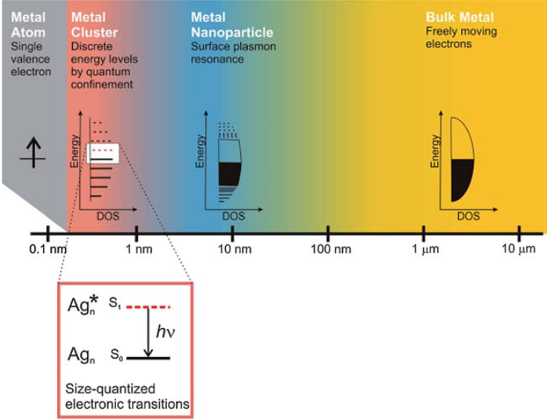
\includegraphics[width=0.7\textwidth]{pictures/metal_NCs.png}
		\caption{Энергетические уровни в металлах разного размера \cite{Dez2011}}
		\label{fig_ncs}
	\end{figure}
	
	Это приводит к дискретной энергетической структуре, что делает их способными к эффективному испусканию света при переходах между уровнями. Энергии переходов при возбуждении кластера описывается энергетическим зазором HOMO-LUMO\footnote{\textbf{H}ighest \textbf{O}ccupied \textbf{M}olecular \textbf{O}rbital и \textbf{L}owest \textbf{U}noccupied \textbf{M}olecular \textbf{O}rbital}, или разницей между низшей незаполненной и высшей заполненной электронной орбиталью:
	
	\begin{flalign} 
		\label{eq1}
		E_g = E_{LUMO} - E_{HOMO}
	\end{flalign}
	
	Сами НК могут различаться как по размеру, насчитывая от одного до нескольких десятков атомов, так и по пространственной структуре. Эти факторы, вместе с зарядом кластера, определяют его фотофизические свойства. В качестве НК часто выступают такие металлы как медь и алюминий \cite{Qing2019}, золото, серебро \cite{Karpushkin2020} и другие.
	
	% Когда молекула/кластер поглощает фотон, электрон переходит из HOMO в LUMO (или выше). Энергия фотона должна быть больше или равна ширине зазора. После релаксации возбужденный электрон возвращается обратно, и разница в энергии между LUMO и HOMO (с учётом потерь на фононы и др.) испускается в виде фотона. Этот эффект и называется люминесценцией. Длина волны испускаемого света зависит от величины $E_g$.
	
	% Металлы в чистом виде стремятся объединиться в крупные объекты. Чтобы добиться частиц металлов, состоящих из нескольких атомов, требуется стабилизация.
	
	В случае биосенсоров, стабилизация кластеров осуществляется при помощи биологических лигандов — белков, полимеров, аминокислот, ДНК и т.д. Введение лигандов зачастую сопровождается изменением квантового выхода люминесценции \cite{Wegeberg2021}. Так, может меняться не только интенсивность, но и длина волны испускаемого излучения.
	
	Нанокластеры можно детектировать различными экспериментальными методами: 
	
	\begin{enumerate}
		\item \textit{Флуоресценция}. Нанокластеры ярко флуоресцируют и часто используются в «turn-on/off» сенсорах. Например, в работе Dong et al. (2025) был создан FRET-датчик на основе Cys-CuNC: кластеры связывали с субстратом ALP и адсорбировали \ce{Cu^{2+}}, меняя флуоресценцию при добавлении PHOS \cite{Dong2025}. Диапазон обнаружения ALP получился 0.1–50 U/L, LOD 0.075 U/L.
		
		\item \textit{SERS\footnote{\textbf{S}urface-\textbf{E}nhanced \textbf{R}aman \textbf{S}pectroscopy — поверхностно-усиленная Рамановская спектроскопия}}. Крупные сборки кластеры–направляющие с металлами (обычно, золотом) обеспечивают усиление Раман-сигнала мишени. Например, прототипы SERS-зондов содержат AgNC на нанощетках, усиливающих спектры
		белковых маркеров инфекций. \cite{Demirel2018}
		
		\item \textit{Масс-спектрометрия}. СТУ-размер кластера позволяет анализ состава (металлы+лиганды) через ESI-MS или MALDI. Это важно для определения размера нанокластера \cite{Gao2023}
		
		\item \textit{Электрохимические сенсоры}. Нанокластеры наносят на электроды для усиления электрического сигнала. Благодаря каталитической активности CuNC и большой	поверхности они повышают токи окисления биомолекул. Так, в недавней работе  описаны биоанализаторы с CuNC, регистрирующие глюкозу, холестерин, белки и др. посредством	модифицированного электрода \cite{Han2025}.
	\end{enumerate}
	
	Главной фотофизической характеристикой, исследуемой в данной работе, является спектр поглощения. Отличительной особенностью небольших металлических кластеров являются узкие вследствие квантованных электронных уровней полосы поглощения  \cite{Wegeberg2021}.
	
	Всё это делает возможным детектирование с помощью НК металлов различных химических соединений — \textbf{биомаркеров}. Биомаркером называется измеряемая характеристика, служащая индикатором нормального или патологического биологического процесса или ответа на воздействие. Это	могут быть молекулы в крови, параметры Функциональной диагностики, генетические и прочие индикаторы \cite{Califf2018}. Биомаркеры используются для диагностики, скрининга, прогнозирования, мониторинга	терапии и превентивных мер. 
	
	\newpage
	
	По назначению биомаркеры разделяют на несколько категорий: 
	\begin{enumerate}
		\item \textit{Диагностический биомаркер} подтверждает наличие или отсутствие заболевания (например, повышенный уровень ПСА указывает на рак простаты \cite{Biomarkers}). 
		\item \textit{Прогностический биомаркер} оценивает вероятность неблагоприятного исхода (например, объем опухоли или индекс Ki-67 при раке прогнозируют агрессивность \cite{Biomarkers2}). 
		\item \textit{Предиктивный биомаркер} предсказывает отклик на лечение (например, мутация EGFR указывает на эффективность ингибиторов EGFR у больных раком легкого  \cite{Biomarkers2}). 
		\item \textit{Мониторинговый биомаркер} измеряют серийно для оценки динамики болезни или действия терапии (например, гликированный HbA1c и артериальное давление при лечении диабета и гипертонии \cite{Califf2018}). 
		\item \textit{Маркеры риска} (susceptibility/risk) идентифицируют лиц с
		повышенным риском заболеть (генетический маркер BRCA1/2, APOE4 и т.п.)  \cite{Califf2018}. 
		\item Также выделяют \textit{фармакодинамические} и \textit{оценки безопасности} (например, пролонгация QT на ЭКГ как маркер риска аритмии при терапии  \cite{Califf2018}).
	\end{enumerate}
	
	Нанокластеры могут использоваться для обнаружения биомаркеров, благодаря сочетания возможности выращивания нанокластеров под конкретные мишени и многократному усилению сигнала при обнаружении этих мишеней. Мишенепривязанность достигается конъюгацией с селективными лигандами (антитела, аптамеры, рецепторные белки), что позволяет кластерам избирательно захватывать аналиты (антиген, ДНК-последовательность) в растворе или на поверхности. Изменение испущенного сигнала обеспечивается оптическими или электрохимическими свойствами: флуоресценция кластера прямо зависит от состояния связи, либо их электрохимическая активность усиливает сигнал. Каждый кластер может генерировать множество фотонов, а также вступать в каталитические циклы, дополнительно повышая чувствительность. Эти механизмы обеспечивают очень низкие пределы обнаружения	(до пико-молей) и высокую селективность.
	
	Преимущества биосенсоров на основе металлических нанокластеров включают:
	\begin{itemize}
		\item \textit{Высокую чувствительность}: благодаря усиленной флуоресценции кластеры позволяют обнаруживать очень низкие концентрации мишеней (pM–nM) \cite{Romeo2021, Han2025}.
		\item \textit{Широкие возможности функционализации}: лиганды и антитела придают специфичность; можно «настраивать» кластеры под любую мишень (бактерию, вирус, белок).
		\item \textit{Стабильность}: в отличие от органических красителей, нанокластеры устойчивы к фото- и химической деградации при правильной стабилизации.
	\end{itemize}
	
	\newpage
	
	При этом, на сегодняшний день, у них есть ряд недостатков:
	\begin{itemize}
		\item \textit{Точность синтеза}: получать строго однородные нанокластеры (по размеру/форме) сложно, что влияет на воспроизводимость сигналов.
		\item \textit{Селективность}: в сложных биосистемах возможна неспецифическая адсорбция белков, что снижает специфичность сенсоров без дополнительных модификаций.
		\item \textit{Токсичность}: AgNCs и CuNCs потенциально токсичны из-за высвобождения ионов металлов, поэтому для
		медицинских применений часто предпочитают AuNCs. Однако, в последнее время продолжилась активная разработка менее токсичных нанокластеров на основе меди \cite{Babu2022}. Более того, цито-токсичность можно обернуть в приемущество путём разработки CuNCs под определённый тип нежелательных клеток, например, раковых \cite{Haiguang2026, Sijia2024}.
		\item \textit{Биодистрибуция}: нанокластеры задерживаются в печени и селезенке, особенно если размер >5–6 нм. Это ограничивает их применение для метаболизма и выведения \cite{Hejazy2018}.
	\end{itemize}
	
	С точки зрения Всемирной Организации Здравоохранения, нанокластеры рассматриваются как медицинские наноматериалы, поэтому они подпадают под общие требования по оценке безопасности лекарств и медицинских устройств. Чтобы получить возможность для широкого применения в медицине, должны быть устранены регуляторные вопросы: отсутствие долгосрочных данных о токсичности, необходимость стандартных протоколов по	оценке наноматериалов. Вследствие новизны технологии, требуется проведения дополнительных испытаний, чтобы доказать клиническую пригодность. 
	
	 Как уже говорилось ранее, нанокластеры обладают свойством специфичности. Их свойства во многом зависят от типа лиганда: тиолятные и пептидные лиганды обеспечивают водорастворимость и биосовместимость, нуклеиновые кислоты – возможность ДНК-темплирования, белки (BSA) – яркую флуоресценцию с различной поляризацией \cite{Han2025, He2025}. 
	
	%	\textbf{\textit{Тут следует расписать, что такое биомаркеры, чем интересы, диагностику каких заболевания позволяют проводить, в том числе с помощью кластеров меди}}
	
	\newpage
	
	\subsection*{Тиоляты}
	\addcontentsline{toc}{subsection}{Тиоляты}
	
	Тиолы и тиоляты — органические соединения с функциональной тиольной/тиолятной группой (т.е. молекулы вида RSH/RS-, где R — органический радикал). К тиолам относятся множество важных веществ в нашем организме:
	
	\begin{enumerate}
		\item \textbf{Глутатион (GSH)} — главный внутриклеточный антиоксидант, наиболее важное тиоловое соединение внутри клеток. Глутатион состоит из трех аминокислот и обладает уникальной способностью «жертвовать» электрон свободным радикалам, нейтрализуя их. GSH защищает ДНК и митохондрии от повреждений, восстанавливает другие антиоксиданты (витамины C и E) и участвует в работе печени по очистке крови. Низкий уровень глутатиона напрямую связан с быстрым старением и хроническими заболеваниями.
		\cite{TOWNSEND2003145}.
		\item \textbf{Цистеин} — серосодержащая аминокислота, необходимая для синтеза белков и глутатиона. Формирует дисульфидные мостики в белках. Так например, прочность волос, ногтей и кожи на 10–14\% зависит от цистеина в составе кератина. \cite{Sohrab2021, Cysteine}. У цистеина есть множество различных применений. Так, его производное — N-ацетилцистеин (АЦЦ) — часто используют как лекарство, разжижающее мокроту легких.
		\item \textbf{Кофермент А} — ключевое звено в процессах окисления жирных кислот и получения энергии из пищи. Он переносит углеродные фрагменты в митохондрии. Без него невозможен цикл Кребса — главный процесс производства АТФ \cite{ijms21239057}. 
		\item \textbf{Гомоцистеин} — промежуточный продукт метаболизма; его избыток в крови связан с риском сердечно-сосудистых заболеваний. Это промежуточный продукт, который образуется при переработке аминокислоты метионина. В норме он быстро превращается в полезные вещества. Если гомоцистеина становится слишком много (гипергомоцистеинемия), он начинает повреждать стенки сосудов, вызывая воспаление и тромбы. Для снижения его уровня в сосудах критически важны витамины B12 и фолиевая кислота \cite{Kumar2017}.
	\end{enumerate}
	
	По концентрации тиолов в биологических жидкостях (крови, плазме) можно судить о наличии различных заболеваний, включая сердечно-сосудистые патологии и воспалительные процессы. Снижение уровня общего тиолового статуса часто указывает на истощение защитных ресурсов организма.
	
	Тиолятные лиганды играют ключевую роль в стабилизации медных НК и формировании их электронных и оптических свойств. Благодаря высокой аффинности серы к меди, связь Cu–S является прочной и направленной, что обеспечивает эффективную пассивацию поверхности кластера и предотвращает агрегацию. В отличие от более крупных НЧ, где лиганды в основном выполняют стабилизирующую функцию, в ультрамалых кластерах состава $Cu_2$, $Cu_4$, $Cu_8$ тиоляты также непосредственно участвуют в формировании электронной структуры и вносят вклад в природу низкоэнергетических электронных переходов.
	
	\newpage
	
	\subsection*{Квантово-химические вычисления}
	\addcontentsline{toc}{subsection}{Квантово-химические вычисления}
	
	Основной идеей данной работы является сравнительный анализ работы различных DFT-функционалов (с D3 поправкой на дисперсионные взаимодействия \cite{Grimme2010}). В качестве метода для оптимизации структур выбран \textit{ab initio} метод теории возмущений второй степени MP2 с поправкой RI (resolution of identity). Для всех расчётов был использовался базис def2-TZVP \cite{Hellweg2015}. 
	
	Исходя из данных масс-спектрометрии \cite{Jia2013} (см. Рис. \ref{fig_cu_mass_spec}), доминирующими структурами в растворе являются слабо-люминесцирующий комплекс с ионом меди (\ce{[CuL2]^{-1}}, где L=\ce{SCH3}), а также еще один — с двумя атомами меди, стабилизированными двумя лигандами \ce{[Cu2L2]^{-2}}). Для полноты описания, кроме данной структуры, были рассмотрены ещё несколько, а именно: \ce{[Cu3L2]^{-1}}, \ce{[Cu4L3]^{-1}} и \ce{[Cu5L4]^{-1}}. В качестве исходных геометрий были взяты ранее исследованные кластеры серебра на тиолятах из работы \cite{Buglak2019}. 
	
	\begin{figure}[H]
		\centering
		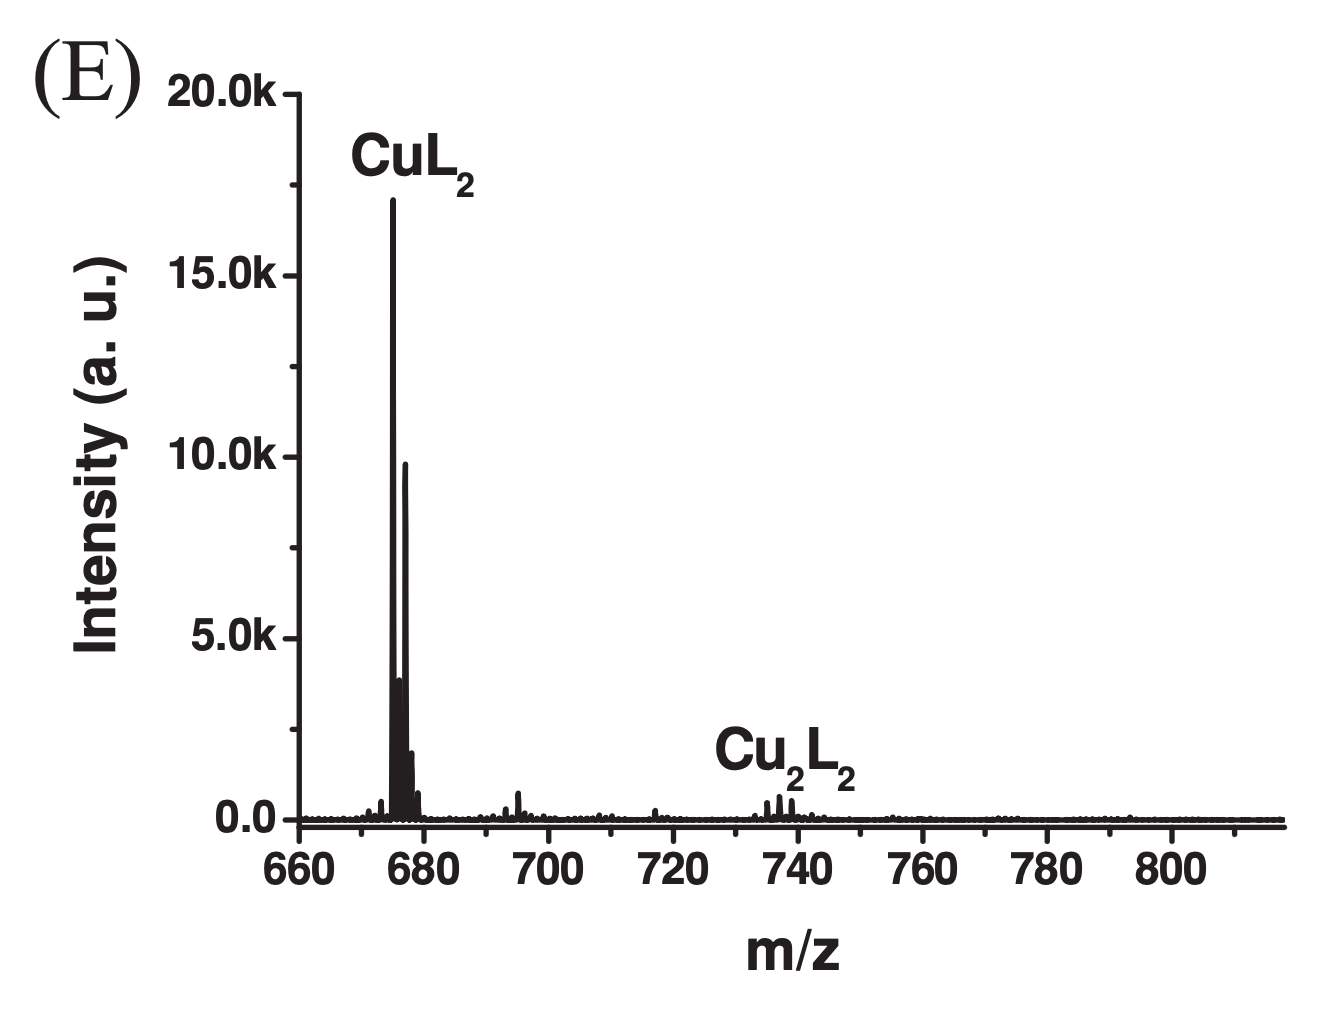
\includegraphics[width=0.5\textwidth]{figures/cu_mass_spec.png}
		\caption{Масс-спектрометрия раствора с НК меди, кэпированных цистеином \cite{Jia2013}.}
		\label{fig_cu_mass_spec}
	\end{figure}
	
	Теоретическое описание методов теории возмущений сводится к поправке энергии и волновых функций молекулы, рассчитанных при помощи метода Хартри-Фока. В качестве малого возмущения изменение потенциала электрон-ядерного взаимодействия при отказе от приближения Борна-Оппенгеймера. Первая поправка уже учтена в методе Хартри-Фока, а вторая, после всех преобразований, запишется в виде:
	
	\begin{equation}
		\label{eq_mp2}
		{ E_0^{(2)} = \frac14 \sum_{a,b} \sum_{n_1, n_2} \frac{|\langle ab||n_1n_2\rangle|^2}{E_a^{(0)} + E_b^{(0)} - E_{n_1}^{(0)} - E_{n_2}^{(0)}} = \frac14\sum_{a,b} \langle ab||n_1n_2\rangle t_{n_1, n_2}^{a, b} },
	\end{equation}
	
	где $a,b$ — виртуальные орбитали, а $n_1, n_2$ — занятые. В данном выражении используется следующая запись ($\psi (a)  = \varphi_\alpha (r_a)\cdot \alpha$ — спин-орбиталь):
	
	\begin{multline}
		\langle ab||n_1n_2\rangle = \langle ab|n_1n_2\rangle - \langle ab|n_2n_1\rangle = \\
		= \iint \psi^*_a(1)\psi_b^*(2)\frac1{r_{12}} \psi_{n_1}(1)\psi_{n_2}(2) d\tau_1 d\tau_2 + \iint \psi^*_a(1)\psi_b^*(2)\frac1{r_{12}} \psi_{n_2}(1)\psi_{n_1}(2) d\tau_1 d\tau_2.
	\end{multline}
	
	А коэффициент $t_{n_1n_2}^{a,b}$ называется тензорной амплитудой и отражает вероятность перехода $n_1\rarr a$ и $n_2 \rarr b$:
	
	\begin{equation}
		\label{eq_tensor_amp}
		t_{n_1, n_2}^{a,b} = \frac{\langle n_1n_2||ab\rangle}{E_a^{(0)} + E_b^{(0)} - E_{n_1}^{(0)} - E_{n_2}^{(0)}}
	\end{equation}
	
	Метод связанных кластеров (CC) появился в результате попытки описать взаимодействие протонов и нейтронов в ядерной физике. Является более точным, но также и более сложным, чем теория возмущений Мёллера-Плессета ($O(N^6)$ в сравнении с $O(N^5)$, где $N$ — число базисных функций). Основная идея метода заключается в поиске волновой функции в следующем виде:
	
	\begin{equation}
		\psi_{CC} = e^{\hat T} \Phi_0
	\end{equation}
	
	Здесь $\hat T$ — \textit{оператор кластера}: $\hat T = \hat T_1 + \hat T_2 + \hat T_3 + \dots $ (где $\hat T_i$ — i-частичное возбуждение). Подставляя волновые функции в таком виде в уравнение Шрёдингера можем получить уравнение на $\Phi_0$:
	
	\begin{equation}
		\hat H \psi_{CC} = E\psi_{CC} \Lrarr \hat H e^{\hat T}\Phi_0 = E e^{\hat T}\Phi_0 \xrightarrow[]{|\cdot e^{-\hat T}} \underbrace{e^{-\hat T} \hat H e^{\hat T}}_{\overline H} \Phi_0 = E \Phi_0
	\end{equation}
	
	$\overline H$ — simmilarity-transformed Hamiltonian, его можно представить в виде разложения Бейкера-Кэмпбелла-Хаусдорфа (BCH):
	
	\begin{equation}
		\label{eq_BCH}
		\overline H = e^{-\hat T} \hat H e^{\hat T} = \hat H + [\hat H, \hat T] + \frac1{2!}\big[[\hat H, \hat T], \hat T\big] + \frac1{3!}\Big[\big[[\hat H, \hat T], \hat T\big], \hat T\Big] + \dots
	\end{equation}
	
	Энергетические уровни в методе связанных кластеров можно записать в виде:
	
	\begin{equation}
		E_{CC} = \langle\Phi_0|e^{-\hat T}\hat H e^{\hat T}|\Phi_0\rangle = \langle\Phi_0|\overline H|\Phi_0\rangle 
	\end{equation}
	
	В приближении, где мы учитываем возбуждения, не более двухчастичных (CCSD\footnote{\textbf{C}oupled \textbf{C}lusters \textbf{S}ingles and \textbf{D}oubles}). получим следующее выражение для полной энергии:
	
	\begin{equation}
		E_{CCSD}= \langle\Phi_0|e^{-\hat T}\hat H e^{\hat T}|\Phi_0\rangle = E_{HF} + \sum_{i}\sum_{a}t_{i}^{a}f_{ia} + \frac14 \sum_{i,j}\sum_{a,b}\tau_{ij}^{ab}\langle ij||ab\rangle
	\end{equation}
	
	В настоящее время «золотым стандартом» для квантово-химических вычислений является метод CCSD(T), являющийся методом CCSD с рассчитанными по методу теории возмущений трёхчастичными взаимодействиями. Хотя он и обеспечивает расчет $\sim99\%$ корреляционной энергии, но является критически требователен к ресурсам (имеет сложность $O(N^7)$). Поэтому в данной работе в качестве референса был выбран метод EOM-CCSD.
	
	В данном полученном выражении для энергии $\tau_{ij}^{ab} = t_{ij}^{ab} + t_i^at_j^b - t_i^bt_j^a$, а $f_{ia}$ — матричные элементы матрицы фока $\hat F$ ($\hat F_i \varphi_i = E_i \varphi_i$). Стоит отметить, что метод связанных кластеров будет сходиться при большой разнице между возбуждёнными и виртуальными орбиталями. Например, для расчёта сплошных металлов он не подходит.
	
	Поправка RI вводится для ускорения вычислений. Рассмотрим обменный интеграл вида:
	
	$$
	\langle \Phi_{ij}(\vec r_1) | \frac1{r_{12}}| \Phi_{kl}(\vec r_2) \rangle,
	$$
	
	где: 
	
	$$
	\Phi_{\lambda \sigma}(\vec r_1) = \varphi_i \varphi_j = \sum_i \sum_j C_\lambda ^{(i)} C_\sigma ^{(j)} \varphi^{b,\ i}_\lambda \varphi^{b,\ j}_\sigma 
	$$
	
	Раскрывая данное выражение получим четыре суммы, что требует больших вычислительных затрат. Идея RI заключается в аппроксимации $\Phi_{ij}$ через некоторый новый базис  $\Phi_a^{tr}$\footnote{здесь $^{tr}$ указывает на trial, пробную функцию}(который часто обозначается как auxilary basis):
	
	$$
	\Phi_{ij}(\vec r_1) = \sum_{a}\widetilde{C}_a \Phi_a^{tr}
	$$
	
	Даже при повторном разложении по дополнительному базису, погрешность всё равно будет меньше, чем в методе DFT. Это позволяет достичь большей точности при сравнительно малом различии во времени вычисления, что существенно для расчётов характеристик соединений высокоуровневыми методами (например, методом связанных кластеров и его производных: EOM-CCSD, CC2, ADC2  и др.).
	
	Теория функционала плотности, или DFT, разработанная Уолтерем Коном и Пьером Хонбергом еще в XX веке \cite{HoenbergKohn1964}, является одним из наиболее распространённых теоретических методов исследования. В нём ключевую роль играет электронная плотность, которую вводят взамен обменного интеграла, зависящего от волновых функций отдельных электронов. Хонберг и Кон доказали теорему, согласно которой энергия основного состояния молекул является функционалом электронной плотности и энергия минимальна, если эта плотность является точной электронной плотностью основного состояния. То есть, существует функция $\rho$ такая, что:
	
	\begin{equation}
		E[\rho] = F[\rho] + \int V_{ext}(\vec r)\rho (\vec r) d\vec r,
	\end{equation}
	
	где $V_{ext}$ — внешний потенциал, а $F$ — некоторый универсальный функционал. Практическая реализация Кона и Шема \cite{KohnSham1965}, т.н. KS DFT, заключается в разложении обменного интеграла электрон-ядерной системы на две составляющие. Таким образом, в данном представлении электронная плотность основного состояния представлена в виде:
	
	\begin{equation}
		E[\rho] = T_s[\rho] + E_{nl}[\rho] + J[\rho] + E_{xc}[\rho],
	\end{equation}
	
	которая теперь состоит из следующих составляющих:
	
	\begin{enumerate}
		\item[—] $E_{nl}[\rho] = \int V_{ext}(\vec r) \rho(\vec r)\ d\vec r$ — электрон-ядерное взаимодействие;
		\item[—] $J[\rho] = \frac12 \iint \frac{\rho(\vec r_1)\rho(\vec r_2)}{|\vec r_1 - \vec r_2|} d\vec r_1 d\vec r_2$ — обменный член из метода Хартри-Фока;
		\item[—] $T_s[\rho] = \sum_{i=1}^N \int \varphi_i^* (\vec r) (-\frac12\vec \nabla^2)\varphi_i(\vec r)\ d\vec r$ — оператор кинетической энергии не взаимодействующих электронов
		\item[—] $E_{xc}[\rho]$ — обменно-корреляционный функционал, учитывающий также отличие кинетической энергии $T$ от $T_s$. Подбирается полу-эмпирически и на самом деле $E_{xc}[\rho,\vec \nabla \rho]$. Одним из вариантов является расчёт модельных систем более точным методом и подгонка функционала по полученным результатам. Также, для данных целей могут использоваться методы машинного обучения и, в частности, нейронные сети.
	\end{enumerate}
	
	Дальнейшее развитие этой теории заключается в применении метода градиентной коррекции, который учитывает производные электронной плотности при расчёте кинетической и потенциальной энергии молекул. Как следствие, данные методы квантовой химии активно развиваются и используются сегодня.
	
	Стоит отметить, что существуют различные вариации теории функционала плотности. Наиболее быстрым является класс orbital-free DFT. В нём происходит отказ от обменного вклада, рассчитанного при помощи волновых функций электронов. В результате, остается только полу-эмпирический вклад в $E_{xc}[\rho]$. Однако на практике, в чистом виде он не используется.
	
	Наибольшее распространение получили гибридные методы, оставляющие как полуэмпирический, так и Хартри-Фоковский (ХФ) корреляционные вклады. Варьируя влияние этих двух вкладов, можно добиться желаемого баланса точности и скорости расчётов. Для сравнения были выбраны следующие функционалы: 
	\begin{enumerate}
		\item $M06-2X$ с 54\% вкладом ХФ;
		\item $CAM-B3LYP$ с 19\% ХФ вкладом на коротких расстояниях и 65\% на длинных  \cite{Yanai2004};
		\item $PBE0$, являющийся модифицированной версией $PBE$ \cite{Perdew1996} с 25\% ХФ вкладом \cite{Ernzerhof1999};
		\item $\omega B97X$  \cite{Chai2008};
		\item $BHandHLYP$, являющийся комбинацией обменного функционала Becke, 50-процентного ХФ вклада и корреляционного функционала Lee-Yang-Par \cite{Parr1989}.
		%		\item $r^2SCAN50$  с 50\% вкладом ХФ \cite{Bursch2022}. 
	\end{enumerate}
	
	При помощи этих методов становится возможным определение многих свойств молекул, таких как длины межатомных расстояний, энергии связи, спектров поглощения, спектров комбинационного рассеяния и т.д.
	
	% В этой работе использовались функционалы Бекке—Ли—Янга—Парра (B3LYP)
	
	% \cite{Perdew1996}
	
	\newpage
	
	\section*{Методы исследования}
	\addcontentsline{toc}{section}{МЕТОДЫ ИССЛЕДОВАНИЯ}
	
	В ходе работы проведено теоретическое исследование комплексов меди с тиолятами. На различных этапах использованы следующие программы:
	\begin{enumerate}
		\item Построение структур комплексов и визуализация результатов, в частности модельных спектров и оптимизированных структур, выполнена в программе Chemcraft\ths1.8.
		\item Оптимизация геометрии и моделирование спектров поглощения выполнены в программном пакете ORCA 6.0 \cite{ORCA6}.
		\item Обработка спектров осуществлена в программе OriginPro\ths2024
	\end{enumerate}
	
	Моделирование спектров выполнено как в газовой фазе, так и в воде. В качестве модели растворителя использована континуальная модель воды CPCM \cite{ORCA_cpcm_1}. Основными параметрами модели являются диэлектрическая проницаемость и показатель преломления — $\varepsilon$ и $n$ соответственно. Для воды $\varepsilon=80,4$ и $n=1,33$ \cite{ORCA_cpcm_2}.
	
	Бенчмаркинг пяти вышеперечисленных DFT функционалов осуществлялся в газовой фазе относительно эталонного \textit{ab-initio} метода DLPNO-STEOM-CCSD. После получения модельных спектров поглощения, были рассчитаны среднеквадратичные отклонения (RMSE\footnote{Residual Mean Squared Error}) для всех расчётных переходов и отдельно для самого длинноволнового HOMO $\rarr$ LUMO перехода.
	
	\newpage
	
	\section*{Результаты и обсуждение}
	\addcontentsline{toc}{section}{РЕЗУЛЬТАТЫ И ОБСУЖДЕНИЕ}
	
	В работе исследованы 5 комплексов:  \ce{[CuL2]^{-1}}, \ce{[Cu2L2]^{-2}}, \ce{[Cu3L2]^{-1}}, \ce{[Cu4L3]^{-1}} и \ce{[Cu5L4]^{-1}}. В качестве лигандов \ce L применялись различные структуры. В простейшем приближении рассмотрена метилтиогруппа \ce{SCH_3}. Помимо этого, были оптимизированы структуры с цистеином (\ce{Cys}) в роли тиола. Для всех комплексов получены оптимизированные геометрии и UV-VIS спектры поглощения. Моделирование проведено для газовой фазы и имплицитного растворителя (воды). 
	
	\subsection*{Комплексы с метилтиогруппой}
	\addcontentsline{toc}{subsection}{Комплексы с метилтиогруппой}
	
	\subsubsection*{Оптимизированные геометрии}
	% \addcontentsline{toc}{subsubsection}{Оптимизированные геометрии}
	
	Оптимизированные структуры представлены на Рис.\ths\ref{fig_geoopt_SCH3_vac}. В Таблицах \ref{tab1}, \ref{tab2} и \ref{tab3} приведены основные структурные параметры комплексов, вместе с разностью значений, полученных в вакууме и воде. Рассмотрим каждый комплекс по-отдельности.
	
	\begin{figure}[H]
		\centering
		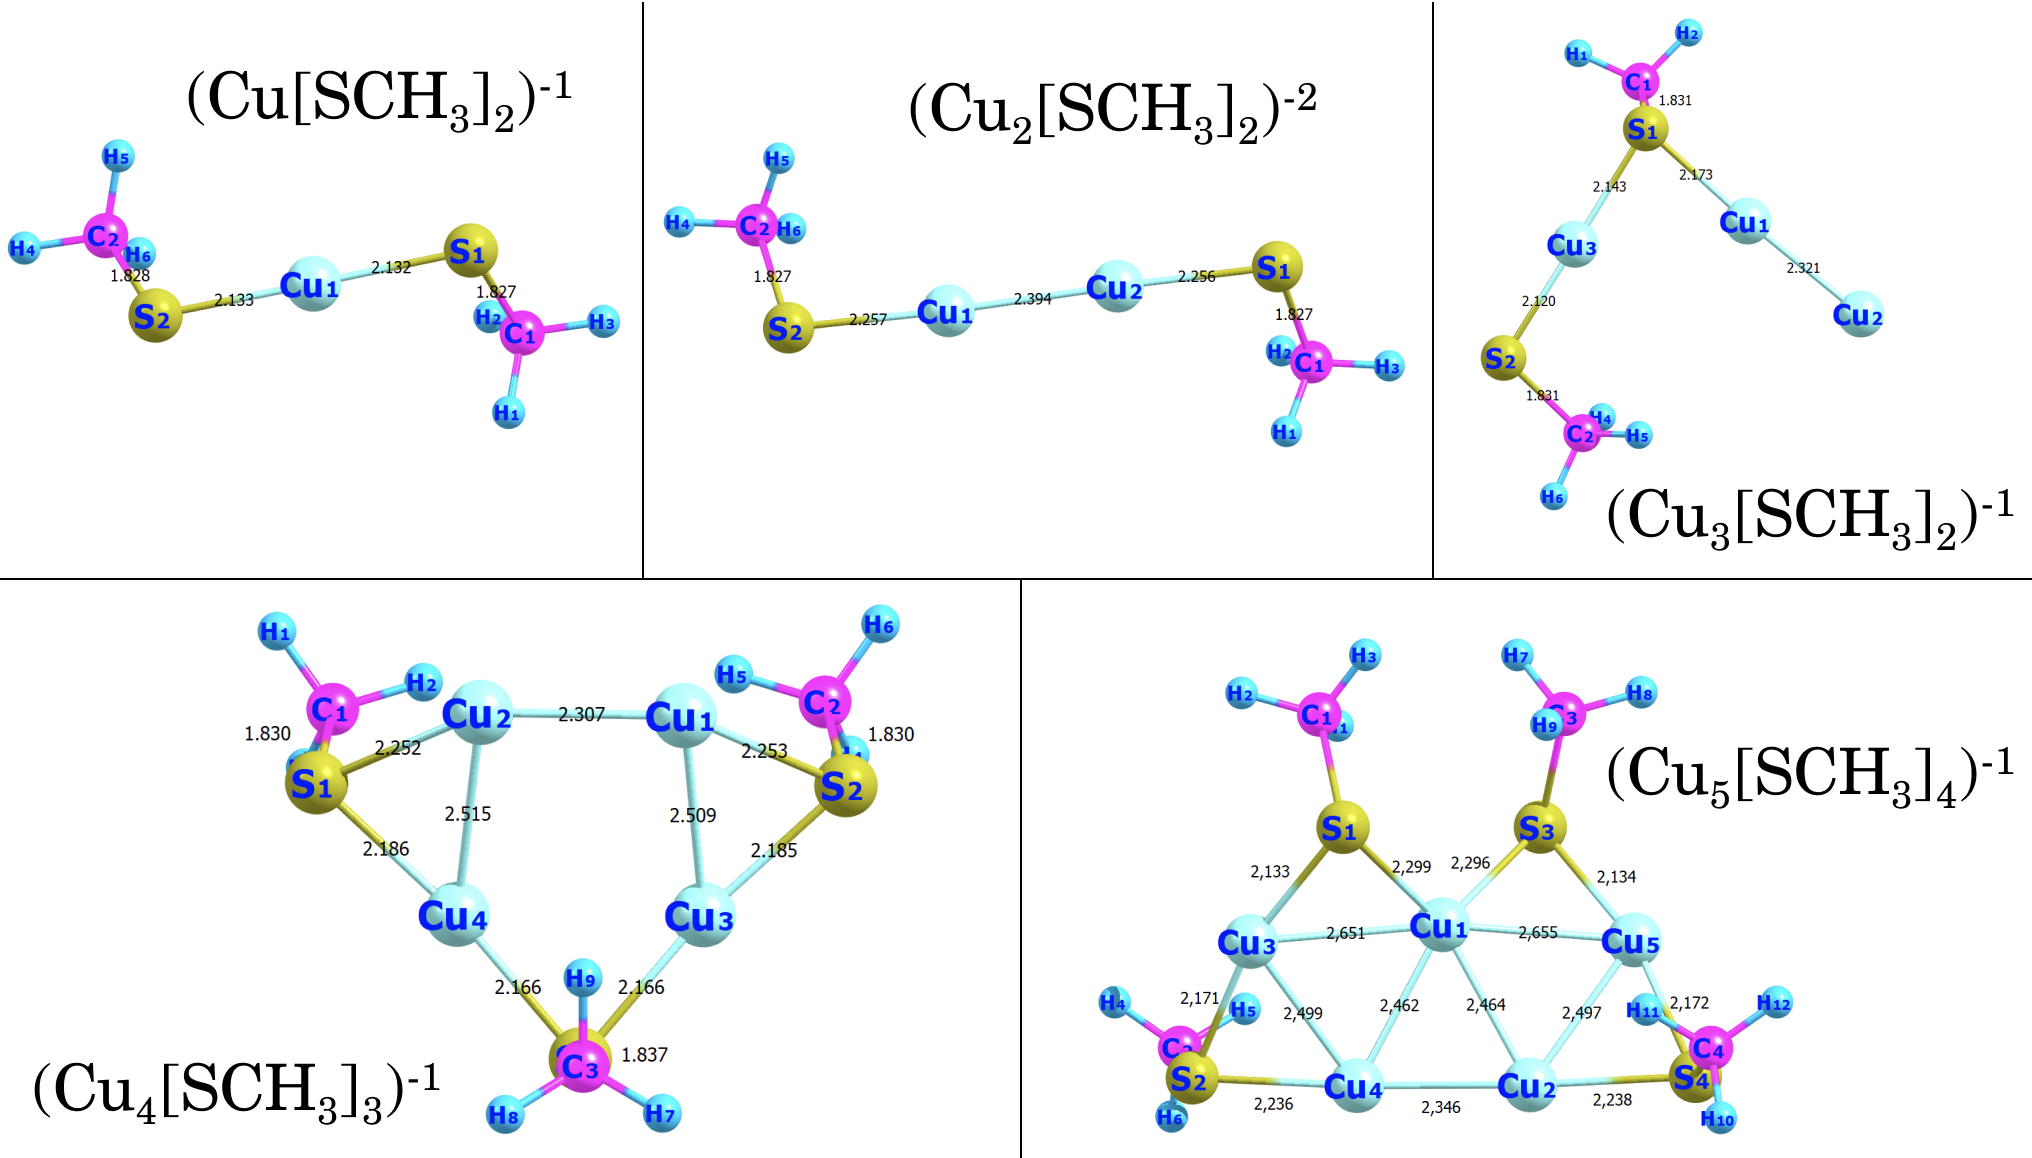
\includegraphics[width=\textwidth, frame]{pictures/opt_SCH3_vac.jpg}
		\caption{Оптимизированные {в вакууме} геометрии комплексов, стабилизированных метилтиогруппой (метод: MP2 def2-TZVP).}
		\label{fig_geoopt_SCH3_vac}
	\end{figure}
	
	Для комплекса \ce{[Cu(SCH3)2]^{-1}} длины связей, полученные в газовой фазе и воде, не сильно отличаются: максимальное различие составляет 0,006Å для связи C1-S1. Валентные углы также отличаются несущественно, разность между расчётами в воде и вакууме варьируется в диапазоне 0,01-0,08º. Для двугранных углов разность составляет не более 14,6º. Стоит отметить, что визуально структуры крайне похожи. 
	
	Рассмотрим комплекс \ce{[Cu2(SCH3)2]^{-2}}. Даже не вооруженным взглядом видны отличия в оптимизации в воде и газовой фазе: вместо относительно линейной структуры в вакууме, геометрия молекулы в воде искажена. Это же отражено и в таблице, различия углов стали на два порядка больше, по сравнению с комплексом с одним атомом меди (максимальная разность составляет 4,8º). Ситуация со связями также изменилась. Длины связей C1-S1 и C2-S2 в воде стали ещё выше, чем для предыдущей структуры. При этом, результаты в вакууме практически не изменились. Забегая вперёд, длины связей C-S для всех комплексов практически всегда больше в воде, однако различие в разности наблюдается только в третьем знаке, что можно списать на погрешность расчётов. В воде связи Cu-S получились значительно короче, в сравнении с вакуумом (на 0,070Å для S2-Cu1 и 0,073Å для S1-C2). Эта же динамика наблюдается и для связи Cu-Cu, которая сократилась на 0,039Å в воде. Двугранные углы различаются не более, чем на 10,8º.
	
	\begin{table}[H]
		\caption{Основные структурные параметры комплексов \ce{[Cu(SCH3)2]^{-1}} и \ce{[Cu2(SCH3)2]^{-2}}.}
		\label{tab1}
		\centering
		\begin{tabular}{ccccc|cccc|}
			\cline{1-4} \cline{6-9}
			\multicolumn{4}{|c|}{\textbf{\ce{[Cu(SCH3)2]^{-1}}}}                                                                                            & \textbf{} & \multicolumn{4}{c|}{\textbf{\ce{[Cu2(SCH3)2]^{-2}}}}                                                                       \\
			\cline{1-4} \cline{6-9}
			\multicolumn{4}{|c|}{\textit{длины связей (Å)}}                                                                               & \textit{} & \multicolumn{4}{c|}{\textit{длины связей (Å)}}                                                           \\ \cline{1-4} \cline{6-9} 
			\multicolumn{1}{|c|}{атомы}        & \multicolumn{1}{c|}{вакуум} & \multicolumn{1}{c|}{вода}  & \multicolumn{1}{c|}{разность} &           & \multicolumn{1}{c|}{атомы}         & \multicolumn{1}{c|}{вакуум} & \multicolumn{1}{c|}{вода}  & разность \\ \cline{1-4} \cline{6-9} 
			\multicolumn{1}{|c|}{C2-S2}        & \multicolumn{1}{c|}{1,828}  & \multicolumn{1}{c|}{1,833} & \multicolumn{1}{c|}{-0,005}   &           & \multicolumn{1}{c|}{C2-S2}         & \multicolumn{1}{c|}{1,827}  & \multicolumn{1}{c|}{1,836} & -0,009   \\ \cline{1-4} \cline{6-9} 
			\multicolumn{1}{|c|}{C1-S1}        & \multicolumn{1}{c|}{1,827}  & \multicolumn{1}{c|}{1,833} & \multicolumn{1}{c|}{-0,006}   &           & \multicolumn{1}{c|}{C1-S1}         & \multicolumn{1}{c|}{1,827}  & \multicolumn{1}{c|}{1,835} & -0,008   \\ \cline{1-4} \cline{6-9} 
			\multicolumn{1}{|c|}{S2-Cu1}       & \multicolumn{1}{c|}{2,133}  & \multicolumn{1}{c|}{2,129} & \multicolumn{1}{c|}{0,004}    &           & \multicolumn{1}{c|}{S2-Cu1}        & \multicolumn{1}{c|}{2,257}  & \multicolumn{1}{c|}{2,187} & 0,070    \\ \cline{1-4} \cline{6-9} 
			\multicolumn{1}{|c|}{S1-Cu1}       & \multicolumn{1}{c|}{2,132}  & \multicolumn{1}{c|}{2,13}  & \multicolumn{1}{c|}{0,002}    &           & \multicolumn{1}{c|}{S1-Cu2}        & \multicolumn{1}{c|}{2,256}  & \multicolumn{1}{c|}{2,183} & 0,073    \\ \cline{1-4} \cline{6-9} 
			\multicolumn{4}{|c|}{\textit{валентные углы (º)}}                                                                             & \textit{} & \multicolumn{1}{c|}{Cu1-Cu2}       & \multicolumn{1}{c|}{2,394}  & \multicolumn{1}{c|}{2,355} & 0,039    \\ \cline{1-4} \cline{6-9} 
			\multicolumn{1}{|c|}{атомы}        & \multicolumn{1}{c|}{вакуум} & \multicolumn{1}{c|}{вода}  & \multicolumn{1}{c|}{разность} &           & \multicolumn{4}{c|}{\textit{валентные углы (º)}}                                                         \\ \cline{1-4} \cline{6-9} 
			\multicolumn{1}{|c|}{C2-S2-Cu1}    & \multicolumn{1}{c|}{103,8}  & \multicolumn{1}{c|}{103,8} & \multicolumn{1}{c|}{0,1}      &           & \multicolumn{1}{c|}{атомы}         & \multicolumn{1}{c|}{вакуум} & \multicolumn{1}{c|}{вода}  & разность \\ \cline{1-4} \cline{6-9} 
			\multicolumn{1}{|c|}{S2-Cu1-S1}    & \multicolumn{1}{c|}{179,4}  & \multicolumn{1}{c|}{179,4} & \multicolumn{1}{c|}{0,0}      &           & \multicolumn{1}{c|}{C2-S2-Cu1}     & \multicolumn{1}{c|}{100,1}  & \multicolumn{1}{c|}{97,1}  & 3,0      \\ \cline{1-4} \cline{6-9} 
			\multicolumn{1}{|c|}{C1-S1-Cu1}    & \multicolumn{1}{c|}{104,1}  & \multicolumn{1}{c|}{104,1} & \multicolumn{1}{c|}{0,0}      &           & \multicolumn{1}{c|}{S2-Cu1-Cu2}    & \multicolumn{1}{c|}{177,6}  & \multicolumn{1}{c|}{172,8} & 4,8      \\ \cline{1-4} \cline{6-9} 
			\multicolumn{4}{|c|}{\textit{дигедральные углы   (º)}}                                                                        & \textit{} & \multicolumn{1}{c|}{S1-Cu2-Cu1}    & \multicolumn{1}{c|}{178,3}  & \multicolumn{1}{c|}{175,6} & 2,6      \\ \cline{1-4} \cline{6-9} 
			\multicolumn{1}{|c|}{атомы}        & \multicolumn{1}{c|}{вакуум} & \multicolumn{1}{c|}{вода}  & \multicolumn{1}{c|}{разность} &           & \multicolumn{1}{c|}{C1-S1-Cu2}     & \multicolumn{1}{c|}{100,5}  & \multicolumn{1}{c|}{98,9}  & 1,6      \\ \cline{1-4} \cline{6-9} 
			\multicolumn{1}{|c|}{C2-S2-Cu1-S1} & \multicolumn{1}{c|}{-80,0}  & \multicolumn{1}{c|}{-70,9} & \multicolumn{1}{c|}{-9,2}     &           & \multicolumn{4}{c|}{\textit{дигедральные углы (º)}}                                                      \\ \cline{1-4} \cline{6-9} 
			\multicolumn{1}{|c|}{C1-S1-Cu1-S2} & \multicolumn{1}{c|}{164,5}  & \multicolumn{1}{c|}{149,8} & \multicolumn{1}{c|}{14,6}     &           & \multicolumn{1}{c|}{атомы}         & \multicolumn{1}{c|}{вакуум} & \multicolumn{1}{c|}{вода}  & разность \\ \cline{1-4} \cline{6-9} 
			&                             &                            &                               &           & \multicolumn{1}{c|}{C2-S2-Cu1-Cu2} & \multicolumn{1}{c|}{-11,3}  & \multicolumn{1}{c|}{-4,7}  & -6,6     \\ \cline{6-9} 
			&                             &                            &                               &           & \multicolumn{1}{c|}{C1-S1-Cu2-Cu1} & \multicolumn{1}{c|}{-0,4}   & \multicolumn{1}{c|}{-8,2}  & 7,8      \\ \cline{6-9} 
			&                             &                            &                               &           & \multicolumn{1}{c|}{S2-Cu1-Cu2-S1} & \multicolumn{1}{c|}{117,6}  & \multicolumn{1}{c|}{128,5} & -10,8    \\ \cline{6-9} 
		\end{tabular}
	\end{table}
	
	В структуре \ce{[Cu3(SCH3)2]^{-1}} наблюдается противоположное изменение: все связи Cu-S увеличились в воде (для Cu3-S2, Cu3-S1 и Cu1-S1 на 0,012Å, 0,017Å и 0,011Å соответственно). Валентные углы изменились не значительно, в среднем изменение составило 2,3º, а максимальная разность — 5,8º. Стоит отметить, что значительнее всего изменились углы между связями, содержащими медь: Cu1-S1-Cu3 и S1-Cu1-Cu2. Для двугранных углов наблюдаются значительные изменения: углы Cu3-S1-Cu1-Cu2 и C1-S1-Cu1-Cu2 изменились на 32,6º и 35,6º соответственно. Это изменение можно наблюдать наглядно, структура в воде искажена и сжата в сравнении с вакуумом. Остальные двугранные углы значительно не изменились, разности согласуются с значениями для предыдущих комплексов.
	
	Для структур \ce{[Cu4(SCH3)3]^{-1}} и \ce{[Cu5(SCH3)4]^{-1}} рассмотрены только длины связей. Для комплекса с четырёхатомным кластером меди наиболее явно различаются связи Cu-S: S1-Cu4 и S2-Cu3, S2-Cu1 и S1-Cu2 (Рис. \ref{fig_geoopt_SCH3_vac}). Для первой пары длина связи в воде увеличилась и разность составила порядка -0,025Å, а для второй — 0,042Å, что свидетельствует об уменьшении длины связи. Однако, расстояния Cu3-S3 и Cu4-S3 практически не изменились, разность составила -0,007Å. Длины связей Cu-Cu увеличились в воде, однако незначительно: максимальное изменение составило -0,009Å для связи Cu1-Cu2.
	
	Для комплекса с пятиатомным кластером меди наблюдается схожая картина: связи S1-Cu1 и S3-Cu1 сильно сократились в воде (на 0,040Å и 0,038Å соответственно). Длины связей S2-Cu4 и S4-Cu2 уменьшились на 0,009Å и 0,011Å соответственно, а S2-Cu3, S3-Cu5 и S4-Cu5 увеличились на 0,008Å, 0,010Å и 0,008Å соответственно. Рассматривая связи Cu-Cu, наблюдается весьма интересная картина: связи Cu1-Cu3 и Cu1-Cu5 значительно сократились в воде, Cu1-Cu4, Cu1-Cu2 и Cu4-Cu2 — существенно увеличились, а длины связей Cu3-Cu4 и Cu2-Cu5 практически не изменились.
	
	\begin{table}[H]
		\caption{Основные структурные параметры комплексов \ce{[Cu3(SCH3)2]^{-1}} и \ce{[Cu5(SCH3)4]^{-1}}.}
		\label{tab2}
		\centering
		\begin{tabular}{|cccc|ccccc}
			\cline{1-4} \cline{6-9}
			\multicolumn{4}{|c|}{\textbf{\ce{[Cu3(SCH3)2]^{-1}}}}                                                                         & \multicolumn{1}{c|}{} & \multicolumn{4}{c|}{\textbf{\ce{[Cu5(SCH3)4]^{-1}}}}                                                                                     \\ \cline{1-4} \cline{6-9} 
			\multicolumn{4}{|c|}{\textit{длины связей (Å)}}                                                            & \multicolumn{1}{c|}{} & \multicolumn{4}{c|}{\textit{длины связей (Å)}}                                                                               \\ \cline{1-4} \cline{6-9} 
			\multicolumn{1}{|c|}{атомы}          & \multicolumn{1}{c|}{вакуум} & \multicolumn{1}{c|}{вода}  & разность & \multicolumn{1}{c|}{} & \multicolumn{1}{c|}{атомы}   & \multicolumn{1}{c|}{вакуум}   & \multicolumn{1}{c|}{вода}     & \multicolumn{1}{c|}{разность} \\ \cline{1-4} \cline{6-9} 
			\multicolumn{1}{|c|}{C2-S2}          & \multicolumn{1}{c|}{1,831}  & \multicolumn{1}{c|}{1,835} & -0,004   & \multicolumn{1}{c|}{} & \multicolumn{1}{c|}{C1-S1}   & \multicolumn{1}{c|}{1,828}    & \multicolumn{1}{c|}{1,831}    & \multicolumn{1}{c|}{-0,003}   \\ \cline{1-4} \cline{6-9} 
			\multicolumn{1}{|c|}{C1-S1}          & \multicolumn{1}{c|}{1,831}  & \multicolumn{1}{c|}{1,834} & -0,003   & \multicolumn{1}{c|}{} & \multicolumn{1}{c|}{C2-S2}   & \multicolumn{1}{c|}{1,833}    & \multicolumn{1}{c|}{1,836}    & \multicolumn{1}{c|}{-0,003}   \\ \cline{1-4} \cline{6-9} 
			\multicolumn{1}{|c|}{S2-Cu3}         & \multicolumn{1}{c|}{2,120}  & \multicolumn{1}{c|}{2,132} & -0,012   & \multicolumn{1}{c|}{} & \multicolumn{1}{c|}{C3-S3}   & \multicolumn{1}{c|}{1,828}    & \multicolumn{1}{c|}{1,830}    & \multicolumn{1}{c|}{-0,002}   \\ \cline{1-4} \cline{6-9} 
			\multicolumn{1}{|c|}{S1-Cu3}         & \multicolumn{1}{c|}{2,143}  & \multicolumn{1}{c|}{2,160} & -0,017   & \multicolumn{1}{c|}{} & \multicolumn{1}{c|}{C4-S4}   & \multicolumn{1}{c|}{1,832}    & \multicolumn{1}{c|}{1,835}    & \multicolumn{1}{c|}{-0,003}   \\ \cline{1-4} \cline{6-9} 
			\multicolumn{1}{|c|}{S1-Cu1}         & \multicolumn{1}{c|}{2,173}  & \multicolumn{1}{c|}{2,184} & -0,011   & \multicolumn{1}{c|}{} & \multicolumn{1}{c|}{S1-Cu3}  & \multicolumn{1}{c|}{2,133}    & \multicolumn{1}{c|}{2,146}    & \multicolumn{1}{c|}{-0,013}   \\ \cline{1-4} \cline{6-9} 
			\multicolumn{1}{|c|}{Cu1-Cu2}        & \multicolumn{1}{c|}{2,321}  & \multicolumn{1}{c|}{2,311} & 0,010    & \multicolumn{1}{c|}{} & \multicolumn{1}{c|}{S1-Cu1}  & \multicolumn{1}{c|}{2,299}    & \multicolumn{1}{c|}{2,259}    & \multicolumn{1}{c|}{0,040}    \\ \cline{1-4} \cline{6-9} 
			\multicolumn{4}{|c|}{\textit{валентные углы (º)}}                                                          & \multicolumn{1}{c|}{} & \multicolumn{1}{c|}{S2-Cu3}  & \multicolumn{1}{c|}{2,171}    & \multicolumn{1}{c|}{2,179}    & \multicolumn{1}{c|}{-0,008}   \\ \cline{1-4} \cline{6-9} 
			\multicolumn{1}{|c|}{атомы}          & \multicolumn{1}{c|}{вакуум} & \multicolumn{1}{c|}{вода}  & разность & \multicolumn{1}{c|}{} & \multicolumn{1}{c|}{S2-Cu4}  & \multicolumn{1}{c|}{2,236}    & \multicolumn{1}{c|}{2,227}    & \multicolumn{1}{c|}{0,009}    \\ \cline{1-4} \cline{6-9} 
			\multicolumn{1}{|c|}{C2-S2-Cu3}      & \multicolumn{1}{c|}{102,3}  & \multicolumn{1}{c|}{100,2} & 2,1      & \multicolumn{1}{c|}{} & \multicolumn{1}{c|}{S3-Cu1}  & \multicolumn{1}{c|}{2,296}    & \multicolumn{1}{c|}{2,258}    & \multicolumn{1}{c|}{0,038}    \\ \cline{1-4} \cline{6-9} 
			\multicolumn{1}{|c|}{S2-Cu3-S1}      & \multicolumn{1}{c|}{179,3}  & \multicolumn{1}{c|}{178,9} & 0,4      & \multicolumn{1}{c|}{} & \multicolumn{1}{c|}{S3-Cu5}  & \multicolumn{1}{c|}{2,134}    & \multicolumn{1}{c|}{2,144}    & \multicolumn{1}{c|}{-0,010}   \\ \cline{1-4} \cline{6-9} 
			\multicolumn{1}{|c|}{C1-S1-Cu3}      & \multicolumn{1}{c|}{104,8}  & \multicolumn{1}{c|}{103,0} & 1,7      & \multicolumn{1}{c|}{} & \multicolumn{1}{c|}{S4-Cu5}  & \multicolumn{1}{c|}{2,172}    & \multicolumn{1}{c|}{2,180}    & \multicolumn{1}{c|}{-0,008}   \\ \cline{1-4} \cline{6-9} 
			\multicolumn{1}{|c|}{C1-S1-Cu1}      & \multicolumn{1}{c|}{103,8}  & \multicolumn{1}{c|}{103,8} & 0,0      & \multicolumn{1}{c|}{} & \multicolumn{1}{c|}{S4-Cu2}  & \multicolumn{1}{c|}{2,238}    & \multicolumn{1}{c|}{2,227}    & \multicolumn{1}{c|}{0,011}    \\ \cline{1-4} \cline{6-9} 
			\multicolumn{1}{|c|}{Cu1-S1-Cu3}     & \multicolumn{1}{c|}{79,0}   & \multicolumn{1}{c|}{73,1}  & 5,8      & \multicolumn{1}{c|}{} & \multicolumn{1}{c|}{Cu1-Cu3} & \multicolumn{1}{c|}{2,651}    & \multicolumn{1}{c|}{2,638}    & \multicolumn{1}{c|}{0,013}    \\ \cline{1-4} \cline{6-9} 
			\multicolumn{1}{|c|}{S1-Cu1-Cu2}     & \multicolumn{1}{c|}{176,8}  & \multicolumn{1}{c|}{173,0} & 3,7      & \multicolumn{1}{c|}{} & \multicolumn{1}{c|}{Cu1-Cu4} & \multicolumn{1}{c|}{2,462}    & \multicolumn{1}{c|}{2,470}    & \multicolumn{1}{c|}{-0,008}   \\ \cline{1-4} \cline{6-9} 
			\multicolumn{4}{|c|}{\textit{дигедральные углы   (º)}}                                                     & \multicolumn{1}{c|}{} & \multicolumn{1}{c|}{Cu1-Cu2} & \multicolumn{1}{c|}{2,464}    & \multicolumn{1}{c|}{2,473}    & \multicolumn{1}{c|}{-0,009}   \\ \cline{1-4} \cline{6-9} 
			\multicolumn{1}{|c|}{атомы}          & \multicolumn{1}{c|}{вакуум} & \multicolumn{1}{c|}{вода}  & разность & \multicolumn{1}{c|}{} & \multicolumn{1}{c|}{Cu1-Cu5} & \multicolumn{1}{c|}{2,655}    & \multicolumn{1}{c|}{2,640}    & \multicolumn{1}{c|}{0,015}    \\ \cline{1-4} \cline{6-9} 
			\multicolumn{1}{|c|}{C2-S2-Cu3-S1}   & \multicolumn{1}{c|}{176,1}  & \multicolumn{1}{c|}{3,1}   & 0,8      & \multicolumn{1}{c|}{} & \multicolumn{1}{c|}{Cu3-Cu4} & \multicolumn{1}{c|}{2,499}    & \multicolumn{1}{c|}{2,497}    & \multicolumn{1}{c|}{0,002}    \\ \cline{1-4} \cline{6-9} 
			\multicolumn{1}{|c|}{S2-Cu3-S1-C1}   & \multicolumn{1}{c|}{98,7}   & \multicolumn{1}{c|}{-79,8} & -1,5     & \multicolumn{1}{c|}{} & \multicolumn{1}{c|}{Cu4-Cu2} & \multicolumn{1}{c|}{2,346}    & \multicolumn{1}{c|}{2,359}    & \multicolumn{1}{c|}{-0,013}   \\ \cline{1-4} \cline{6-9} 
			\multicolumn{1}{|c|}{S2-Cu3-S1-Cu1}  & \multicolumn{1}{c|}{-159,8} & \multicolumn{1}{c|}{20,9}  & -0,7     & \multicolumn{1}{c|}{} & \multicolumn{1}{c|}{Cu2-Cu5} & \multicolumn{1}{c|}{2,497}    & \multicolumn{1}{c|}{2,494}    & \multicolumn{1}{c|}{0,003}    \\ \cline{1-4} \cline{6-9} 
			\multicolumn{1}{|c|}{Cu3-S1-Cu1-Cu2} & \multicolumn{1}{c|}{-148,8} & \multicolumn{1}{c|}{-1,3}  & 32,5     &                       &                              &                               &                               &                               \\ \cline{1-4}
			\multicolumn{1}{|c|}{C1-S1-Cu1-Cu2}  & \multicolumn{1}{c|}{-46,1}  & \multicolumn{1}{c|}{98,3}  & 35,6     &                       &                              & \multicolumn{1}{l}{\textit{}} & \multicolumn{1}{l}{\textit{}} & \multicolumn{1}{l}{\textit{}} \\ \cline{1-4}
		\end{tabular}
	\end{table}
	
	\begin{table}[H]
		\caption{Основные структурные параметры комплекса \ce{[Cu4(SCH3)3]^{-1}}.}
		\label{tab3}
		\centering
		\begin{tabular}{|cccc|}
			\hline
			\multicolumn{4}{|c|}{\textbf{\ce{[Cu4(SCH3)3]^{-1}}}}                                                                \\ \hline
			\multicolumn{4}{|c|}{\textit{длины связей (Å)}}                                                     \\ \hline
			\multicolumn{1}{|c|}{атомы}   & \multicolumn{1}{c|}{вакуум} & \multicolumn{1}{c|}{вода}  & разность \\ \hline
			\multicolumn{1}{|c|}{C1-S1}   & \multicolumn{1}{c|}{1,830}  & \multicolumn{1}{c|}{1,834} & -0,004   \\ \hline
			\multicolumn{1}{|c|}{C2-S2}   & \multicolumn{1}{c|}{1,830}  & \multicolumn{1}{c|}{1,834} & -0,004   \\ \hline
			\multicolumn{1}{|c|}{C1-S1}   & \multicolumn{1}{c|}{1,837}  & \multicolumn{1}{c|}{1,835} & 0,002    \\ \hline
			\multicolumn{1}{|c|}{S1-Cu4}  & \multicolumn{1}{c|}{2,186}  & \multicolumn{1}{c|}{2,212} & -0,026   \\ \hline
			\multicolumn{1}{|c|}{S1-Cu2}  & \multicolumn{1}{c|}{2,252}  & \multicolumn{1}{c|}{2,209} & 0,043    \\ \hline
			\multicolumn{1}{|c|}{S2-Cu1}  & \multicolumn{1}{c|}{2,253}  & \multicolumn{1}{c|}{2,212} & 0,041    \\ \hline
			\multicolumn{1}{|c|}{S2-Cu3}  & \multicolumn{1}{c|}{2,185}  & \multicolumn{1}{c|}{2,210} & -0,025   \\ \hline
			\multicolumn{1}{|c|}{S3-Cu4}  & \multicolumn{1}{c|}{2,166}  & \multicolumn{1}{c|}{2,173} & -0,007   \\ \hline
			\multicolumn{1}{|c|}{S3-Cu3}  & \multicolumn{1}{c|}{2,166}  & \multicolumn{1}{c|}{2,173} & -0,007   \\ \hline
			\multicolumn{1}{|c|}{Cu1-Cu2} & \multicolumn{1}{c|}{2,307}  & \multicolumn{1}{c|}{2,316} & -0,009   \\ \hline
			\multicolumn{1}{|c|}{Cu3-Cu1} & \multicolumn{1}{c|}{2,509}  & \multicolumn{1}{c|}{2,516} & -0,007   \\ \hline
			\multicolumn{1}{|c|}{Cu2-Cu4} & \multicolumn{1}{c|}{2,515}  & \multicolumn{1}{c|}{2,517} & -0,002   \\ \hline
		\end{tabular}
	\end{table}
	
	%	\begin{figure}[H]
		%		\centering
		%		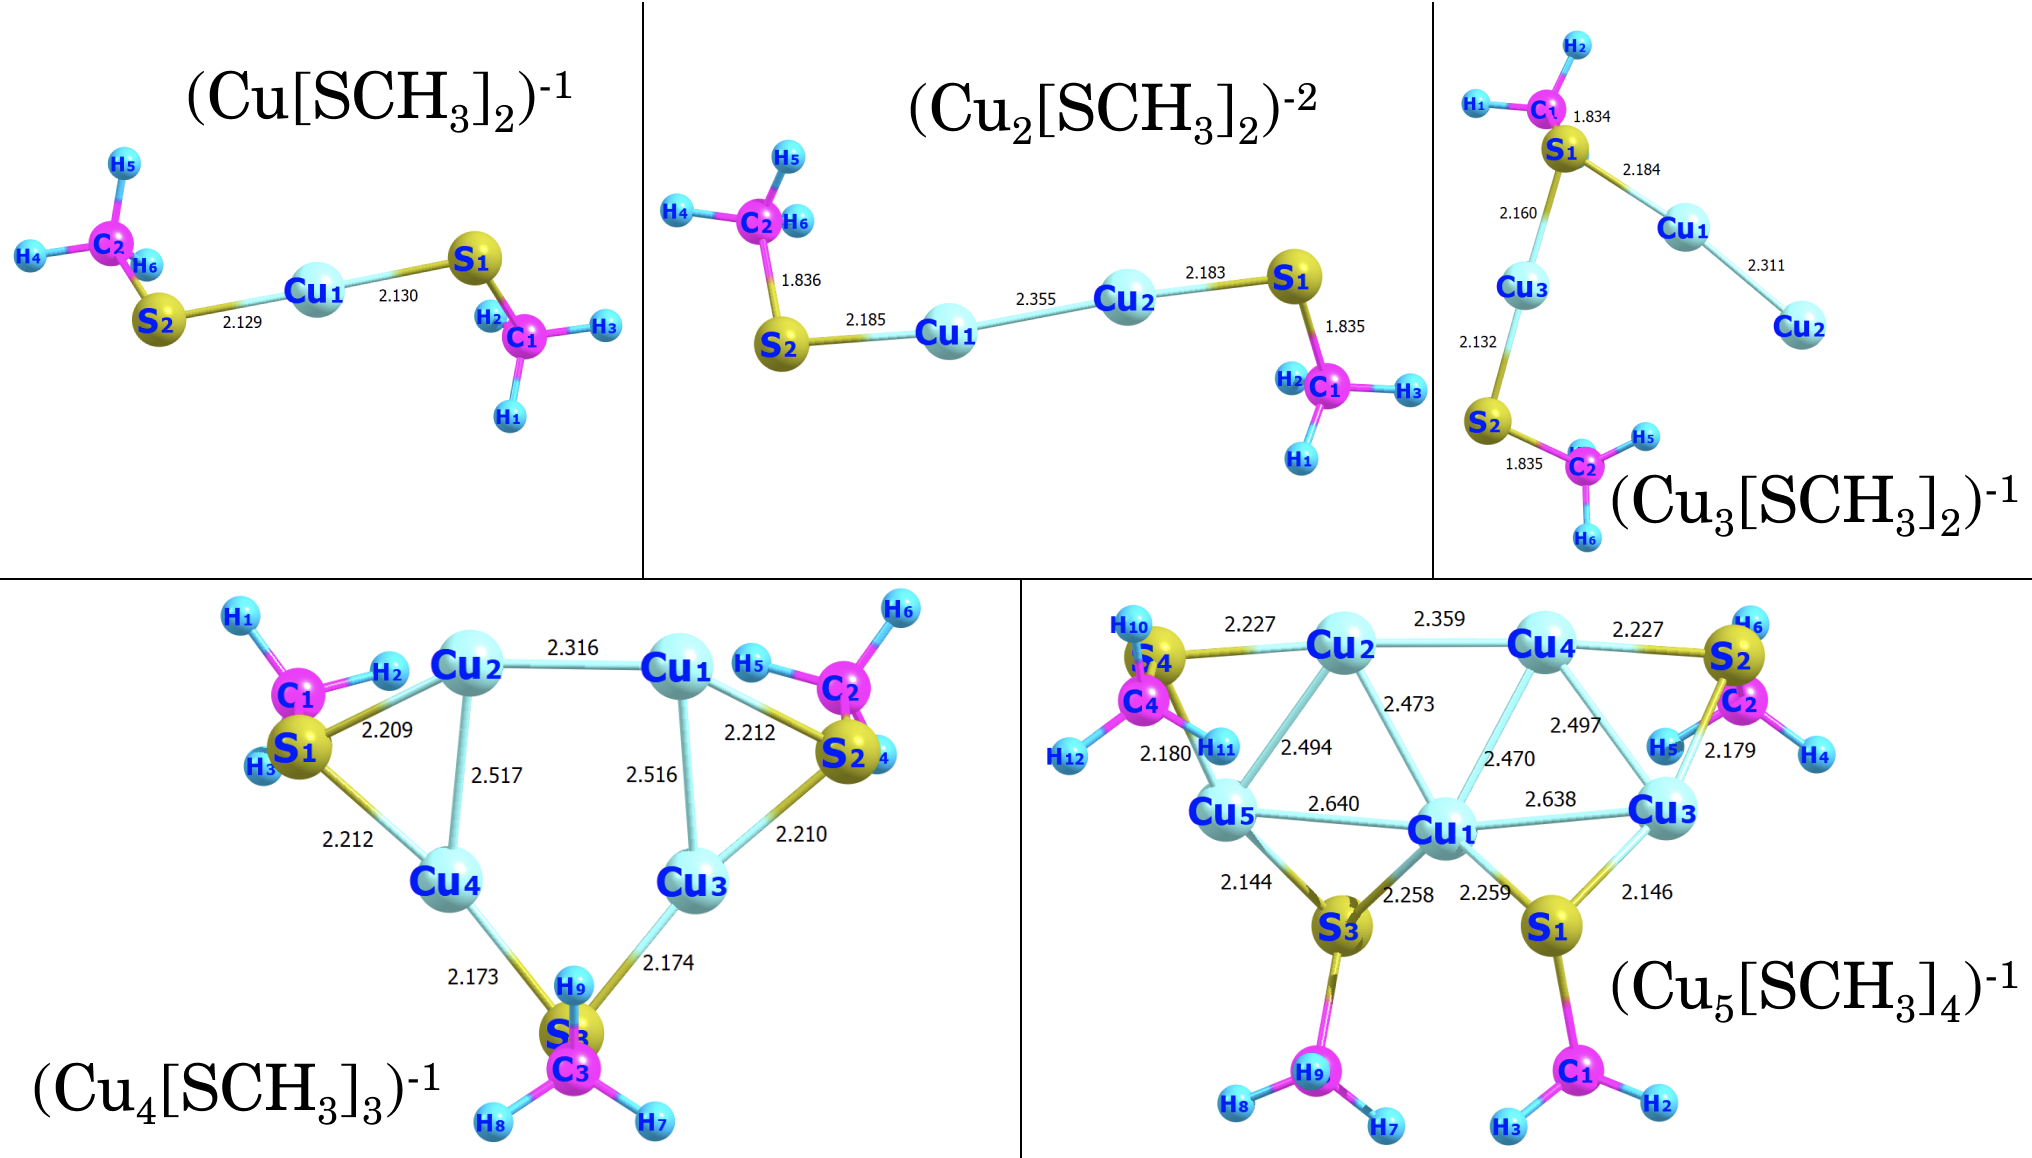
\includegraphics[width=0.8\textwidth, frame]{pictures/opt_SCH3_wat.jpg}
		%		\caption{Оптимизированные {в воде} геометрии комплексов,стабилизированных метилтиогруппой (метод: MP2 def2-TZVP.}
		%		\label{fig_geoopt_SCH3_wat}
		%	\end{figure}
	
	Обобщая сказанное, полученные в воде и газовой фазе результаты в ряде случаев значительно отличаются друг от друга. Вероятнее всего, это обосновывается особенностями континуальной модели CPCM. Это искажение равновесной геометрии в воде может в значительной мере влиять на характер спектров поглощения и люминесценции. Полученные оптимизированные структуры данных комплексов в дальнейшем были использованы для расчёта спектров поглощения.
	
	\subsubsection*{Спектры поглощения комплексов}
	% \addcontentsline{toc}{subsubsection}{Спектры поглощения комплексов}
	
	Модельные спектры поглощения получены при помощи пяти DFT функционалов: BHandHLYP, CAM-B3LYP, M06-2X, PBE0 и wB97X. Для BHandHLYP, CAM-B3LYP и PBE0 использована поправка D3 на дисперсионные взаимодействия с демпфирующей функцией Беке-Джонсона \cite{Grimme2011}. Для функционала M06-2X эта поправка недоступна, поэтому она была заменена на D3zero, с оригинальной демпфирующей функцией Гримме \cite{Grimme2010}. В случае с wB97X, никакой дисперсионной поправки использовано не было, так как она уже учтена в самом функционале. 
	
	%	Нетрудно заметить, что полученные результаты сильно отличаются друг от друга. Рассмотрим для начала спектры, смоделированные при помощи функционала M06-2X, являющимся в настоящее время наиболее популярным для расчёта органо-металлических систем. Ранее было отмечено, что исходя из экспериментальных данных (масс-спектрометрии), наиболее часто в растворе встречаются комплексы с двухатомным кластером и ионом меди (см. Рис.\ths\ref{fig_cu_mass_spec}). И действительно, на Рис.\ths\ref{fig_abs_functionals}\ths(c) мы видим, что рассчитанный вакууме спектр \ce{[Cu2(SCH3)2]^{-2}} очень хорошо приближает экспериментальный. Комплекс \ce{[Cu(SCH3)2]^{-1}} в исследуемой области не поглощает, что явно видно на Рис.\ths\ref{fig_abs_complexes}\ths(a) (самый длинноволновый переход на длине волны порядка 270 нм).
	
	%	Можно предположить, что в растворе также присутствует некоторое количество комплекса с трёхатомным кластером, исходя из расчётов. На Рис.\ths\ref{fig_abs_functionals}\ths(c) видно, что все остальные спектры имеют смещённые, относительно экспериментального спектра, максимумы поглощения. 
	
	В качестве референса использован спектр поглощения, рассчитанный при помощи метода связанных кластеров CCSD. Бенчмаркинг проводился на основе данных, полученных для пяти комплексов меди. Полученные результаты приведены на Рис. \ref{fig_bench_Cu_vac}–\ref{fig_bench_Cu5_vac}.
	
	В случае с одноатомным кластером, почти все методы дали переходы в коротковолновой области, которых нет в методе связанных кластеров. Лучше всего спектр, полученный при помощи CCSD, сходится с спектром, полученным при помощи функционала CAM-B3LYP. Результаты, полученные методом M06-2X также неплохо согласуются с CCSD, однако значительно хуже по сравнению с методом CAM-B3LYP.  
	
	\begin{figure}[H]
		\centering
		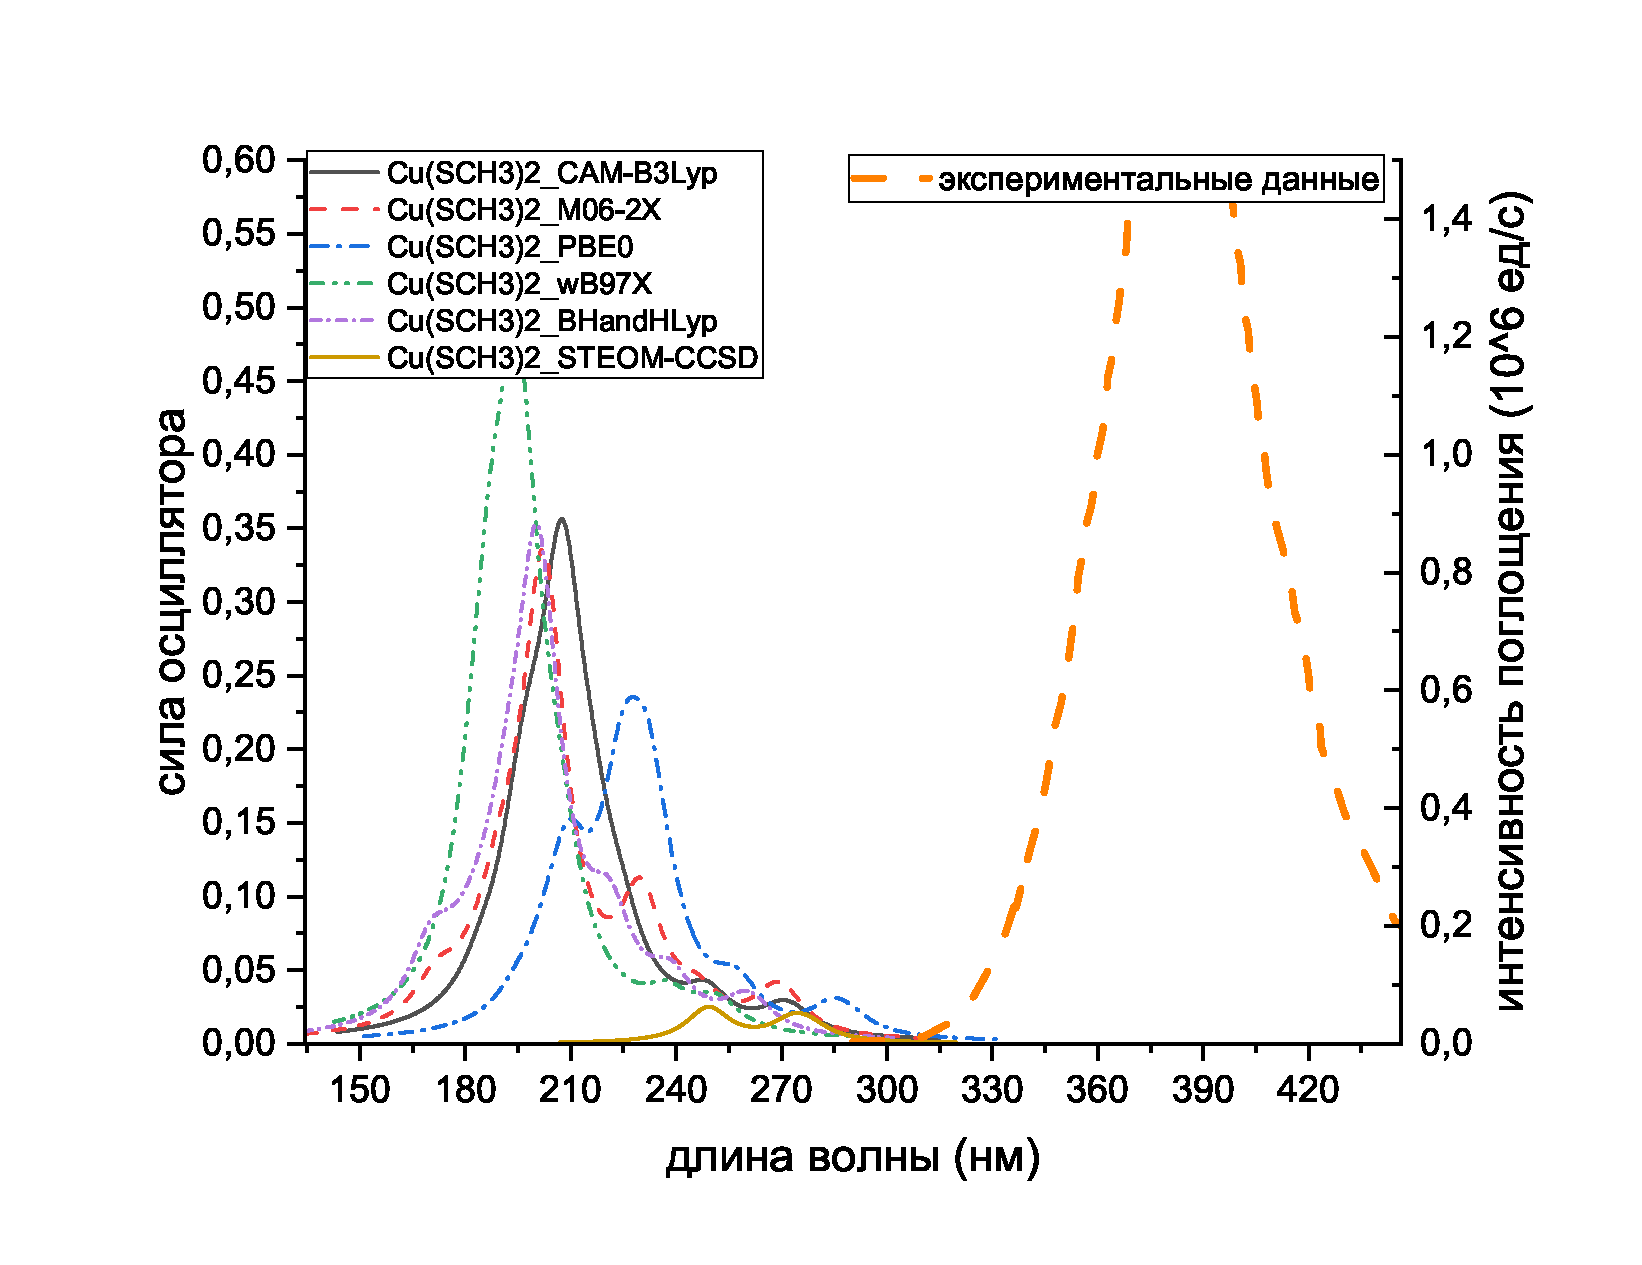
\includegraphics[width=0.8\textwidth]{pictures/spectra/Cu_vacuum.eps}
		\caption{Рассчитанные спектры поглощения для комплекса \ce{[Cu(SCH3)2]^{-1}} в газовой фазе. Использовано Лоренцево уширение с полушириной 15нм.}
		\label{fig_bench_Cu_vac}
	\end{figure}
	
	\begin{figure}[H]
		\centering
		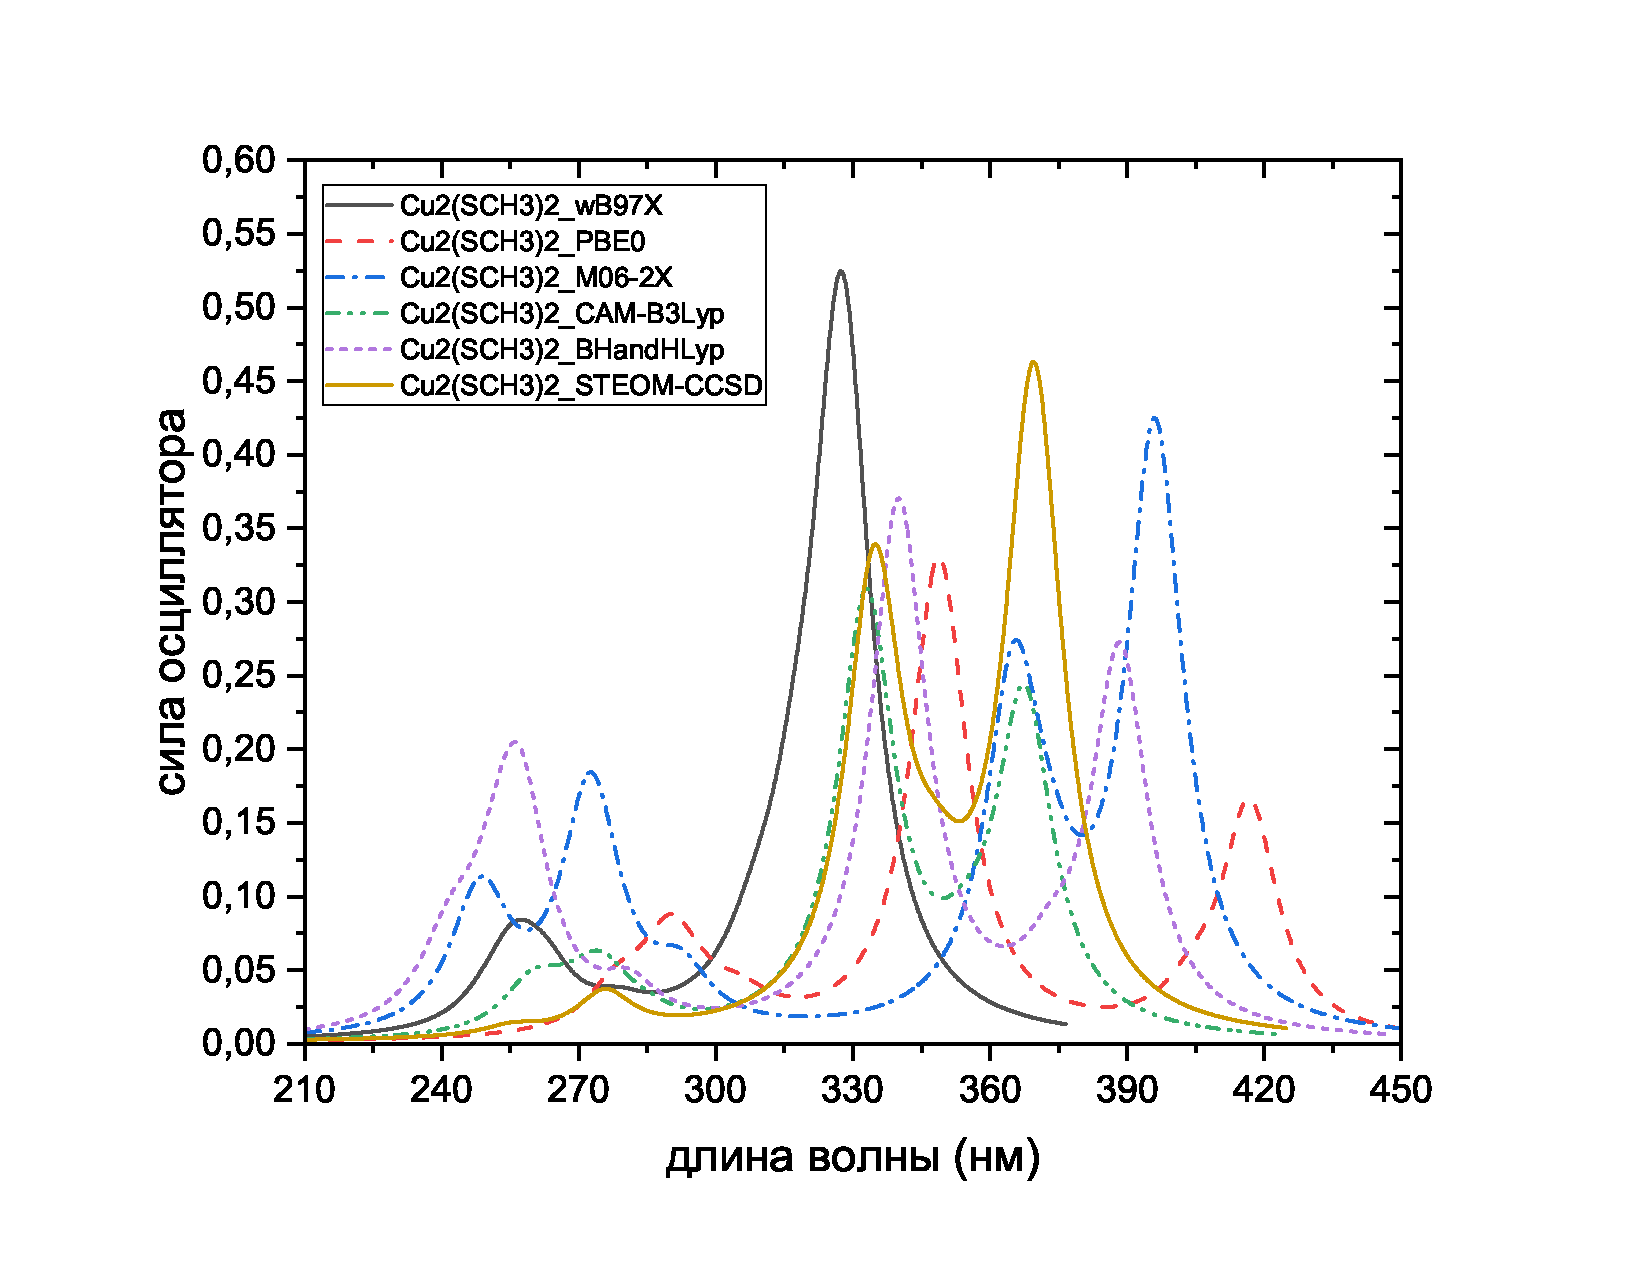
\includegraphics[width=0.8\textwidth]{pictures/spectra/Cu2_vacuum.eps} 
		\caption{Рассчитанные спектры поглощения для комплекса \ce{[Cu2(SCH3)2]^{-2}} в газовой фазе. Использовано Лоренцево уширение с полушириной 15нм.}
		\label{fig_bench_Cu2_vac}
	\end{figure}
	
	Для двухатомного кластера наблюдается похожая картина: переходы, полученные с использованием функционала CAM-B3LYP в наибольшей степени согласуются с методом связанных кластеров. Второе место по точности занимает функционал M06-2X. Для него оба перехода получились смещёнными на 40 нм в длинноволновую область, однако форма спектральных линий почти точь-в-точь совпадает с спектром, полученным при помощи CCSD.
	
	Спектры, полученные для комплекса с трёхатомным кластером, сравнительно плохо согласуются с экспериментальным. Форма спектральной линии для методов BHandH-LYP и M06-2X практически идеально согласуется с референсным спектром. Остальные функционалы дают смещённый в длинноволновую область главный переход и дополнительные переходы в коротковолновой области.
	
	Для комплекса \ce{[Cu4(SCH3)3]^{-1}} наблюдается сильный разброс спектров как по энергиям, так и по интенсивностям. Лучшую сходимость с методом связанных кластеров в этом случае дал функционал PBE0, для которого энергии основных электронных переходов отклоняются от CCSD спектра не более, чем на 5нм. 
	
	Наконец, для пятиатомного кластера меди ни один спектр, полученный при помощи DFT функционалов, не совпал хорошо с CCSD. По форме все спектры достаточно схожи между собой, однако на форму спектральной линии поглощения, полученной экспериментально, похожи спектры BHandH-LYP, wB97X и хуже CAM-B3LYP. Остальные три спектра смещены в длинноволновую сторону. 
	
	Подробное сравнение с экспериментальным спектром поглощения будет проведено далее, однако уже сейчас можно отметить следующие закономерности:
	\begin{enumerate}
		\item Спектры поглощения комплекса \ce{[Cu(SCH3)2]^{-1}} , полученные всеми методами лежат в коротковолновой области относительно экспериментального, что явно видно из Рис. \ref{fig_bench_Cu_vac}.
		\item Спектр, полученный при помощи функционала M06-2X для двухатомного кластера практически идеально совпадает с экспериментальным (см. Рис. \ref{fig_bench_Cu2_vac}). Это замечание можно списать на совпадение, однако масс-спектрометрия также показала наличие большого количества комплекса \ce{[Cu2(SCH3)2]^{-2}} в растворе (см. Рис. \ref{fig_cu_mass_spec}).
	\end{enumerate}
	
	\begin{figure}[H]
		\centering
		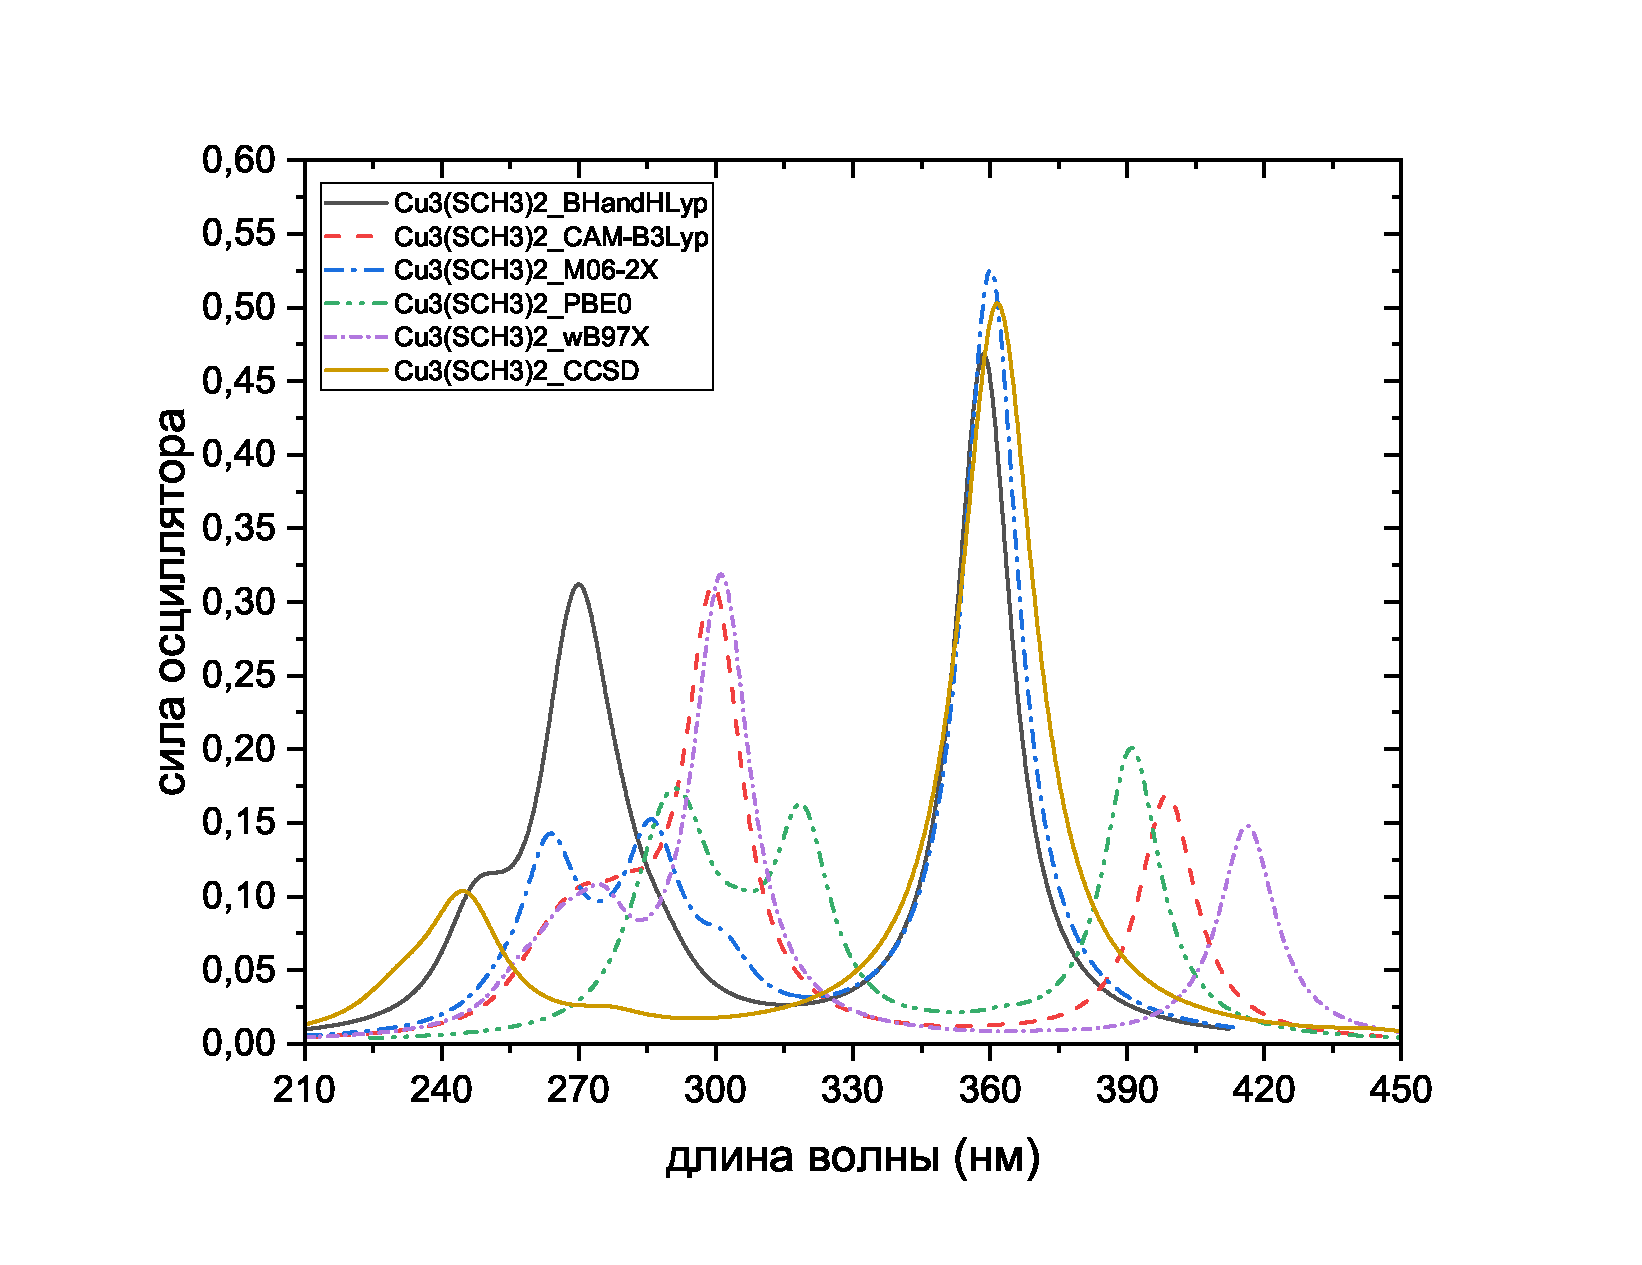
\includegraphics[width=0.8\textwidth]{pictures/spectra/Cu3_vacuum.eps}
		\caption{Рассчитанные спектры поглощения для комплекса \ce{[Cu3(SCH3)2]^{-1}} в газовой фазе. Использовано Лоренцево уширение с полушириной 15нм.}
		\label{fig_bench_Cu3_vac}
	\end{figure}
	
	\begin{figure}[H]
		\centering
		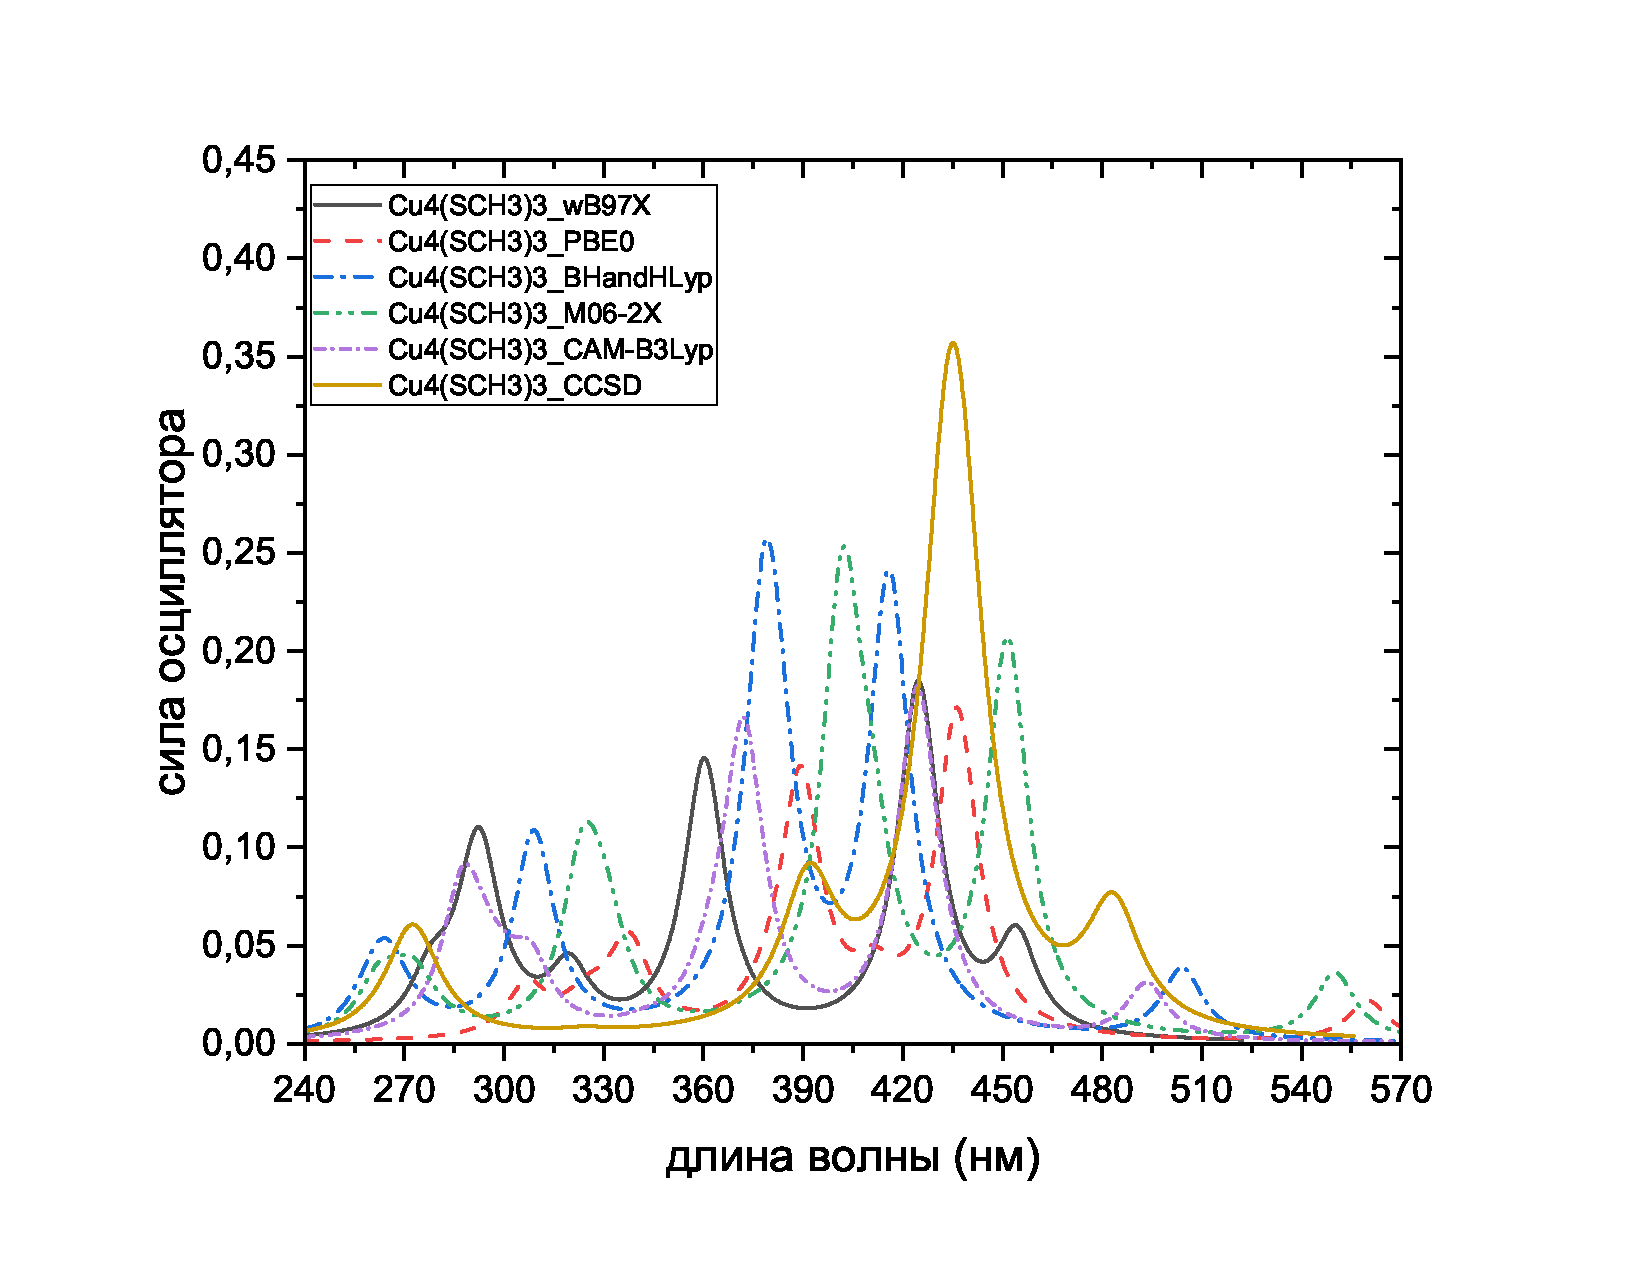
\includegraphics[width=0.8\textwidth]{pictures/spectra/Cu4_vacuum.eps} 
		\caption{Рассчитанные спектры поглощения для комплекса \ce{[Cu4(SCH3)3]^{-1}} в газовой фазе. Использовано Лоренцево уширение с полушириной 15нм.}
		\label{fig_bench_Cu4_vac}
	\end{figure}
	
	\begin{figure}[H]
		\centering
		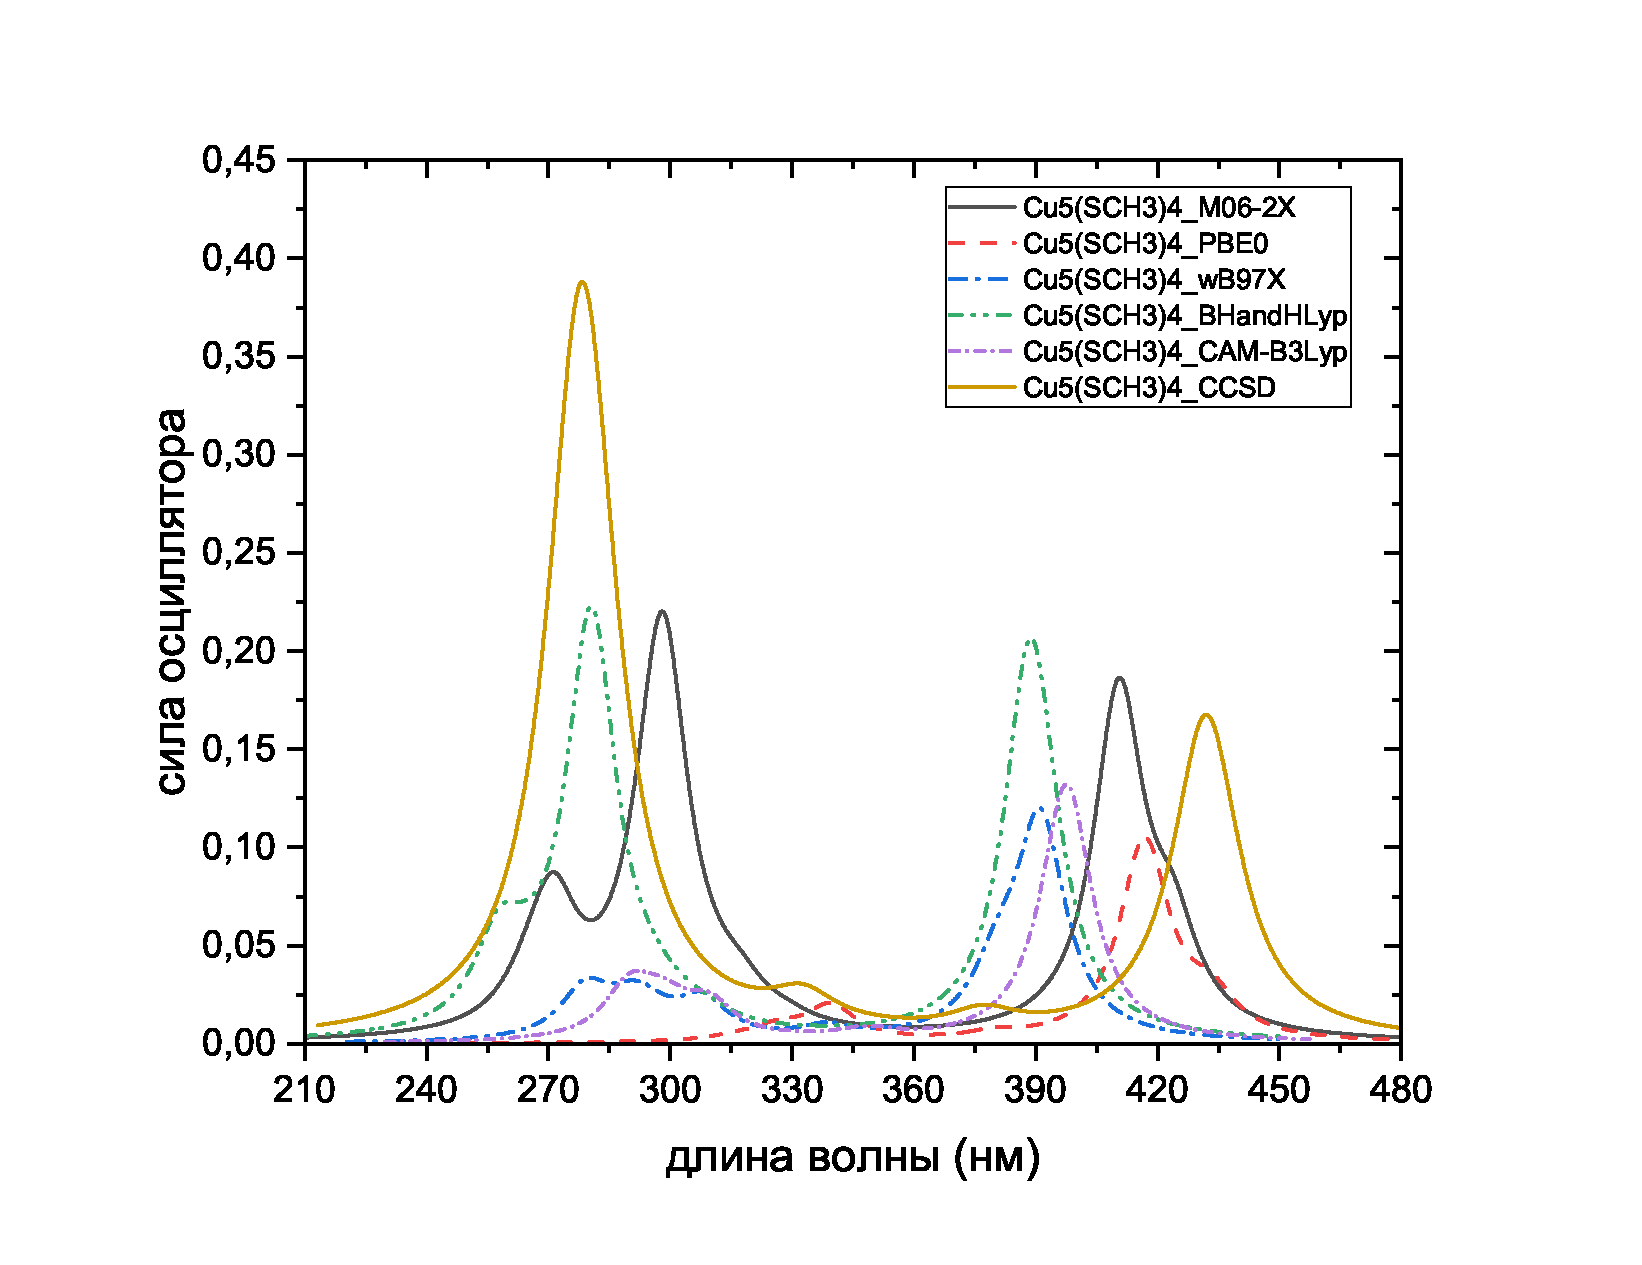
\includegraphics[width=0.8\textwidth]{pictures/spectra/Cu5_vacuum.eps}
		\caption{Рассчитанные спектры поглощения для комплекса \ce{[Cu5(SCH3)4]^{-1}} в газовой фазе. Использовано Лоренцево уширение с полушириной 15нм.}
		\label{fig_bench_Cu5_vac}
	\end{figure}
	
	Для всех комплексов посчитаны среднеквадратичные разности DFT и CCSD энергий для соответствующих переходов. Также отдельно посчитанно RMSE для первого перехода (обычно, HOMO$\rarr$LUMO), в силу особого интереса к этой характеристике. Полученные результаты представлены в Табл.\ths\ref{tab_bench_1} и Табл.\ths\ref{tab_bench_2}.
	
	\begin{table}[H]
		\caption{Среднеквадратичная разность CCSD–DFT для всех переходов в эВ.}
		\label{tab_bench_1}
		\centering
		\begin{tabular}{|c|c|c|c|c|c|c|}
			\hline
			BHandH-LYP	&	CAM-B3LYP	& M06-2X	& PBE0	& wB97X		 \\ \hline
			1,68				 &   1,05					& 1,39			 & 1,42		& 1,75			 \\ \hline
		\end{tabular}
	\end{table}
	
	\begin{table}[H]
		\caption{Среднеквадратичная разность CCSD–DFT для HOMO-LUMO переходов в эВ.}
		\label{tab_bench_2}
		\centering
		\begin{tabular}{|c|c|c|c|c|c|c|}
			\hline
			BHandH-LYP	&	CAM-B3LYP	& M06-2X	& PBE0	& wB97X 	\\ \hline
			0,45				 &   0,37					& 0,48			& 0,68	 & 0,79 		 \\ \hline
		\end{tabular}
	\end{table}	
	
	Из полученных выше результатов можно заключить, что лучше всего с высокоуровневым методом связанных кластеров согласуется DFT функционал CAM-B3LYP. Расчёты, полученные при помощи функционала M06-2X сильнее отличаются от CCSD спектра, однако лучше согласуются с экспериментальными данными. При этом по точности он занимает второе место. Худшие результаты показал функционал WB97X. Примечательно, что PBE0 оказался в среднем лучше BHandH-LYP, однако для расчёта длинноволнового перехода первый функционал лучше сходится CCSD.
	
	На Рис. \ref{fig_abs_CAM-B3LYP_vac} и \ref{fig_abs_M06-2X_vac} приведены спектры поглощения всех комплексов в газовой фазе, полученные при помощи функционалов CAM-B3LYP и M06-2X соответственно.	Нетрудно заметить, что ни один из спектров поглощения, рассчитанных при помощи функционала CAM-B3LYP, не согласуется хорошо с экспериментом: для иона меди (как и в случае с другими функционалами) спектр лежит значительно в более коротковолновой области, нежели экспериментальный; спектр комплекса с двухатомным кластером меди опять же лежит сильно левее экспериментального (смещение приблизительно на 40нм в коротковолновую область, с учётом уширения). Трёхатомный комплекс является хорошим кандидатом на присутствие в растворе, однако сильное поглощение в коротковолновой области сразу отвергает его кандидатуру. Спектр пятиатомного кластера похож на спектр трёхатомного, однако без поглощения в коротковолновой области; он мог бы быть наиболее вероятно встречающимся в растворе, если бы не максимум поглощения, смещённый приблизительно на 15нм в длинноволновую область. Форма спектра поглощения комплекса с четырёхатомным кластером меди значительно отличается от экспериментального. 
	
	\begin{figure}[!h]
		\centering
		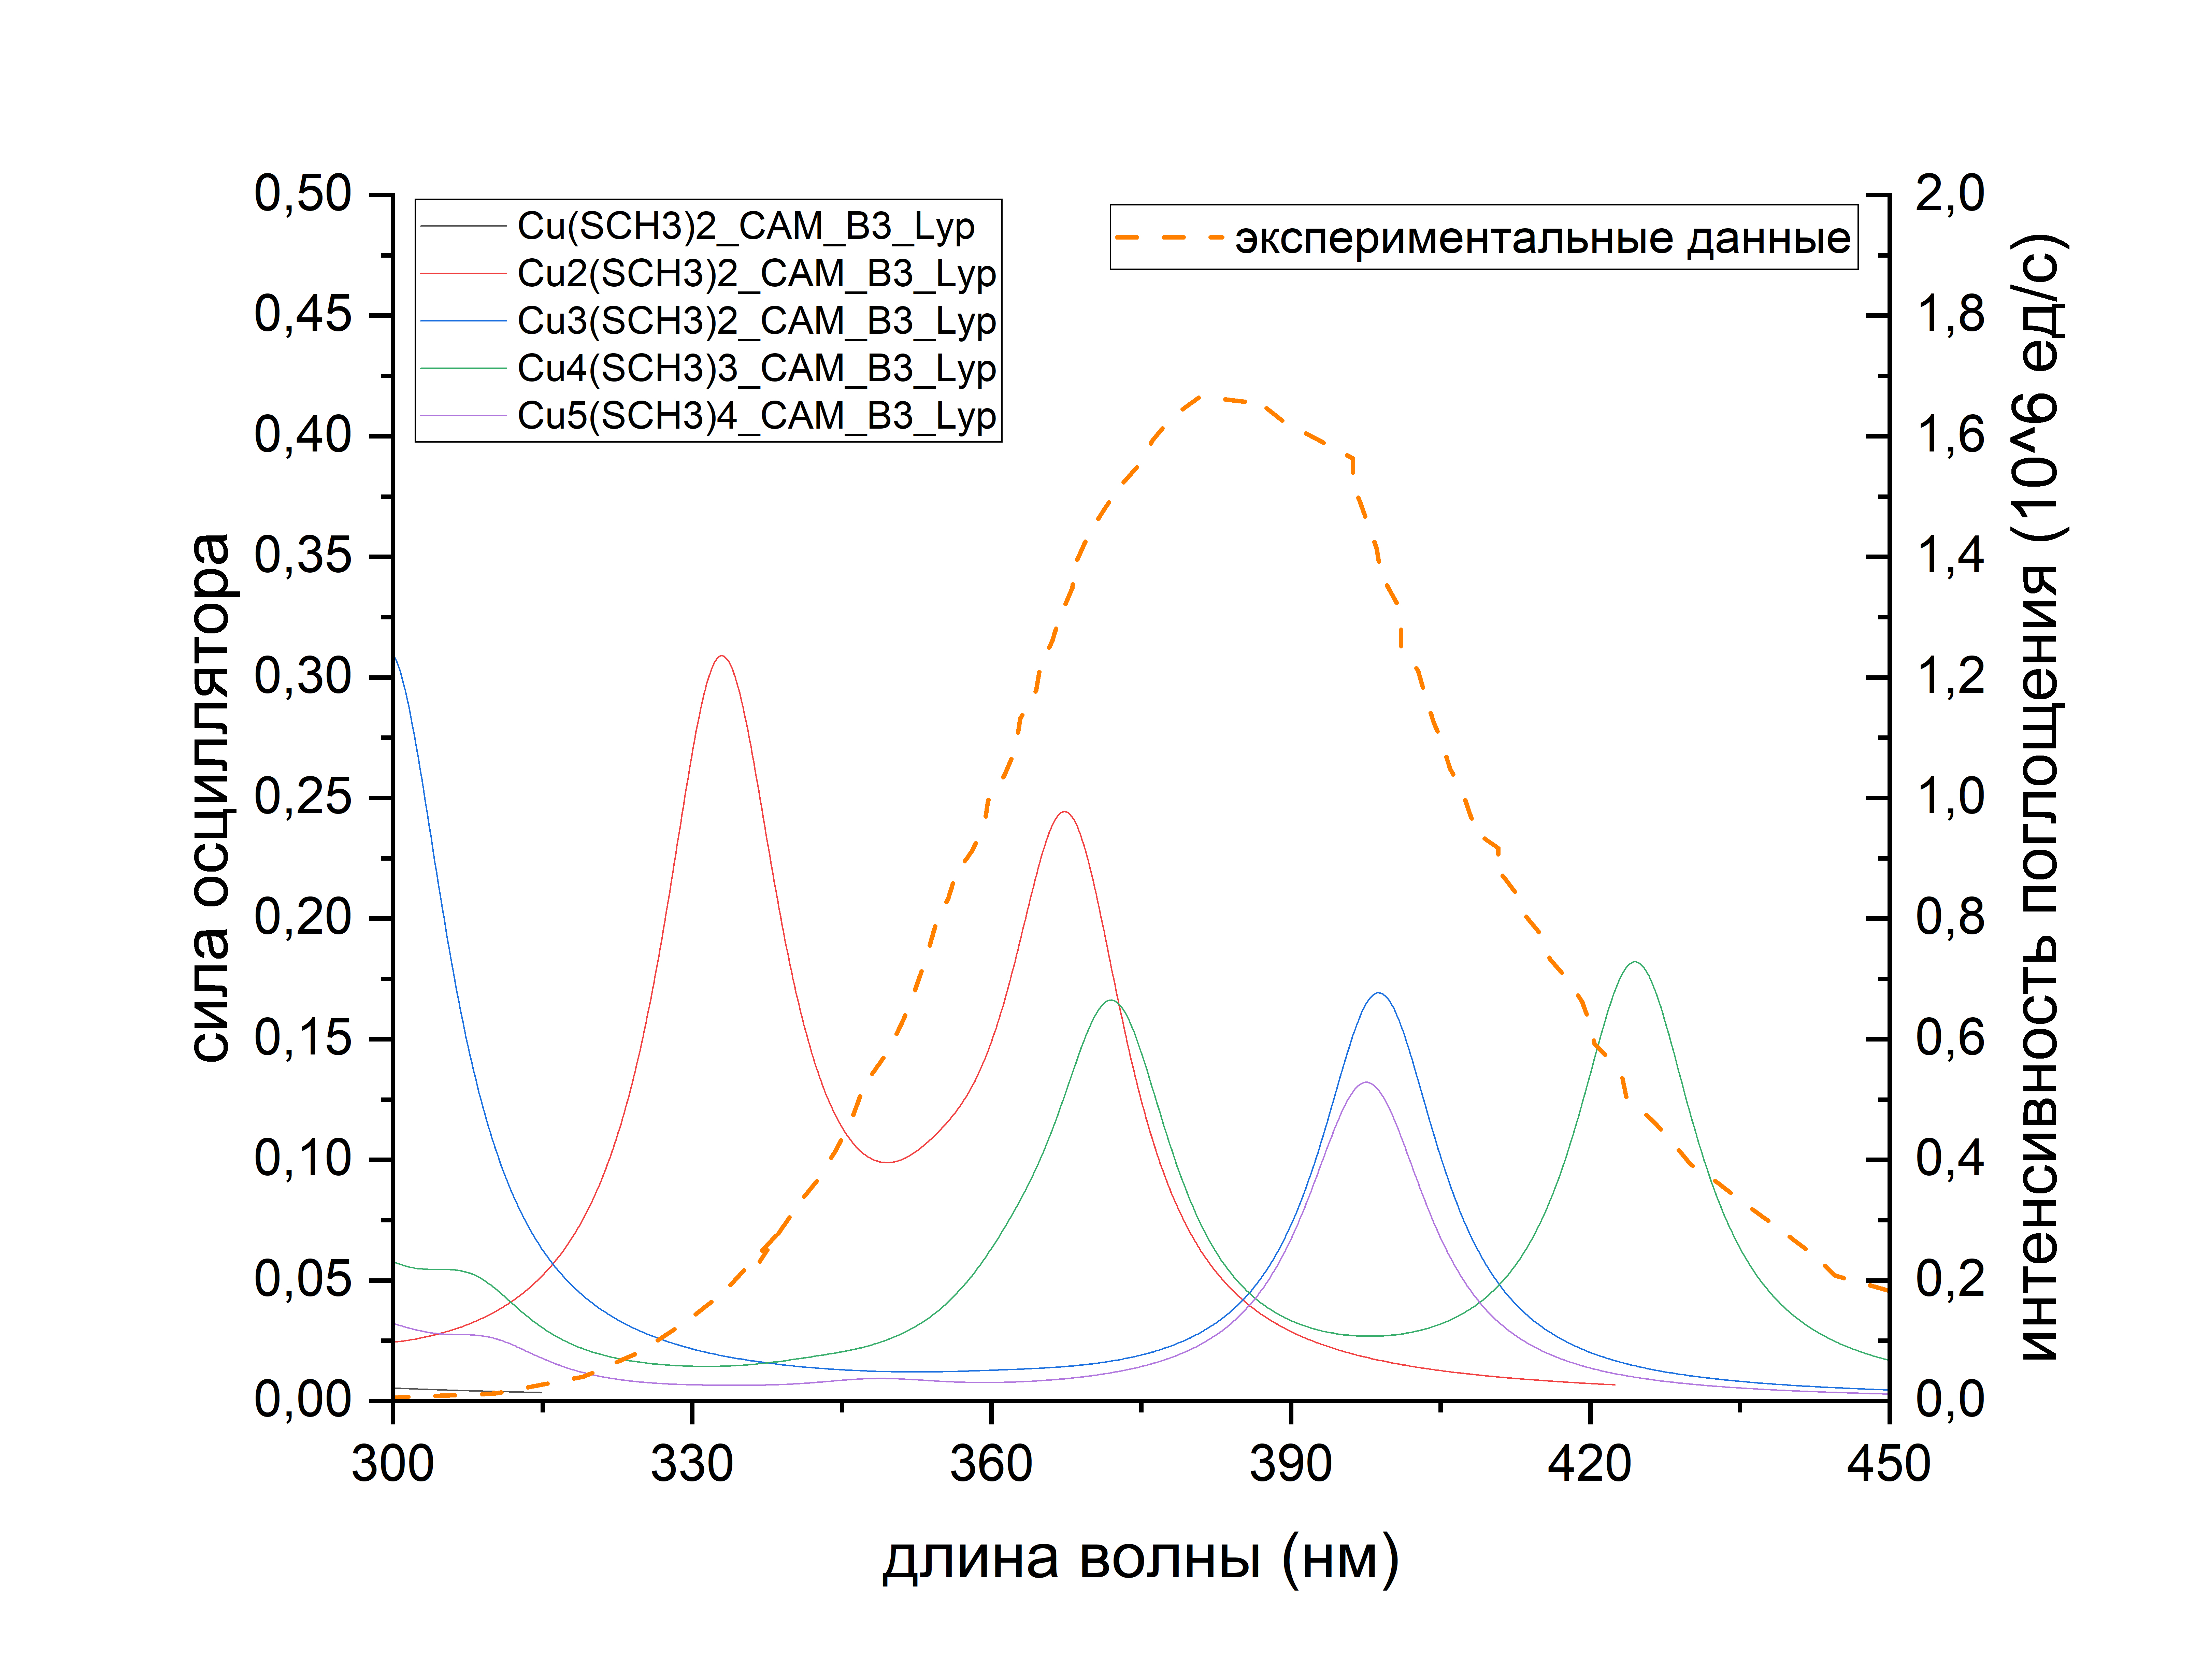
\includegraphics[width=0.8\textwidth]{pictures/spectra/CAM-B3Lyp.jpg}
		\caption{Модельные спектры поглощения комплексов с метилтиогруппой, полученные при помощи функционала CAM-B3LYP в газовой фазе. Использовано Лоренцево уширение с полушириной 15нм.}
		\label{fig_abs_CAM-B3LYP_vac}
	\end{figure}
	
	\begin{figure}[H]
		\centering
		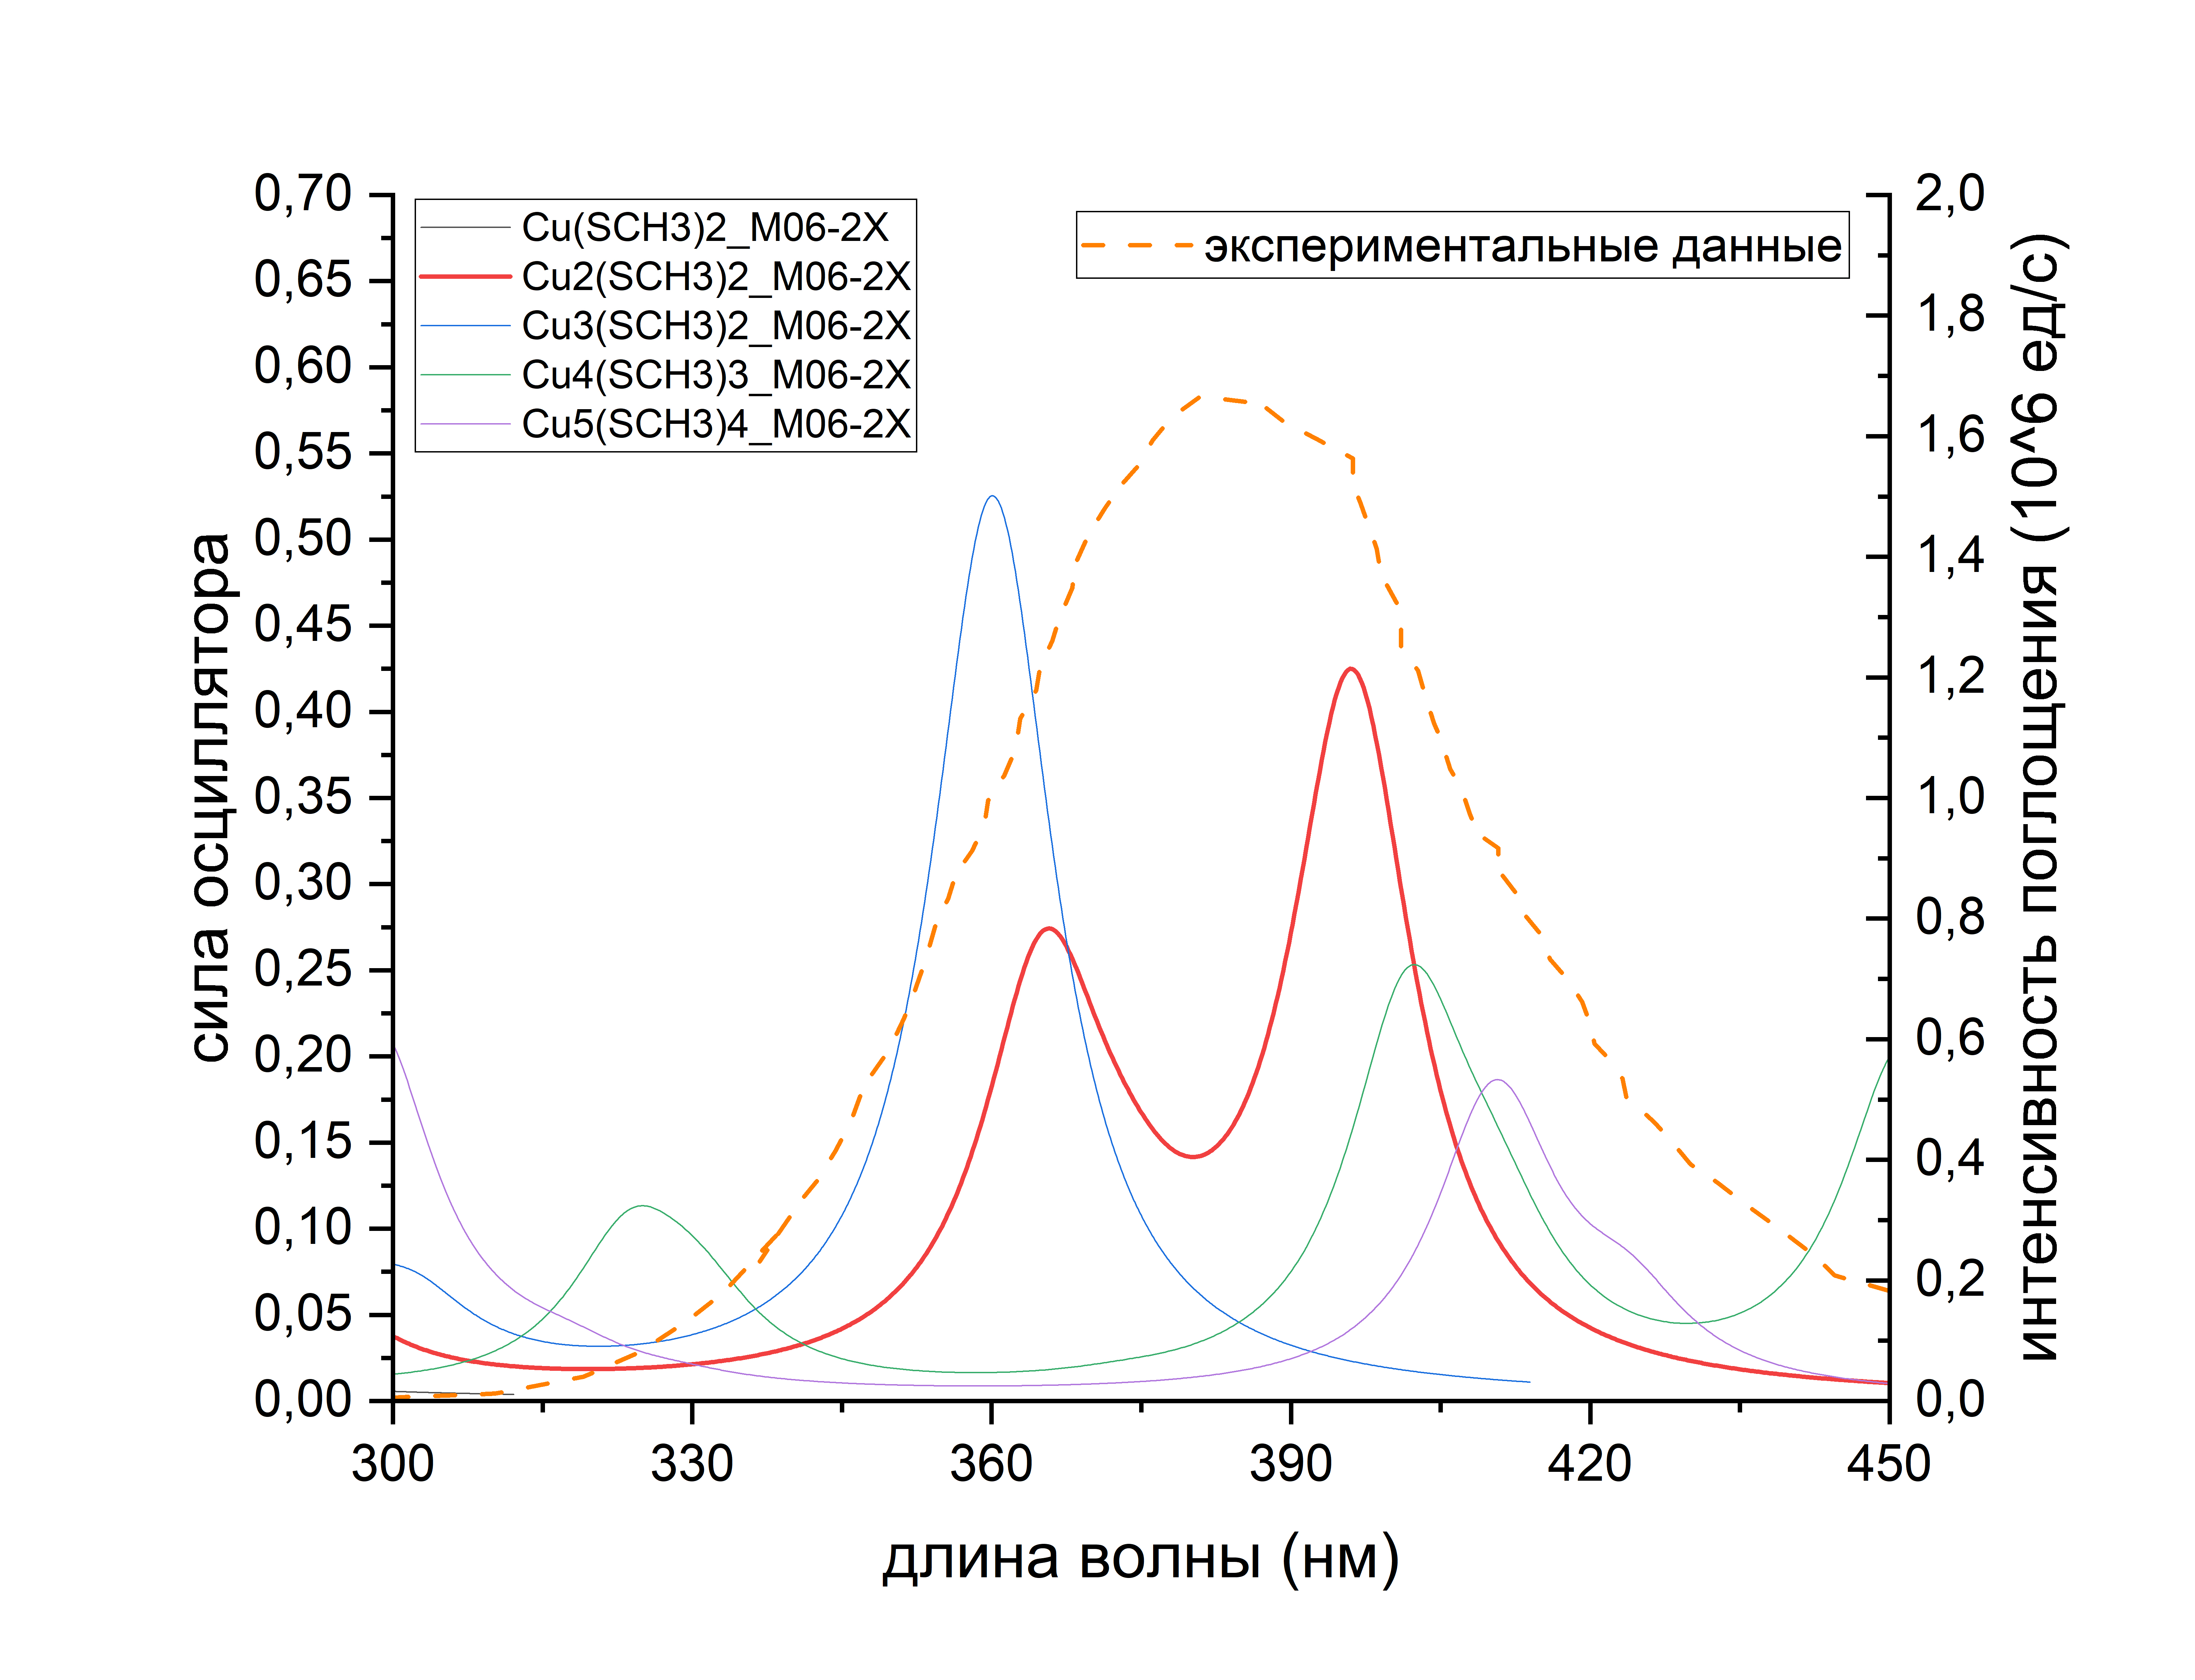
\includegraphics[width=0.8\textwidth]{pictures/spectra/M06-2X.jpg} 
		\caption{Модельные спектры поглощения комплексов с метилтиогруппой, полученные при помощи функционала M06-2X в газовой фазе. Использовано Лоренцево уширение с полушириной 15нм.}
		\label{fig_abs_M06-2X_vac}
	\end{figure}
	
	Рассматривая спектры поглощения комплексов, рассчитанные методом M06-2X, можно заметить следующие закономерности: комплекс \ce{[Cu2(SCH3)2]^{-2}} поглощает практически в точности как и экспериментальный раствор, однако немного отличается от него так как, в реальном растворе присутствует также некоторое количество других комплексов. Форма экспериментального спектра говорит о наличии некоторого поглощающего соединения на длине волны около 400нм. Под этот критерий попадают комплексы с чтырёхатомным и пятиатомным кластерами меди; можно предположить, что в эксперименте наблюдается влияние именно \ce{[Cu4(SCH3)3]^{-1}}, из-за наличия поглощения в длинноволновой области. Помимо этого, в растворе может присутствовать некоторое количество комплекса с трёхатомным кластером, пик интенсивности поглощения которого лежит в более коротковолновой области относительно максимума поглощения экспериментального раствора.
	
	Обобщая сказанное, в случае с функционалом CAM-B3LYP ни один из модельных спектров не согласуется хорошо с экспериментальным; результаты, полученные с использованием функционала M06-2X сильно лучше согласуются с экспериментом, в частности спектр поглощения комплекса с двухатомным кластером меди практически идеально согласуется с экспериментальным. 
	
	Примечательно, что лучшие результаты были получены с использованием функционалов с 54\% ХФ вкладом (M06-2X) и вариативным, от 19\% на малых до 65\% на длинных, ХФ вкладом (CAM-B3LYP).
	
	Проанализируем энергетическую структуру двухатомного кластера. Основные электронные переходы, соответствующие линиям поглощения комплекса, представлены на Рис. \ref{fig_elect_trans}:
	
		\begin{figure}[!htb]
				\centering
				
				\subfloat[Переход 2px \rarr 2py]{ 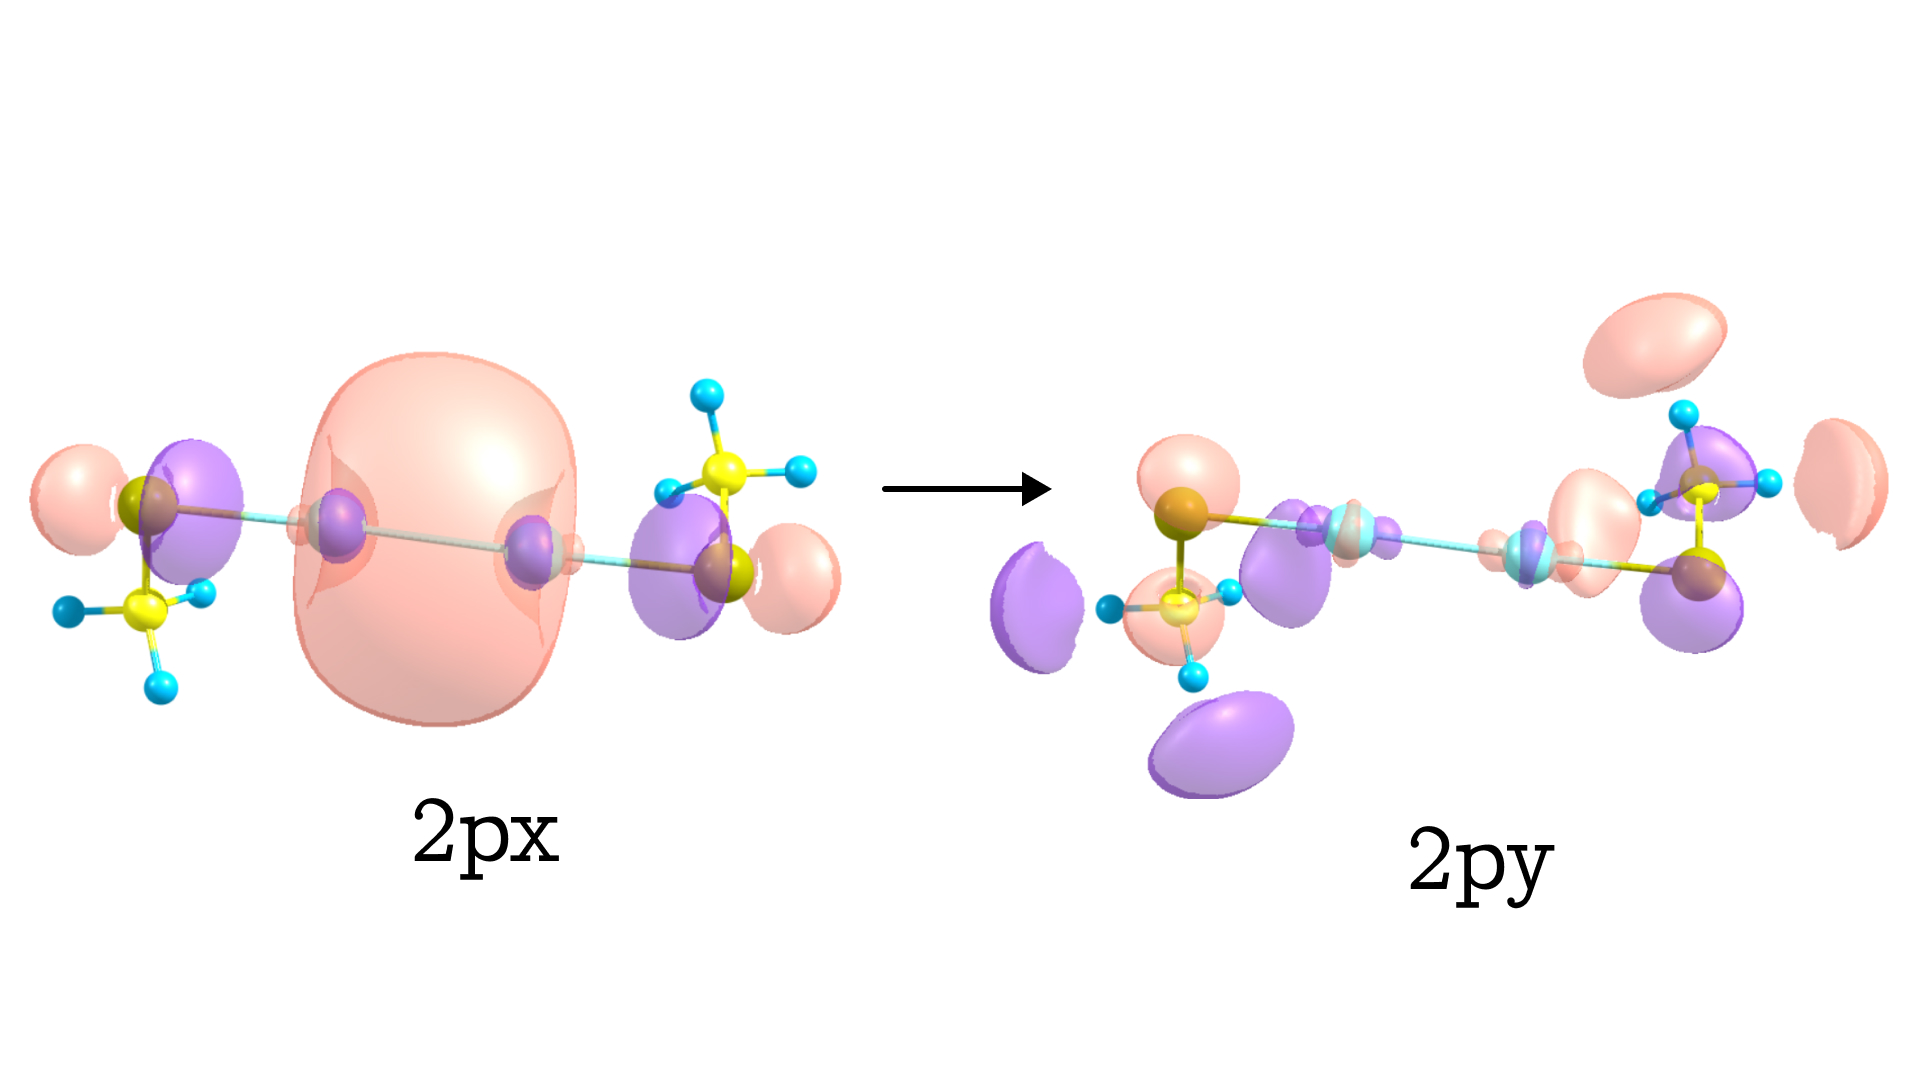
\includegraphics[clip,width=0.33\columnwidth]{figures/orbitals/Cu2L2_1.jpg} }
				\subfloat[Переход 2px \rarr 3pz]{ 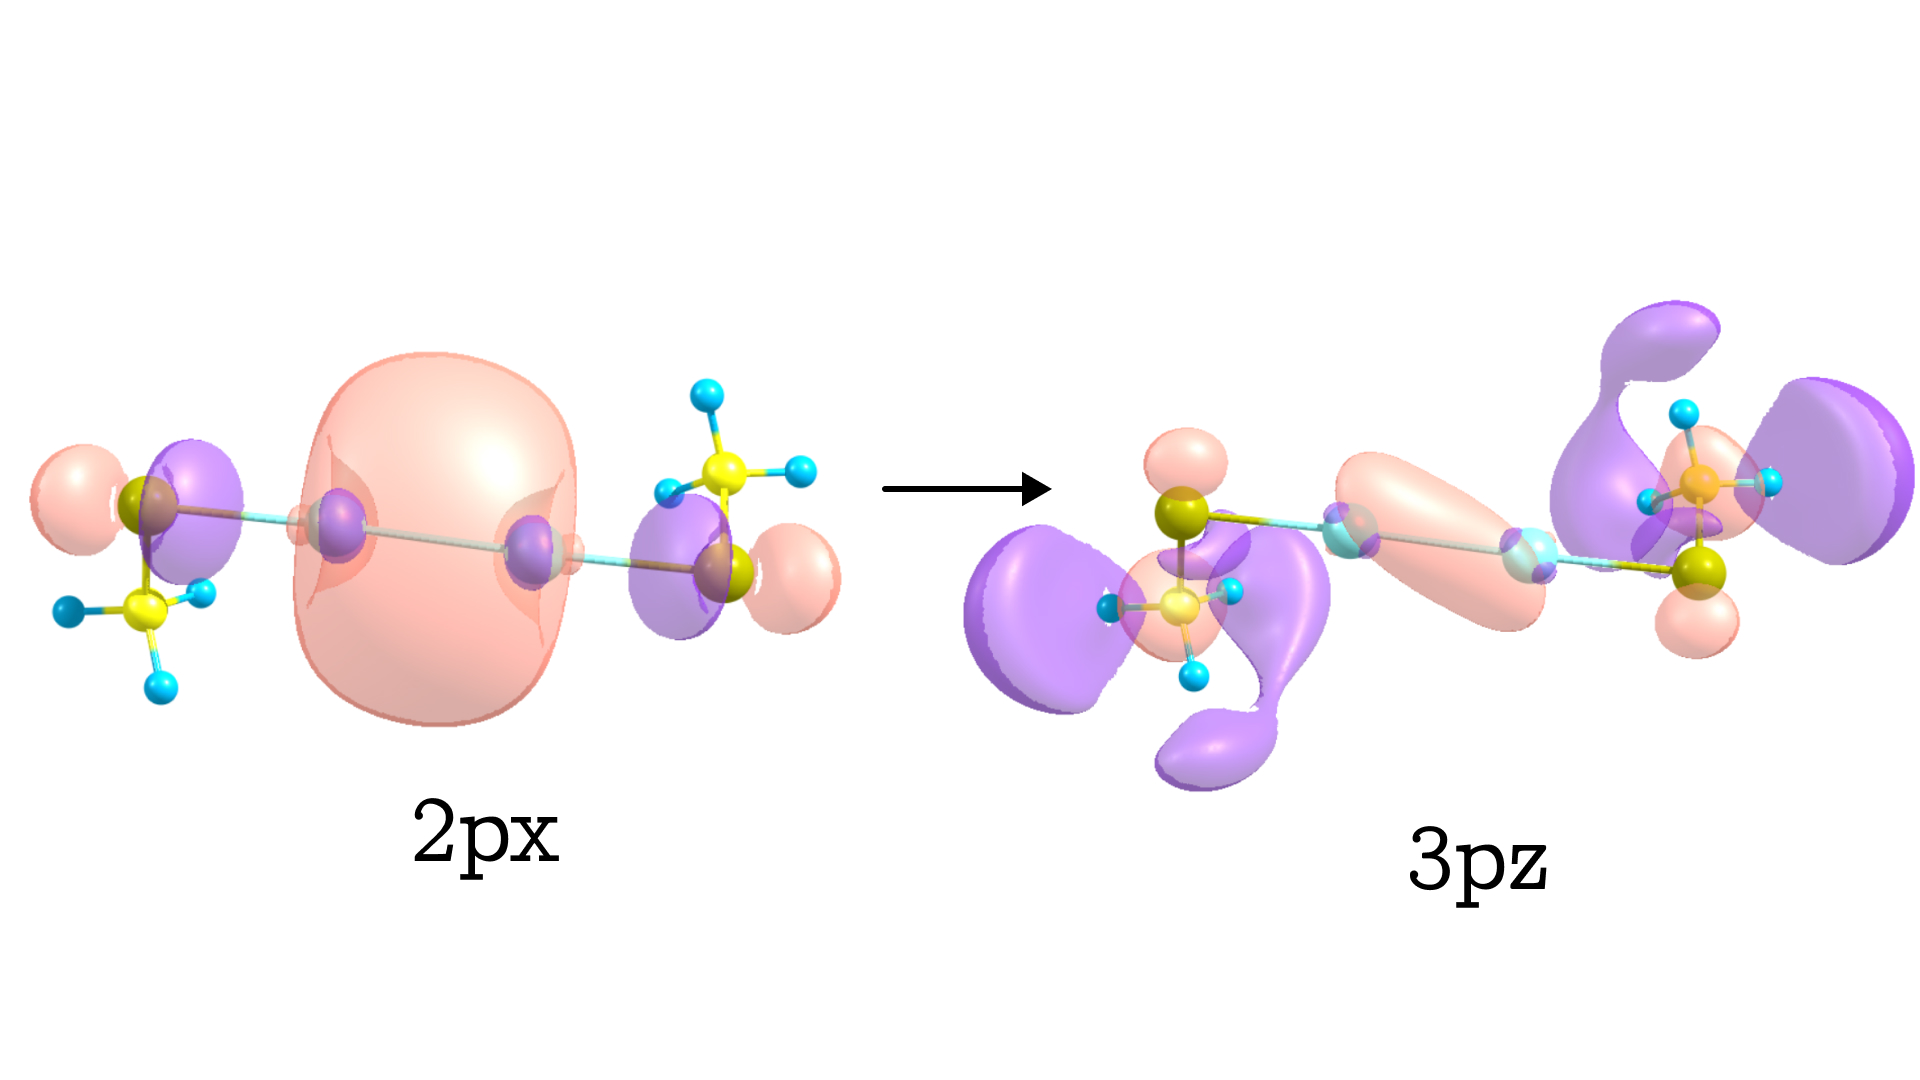
\includegraphics[clip,width=0.33\columnwidth]{figures/orbitals/Cu2L2_2.jpg} }
				\subfloat[Переход 2px \rarr 3px]{ 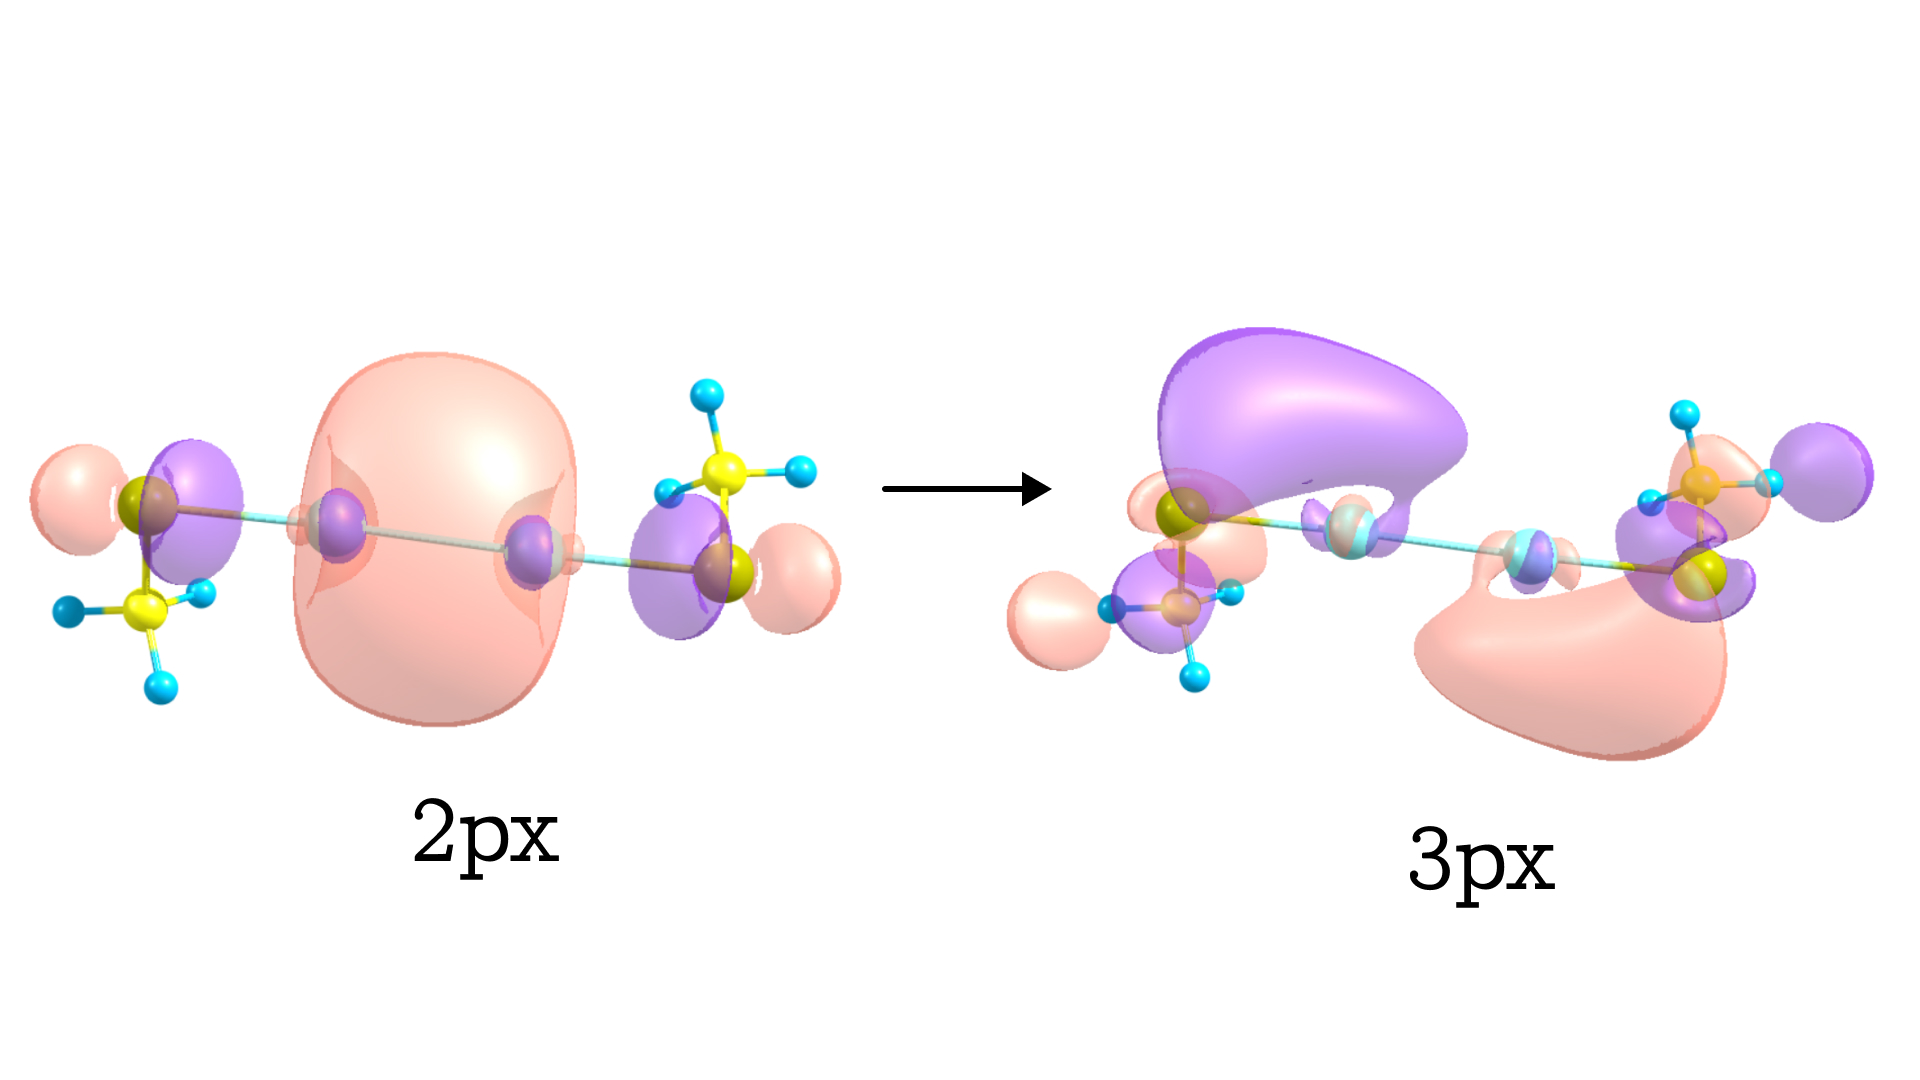
\includegraphics[clip,width=0.33\columnwidth]{figures/orbitals/Cu2L2_3.jpg} }
				
				\caption{Основные вклады в спектр поглощения комплекса \ce{[Cu2(SCH3)2]^{-2}} в газовой фазе. Проекция изоповерхностей модельной электронной плотности. Метод def2-TZVP/M06-2X.}
				\label{fig_elect_trans}
			\end{figure}
		
		Проведём сравнительный анализ результатов, полученных разными методами для комплекса \ce{[Cu2(SCH3)2]^{-2}}. В таблице \ref{tab7} приведены силы осцилляторов, длины волн и электронные орбитали, между которыми происходит  переход.  
		
		Во всех случаях прослеживается общая тенденция:  доминирующими являются первый и третий переход, а сила осциллятора для второго является сравнительно малой. Исключением является wB97X, для которого силы осцилляторов второго и третьего переходов сравнимы друг с другом и много меньше первого. Интенсивности, при этом, могут по-разному соотноситься между собой: для функционалов M06-2X и wB97X самый длинноволновый переход имеет большую силу осциллятора, чем третий; для остальных функционалов результат противоположный, однако по абсолютной величине интенсивности различаются не так сильно. Также можно сказать, что в случае с функционалом CAM-B3LYP третий переход имеет приблизительно ту же вероятность, что и первый. 
		
		\begin{table}[H]
				\caption{Длины волн модельных электронных переходов (в нм), рассчитанных при помощи разных DFT функционалов с поправкой D3 в газовой фазе. Структура \ce{[Cu2(SCH3)2]^{-2}}.}
				\label{tab7}
				\centering
					\begin{tabular}{|c|cc|cc|cc|}
					\hline
					\textbf{метод} & \multicolumn{2}{c|}{\textbf{M06-2X}}                       & \multicolumn{2}{c|}{\textbf{BHandHLYP}}                    & \multicolumn{2}{c|}{\textbf{PBE0}}                                              \\ \hline
					\textit{переход}                  & \multicolumn{1}{c|}{\textit{$\lambda$, нм}} & \textit{$f_{osc}$} & \multicolumn{1}{c|}{\textit{$\lambda$, нм}} & \textit{$f_{osc}$} & \multicolumn{1}{c|}{\textit{$\lambda$, нм}} & \textit{$f_{osc}$} \\ \hline
					HOMO $\rarr$ LUMO   & \multicolumn{1}{c|}{396,1}               & 0,4075          & \multicolumn{1}{c|}{388,4}               & 0,2578          & \multicolumn{1}{c|}{416,8}               & \multicolumn{1}{c|}{0,1573}          \\ \hline
					HOMO $\rarr$ LUMO+1 & \multicolumn{1}{c|}{373,4}               & 0,0345          & \multicolumn{1}{c|}{373,3}               & 0,0276          & \multicolumn{1}{c|}{404,3}               & \multicolumn{1}{c|}{0,0191}          \\ \hline
					HOMO $\rarr$ LUMO+2 & \multicolumn{1}{c|}{365,3}               & 0,2329          & \multicolumn{1}{c|}{340,0}               & 0,3608          & \multicolumn{1}{c|}{348,8}               & \multicolumn{1}{c|}{0,3268}          \\ \hline \hline
					\textbf{метод}& \multicolumn{2}{c|}{\textbf{CAM-B3LYP}}  & \multicolumn{2}{c|}{\textbf{wB97X}}     &   \multicolumn{2}{c|}{\textbf{STEOM-CCSD}}                                  \\ \hline
					\textit{переход}                  & \multicolumn{1}{c|}{\textit{$\lambda$, нм}} & \textit{$f_{osc}$} & \multicolumn{1}{c|}{\textit{$\lambda$, нм}} & \textit{$f_{osc}$} & \multicolumn{1}{c|}{\textit{$\lambda$, нм}} & \textit{$f_{osc}$}  \\ \hline
					HOMO $\rarr$ LUMO   & \multicolumn{1}{c|}{367,5}               & 0,2246          & \multicolumn{1}{c|}{327,6}               & 0,4941          & \multicolumn{1}{c|}{369.6}               & \multicolumn{1}{c|}{0.4445}          \\ \hline
					HOMO $\rarr$ LUMO+1 & \multicolumn{1}{c|}{354,9}               & 0,0223          & \multicolumn{1}{c|}{308,4}               & 0,0303          & \multicolumn{1}{c|}{348.2}               & \multicolumn{1}{c|}{0.0438}          \\ \hline
					HOMO$\rarr$ LUMO+2 & \multicolumn{1}{c|}{332,9}               & 0,2952          & \multicolumn{1}{c|}{317,5}               & 0,0701          & \multicolumn{1}{c|}{334.7}               & \multicolumn{1}{c|}{0.3087}          \\ \hline
				\end{tabular}
			\end{table}
		
%		Рассмотрим теперь спектры поглощения комплексов в воде, рассчитанными при помощи методов CAM-B3LYP и M06-2X (см.\ths Рис.\ths \ref{fig_abs_CAM-B3LYP_wat} и \ref{fig_abs_M06-2X_wat})
%		
%			\begin{figure}[H]
%			\centering
%			\includegraphics[width=0.75\textwidth]{pictures/spectra/CAM-B3Lyp_wat.jpg}
%			\caption{Модельные спектры поглощения комплексов с метилтиогруппой, полученные при помощи функционала CAM-B3LYP в воде. Использовано лоренцовское уширение с полушириной 15нм.}
%			\label{fig_abs_CAM-B3LYP_wat}
%		\end{figure}
%		
%		\begin{figure}[H]
%			\centering
%			\includegraphics[width=0.75\textwidth]{pictures/spectra/M06-2X_wat.jpg} 
%			\caption{Модельные спектры поглощения комплексов с метилтиогруппой, полученные при помощи функционала M06-2X в воде. Использовано лоренцовское уширение с полушириной 15нм.}
%			\label{fig_abs_M06-2X_wat}
%		\end{figure}
	
	\newpage
	
	\subsection*{Комплексы с цистеином}
	\addcontentsline{toc}{subsection}{Комплексы с цистеином}
	
	\subsubsection*{Оптимизированные геометрии}
	% \addcontentsline{toc}{subsubsection}{Оптимизированные геометрии}
	
	Оптимизированные в газовой фазе структуры комплексов, стабилизированных цистеином, представлены на Рис.\ths\ref{fig_geoopt_Cys_vac}. Основные структурные параметры комплексов приведены в Таблицах\ths\ref{tab4},\ths\ref{tab5}\ths и\ths\ref{tab6}.
	
	\begin{figure}[H]
		\centering
		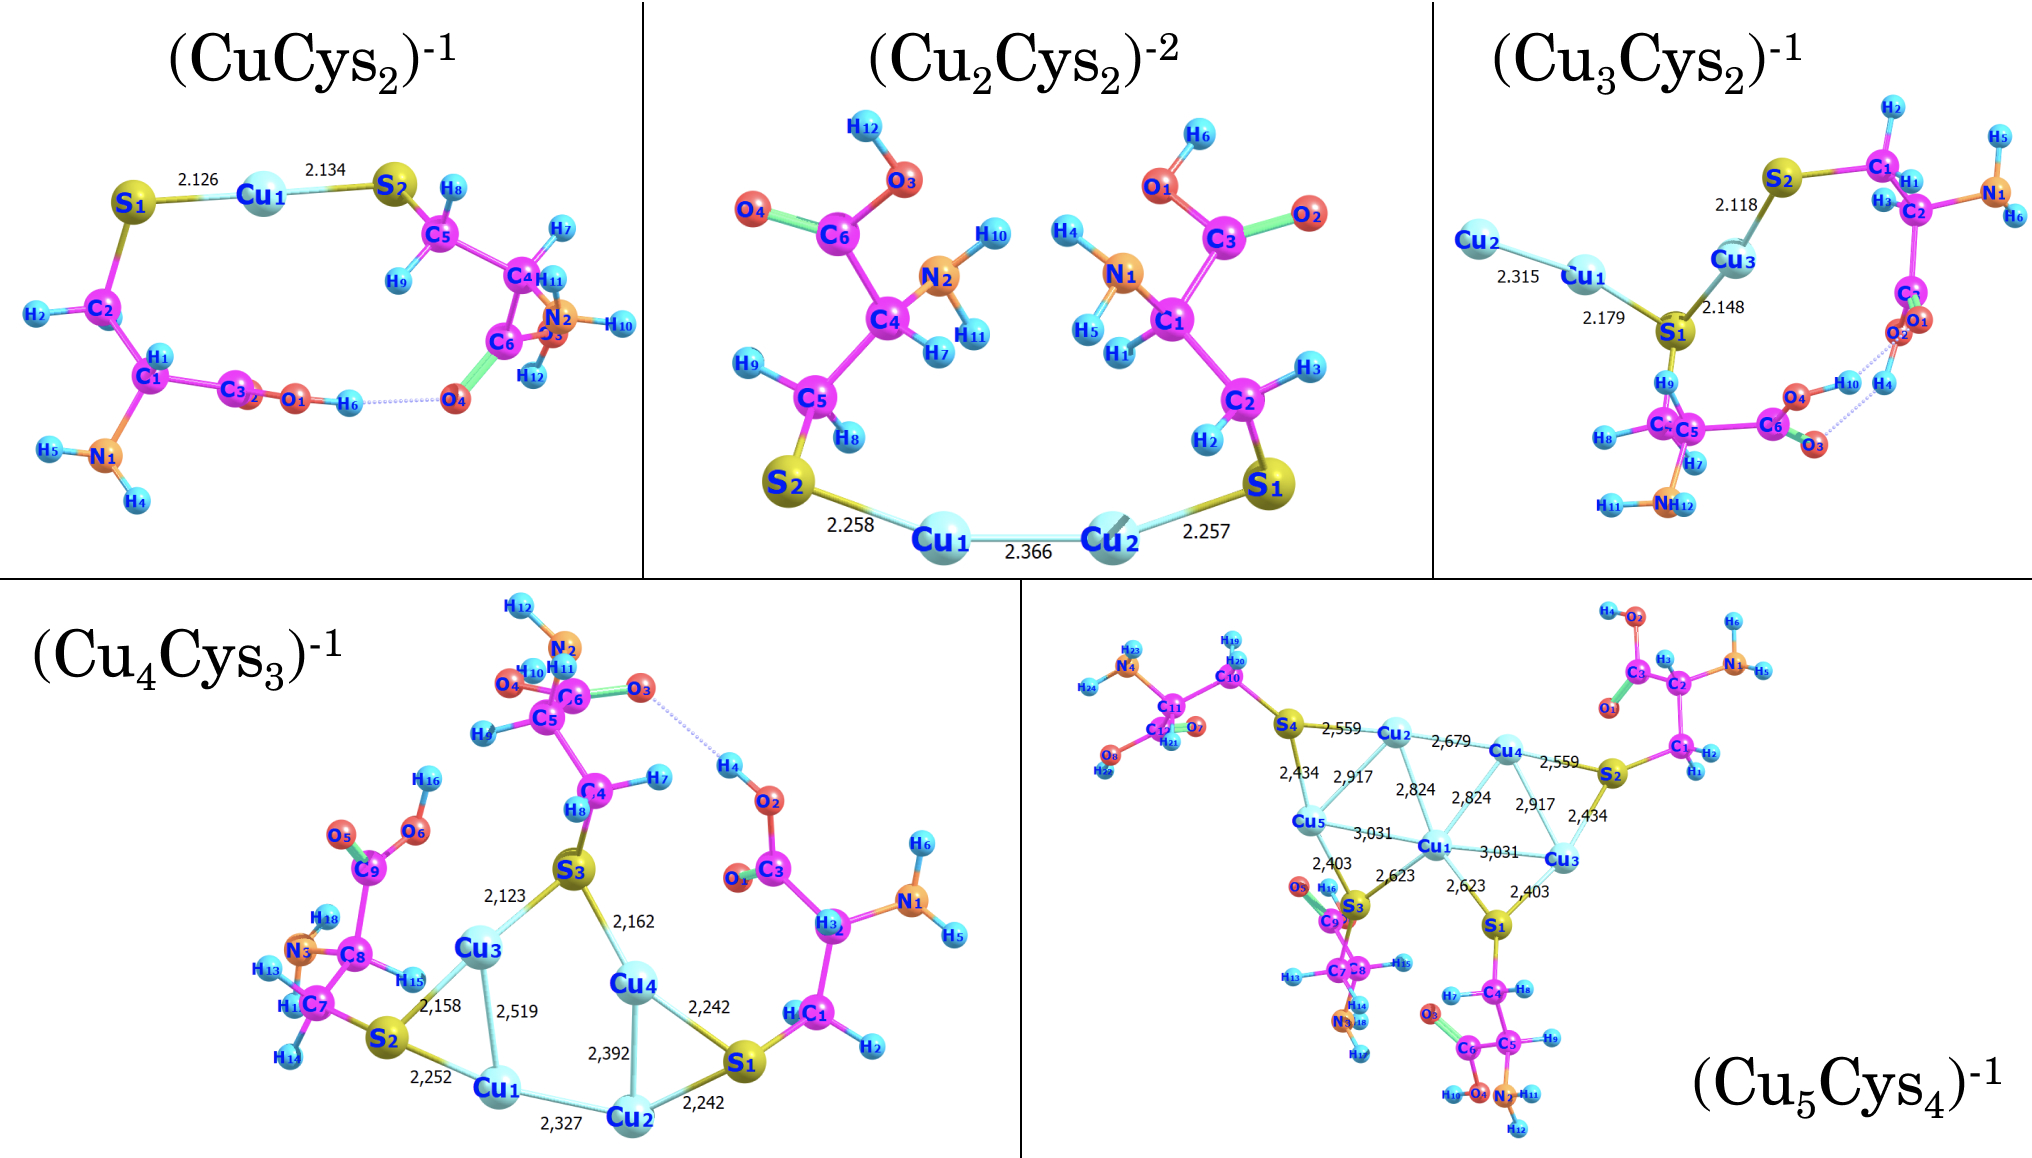
\includegraphics[width=\textwidth, frame]{pictures/opt_Cys_vac.jpg}
		\caption{Оптимизированные {в газовой фазе} геометрии комплексов, стабилизированных цистеином (метод: MP2 def2-TZVP).}
		\label{fig_geoopt_Cys_vac}
	\end{figure}
	
%	Структурные параметры комплексов, стабилизированных метилтиогруппой, отличаются сравнительно мало от параметров комплексов с цистеином в качестве лиганда. В случае с \ce{CuL2}, длины связей и валентные углы в газовой фазе и в воде практически идентичны, однако двугранные углы отличаются весьма значительно. Схожая ситуация наблюдается и для комплекса с двухатомным кластером, с несколькими отличиями.Первое заключается в виде сокращения \ce{Cu-Cu} связи на 0,03Å в газовой фазе (2,366Å вместо 2,394Å). Также, в газовой фазе валентные углы для связей \ce{Cu-S-C} уменьшились приблизительно на 10º, а для связей \ce{Cu-Cu-S} — на 20º. Та же закономерность наблюдается и для двугранных углов. В воде, при этом, полученные данные не так сильно разнятся друг с дургом.

	Структурные параметры комплексов, стабилизированных метилтиогруппой, в целом незначительно отличаются от соответствующих параметров комплексов, в которых в качестве лиганда выступает цистеин. Это указывает на то, что замена лиганда не приводит к радикальной перестройке координационной структуры, а оказывает лишь умеренное влияние на геометрию систем.
	
	Для комплекса \ce{CuL2} наблюдается практически полное совпадение длин связей и валентных углов как в газовой фазе, так и в водной среде. Однако двугранные углы в этих случаях различаются весьма существенно, что свидетельствует о различиях в пространственной ориентации лигандов при сохранении основных геометрических параметров.
	
	Сходная картина характерна и для комплекса с двухатомным кластером меди, хотя в этом случае можно выделить ряд дополнительных особенностей. Во-первых, в газовой фазе наблюдается небольшое сокращение связи \ce{Cu-Cu}: её длина уменьшается на 0,03Å (2,366Å по сравнению с 2,394Å). Во-вторых, валентные углы также демонстрируют систематическое уменьшение: для углов \ce{Cu-S-C} оно составляет порядка 10º, тогда как для углов \ce{Cu-Cu-S} — около 20º. Аналогичная тенденция прослеживается и для двугранных углов, что указывает на согласованное изменение пространственной конфигурации комплекса.
	
	В водной среде, напротив, различия между соответствующими параметрами оказываются значительно менее выраженными, что, вероятно, связано со стабилизирующим влиянием растворителя, сглаживающим геометрические отклонения между комплексами с различными лигандами.
	
	\begin{table}[H]
		\caption{Основные структурные параметры комплексов \ce{[CuCys2]^{-1}} и \ce{[Cu2Cys2]^{-2}}.}
		\label{tab4}
		\centering
		\begin{tabular}{ccccc|cccc|}
			\hline
			\multicolumn{4}{|c|}{\textbf{CuCys2}}                                                                                         & \textbf{} & \multicolumn{4}{c|}{\textbf{Cu2Cys2}}                                                                     \\ \hline
			\multicolumn{4}{|c|}{\textit{длины связей (Å)}}                                                                               & \textit{} & \multicolumn{4}{c|}{\textit{длины связей (Å)}}                                                            \\ \hline
			\multicolumn{1}{|c|}{атомы}        & \multicolumn{1}{c|}{вакуум} & \multicolumn{1}{c|}{вода}  & \multicolumn{1}{c|}{разность} &           & \multicolumn{1}{c|}{атомы}         & \multicolumn{1}{c|}{вакуум} & \multicolumn{1}{c|}{вода}   & разность \\ \hline
			\multicolumn{1}{|c|}{C2-S1}        & \multicolumn{1}{c|}{1,824}  & \multicolumn{1}{c|}{1,828} & \multicolumn{1}{c|}{-0,004}   &           & \multicolumn{1}{c|}{C2-S1}         & \multicolumn{1}{c|}{1,828}  & \multicolumn{1}{c|}{1,831}  & -0,003   \\ \cline{1-4} \cline{6-9} 
			\multicolumn{1}{|c|}{C5-S2}        & \multicolumn{1}{c|}{1,824}  & \multicolumn{1}{c|}{1,833} & \multicolumn{1}{c|}{-0,009}   &           & \multicolumn{1}{c|}{C5-S2}         & \multicolumn{1}{c|}{1,828}  & \multicolumn{1}{c|}{1,832}  & -0,004   \\ \cline{1-4} \cline{6-9} 
			\multicolumn{1}{|c|}{S2-Cu1}       & \multicolumn{1}{c|}{2,134}  & \multicolumn{1}{c|}{2,133} & \multicolumn{1}{c|}{0,001}    &           & \multicolumn{1}{c|}{S2-Cu1}        & \multicolumn{1}{c|}{2,258}  & \multicolumn{1}{c|}{2,178}  & 0,080    \\ \cline{1-4} \cline{6-9} 
			\multicolumn{1}{|c|}{S1-Cu1}       & \multicolumn{1}{c|}{2,126}  & \multicolumn{1}{c|}{2,136} & \multicolumn{1}{c|}{-0,010}   &           & \multicolumn{1}{c|}{S1-Cu2}        & \multicolumn{1}{c|}{2,257}  & \multicolumn{1}{c|}{2,190}  & 0,067    \\ \cline{1-4} \cline{6-9} 
			\multicolumn{4}{|c|}{\textit{валентные углы (º)}}                                                                             & \textit{} & \multicolumn{1}{c|}{Cu1-Cu2}       & \multicolumn{1}{c|}{2,366}  & \multicolumn{1}{c|}{2,350}  & 0,016    \\ \cline{1-4} \cline{6-9} 
			\multicolumn{1}{|c|}{атомы}        & \multicolumn{1}{c|}{вакуум} & \multicolumn{1}{c|}{вода}  & \multicolumn{1}{c|}{разность} &           & \multicolumn{4}{c|}{\textit{валентные углы (º)}}                                                          \\ \cline{1-4} \cline{6-9} 
			\multicolumn{1}{|c|}{C2-S1-Cu1}    & \multicolumn{1}{c|}{106,2}  & \multicolumn{1}{c|}{101,7} & \multicolumn{1}{c|}{4,4}      &           & \multicolumn{1}{c|}{атомы}         & \multicolumn{1}{c|}{вакуум} & \multicolumn{1}{c|}{вода}   & разность \\ \cline{1-4} \cline{6-9} 
			\multicolumn{1}{|c|}{C5-S2-Cu1}    & \multicolumn{1}{c|}{103,5}  & \multicolumn{1}{c|}{100,1} & \multicolumn{1}{c|}{3,5}      &           & \multicolumn{1}{c|}{C2-S1-Cu2}     & \multicolumn{1}{c|}{89,7}   & \multicolumn{1}{c|}{96,3}   & -6,6     \\ \cline{1-4} \cline{6-9} 
			\multicolumn{1}{|c|}{S1-Cu1-S2}    & \multicolumn{1}{c|}{178,2}  & \multicolumn{1}{c|}{174,9} & \multicolumn{1}{c|}{3,3}      &           & \multicolumn{1}{c|}{C5-S2-Cu1}     & \multicolumn{1}{c|}{89,5}   & \multicolumn{1}{c|}{105,9}  & -16,4    \\ \cline{1-4} \cline{6-9} 
			\multicolumn{4}{|c|}{\textit{дигедральные углы   (º)}}                                                                        & \textit{} & \multicolumn{1}{c|}{S1-Cu2-Cu1}    & \multicolumn{1}{c|}{158,0}  & \multicolumn{1}{c|}{174,5}  & -16,6    \\ \cline{1-4} \cline{6-9} 
			\multicolumn{1}{|c|}{атомы}        & \multicolumn{1}{c|}{вакуум} & \multicolumn{1}{c|}{вода}  & \multicolumn{1}{c|}{разность} &           & \multicolumn{1}{c|}{S2-Cu1-Cu2}    & \multicolumn{1}{c|}{157,9}  & \multicolumn{1}{c|}{177,9}  & -20,0    \\ \cline{1-4} \cline{6-9} 
			\multicolumn{1}{|c|}{C2-S1-Cu1-S2} & \multicolumn{1}{c|}{124,6}  & \multicolumn{1}{c|}{-54,8} & \multicolumn{1}{c|}{179,4}    &           & \multicolumn{4}{c|}{\textit{дигедральные углы (º)}}                                                       \\ \cline{1-4} \cline{6-9} 
			\multicolumn{1}{|c|}{C5-S2-Cu1-S1} & \multicolumn{1}{c|}{-43,4}  & \multicolumn{1}{c|}{16,3}  & \multicolumn{1}{c|}{-59,7}    &           & \multicolumn{1}{c|}{атомы}         & \multicolumn{1}{c|}{вакуум} & \multicolumn{1}{c|}{вода}   & разность \\ \cline{1-4} \cline{6-9} 
			&                             &                            &                               &           & \multicolumn{1}{c|}{C2-S1-Cu2-Cu1} & \multicolumn{1}{c|}{-17,6}  & \multicolumn{1}{c|}{4,8}    & -22,4    \\ \cline{6-9} 
			&                             &                            &                               &           & \multicolumn{1}{c|}{C5-S2-Cu1-Cu2} & \multicolumn{1}{c|}{-21,2}  & \multicolumn{1}{c|}{-178,1} & 156,9    \\ \cline{6-9} 
			&                             &                            &                               &           & \multicolumn{1}{c|}{S2-Cu1-Cu2-S1} & \multicolumn{1}{c|}{-53,5}  & \multicolumn{1}{c|}{124,4}  & -178,0   \\ \cline{6-9} 
		\end{tabular}
	\end{table}
	
%	Для структуры \ce{Cu3L2} изменения в геометрических параметрах комплексов незначительны. Длины валентных связей отличаются в пределах погрешности, а валентные углы стабильно меньше на 10º для комплексов, стабилизированных цистеином. Двугранные углы снова сильно расходятся для комплексов с двумя лигандами. Значения длин валентных связей, полученные для комплекса с четырёхатомным кластером меди, тоже слабо отличаются для двух лигандов. 

	Для структуры \ce{Cu3L2} изменения геометрических параметров при замене лиганда носят, в целом, незначительный характер. Длины валентных связей для соответствующих комплексов отличаются лишь в пределах вычислительной погрешности, что свидетельствует о сохранении общей конфигурации координационного окружения. При этом валентные углы для комплексов, стабилизированных цистеином, оказываются систематически меньшими примерно на 10º, что может указывать на небольшое уплотнение структуры.

	В то же время двугранные углы демонстрируют существенно большее расхождение, особенно для комплексов с двумя лигандами, что отражает более гибкий характер пространственной ориентации лигандов и возможные конформационные различия между структурами.

	Аналогичная тенденция наблюдается и для комплекса с четырёхатомным кластером меди: значения длин валентных связей для систем с различными лигандами различаются незначительно, что дополнительно подтверждает вывод о слабом влиянии замены лиганда на основные геометрические параметры в данных структурах.
	
%	В случае с комплексом \ce{Cu5L4} мы можем анализировать только значения полученные в газовой фазе: в воде не были получены адекватные результаты. Связи \ce{C-S} удлинились на 0,01Å, \ce{Cu-S} — от 0,2Å до 0,4Å, как и длины связей \ce{Cu-Cu}.
	
	В случае комплекса \ce{Cu5L4} анализ ограничивается данными, полученными для газовой фазы, поскольку расчёты в водной среде не позволили получить корректные и воспроизводимые результаты. Это накладывает определённые ограничения на интерпретацию, однако имеющиеся данные всё же позволяют выявить характерные тенденции в изменении геометрии.
	
	\begin{table}[H]
		\caption{Основные структурные параметры комплексов \ce{[Cu3Cys2]^{-1}} и \ce{[Cu5Cys4]^{-1}}.}
		\label{tab5}
		\centering
		\begin{tabular}{|cccc|ccc}
			\cline{1-4} \cline{6-7}
			\multicolumn{4}{|c|}{\textbf{Cu3Cys2}}                                                                      & \multicolumn{1}{c|}{} & \multicolumn{2}{c|}{\multirow{2}{*}{\textbf{Cu5Cys4}}}                        \\ \cline{1-4}
			\multicolumn{4}{|c|}{\textit{длины связей (Å)}}                                                             & \multicolumn{1}{c|}{} & \multicolumn{2}{c|}{}                                                         \\ \cline{1-4} \cline{6-7} 
			\multicolumn{1}{|c|}{атомы}          & \multicolumn{1}{c|}{вакуум} & \multicolumn{1}{c|}{вода}   & разность & \multicolumn{1}{c|}{} & \multicolumn{1}{c|}{атомы}   & \multicolumn{1}{c|}{\textit{длины связей в вакууме (Å)}} \\ \cline{1-4} \cline{6-7} 
			\multicolumn{1}{|c|}{C1-S2}          & \multicolumn{1}{c|}{1,826}  & \multicolumn{1}{c|}{1,826}  & 0,000    & \multicolumn{1}{c|}{} & \multicolumn{1}{c|}{C4-S1}   & \multicolumn{1}{c|}{1,820}                     \\ \cline{1-4} \cline{6-7} 
			\multicolumn{1}{|c|}{C4-S1}          & \multicolumn{1}{c|}{1,836}  & \multicolumn{1}{c|}{2,835}  & -0,999   & \multicolumn{1}{c|}{} & \multicolumn{1}{c|}{C1-S2}   & \multicolumn{1}{c|}{1,820}                     \\ \cline{1-4} \cline{6-7} 
			\multicolumn{1}{|c|}{S2-Cu3}         & \multicolumn{1}{c|}{2,118}  & \multicolumn{1}{c|}{2,137}  & -0,019   & \multicolumn{1}{c|}{} & \multicolumn{1}{c|}{C7-S3}   & \multicolumn{1}{c|}{1,820}                     \\ \cline{1-4} \cline{6-7} 
			\multicolumn{1}{|c|}{S1-Cu3}         & \multicolumn{1}{c|}{2,148}  & \multicolumn{1}{c|}{2,163}  & -0,015   & \multicolumn{1}{c|}{} & \multicolumn{1}{c|}{C10-S4}  & \multicolumn{1}{c|}{1,820}                     \\ \cline{1-4} \cline{6-7} 
			\multicolumn{1}{|c|}{S1-Cu1}         & \multicolumn{1}{c|}{2,179}  & \multicolumn{1}{c|}{2,177}  & 0,002    & \multicolumn{1}{c|}{} & \multicolumn{1}{c|}{S1-Cu3}  & \multicolumn{1}{c|}{2,403}                     \\ \cline{1-4} \cline{6-7} 
			\multicolumn{1}{|c|}{Cu1-Cu2}        & \multicolumn{1}{c|}{2,315}  & \multicolumn{1}{c|}{2,308}  & 0,007    & \multicolumn{1}{c|}{} & \multicolumn{1}{c|}{S1-Cu1}  & \multicolumn{1}{c|}{2,623}                     \\ \cline{1-4} \cline{6-7} 
			\multicolumn{4}{|c|}{\textit{валентные углы (º)}}                                                           & \multicolumn{1}{c|}{} & \multicolumn{1}{c|}{S2-Cu3}  & \multicolumn{1}{c|}{2,434}                     \\ \cline{1-4} \cline{6-7} 
			\multicolumn{1}{|c|}{атомы}          & \multicolumn{1}{c|}{вакуум} & \multicolumn{1}{c|}{вода}   & разность & \multicolumn{1}{c|}{} & \multicolumn{1}{c|}{S2-Cu4}  & \multicolumn{1}{c|}{2,559}                     \\ \cline{1-4} \cline{6-7} 
			\multicolumn{1}{|c|}{C1-S2-Cu3}      & \multicolumn{1}{c|}{113,1}  & \multicolumn{1}{c|}{107,0}  & 6,1      & \multicolumn{1}{c|}{} & \multicolumn{1}{c|}{S3-Cu1}  & \multicolumn{1}{c|}{2,623}                     \\ \cline{1-4} \cline{6-7} 
			\multicolumn{1}{|c|}{C4-S1-Cu3}      & \multicolumn{1}{c|}{111,4}  & \multicolumn{1}{c|}{99,7}   & 11,7     & \multicolumn{1}{c|}{} & \multicolumn{1}{c|}{S3-Cu5}  & \multicolumn{1}{c|}{2,403}                     \\ \cline{1-4} \cline{6-7} 
			\multicolumn{1}{|c|}{C4-S1-Cu1}      & \multicolumn{1}{c|}{98,1}   & \multicolumn{1}{c|}{106,3}  & -8,2     & \multicolumn{1}{c|}{} & \multicolumn{1}{c|}{S4-Cu5}  & \multicolumn{1}{c|}{2,434}                     \\ \cline{1-4} \cline{6-7} 
			\multicolumn{1}{|c|}{S2-Cu3-S1}      & \multicolumn{1}{c|}{172,4}  & \multicolumn{1}{c|}{170,2}  & 2,3      & \multicolumn{1}{c|}{} & \multicolumn{1}{c|}{S4-Cu2}  & \multicolumn{1}{c|}{2,559}                     \\ \cline{1-4} \cline{6-7} 
			\multicolumn{1}{|c|}{Cu3-S1-Cu1}     & \multicolumn{1}{c|}{78,4}   & \multicolumn{1}{c|}{78,8}   & -0,4     & \multicolumn{1}{c|}{} & \multicolumn{1}{c|}{Cu1-Cu3} & \multicolumn{1}{c|}{3,031}                     \\ \cline{1-4} \cline{6-7} 
			\multicolumn{1}{|c|}{S1-Cu1-Cu2}     & \multicolumn{1}{c|}{168,1}  & \multicolumn{1}{c|}{170,9}  & -2,8     & \multicolumn{1}{c|}{} & \multicolumn{1}{c|}{Cu1-Cu4} & \multicolumn{1}{c|}{2,824}                     \\ \cline{1-4} \cline{6-7} 
			\multicolumn{4}{|c|}{\textit{дигедральные углы   (º)}}                                                      & \multicolumn{1}{c|}{} & \multicolumn{1}{c|}{Cu1-Cu2} & \multicolumn{1}{c|}{2,824}                     \\ \cline{1-4} \cline{6-7} 
			\multicolumn{1}{|c|}{атомы}          & \multicolumn{1}{c|}{вакуум} & \multicolumn{1}{c|}{вода}   & разность & \multicolumn{1}{c|}{} & \multicolumn{1}{c|}{Cu1-Cu5} & \multicolumn{1}{c|}{3,031}                     \\ \cline{1-4} \cline{6-7} 
			\multicolumn{1}{|c|}{C1-S2-Cu3-S1}   & \multicolumn{1}{c|}{148,5}  & \multicolumn{1}{c|}{-127,5} & 276,0    & \multicolumn{1}{c|}{} & \multicolumn{1}{c|}{Cu3-Cu4} & \multicolumn{1}{c|}{2,917}                     \\ \cline{1-4} \cline{6-7} 
			\multicolumn{1}{|c|}{S2-Cu3-S1-C4}   & \multicolumn{1}{c|}{117,1}  & \multicolumn{1}{c|}{-168,1} & 285,2    & \multicolumn{1}{c|}{} & \multicolumn{1}{c|}{Cu4-Cu2} & \multicolumn{1}{c|}{2,679}                     \\ \cline{1-4} \cline{6-7} 
			\multicolumn{1}{|c|}{S2-Cu3-S1-Cu1}  & \multicolumn{1}{c|}{22,8}   & \multicolumn{1}{c|}{-168,1} & 190,9    & \multicolumn{1}{c|}{} & \multicolumn{1}{c|}{Cu2-Cu5} & \multicolumn{1}{c|}{2,917}                     \\ \cline{1-4} \cline{6-7} 
			\multicolumn{1}{|c|}{Cu3-S1-Cu1-Cu2} & \multicolumn{1}{c|}{133,7}  & \multicolumn{1}{c|}{-167,8} & 301,4    &                       &                              &                                                \\ \cline{1-4}
			\multicolumn{1}{|c|}{C4-S1-Cu1-Cu2}  & \multicolumn{1}{c|}{23,4}   & \multicolumn{1}{c|}{-70,8}  & 94,2     &                       &                              & \textit{}                                      \\ \cline{1-4}
		\end{tabular}
	\end{table}

	
	\begin{table}[H]
		\caption{Основные структурные параметры комплексов \ce{[Cu4Cys3]^{-1}}.}
		\label{tab6}
		\centering
		\begin{tabular}{|cccc|}
			\hline
			\multicolumn{4}{|c|}{\textbf{Cu4Cys3}}                                                              \\ \hline
			\multicolumn{4}{|c|}{\textit{длины связей (Å)}}                                                     \\ \hline
			\multicolumn{1}{|c|}{атомы}   & \multicolumn{1}{c|}{вакуум} & \multicolumn{1}{c|}{вода}  & разность \\ \hline
			\multicolumn{1}{|c|}{C1-S1}   & \multicolumn{1}{c|}{1,830}  & \multicolumn{1}{c|}{1,832} & -0,002   \\ \hline
			\multicolumn{1}{|c|}{C7-S2}   & \multicolumn{1}{c|}{1,832}  & \multicolumn{1}{c|}{1,831} & 0,001    \\ \hline
			\multicolumn{1}{|c|}{C4-S3}   & \multicolumn{1}{c|}{1,823}  & \multicolumn{1}{c|}{1,831} & -0,008   \\ \hline
			\multicolumn{1}{|c|}{S1-Cu4}  & \multicolumn{1}{c|}{2,242}  & \multicolumn{1}{c|}{2,212} & 0,030    \\ \hline
			\multicolumn{1}{|c|}{S1-Cu2}  & \multicolumn{1}{c|}{2,242}  & \multicolumn{1}{c|}{2,240} & 0,002    \\ \hline
			\multicolumn{1}{|c|}{S2-Cu1}  & \multicolumn{1}{c|}{2,252}  & \multicolumn{1}{c|}{2,208} & 0,044    \\ \hline
			\multicolumn{1}{|c|}{S2-Cu3}  & \multicolumn{1}{c|}{2,158}  & \multicolumn{1}{c|}{2,231} & -0,073   \\ \hline
			\multicolumn{1}{|c|}{S3-Cu4}  & \multicolumn{1}{c|}{2,162}  & \multicolumn{1}{c|}{2,174} & -0,012   \\ \hline
			\multicolumn{1}{|c|}{S3-Cu3}  & \multicolumn{1}{c|}{2,123}  & \multicolumn{1}{c|}{2,195} & -0,072   \\ \hline
			\multicolumn{1}{|c|}{Cu1-Cu2} & \multicolumn{1}{c|}{2,327}  & \multicolumn{1}{c|}{2,319} & 0,008    \\ \hline
			\multicolumn{1}{|c|}{Cu3-Cu1} & \multicolumn{1}{c|}{2,519}  & \multicolumn{1}{c|}{2,484} & 0,035    \\ \hline
			\multicolumn{1}{|c|}{Cu2-Cu4} & \multicolumn{1}{c|}{2,392}  & \multicolumn{1}{c|}{2,488} & -0,096   \\ \hline
		\end{tabular}
	\end{table}
	
	Так, длины связей \ce{C-S} демонстрируют незначительное увеличение — примерно на 0,01Å, что указывает на минимальное влияние замены лиганда на данный тип взаимодействий. В то же время изменения для связей \ce{Cu-S} оказываются значительно более выраженными: их удлинение составляет от 0,2Å до 0,4Å. Сопоставимое увеличение наблюдается и для межатомных расстояний \ce{Cu-Cu}, что свидетельствует о заметной перестройке металлического каркаса комплекса под влиянием замены лиганда.
	
%	Обобщая написанное выше, геометрии комплексов, при замене лиганда в лице метилтиогруппы цистеином, несомненно изменились. В зависимости от конкретного комплекса, эти изменения разнятся от незначительных до существенных. Стоит отметить, что длины валентных связей отличаются не более, чем на 0,4Å, а валентные углы — не более, чем на 20º. Эти случаи являются исключениями из общей статистики, в среднем связи изменились не более, чем на 0,1Å при замене лиганда на цистеин, а углы — менее, чем на 10º. Проведённый далее анализ спектров поглощения комплексов \ce{Cu_n Cys_m} даст предстваление о влиянии этих изменений на модельные спектры поглощения.
	
	Обобщая изложенные выше результаты, можно заключить, что замена лиганда — метилтиогруппы на цистеиновый фрагмент — действительно приводит к изменениям геометрии комплексов. Однако степень этих изменений существенно зависит от конкретной структуры: в одних случаях они оказываются минимальными, тогда как в других становятся более выраженными и заметными.
	
	Следует подчеркнуть, что даже в наиболее отклоняющихся случаях изменения геометрических параметров остаются ограниченными: длины валентных связей отличаются не более чем на 0,4Å, а валентные углы — не более чем на 20º. При этом подобные значения можно рассматривать скорее как исключения из общей тенденции. В среднем же замена лиганда на цистеин приводит к значительно меньшим изменениям: длины связей варьируются не более чем на 0,1Å, а изменения валентных углов, как правило, не превышают 10º.
	
	Дальнейший анализ спектров поглощения комплексов \ce{Cu_n Cys_m} позволяет более детально оценить, каким образом указанные геометрические изменения отражаются на их электронных свойствах и, в частности, на характеристиках модельных спектров поглощения.
	
	
	\subsubsection*{Спектры поглощения комплексов}
	% \addcontentsline{toc}{subsubsection}{Спектры поглощения комплексов}
	
%	При помощи оптимальных DFT методов, которые были определены на примере структур \ce{Cu_n (SCH3)_m}, были построены модельные спектры поглощения комплексов. Полученные результаты представлены на Рис.\ths\ref{fig_abs_M06-2X_vac_cys} и Рис.\ths\ref{fig_abs_CAM-B3LYP_vac_cys} для функционалов M06-2X и CAM-B3LYP соответственно.

	С использованием оптимальных DFT-методов, выбранных на основании предварительного анализа структур \ce{Cu_n (SCH3)_m}, были рассчитаны модельные спектры поглощения исследуемых комплексов. Такой подход позволил обеспечить согласованность методологии и сопоставимость результатов для различных типов лигандов.
	
	Полученные спектры поглощения представлены на Рис.\ths\ref{fig_abs_M06-2X_vac_cys} и Рис.\ths\ref{fig_abs_CAM-B3LYP_vac_cys} для функционалов M06-2X и CAM-B3LYP соответственно. Сравнение этих данных позволяет оценить влияние выбора функционала на описание электронных переходов, а также выявить общие закономерности в спектральных характеристиках комплексов, стабилизированных цистеином.
	
%	Рассматривая спектры как таковые, можно предположить, что в растворе присутствовали двухатомный, трёхатомный и пятиатомный кластеры, опираясь на рассчёты, полученные методом M06-2X. При этом мы предпологаем, что расчётный спектр отличается от эксперименального не более, чем на 20нм. В этом предположении наиболее вероятным комплексом в растворе является \ce{Cu5Cys4}. Результаты для CAM-B3LYP отражают схожую карину: вероятно, в растворе присутствовало наибольшее количество \ce{Cu5Cys4}. Обобщая сказанное, в этом случае ни один из методов не даёт хорошего согласования с экспериментальным спектром поглощения. Однако, при должном предположении о допустимом смещении спектров, пятиатомный комплекс даёт наиболее приемлемое совпадение с экспериментом.
	
	Рассматривая полученные спектры в совокупности, можно предположить, что в растворе одновременно присутствуют кластеры меди различной размерности, а именно двух-, трёх- и пятиатомные структуры. Данное предположение основано на результатах расчётов, выполненных с использованием функционала M06-2X, которые демонстрируют наилучшее качественное соответствие экспериментальным данным для указанных систем. При этом принимается допущение, что различие между расчётными и экспериментальными спектрами не превышает 20 нм, что является разумной оценкой погрешности для применяемых методов квантово-химического моделирования.
	
	\begin{figure}[H]
		\centering
		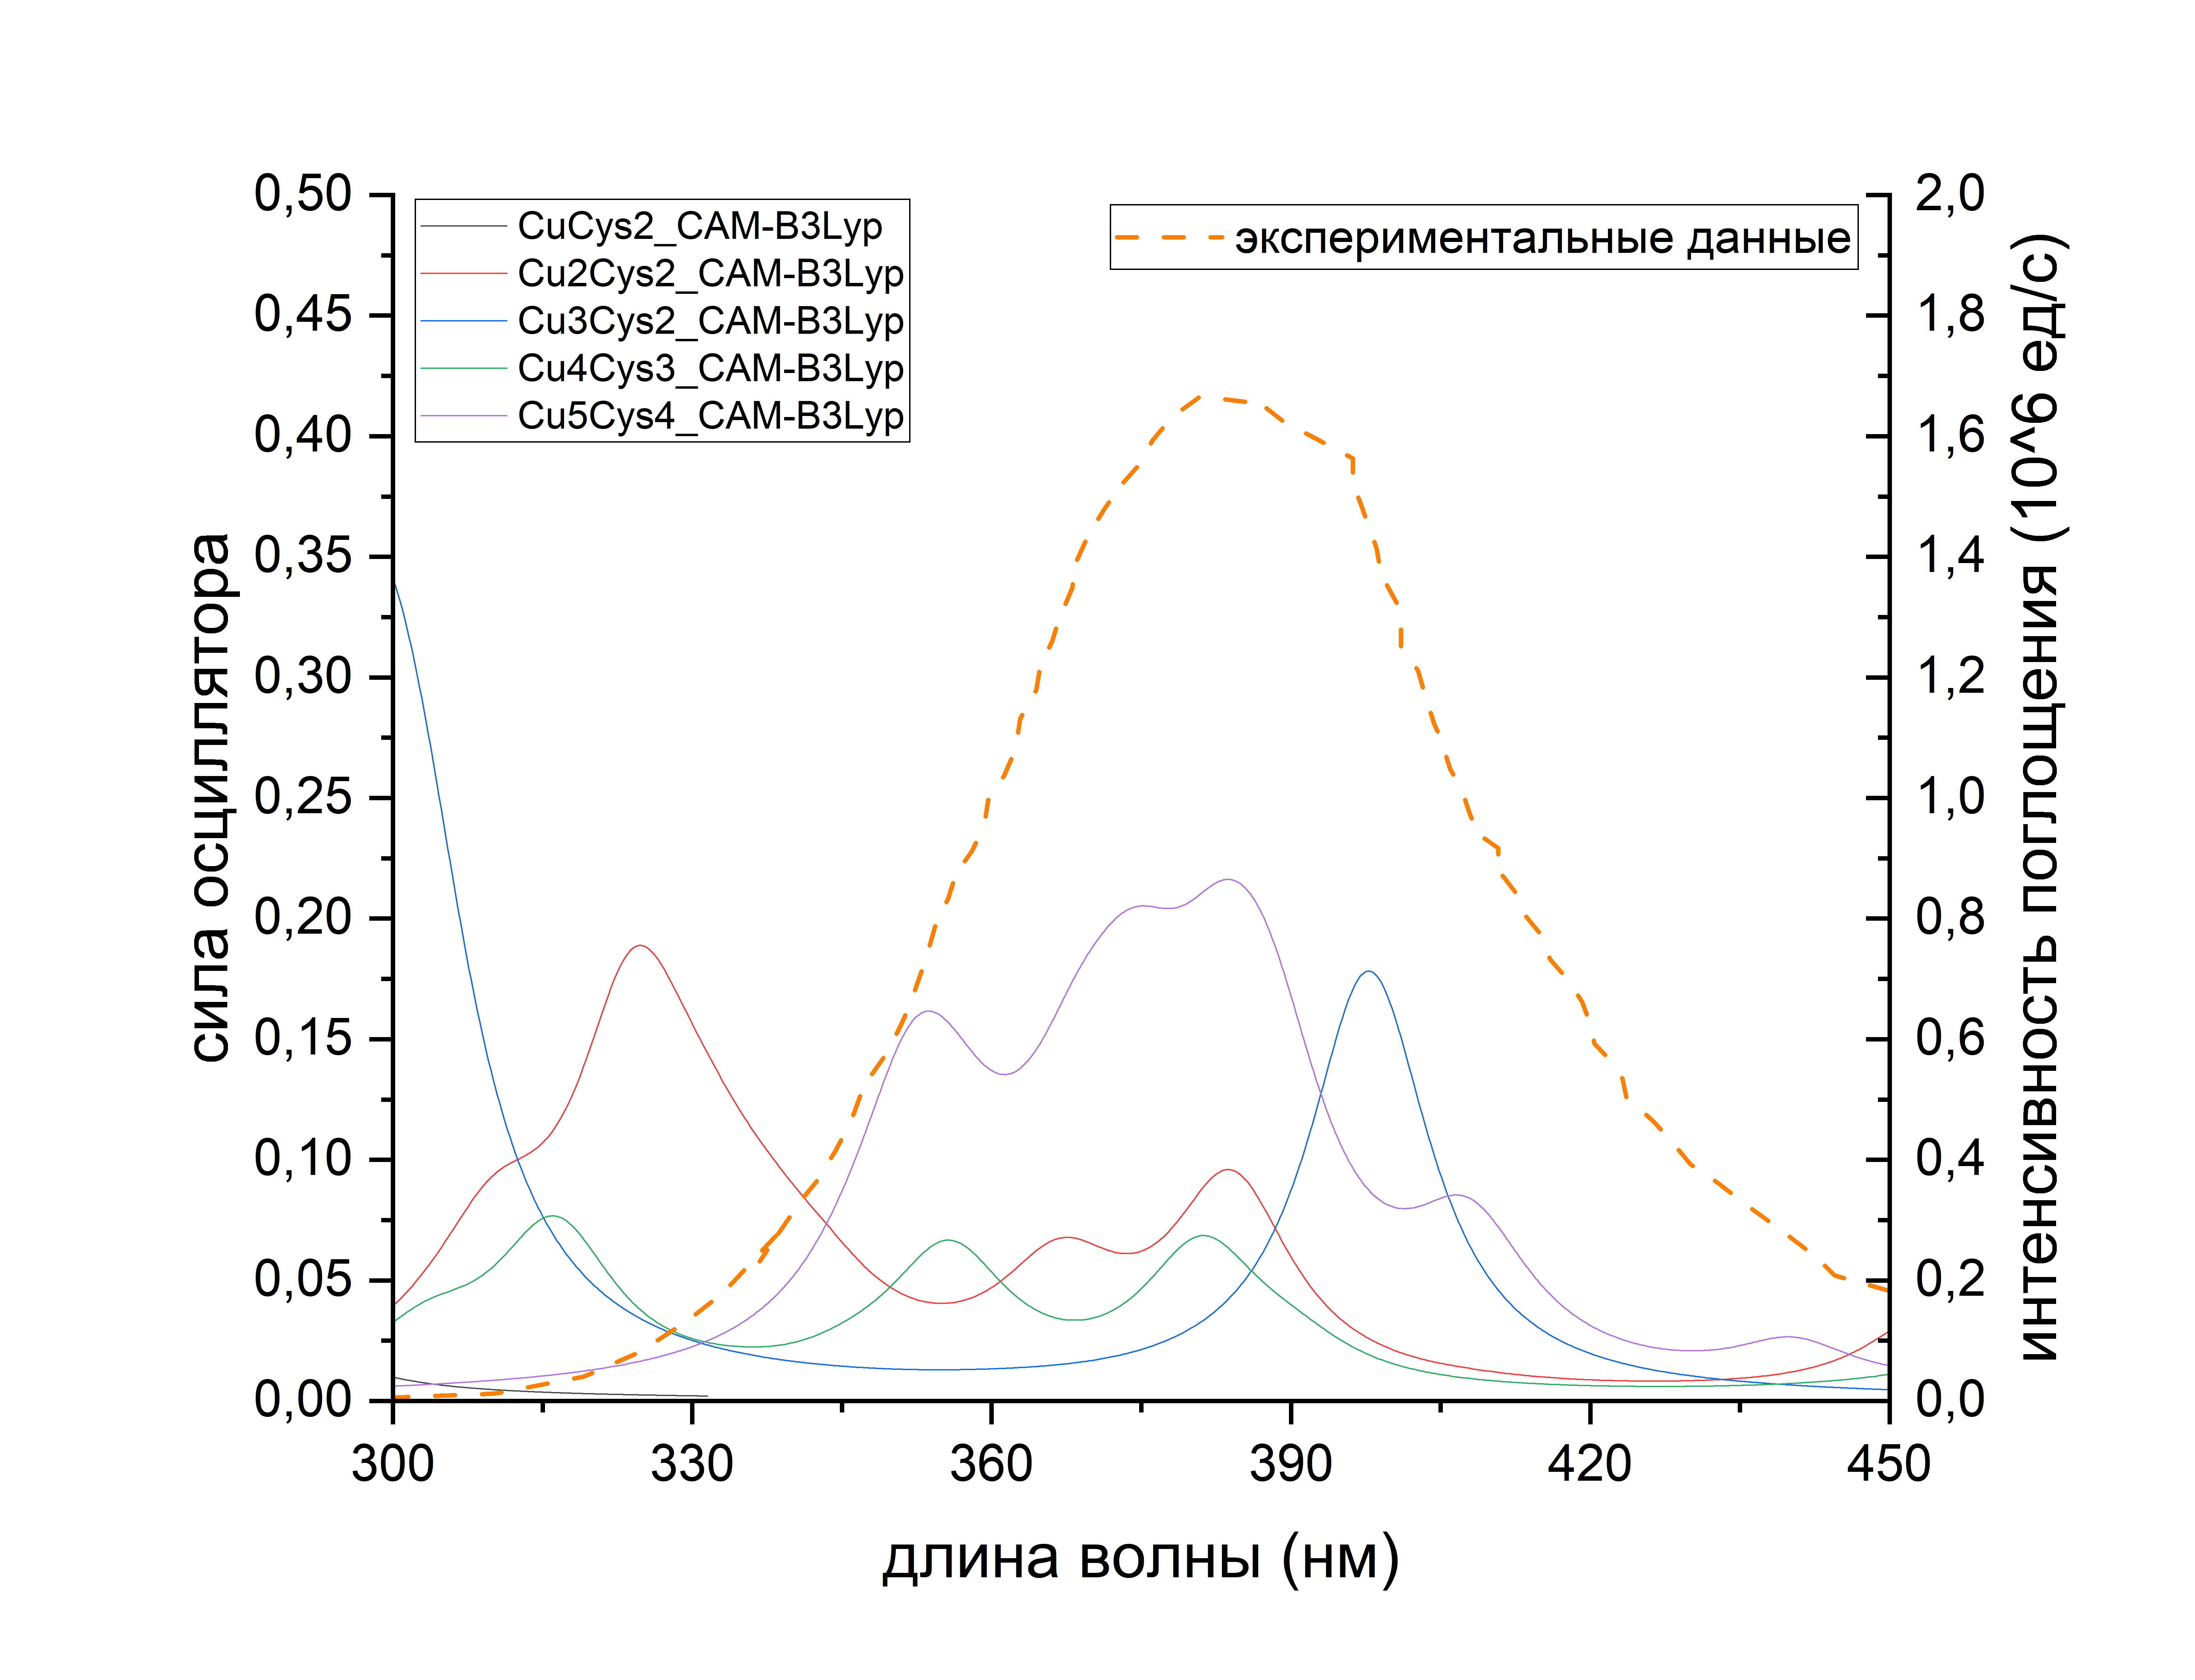
\includegraphics[width=0.7\textwidth]{pictures/spectra/Cys_CAM-B3Lyp_vacuum.png}
		\caption{Модельные спектры поглощения комплексов с цистеином, полученные при помощи функционала CAM-B3LYP в газовой фазе. Использовано Лоренцево уширение с полушириной 15нм.}
		\label{fig_abs_CAM-B3LYP_vac_cys}
	\end{figure}

	\begin{figure}[H]
		\centering
		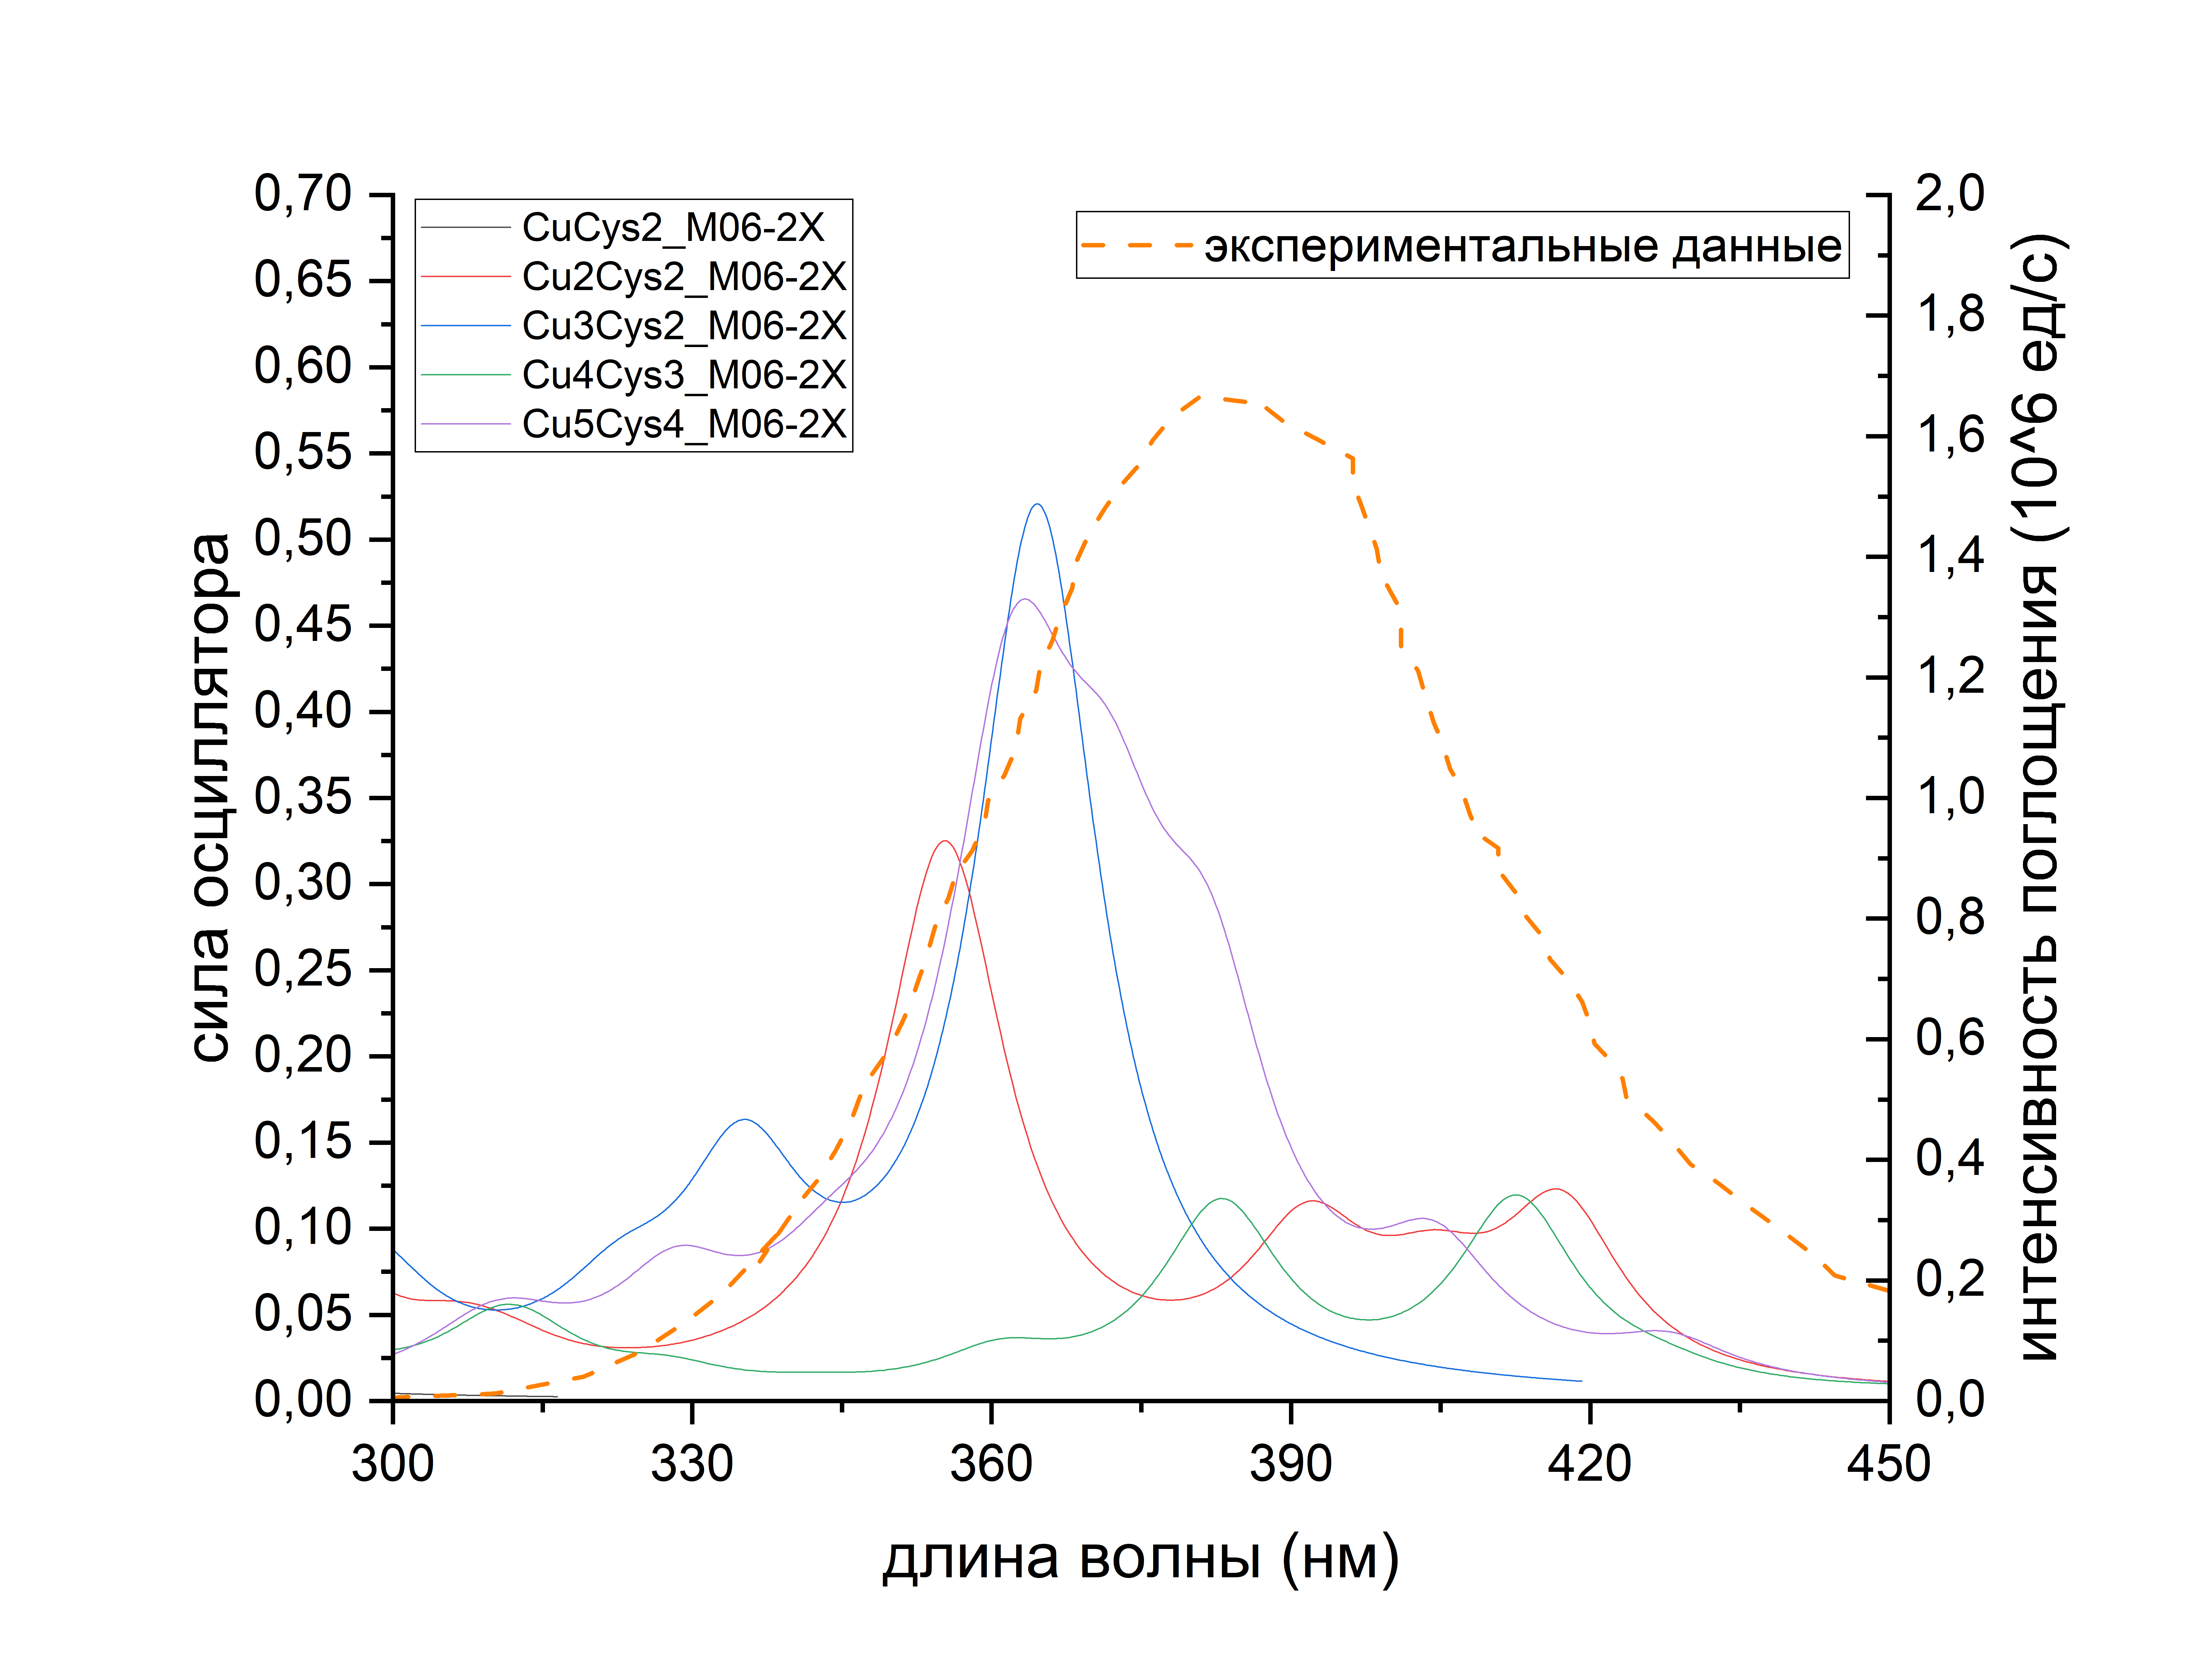
\includegraphics[width=0.7\textwidth]{pictures/spectra/Cys_M06-2X_vacuum.png } 
		\caption{Модельные спектры поглощения комплексов с цистеином, полученные при помощи функционала M06-2X в газовой фазе.  Использовано Лоренцево уширение с полушириной 15нм.}
		\label{fig_abs_M06-2X_vac_cys}
	\end{figure}

	В рамках такого предположения наиболее вероятным кандидатом на преобладающий в растворе комплекс оказывается структура \ce{Cu5Cys4}, поскольку именно для неё наблюдается наилучшее совпадение положения и формы спектральных максимумов с экспериментальным спектром поглощения. Аналогичный вывод можно сделать и на основании результатов, полученных с использованием метода CAM-B3LYP: несмотря на количественные отличия, общая картина остаётся схожей и также указывает на доминирующую роль комплекса \ce{Cu5Cys4} в растворе.
	
	Обобщая приведённые результаты, следует отметить, что ни один из использованных методов не обеспечивает полного количественного согласования с экспериментальным спектром поглощения. Тем не менее, при введении допустимого диапазона смещения спектров, пятиатомный комплекс демонстрирует наилучшее соответствие экспериментальным данным и, следовательно, может рассматриваться как наиболее вероятная форма существования системы в растворе.
	
	
%	Замена метилтиогруппы на цистеин изменила спектры. Меньше всего это повлияло на комплекс с трёхатомным кластером меди, что явно можно видеть на Рис.\ths\ref{fig_vac_COMP}. Как обсуждалось ранее, геометрические параметры этих комплексов практически не отличаются друг от друга для двух лигандов. Схожая ситуация наблюдается для структуры с ионом меди. Изменения в спектре претерпела и струкутра \ce{Cu2L2}. Для спектров, рассчитанных с помощью функционала M06-2X, наблюдается смещение основных переходов на 10 и 5 нм для правого и левого максимума соответственно (см.\ths Рис.\ths\ref{fig_vac_COMP}\ths(b), зелёная и красная кривые). Интенсивность второго пика, при этом, сильно понизилась, а переходы, составляющие его, стали различимы. Схожая зависимость наблюдается и для метода CAM-B3LYP, однако с меньшим смещением (не более, чем на 5 нм). Смещение наблюдается также для комплексов \ce{Cu4L3}, со смещением на 30нм и 40нм для крайних длинноволновых переходов, при расчёте методом M06-2X, и аналогичным смещением в 30нм и 25нм, для рассчитанных методом CAM-B3LYP спектров поглощения. Для этих комплексов наблюдалось небольшое удлинение связей. Наконец, для пятиатомного кластера наблюдается самое значительное изменение спектров, основные переходы увеличились по амплитуде для обоих методов, сместившись при этом приблизительно на 50нм в коротковолновую область. Это могло произойти вследствие значительного удлинения связей Cu-Cu и Cu-S. 

	Замена метилтиогруппы на цистеиновый фрагмент приводит к заметным изменениям в спектральных характеристиках исследуемых комплексов. При этом степень влияния данной замены существенно зависит от строения кластера. Наименьшее воздействие наблюдается для комплекса с трёхатомным кластером меди, что наглядно демонстрируется на Рис.\ths\ref{fig_vac_COMP}. Как уже обсуждалось ранее, геометрические параметры таких комплексов для двух различных лигандов практически совпадают, что, по-видимому, и обуславливает минимальные различия в их спектрах. Аналогичная ситуация имеет место и для структуры, содержащей одиночный ион меди, где изменения также оказываются незначительными.
	
	В то же время структура \ce{Cu2L2} демонстрирует более выраженные спектральные изменения. Для спектров, рассчитанных с использованием функционала M06-2X, наблюдается смещение основных электронных переходов: примерно на 10 нм для правого максимума и на 5 нм для левого (см.\ths Рис.\ths\ref{fig_vac_COMP}\ths(b), зелёная и красная кривые). Помимо этого, интенсивность второго пика существенно снижается, а составляющие его переходы становятся более отчётливо различимыми, что указывает на перераспределение вкладов отдельных возбуждённых состояний. Сходная тенденция прослеживается и при использовании метода CAM-B3LYP, однако величина смещения в этом случае оказывается меньше и не превышает 5 нм.
	
	Для комплексов \ce{Cu4L3} также фиксируется заметное смещение спектральных максимумов. В частности, при расчётах методом M06-2X длинноволновые переходы смещаются на 30 нм и 40 нм, тогда как для спектров, полученных с применением CAM-B3LYP, соответствующие смещения составляют 30 нм и 25 нм. Следует отметить, что для данных комплексов было зафиксировано некоторое удлинение межатомных связей, что, вероятно, связано с наблюдаемыми изменениями спектров.
	
	Наконец, наиболее существенные изменения обнаруживаются для пятиатомного кластера меди. В этом случае основные переходы характеризуются увеличением интенсивности для обоих использованных методов расчёта, а также смещением примерно на 50 нм в коротковолновую область. Вероятной причиной таких значительных изменений может являться заметное удлинение связей Cu–Cu и Cu–S, приводящее к перераспределению электронной плотности и, как следствие, к изменению энергетической структуры возбуждённых состояний.


	\begin{figure}[H]
		\centering
		
		\subfloat[Комплекс \ce{[CuL2]^{-1}}]{ 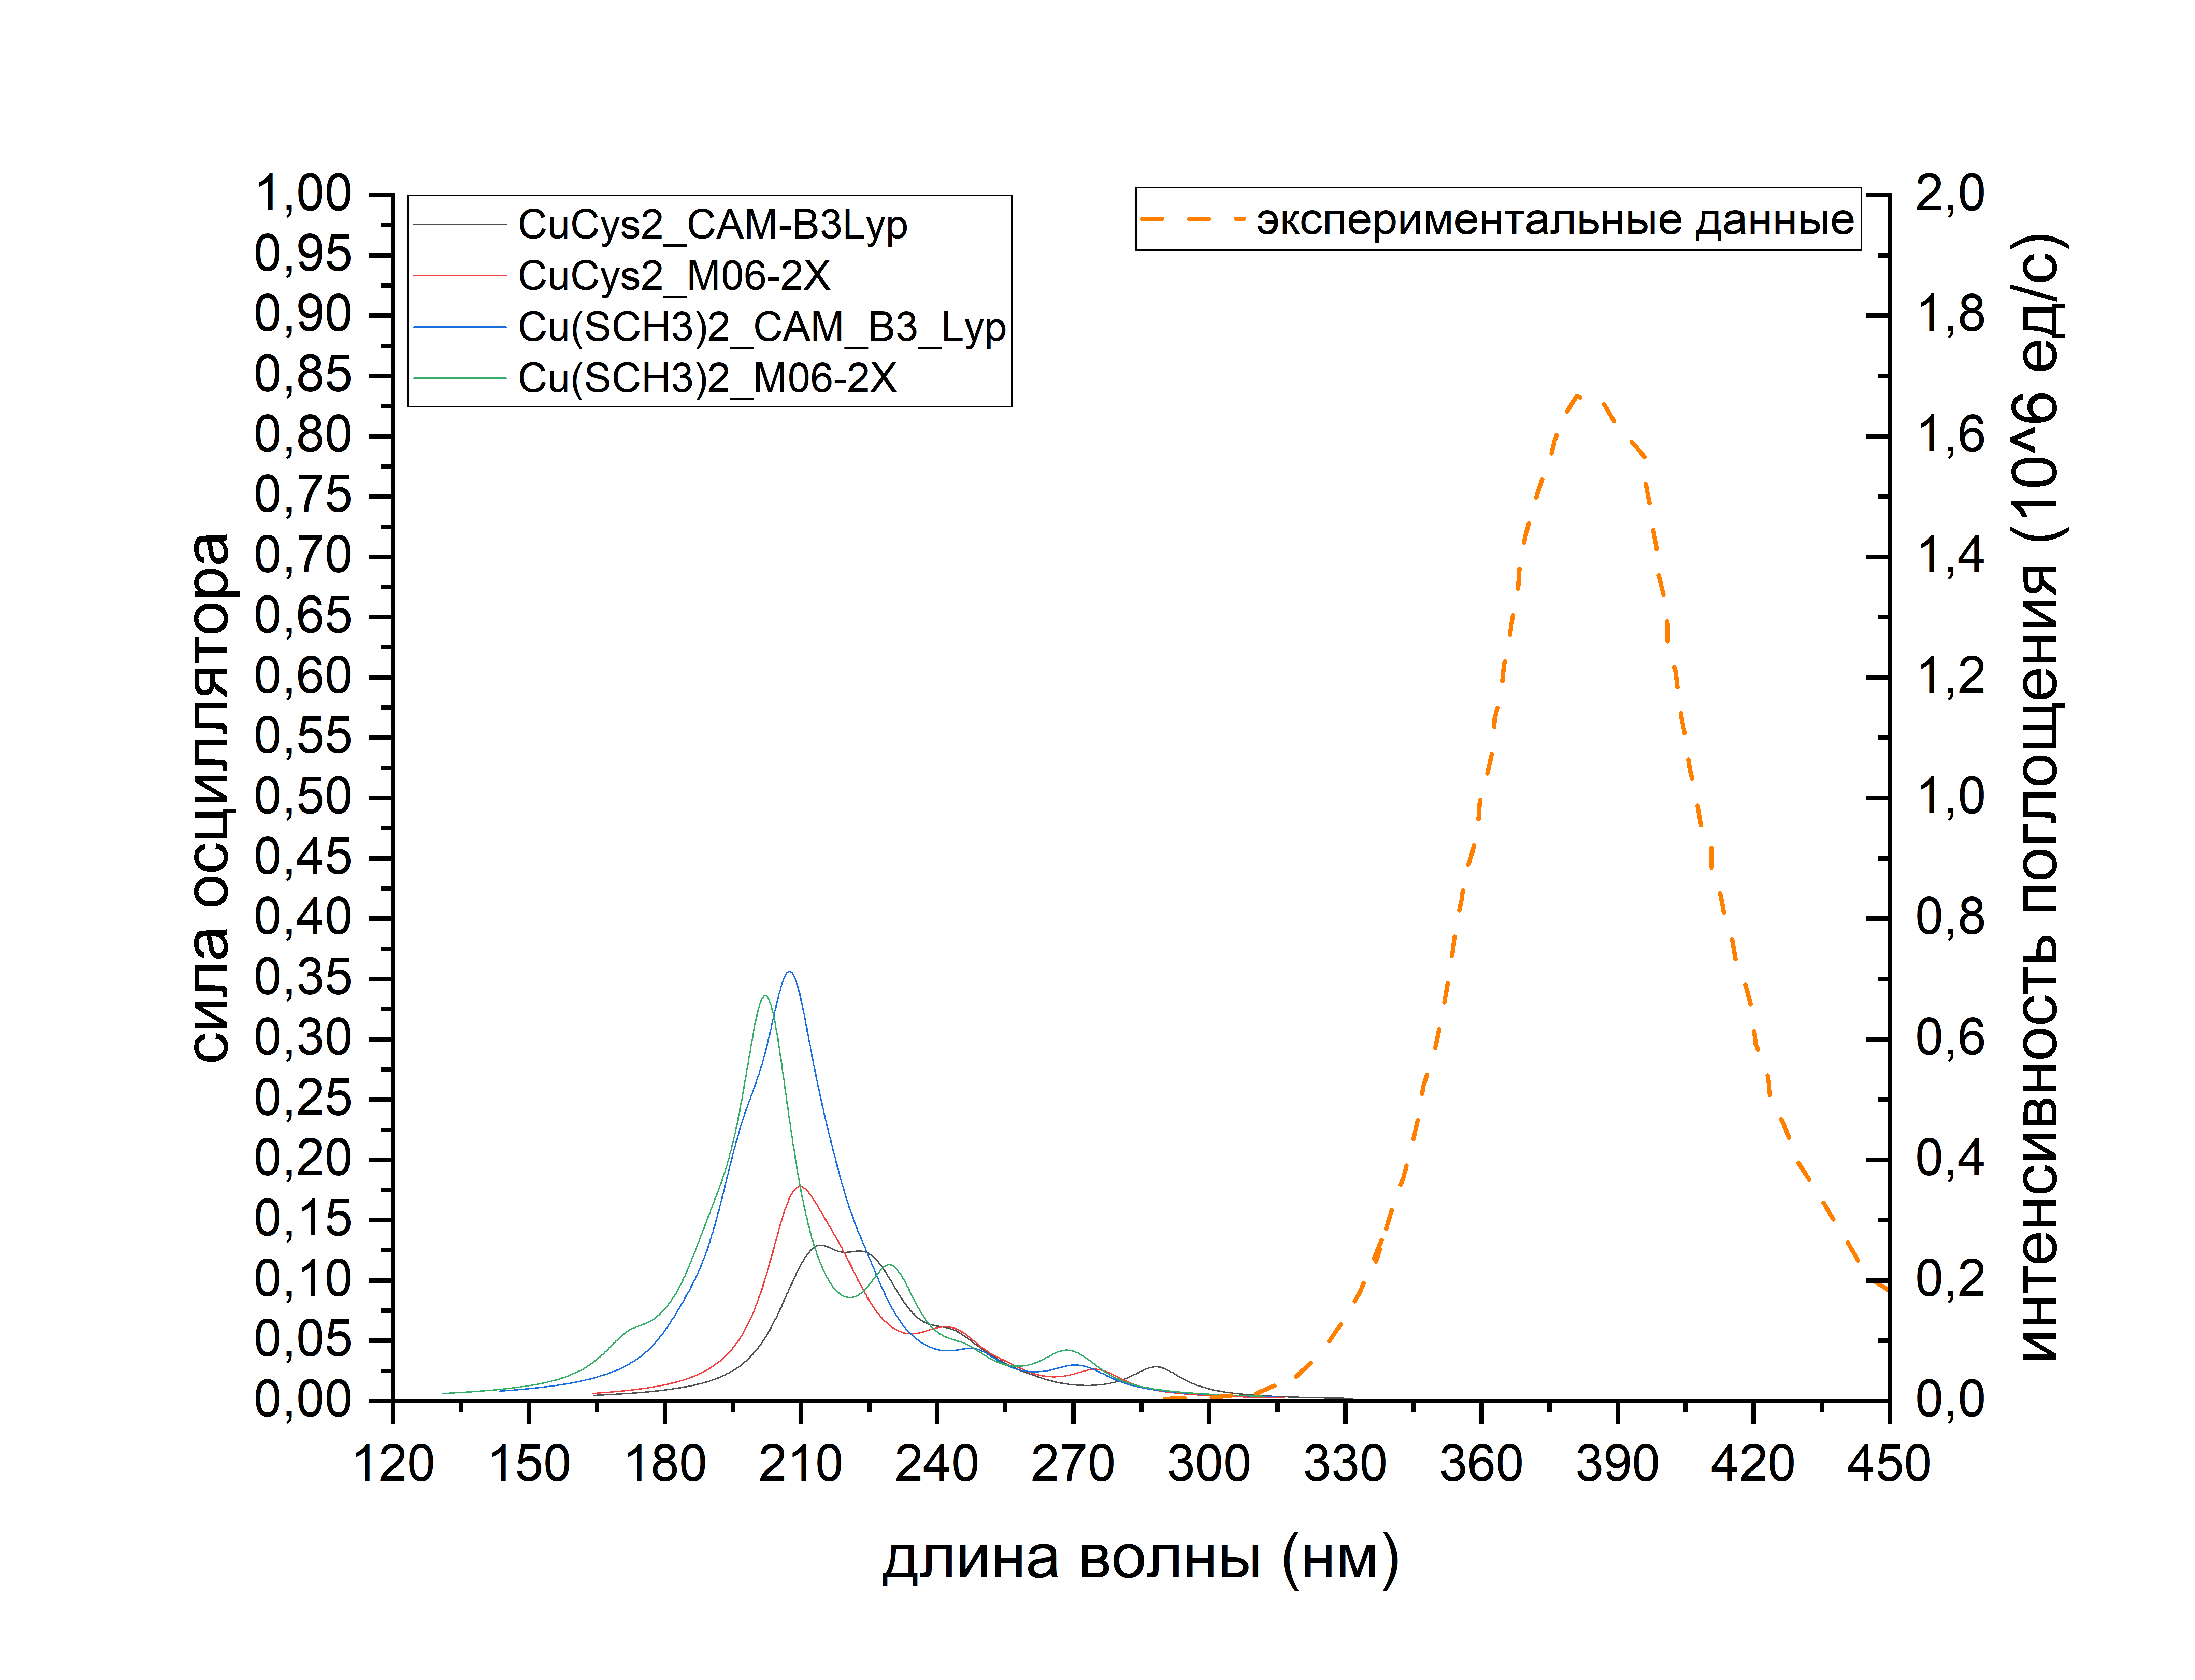
\includegraphics[frame, clip,width=0.49\columnwidth]{pictures/spectra/COMP_Cu_vacuum.png} }
		\subfloat[Комплекс \ce{[Cu2L2]^{-2}}]{ 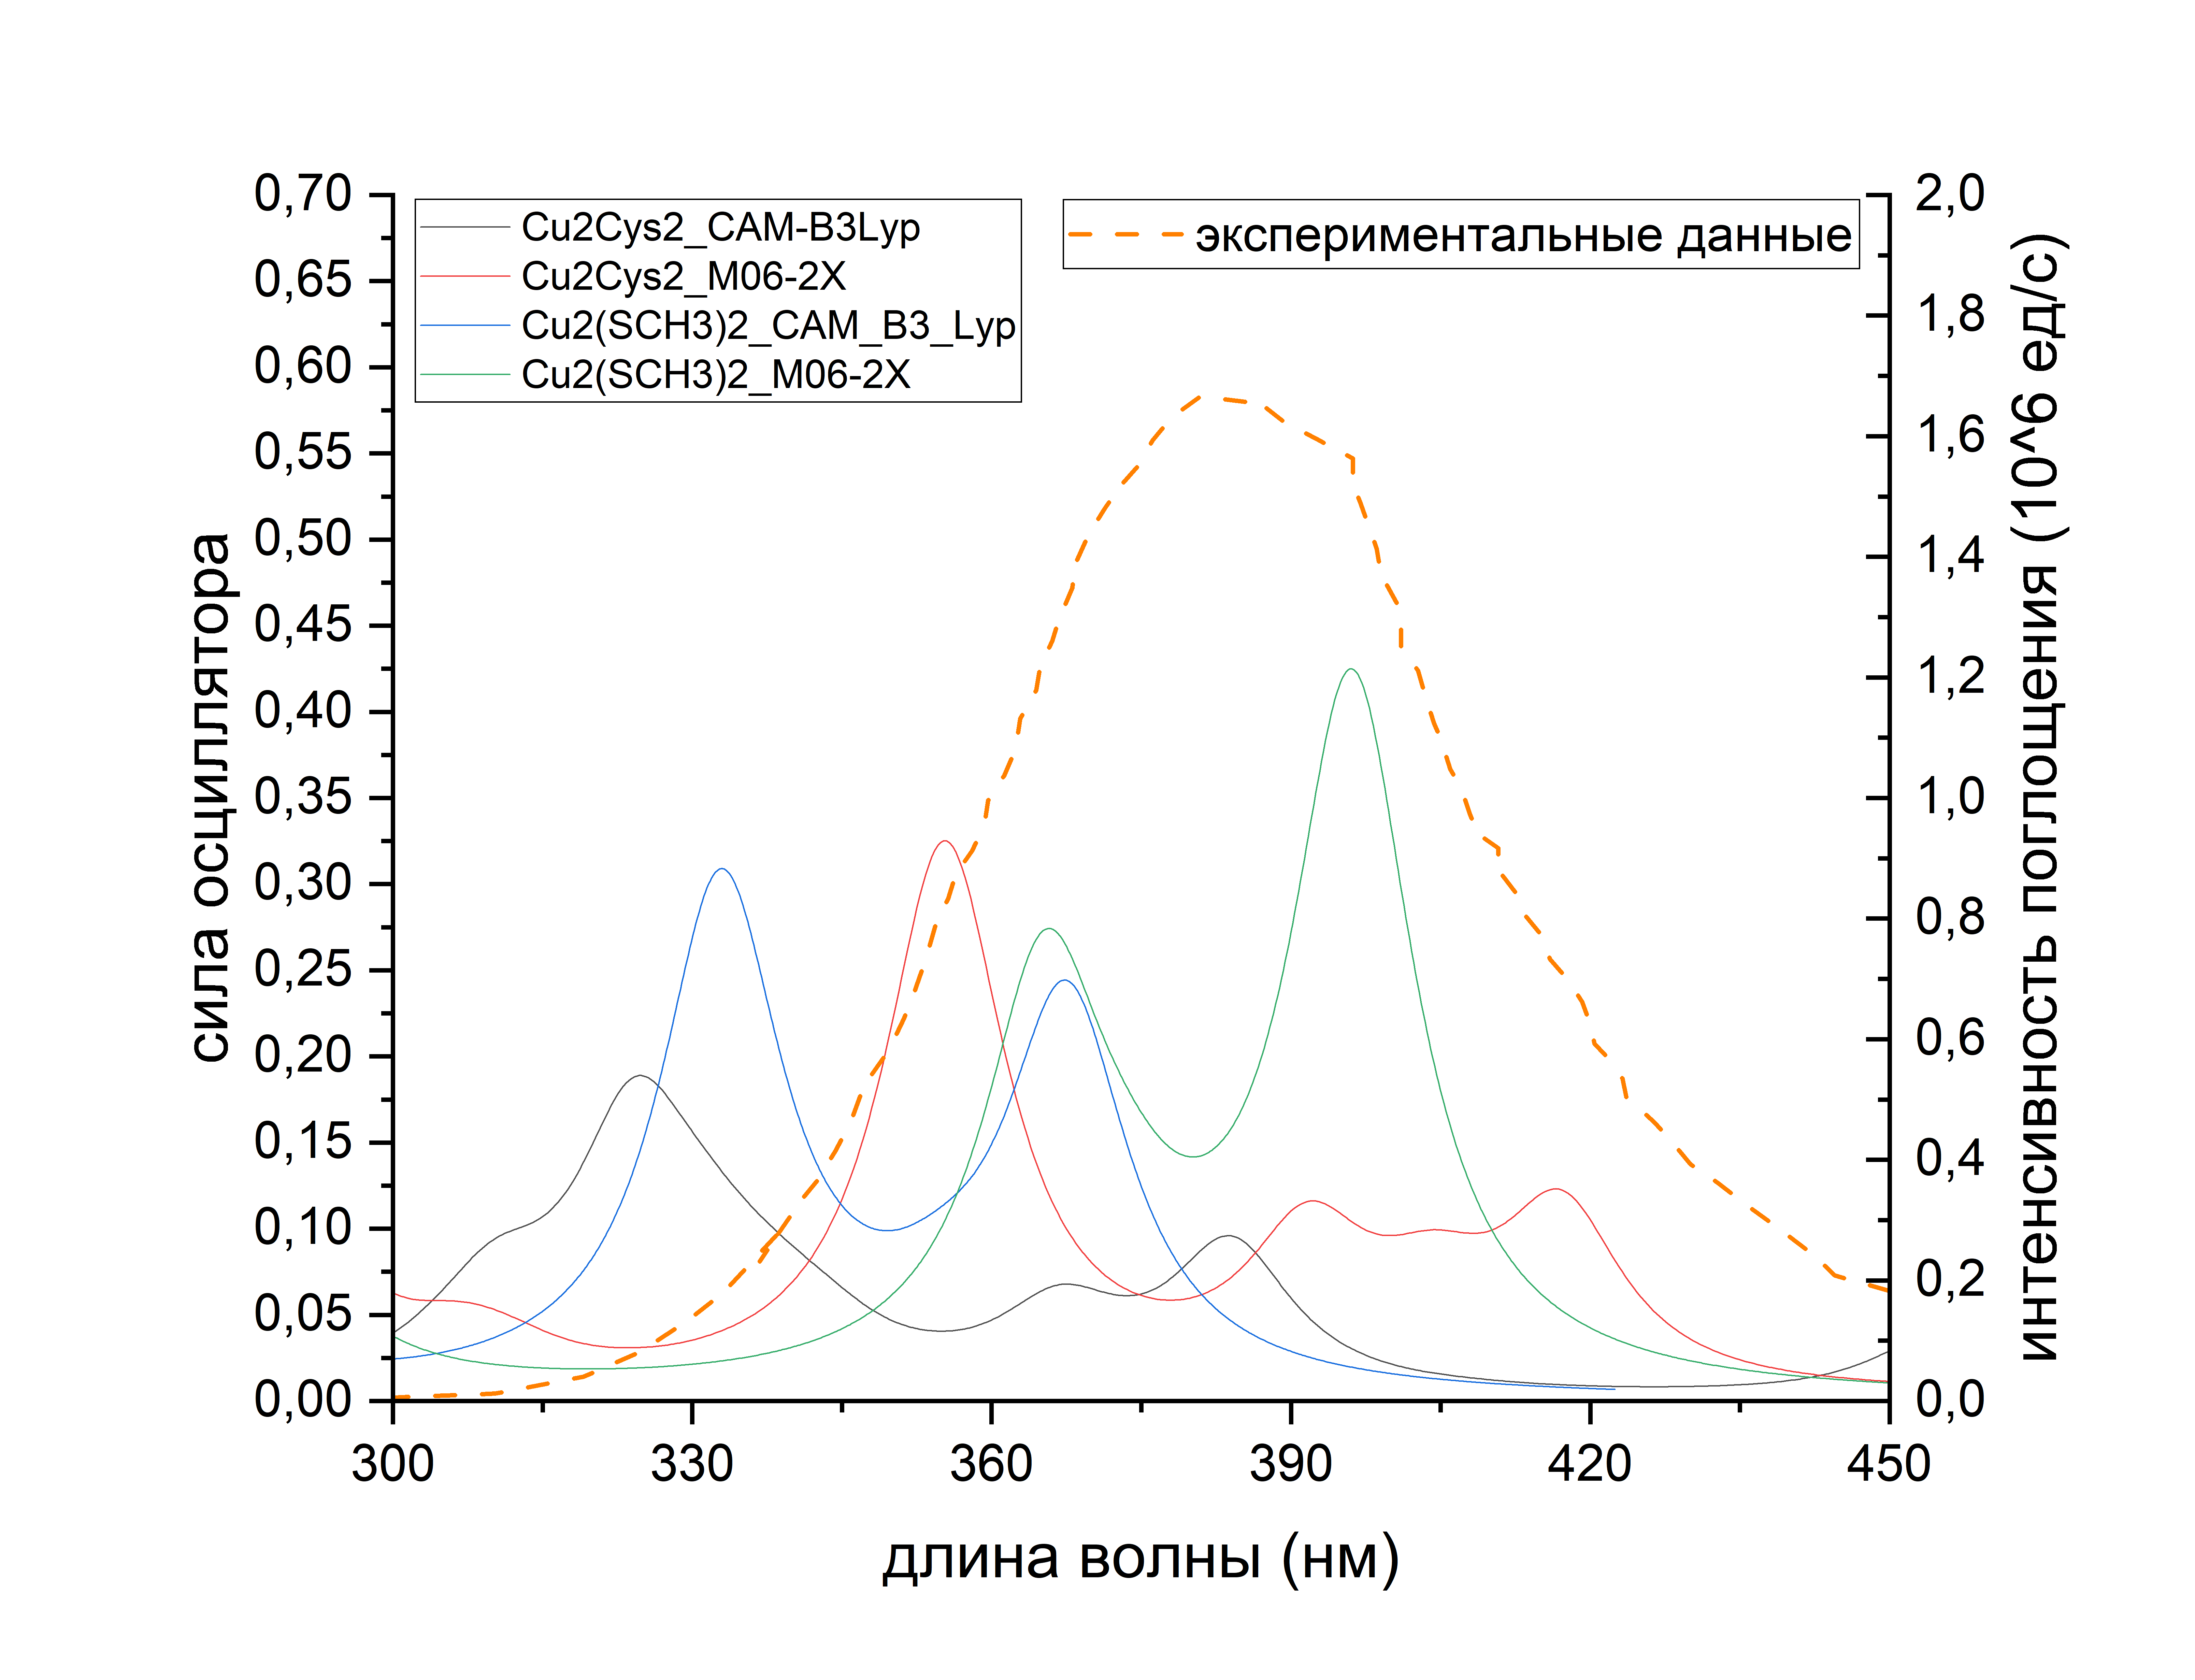
\includegraphics[frame, clip,width=0.49\columnwidth]{pictures/spectra/COMP_Cu2_vacuum.png}  }
		
		\subfloat[Комплекс \ce{[Cu3L2]^{-1}}]{ 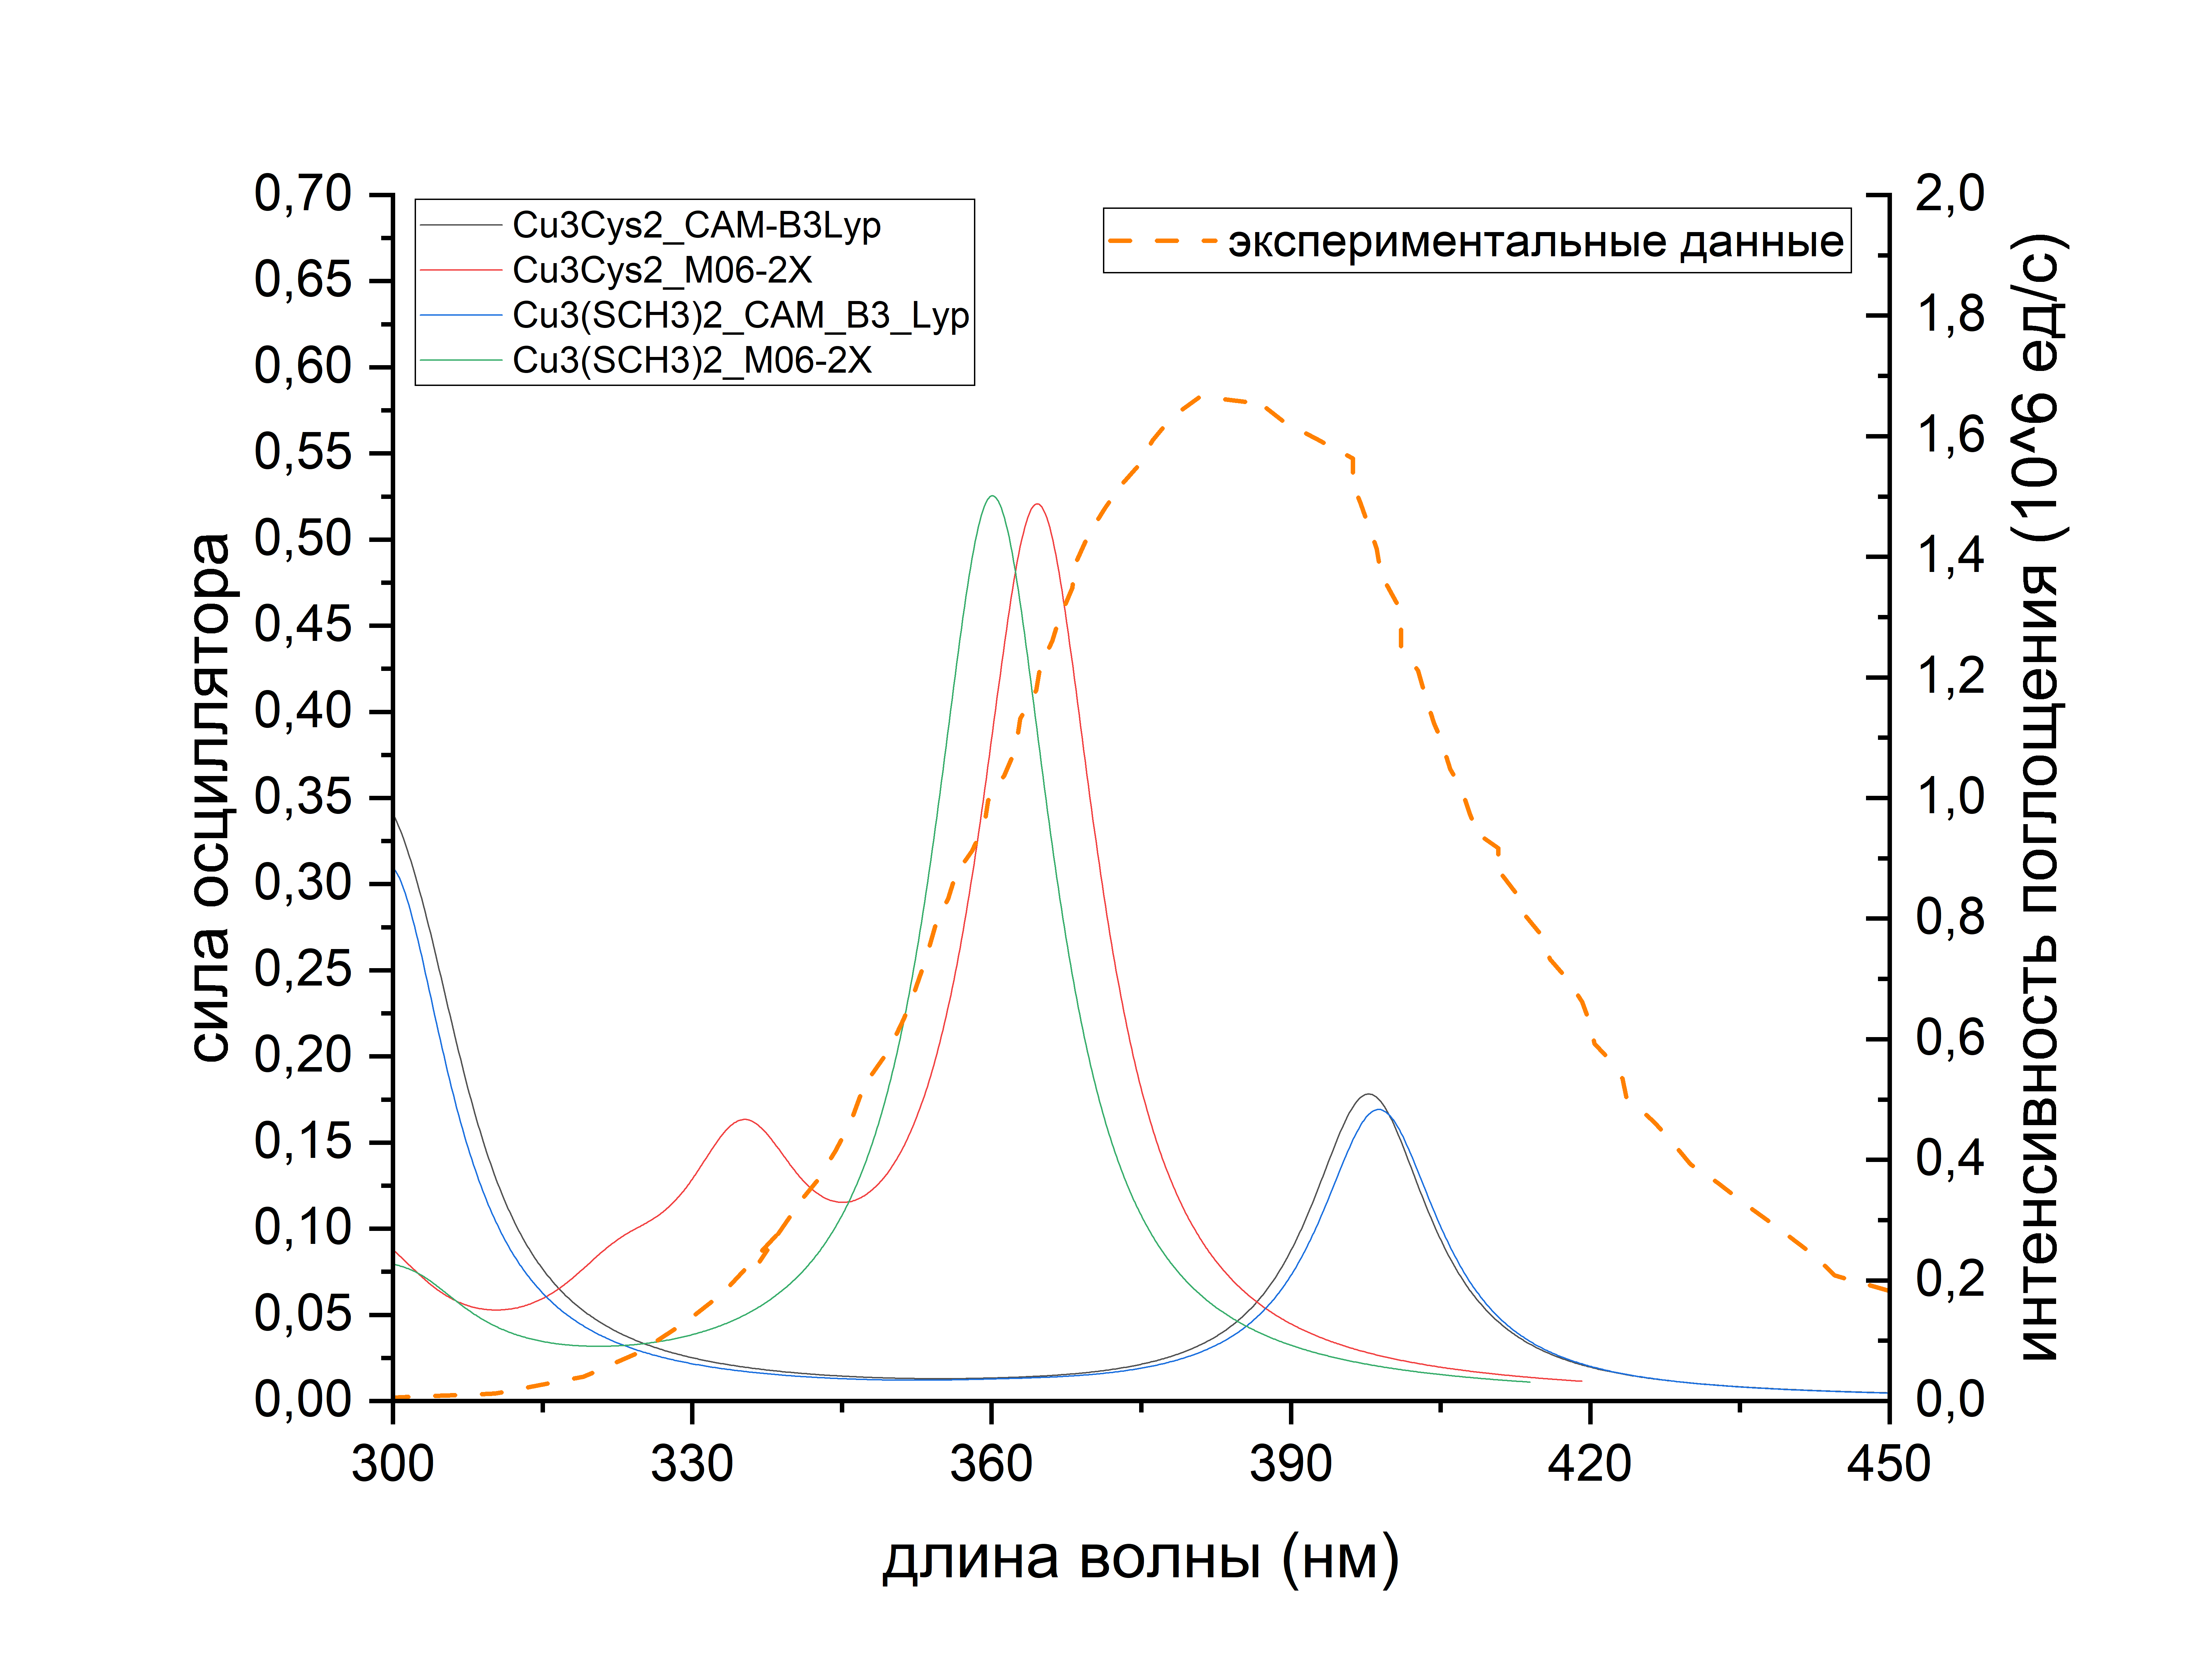
\includegraphics[frame, clip,width=0.49\columnwidth]{pictures/spectra/COMP_Cu3_vacuum.png}  }
		\subfloat[Комплекс \ce{[Cu4L3]^{-1}}]{ 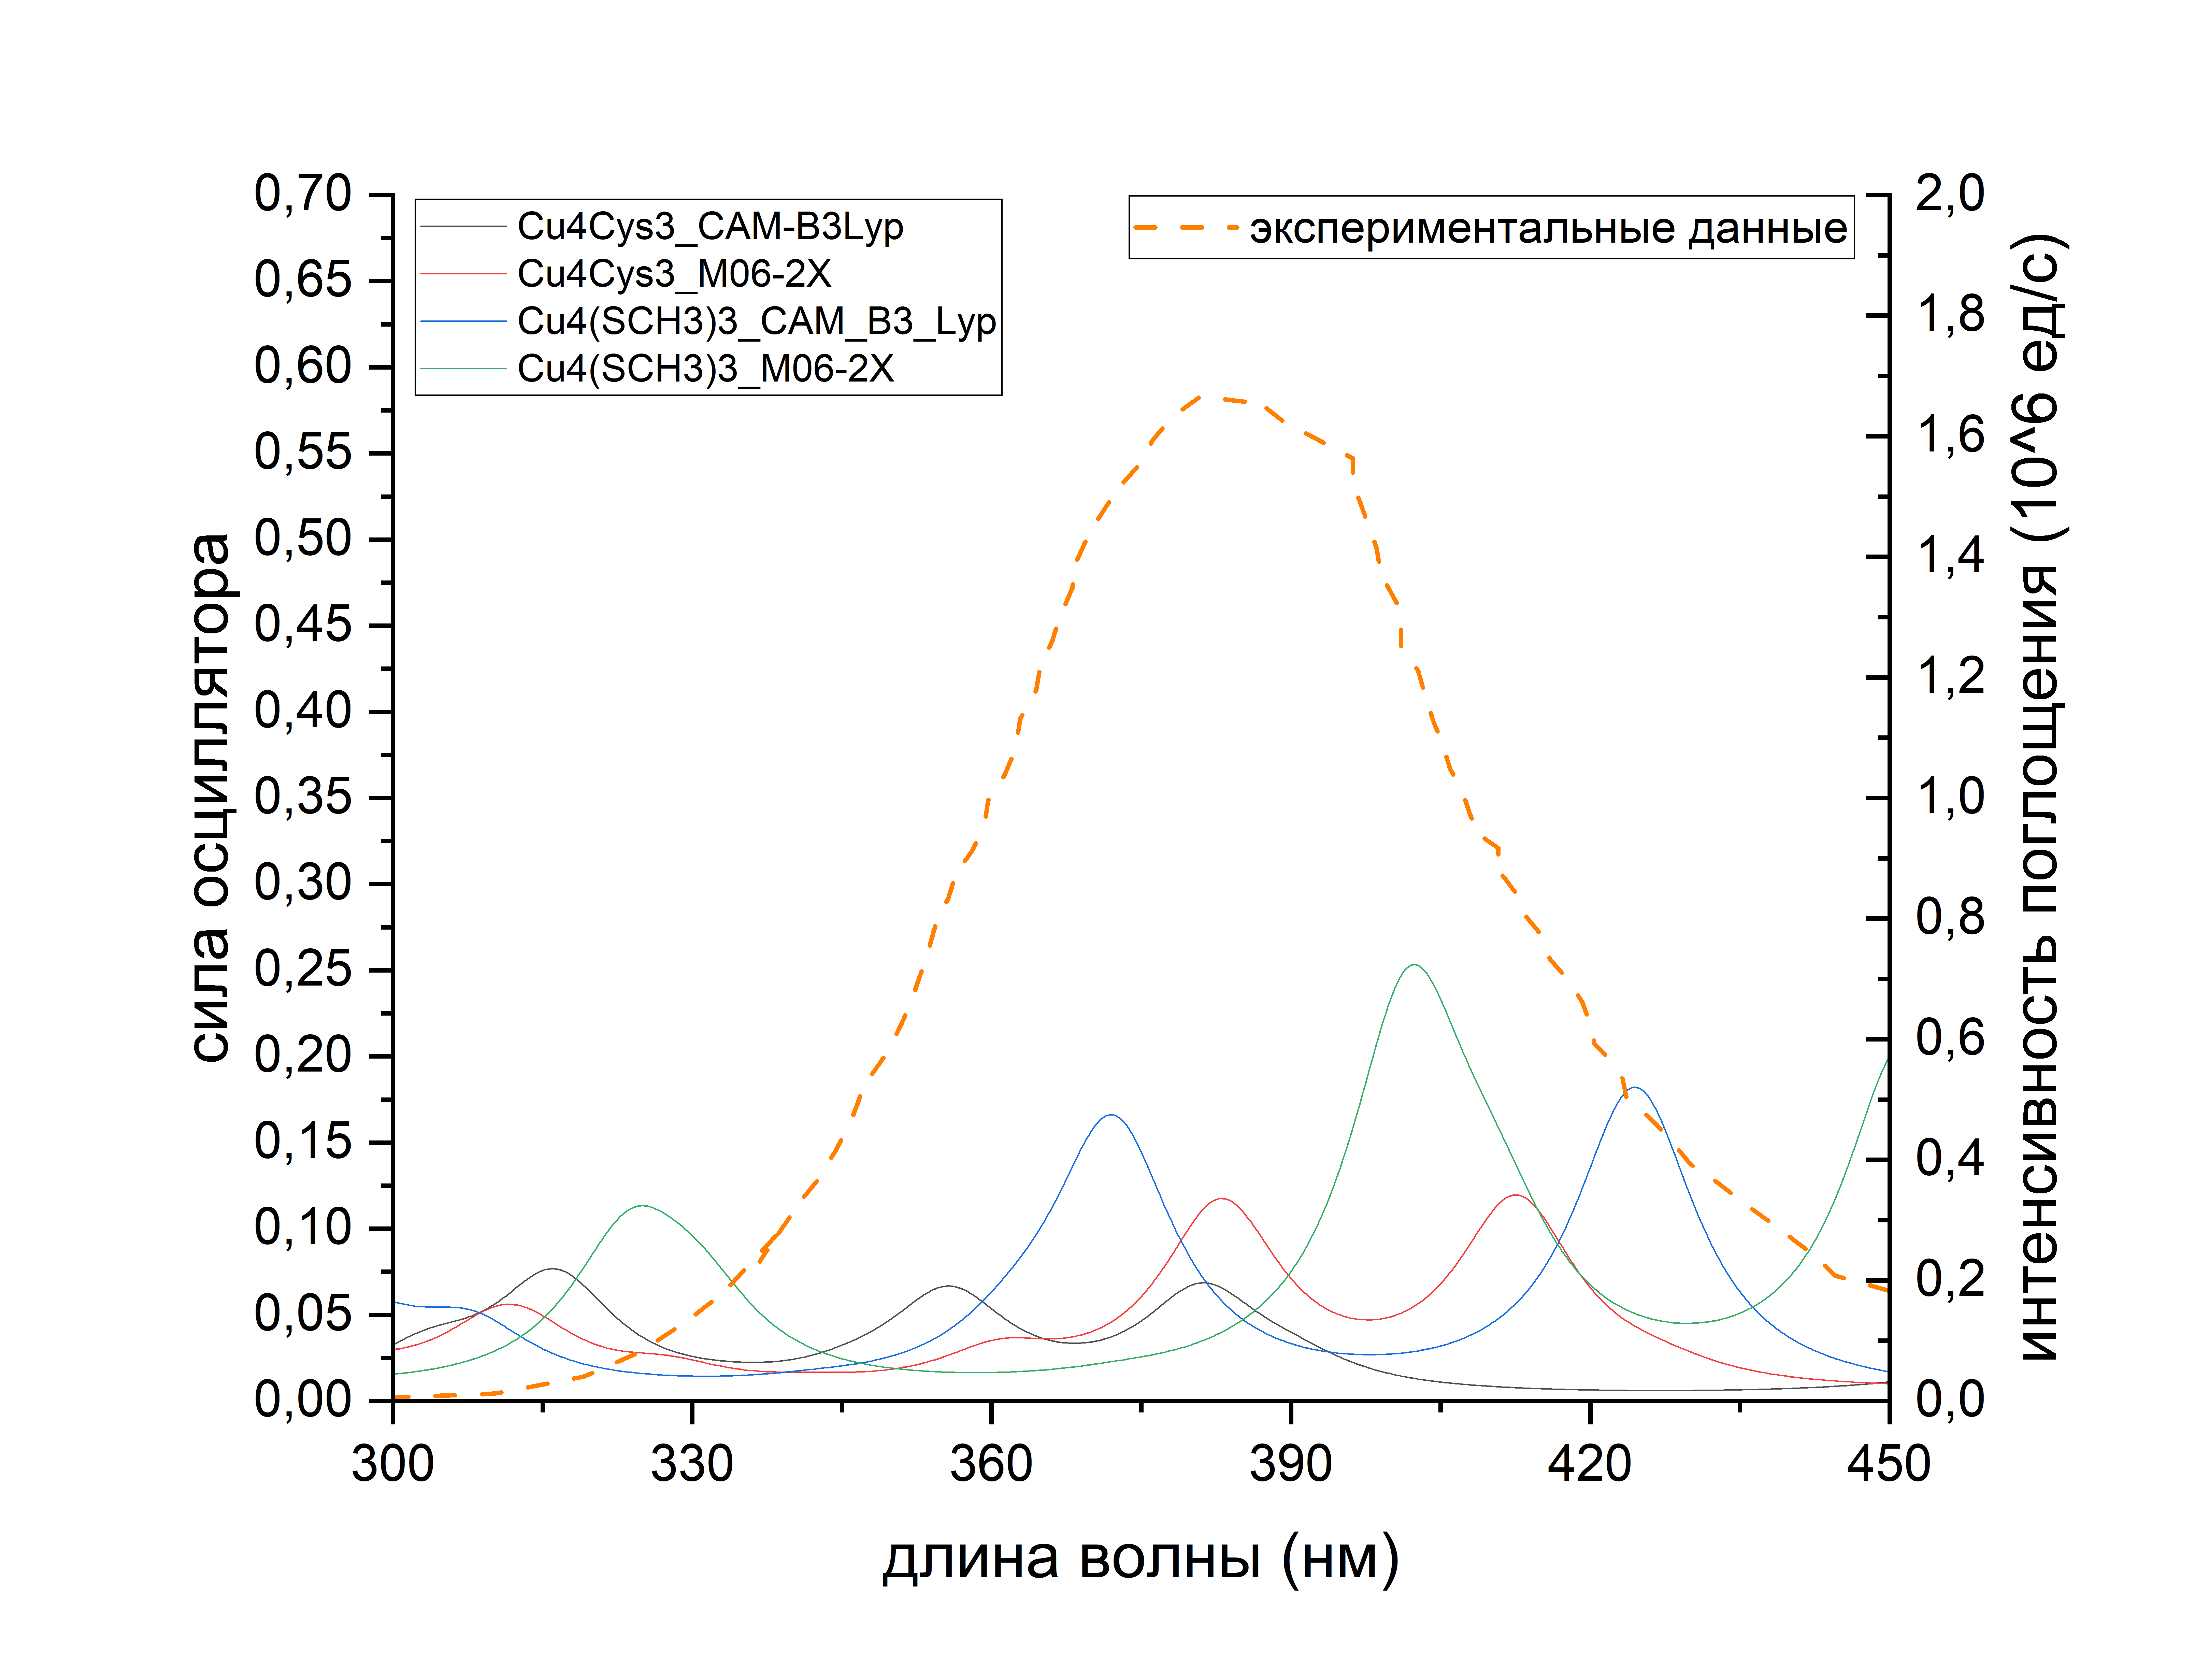
\includegraphics[frame, clip,width=0.49\columnwidth]{pictures/spectra/COMP_Cu4_vacuum.png}  }
		
		\subfloat[Комплекс \ce{[Cu5L4]^{-1}}]{ 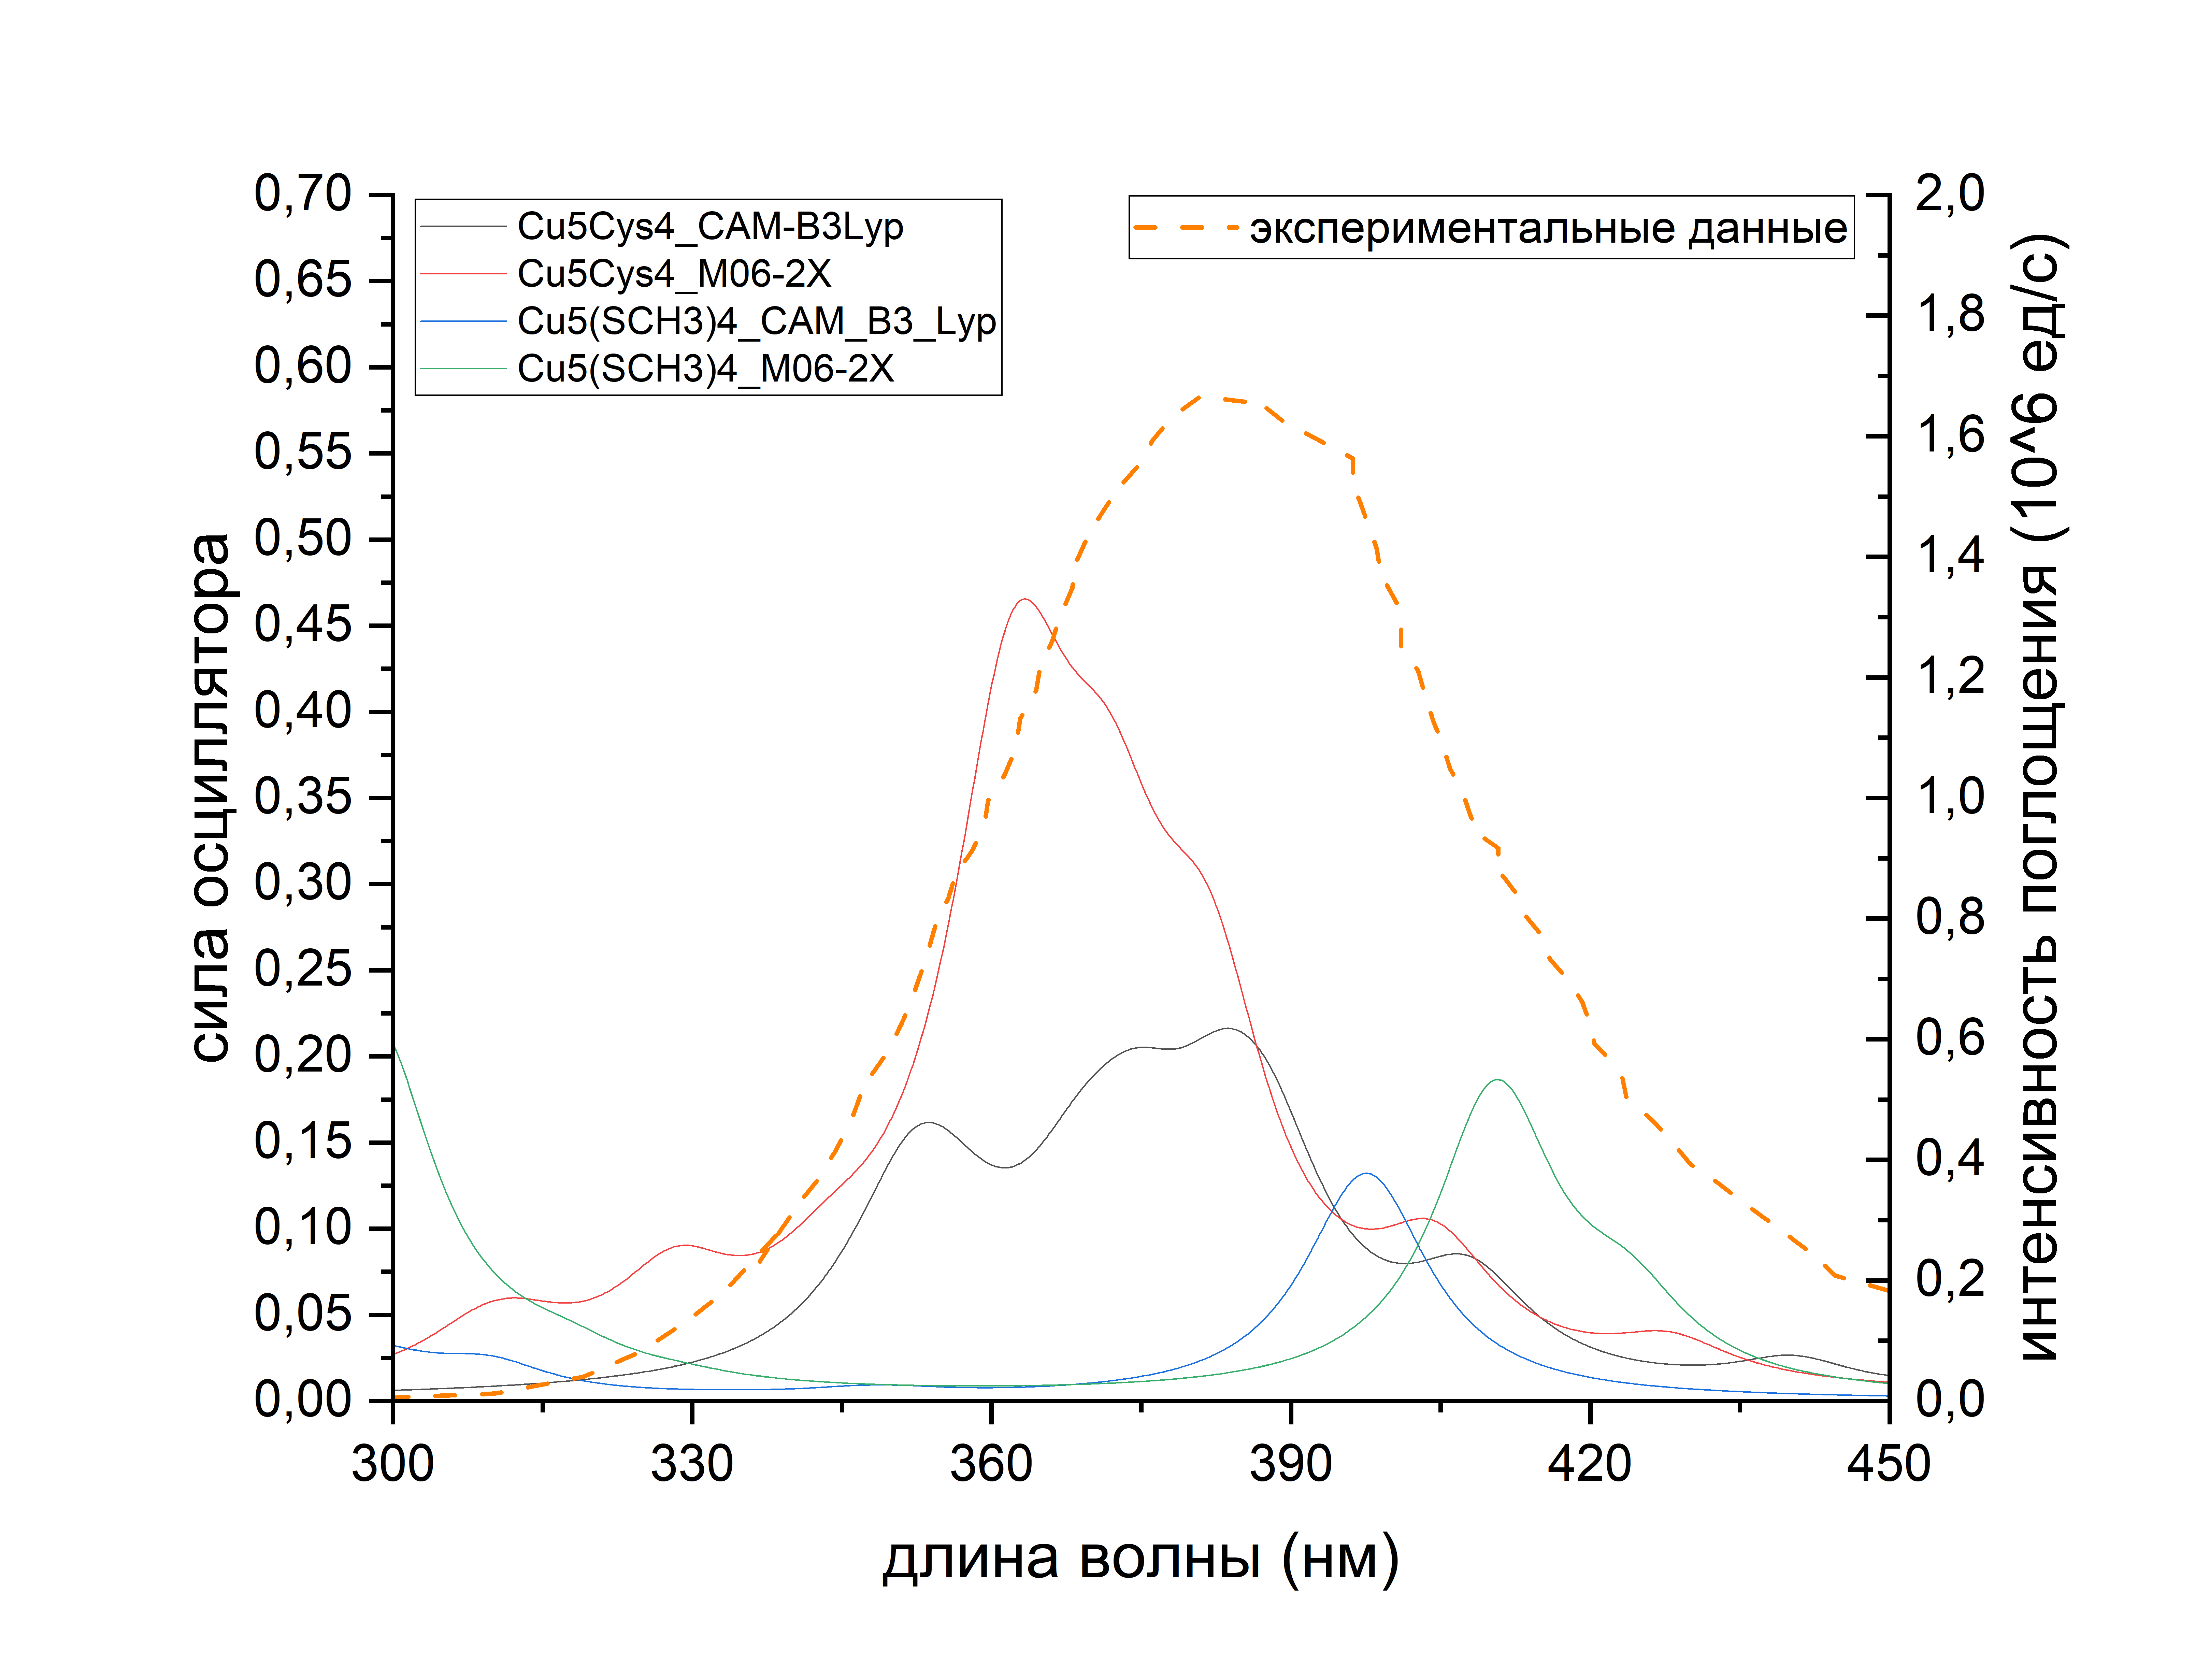
\includegraphics[frame, clip,width=0.49\columnwidth]{pictures/spectra/COMP_Cu5_vacuum.png}  }
		
		\caption{Сравнение спектров, полученных при помощи методов M06-2X/def2-TZVP и CAM-B3LYP/def2-TZVP для кластеров меди, стабилизированных \ce{SCH3} и \ce{Cys}, в газовой фазе.}
		\label{fig_vac_COMP}
	\end{figure}
	
%	\begin{figure}[H]
%		\centering
%		
%		\subfloat[Комплекс \ce{[CuL2]^{-1}}]{ 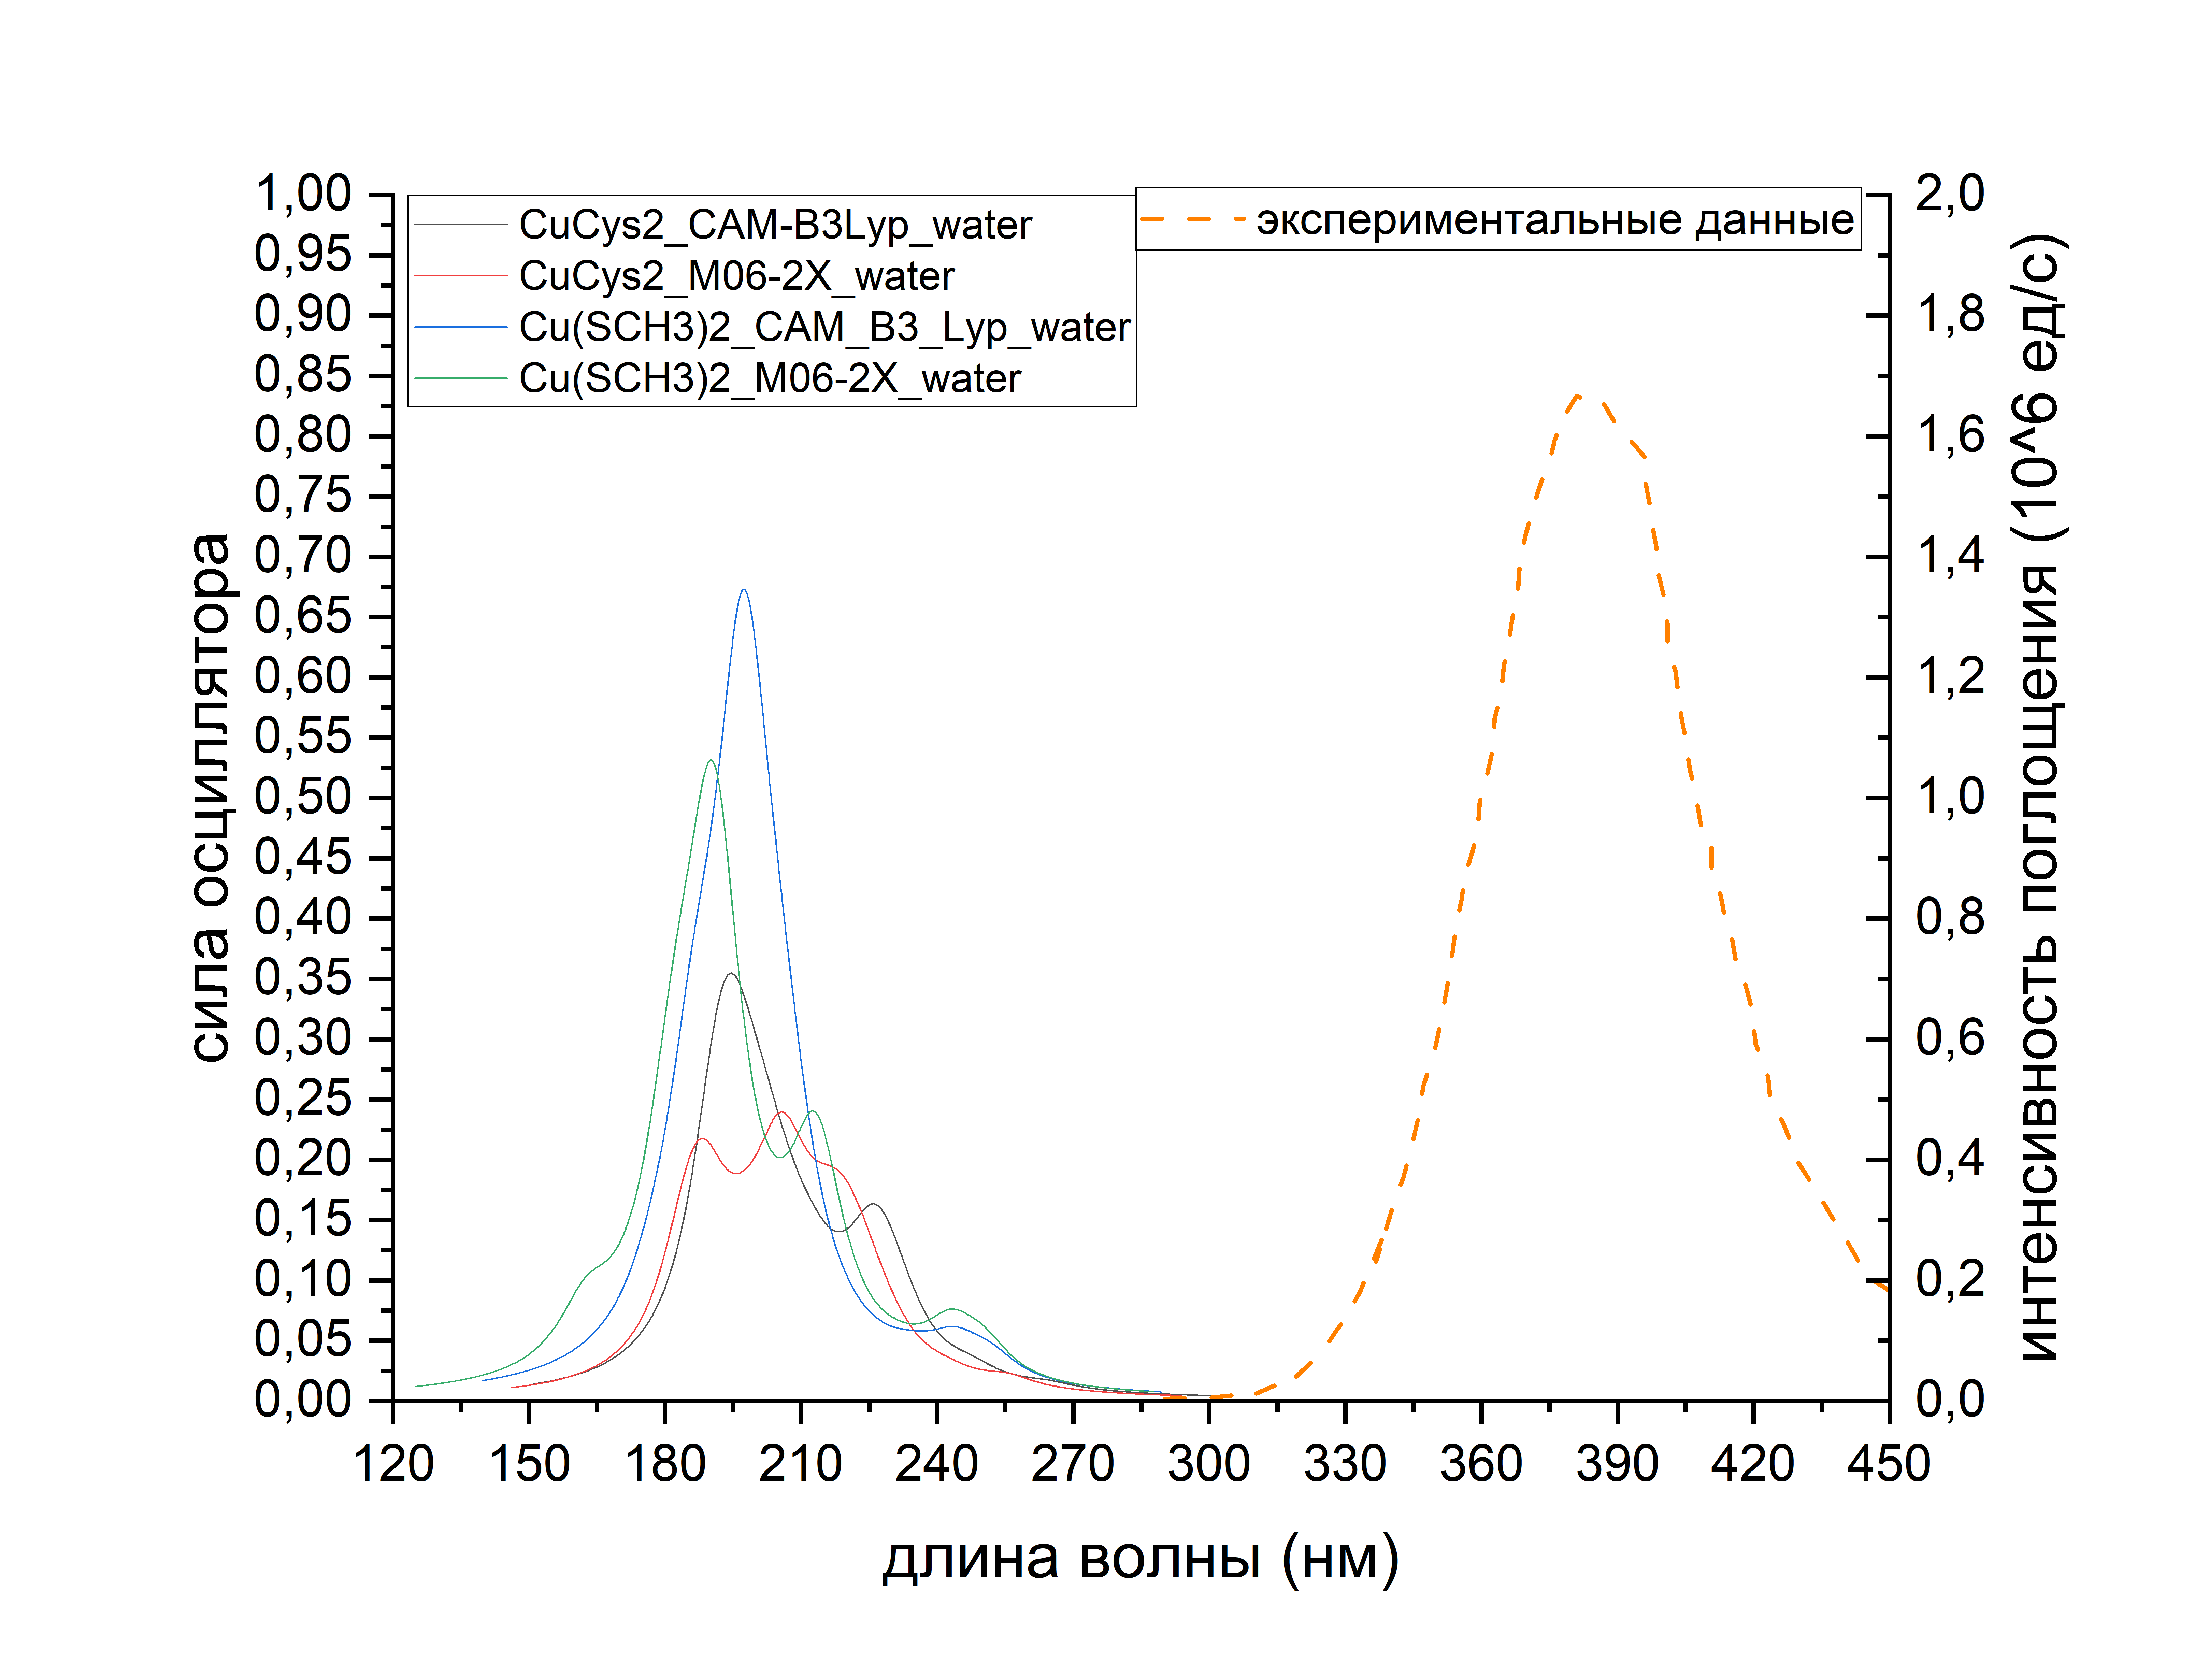
\includegraphics[frame, clip,width=0.49\columnwidth]{pictures/spectra/COMP_Cu_water.png} }
%		\subfloat[Комплекс \ce{[Cu2L2]^{-2}}]{ 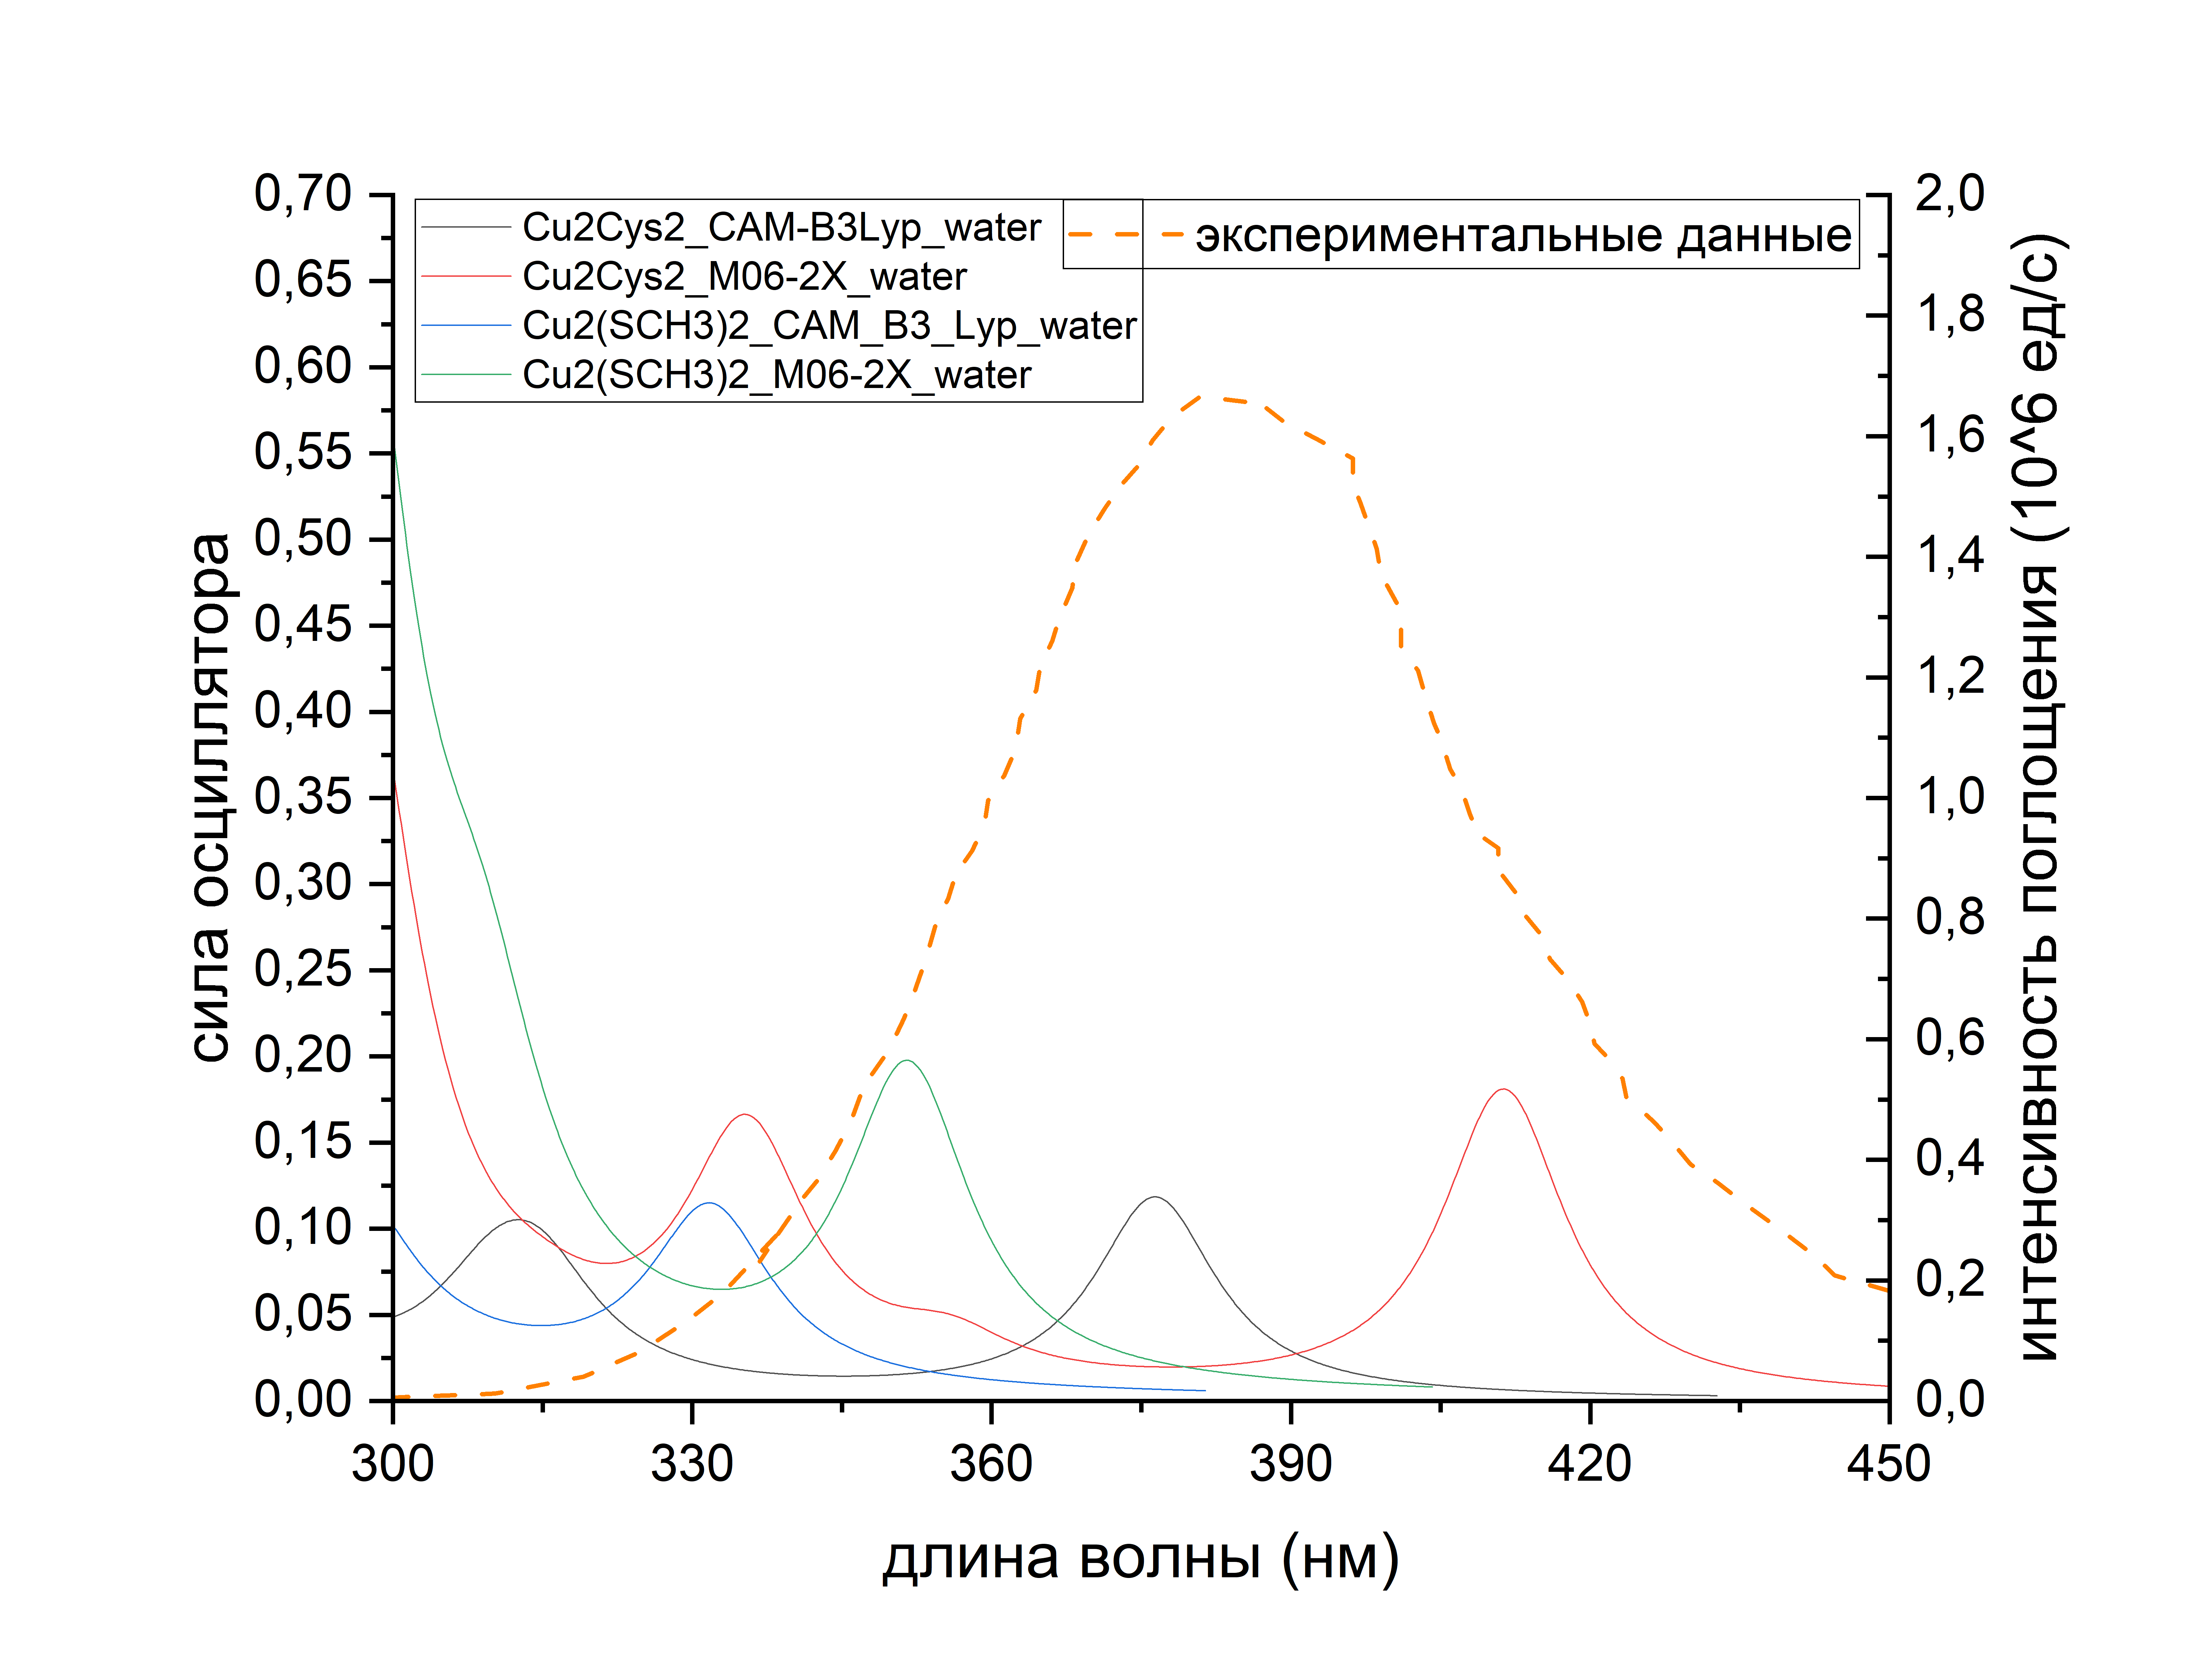
\includegraphics[frame, clip,width=0.49\columnwidth]{pictures/spectra/COMP_Cu2_water.png}  }
%		
%		\subfloat[Комплекс \ce{[Cu3L2]^{-1}}]{ 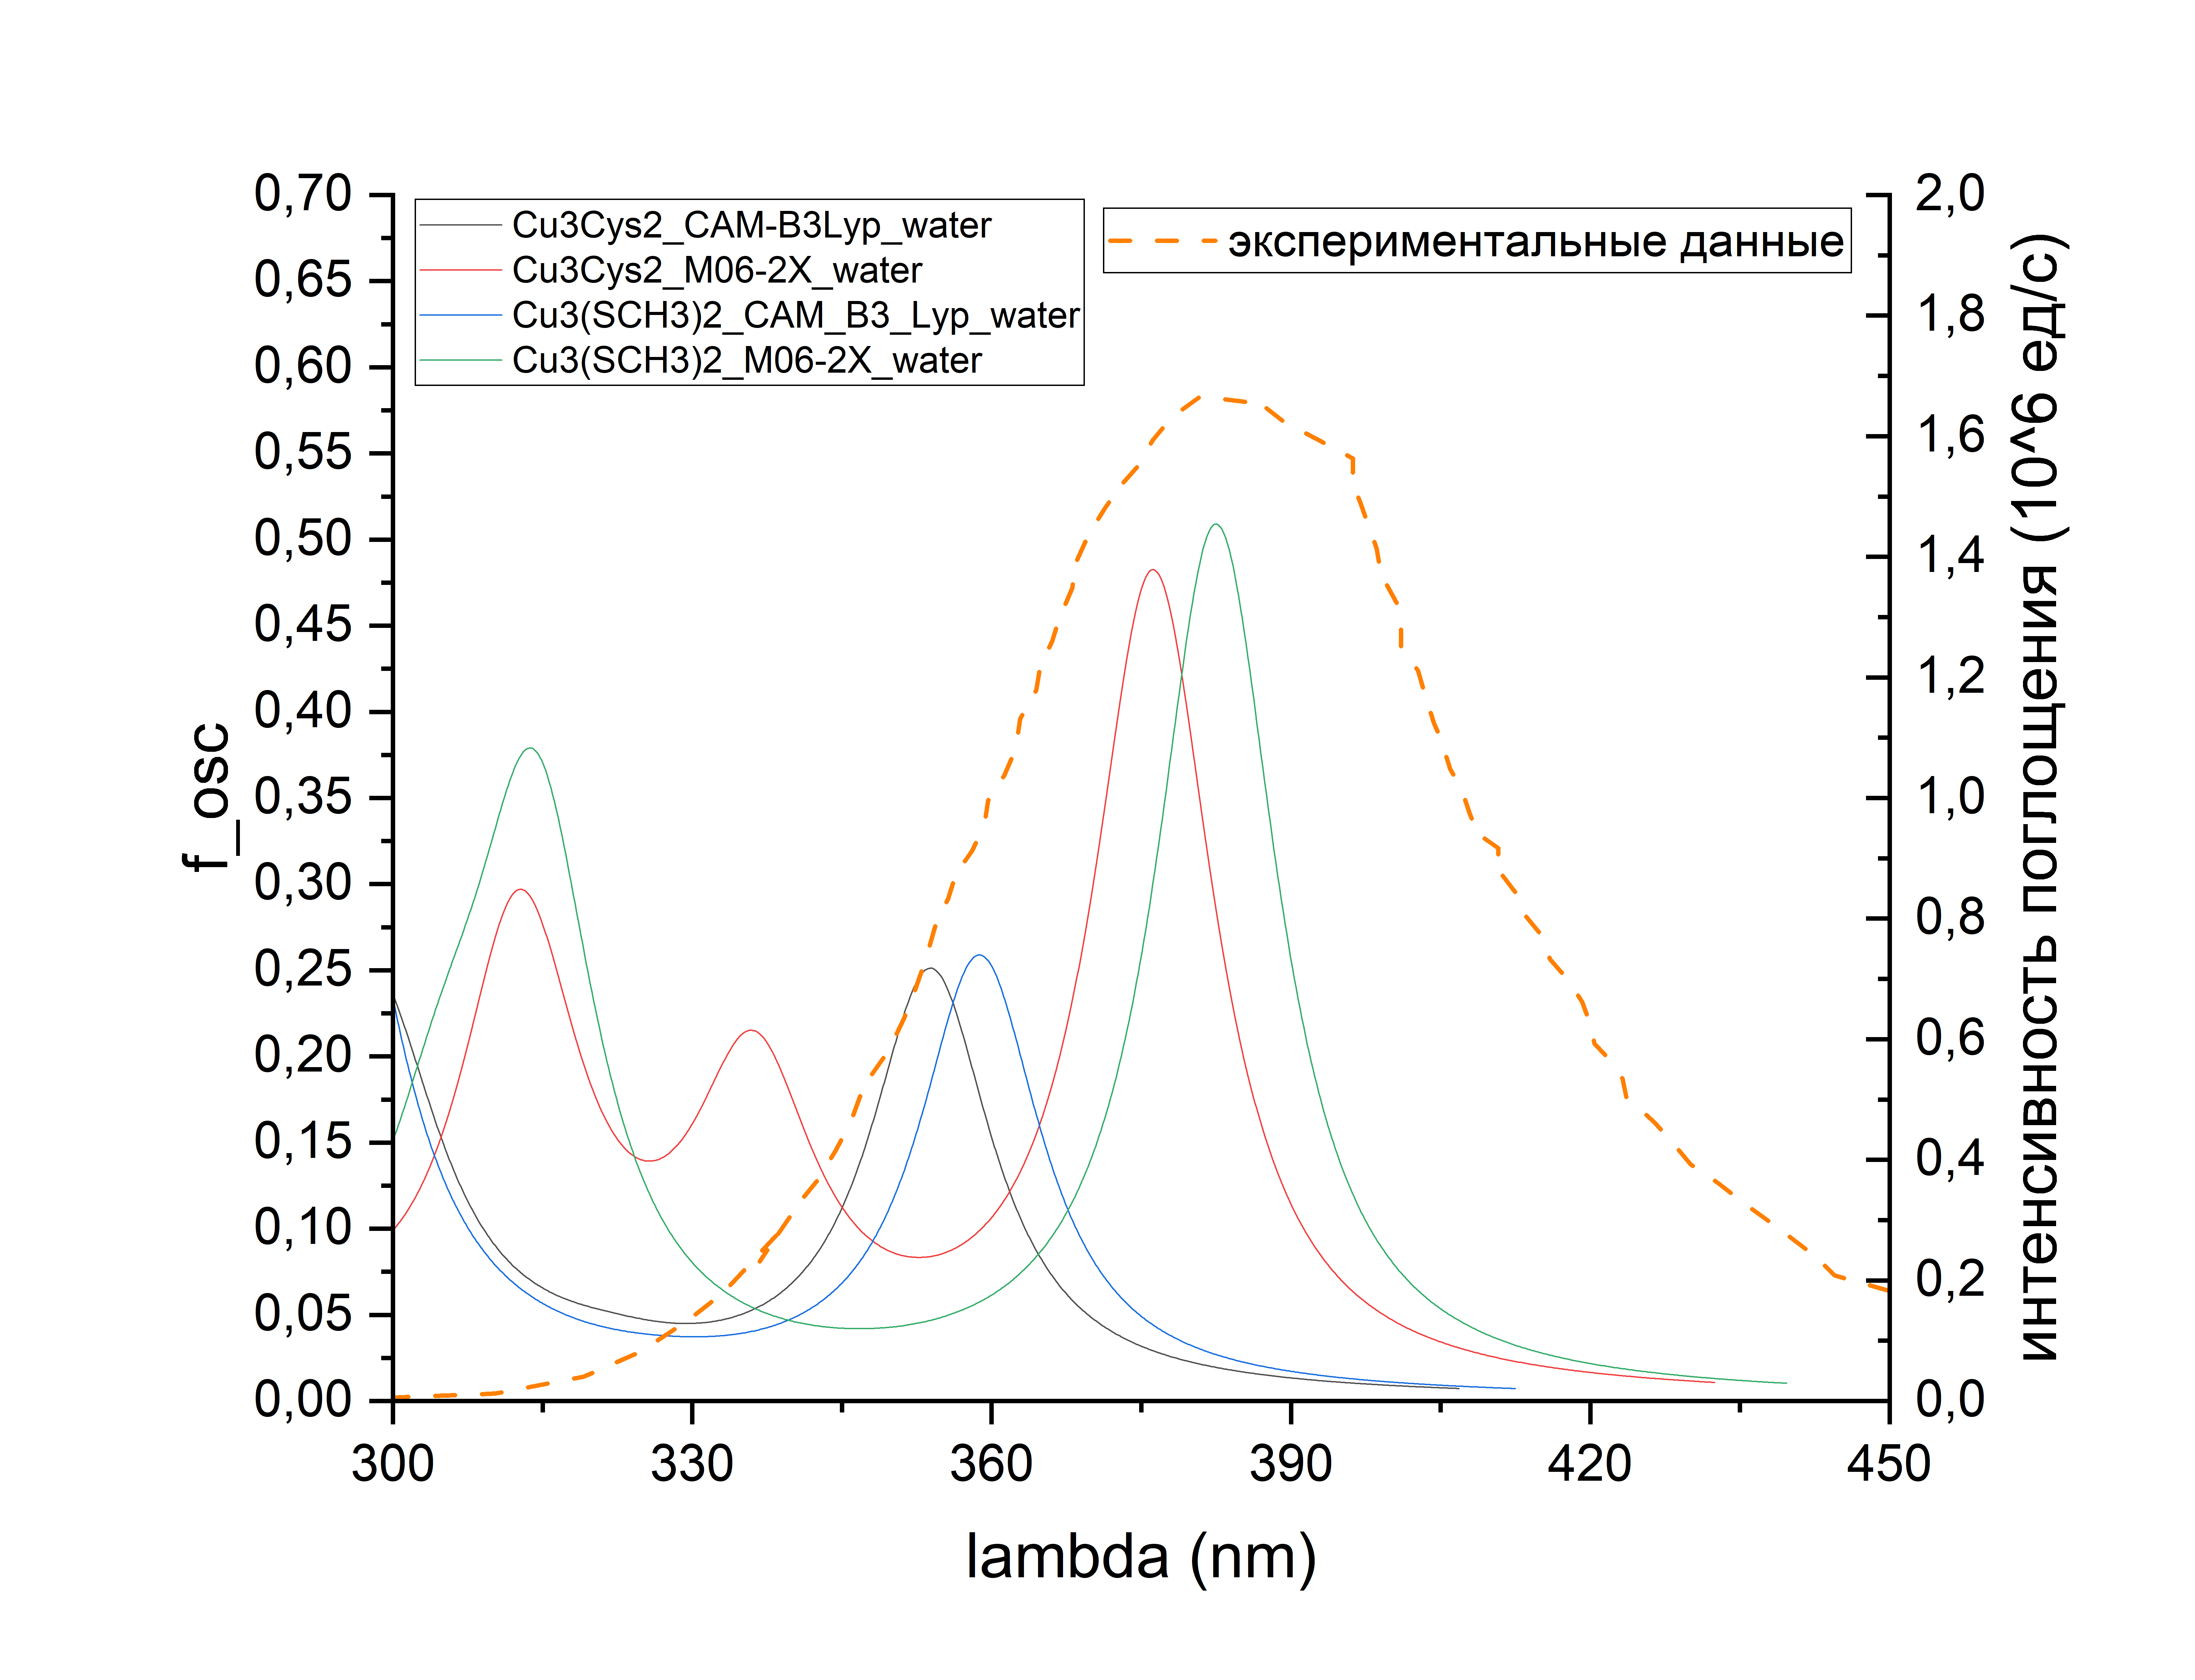
\includegraphics[frame, clip,width=0.49\columnwidth]{pictures/spectra/COMP_Cu3_water.png}  }
%		\subfloat[Комплекс \ce{[Cu4L3]^{-1}}]{ 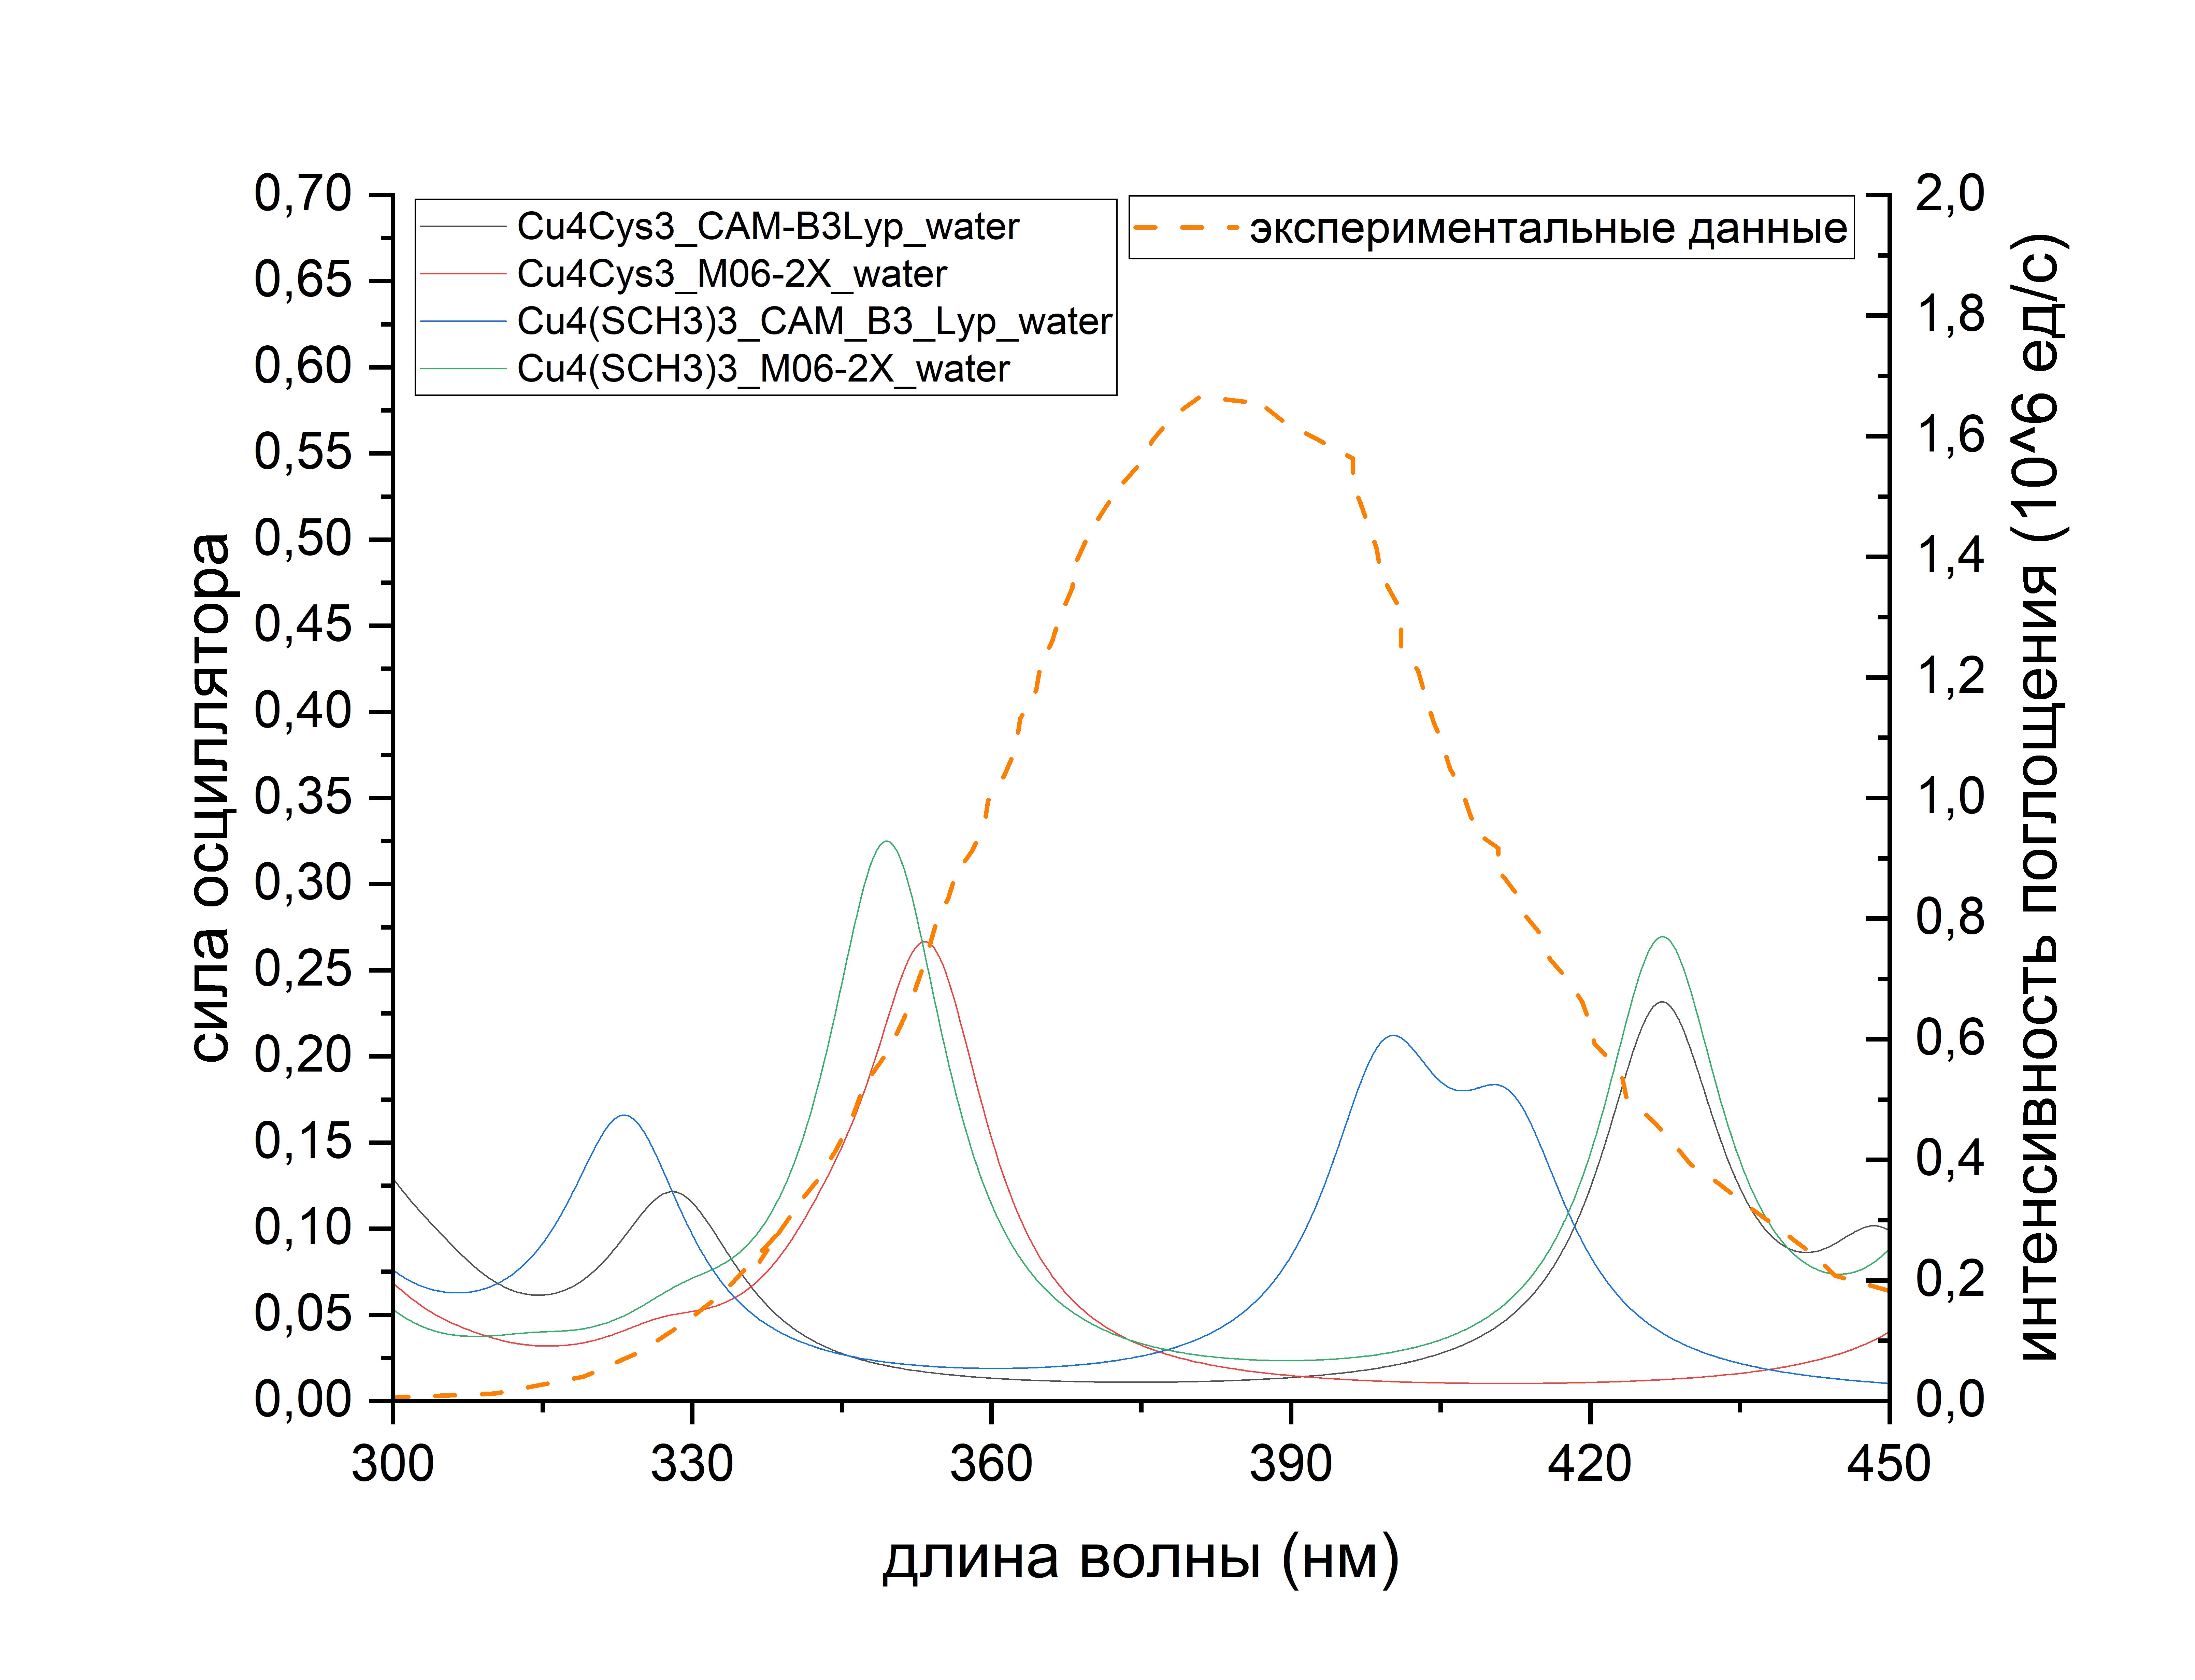
\includegraphics[frame, clip,width=0.49\columnwidth]{pictures/spectra/COMP_Cu4_water.png}  }
%		
%		\caption{Сравнение спектров, полученных при помощи методов M06-2X/def2-TZVP и CAM-B3LYP/def2-TZVP для кластеров меди, стабилизированных \ce{SCH3} и \ce{Cys}, в воде.}
%		\label{fig_wat_COMP}
%	\end{figure}

	\newpage
	
	\section*{Заключение}
	\addcontentsline{toc}{section}{ЗАКЛЮЧЕНИЕ}
	
%	В ходе работы проведено теоретическое исследование нанокластеров меди, стабилизированных тиолятами. Исследованы следующие структуры: \ce{[CuL2]^{-1}}, \ce{[Cu2L2]^{-2}}, \ce{[Cu3L2]^{-1}}, \ce{[Cu4L3]^{-1}} и \ce{[Cu5L4]^{-1}}. В качестве лиганда использованы метилтиогруппа \ce{SCH3} и цистеин \ce{Cys}. Расчёты проведены в газовой фазе и в воде (модель CPCM).
%	
%	Первыми изучены комплексы с \ce{L=SCH3}. После минимизации геометрий при помощи метода теории возмущений Мёллера-Плессета второго порядка (MP2/def2-TZVP), были расчитаны модельные спектры поглощения на оптимизированных геометриях. В качестве высокоуровневого метода выбран метод связанных кластеров с учетом однократных и двухкратных возбуждений — EOM-CCSD. На основании спектров поглощения, полученных этим методом, проведён бенчмаркинг пяти DFT функционалов:  BHandHLYP, CAM-B3LYP, M06-2X, PBE0 и wB97X. Для тестирования функционалов были использованы комплексы \ce{[CuL2]^{-1}} и \ce{[Cu2L2]^{-2}}. По итогам банчмарка установлено, что метод CAM-B3LYP лучше всего согласуется с эталонным EOM-CCSD. В то же время, метод M06-2X даёт лучшее согласование с экспериментальными данными. 
%	
%	Вторыми рассчитаны спектры поглощения нанокластеров меди, стабилизированных цистеином. Геометрии комплексов также были оптимизированны в газовой фазе и в воде методом MP2/def2-TZVP. Для оптимизированных комплексов получены модельные спектры поглощения при помощи методов CAM-B3LYP и M06-2X. 

	В ходе данной работы проведено теоретическое исследование нанокластеров меди, стабилизированных тиолятными лигандами. В рамках исследования были рассмотрены следующие структуры: \ce{[CuL2]^{-1}}, \ce{[Cu2L2]^{-2}}, \ce{[Cu3L2]^{-1}}, \ce{[Cu4L3]^{-1}} и \ce{[Cu5L4]^{-1}}, что позволило охватить широкий диапазон кластеров различной размерности и координации. В качестве лигандов выбраны метилтиогруппа \ce{SCH3} и цистеин \ce{Cys}, что дало возможность проанализировать влияние как относительно простой, так и более сложной био-тиолятной системы. Все расчёты проводились как в газовой фазе, так и с учётом растворителя (вода) с использованием модели непрерывной поляризуемой среды CPCM.

	На первом этапе были подробно изучены комплексы с лигандом \ce{L=SCH3}. После оптимизации геометрий с применением метода теории возмущений Мёллера–Плессета второго порядка (MP2/def2-TZVP) были рассчитаны модельные спектры поглощения на полученных оптимизированных структурах. В качестве эталонного высокоуровневого подхода был выбран метод связанных кластеров с учётом однократных и двукратных возбуждений (EOM-CCSD), позволяющий с высокой точностью описывать возбужденные состояния. На основе спектров, полученных данным методом, был проведён бенчмаркинг пяти DFT-функционалов: BHandHLYP, CAM-B3LYP, M06-2X, PBE0 и wB97X. 

	По результатам проведённого бенчмаркинга установлено, что функционал CAM-B3LYP демонстрирует наилучшее согласование с эталонными расчётами уровня EOM-CCSD, что делает его предпочтительным с точки зрения воспроизведения теоретических данных. В то же время функционал M06-2X обеспечивает более хорошее соответствие экспериментальным спектрам поглощения, что указывает на его практическую применимость при интерпретации экспериментальных результатов. Метод BHandH-LYP показал себя даже более пригодным для оценки энергии перехода HOMO\ths $\rarr$\ths LUMO, чем M06-2X, хотя в среднем дал результаты хуже.к 

	%	На следующем этапе были рассчитаны спектры поглощения нанокластеров меди, стабилизированных цистеином. Геометрии соответствующих комплексов также были оптимизированы как в газовой фазе, так и в водной среде на уровне MP2/def2-TZVP, что позволило обеспечить сопоставимость с ранее рассмотренными системами. Для полученных оптимизированных структур были рассчитаны модельные спектры поглощения с использованием функционалов CAM-B3LYP и M06-2X, выбранных на основании результатов предварительного бенчмаркинга. Спектры поглощения, полученные обоими методами, дали несколько иной результат, в сравнении с комплексами, стабилизированными метилтиогруппой. Согласно полученным данным, в экспериментальном растворе доминирующим соединением являлся \ce{Cu5Cys4}, а не \ce{Cu2Cys2}, как показала масс-спектрометрия. 
	%	
	%	Данный вывод может быть подвержен сомнению из-за сильного изменения модельных геометрий комплексов при замене тиолятного лиганда цистеином. Стоит также отметить, что совпадения с экспериментом лучше, чем для двухатомного комплекса \ce{Cu2(SCH3)2}, получить не удалось. Так что этот вопрос остаётся неразрешённым.
	
	На следующем этапе были рассчитаны спектры поглощения нанокластеров меди, стабилизированных цистеином. Соответствующие геометрии комплексов предварительно оптимизированы как в газовой фазе, так и в водной среде на уровне теории MP2/def2-TZVP, что обеспечило методологическую сопоставимость с ранее рассмотренными системами, стабилизированными метилтиогруппой.
	
	Для полученных равновесных структур рассчитаны модельные спектры поглощения с использованием функционалов CAM-B3LYP и M06-2X, выбранных на основании результатов предварительного бенчмаркинга. Анализ спектров, полученных обоими методами, показал качественно иное поведение по сравнению с системами, стабилизированными метилтиолятными лигандами. В частности, согласно интерпретации расчётных данных, в экспериментальном растворе доминирующим соединением может являться комплекс \ce{Cu5Cys4}, а не только \ce{Cu2Cys2}.
	
	Однако данный вывод следует рассматривать с определённой осторожностью, поскольку он может быть чувствителен к существенным изменениям модельных геометрий комплексов при замене тиолятного лиганда метилтиогруппы на цистеин. Дополнительным фактором неопределённости является то, что удовлетворительного совпадения с экспериментальным спектром, сопоставимого с результатами для двухатомного комплекса \ce{Cu2(SCH3)2}, достичь не удалось. В связи с этим вопрос о точной природе доминирующего соединения в растворе остаётся открытым и требует дальнейшего исследования с привлечением дополнительных теоретических и экспериментальных данных.
	
	\newpage
	
	\section*{Благодарности}
	\addcontentsline{toc}{section}{БЛАГОДАРНОСТИ}
	
	Выражаю особую благодарность моему научному руководителю, кандидату химических наук, старшему научному сотруднику кафедры Молекулярной биофизики и физики полимеров Физического факультета СПбГУ, Буглаку Андрею Андреевичу, за всеобъемлющую помощь в ходе проведения данного исследования.
	
	Выражаю благодарность кандидату физико-математических наук, старшему научному сотруднику кафедры Молекулярной биофизики и физики полимеров Физического факультета СПбГУ, Сычу Томашу Сергеевичу за помощь в подготовке оборудования для проведения квантово-химических расчетов исследуемых структур. 
	
	Выражаю благодарность кандидату физико-математических наук Помогаеву Владимиру Анатольевичу за консультации по работе с программными пакетами для квантово-химических вычислений.
	
	Выражаю благодарность Кононову Алексею Игоревичу, доктору физико-математических наук, руководителю научной группы Биофотоники (\url{https://biophotonics.spbu.ru})
	
	\newpage
	
	\addcontentsline{toc}{section}{СПИСОК ИСПОЛЬЗОВАННЫХ ЛИТЕРАТУРНЫХ ИСТОЧНИКОВ И ИНФОРМАЦИОННЫХ МАТЕРИАЛОВ}
%	\bibliographystyle{unsrt}
	\printbibliography[title={Список использованных литературных источников и информационных материалов}]
	
	\newpage
	
	\section*{Приложения}
	\addcontentsline{toc}{section}{ПРИЛОЖЕНИЯ}
	
	\subsection*{Приложение 1. Декартовы координаты оптимизированных комплексов}
	\addcontentsline{toc}{subsection}{Декартовы координаты оптимизированных комплексов}
	
	\underline{Декартовы координаты комплексов с метилтиогруппой в газовой фазе}:
	
	\ce{[Cu(SCH3)2]^{-1}}	
	\setmonofont{Andale Mono}
	\begin{verbatim}
Cu	-5,496	6,976	4,695
S 	-3,678	6,956	5,808
C 	-4,115	7,762	7,389
H 	-4,904	7,222	7,914
H 	-4,447	8,791	7,239
H 	-3,231	7,782	8,032
S 	-7,303	6,992	3,563
C 	-7,316	8,645	2,783
H 	-8,227	8,748	2,187
H 	-6,460	8,786	2,121
H 	-7,307	9,443	3,526
	\end{verbatim}
	\ce{[Cu2(SCH3)2]^{-2}}			
	\begin{verbatim}
Cu	-5,301	7,170	4,882
S 	-1,132	7,388	6,928
C 	-1,640	7,912	8,603
H 	-2,355	7,210	9,042
H 	-2,119	8,895	8,587
H 	-0,773	7,971	9,271
S 	-7,313	7,141	3,858
C 	-7,178	8,656	2,845
H 	-8,095	8,819	2,266
H 	-6,343	8,593	2,140
H 	-7,011	9,540	3,466
Cu	-3,139	7,272	5,905
	\end{verbatim}
	\newpage
	\ce{[Cu3(SCH3)2]^{-1}}		
	\begin{verbatim}
Cu	-6,452	6,551	4,893
Cu	-4,252	7,050	4,347
S 	-8,547	6,158	5,314
C 	-9,317	7,819	5,280
H 	-10,254	7,792	5,837
H 	-9,525	8,089	4,245
H 	-8,666	8,571	5,719
Cu	-7,697	5,989	7,274
S 	-6,876	5,809	9,220
H 	-5,339	7,677	8,839
H 	-4,671	6,169	8,210
C 	-5,240	6,608	9,029
H 	-4,680	6,473	9,957
	\end{verbatim}
	\ce{[Cu4(SCH3)3]^{-1}}		
	\begin{verbatim}
Cu	-4,614	6,666	3,162
S 	-2,177	7,620	6,647
C 	-3,605	8,371	7,510
H 	-3,829	7,776	8,396
H 	-4,486	8,387	6,867
H 	-3,365	9,389	7,819
S 	-5,643	8,098	1,760
C 	-6,878	8,693	2,972
H 	-7,057	9,760	2,836
H 	-6,541	8,508	3,994
H 	-7,811	8,153	2,810
Cu	-3,317	6,496	5,063
Cu	-3,751	8,921	2,480
Cu	-2,122	8,685	4,738
S 	-1,744	9,651	2,837
C 	-0,837	8,270	2,034
H 	-0,852	8,416	0,954
H 	0,196	8,274	2,383
H 	-1,298	7,312	2,278
	\end{verbatim}
	\newpage
	\ce{[Cu5(SCH3)4]^{-1}}		
	\begin{verbatim}
Cu	-5,925	7,725	3,827
Cu	-3,580	8,382	3,452
S 	-7,230	5,833	3,765
C 	-8,936	6,383	4,125
H 	-8,935	7,382	4,561
H 	-9,421	5,687	4,809
H 	-9,500	6,408	3,191
Cu	-6,167	5,782	5,614
S 	-4,721	6,032	7,214
H 	-6,277	6,953	8,837
H 	-5,853	8,167	7,610
C 	-5,467	7,361	8,232
H 	-4,700	7,763	8,894
Cu	-4,109	7,182	5,397
Cu	-5,274	9,695	2,170
S 	-7,152	9,551	3,172
C 	-8,375	8,931	1,962
H 	-9,348	8,865	2,450
H 	-8,451	9,616	1,118
H 	-8,093	7,941	1,603
S 	-3,185	9,559	1,590
C 	-3,188	8,227	0,332
H 	-2,164	7,882	0,190
H 	-3,803	7,385	0,647
H 	-3,566	8,613	-0,615
	\end{verbatim}
	\newpage
	\underline{Декартовы координаты комплексов с метилтиогруппой в воде}:
	
	\ce{[Cu(SCH3)2]^{-1}}
	\begin{verbatim}			
Cu	-5,492	6,929	4,682
S 	-3,694	6,895	5,822
C 	-4,128	7,779	7,367
H 	-4,941	7,278	7,893
H 	-4,429	8,807	7,160
H 	-3,255	7,799	8,018
S 	-7,278	6,963	3,523
C 	-7,305	8,652	2,812
H 	-8,210	8,770	2,217
H 	-6,442	8,822	2,168
H 	-7,307	9,409	3,597
	\end{verbatim}
	\ce{[Cu2(SCH3)2]^{-2}}			
	\begin{verbatim}
Cu	-5,365	7,154	4,989
S 	-1,215	7,536	6,775
C 	-1,755	7,913	8,488
H 	-2,385	7,116	8,886
H 	-2,320	8,846	8,524
H 	-0,884	8,016	9,136
S 	-7,329	7,179	4,031
C 	-7,036	8,636	2,952
H 	-7,917	8,826	2,338
H 	-6,185	8,468	2,289
H 	-6,833	9,529	3,546
Cu	-3,177	7,347	5,837
	\end{verbatim}
	\newpage
	\ce{[Cu3(SCH3)2]^{-1}}		
	\begin{verbatim}
Cu	-6,460	6,450	5,010
Cu	-4,169	6,754	5,025
S 	-8,605	6,127	5,259
C 	-9,299	7,824	5,307
H 	-10,174	7,838	5,957
H 	-9,595	8,110	4,298
H 	-8,561	8,534	5,682
Cu	-7,708	5,913	7,212
S 	-6,792	5,722	9,127
H 	-5,489	7,786	8,945
H 	-4,861	6,530	7,864
C 	-5,273	6,717	8,863
H 	-4,529	6,451	9,615
	\end{verbatim}
	\ce{[Cu4(SCH3)3]^{-1}}		
	\begin{verbatim}
Cu	-4,895	6,550	3,347
S 	-2,207	7,370	6,675
C 	-3,404	8,374	7,637
H 	-3,651	7,848	8,559
H 	-4,320	8,536	7,059
H 	-2,961	9,341	7,881
S 	-5,699	7,840	1,740
C 	-6,947	8,725	2,749
H 	-7,014	9,765	2,425
H 	-6,672	8,698	3,810
H 	-7,916	8,244	2,621
Cu	-3,597	6,399	5,259
Cu	-3,817	8,676	2,542
Cu	-2,233	8,451	4,745
S 	-1,885	9,594	2,930
C 	-0,793	8,429	2,026
H 	-0,821	8,670	0,962
H 	0,226	8,538	2,399
H 	-1,125	7,397	2,172
	\end{verbatim}
	\newpage
	\ce{[Cu5(SCH3)4]^{-1}}		
	\begin{verbatim}
Cu	-5,880	7,724	3,835
Cu	-3,518	8,333	3,432
S 	-6,961	5,746	3,678
C 	-8,761	6,058	3,797
H 	-8,957	6,926	4,426
H 	-9,256	5,184	4,222
H 	-9,153	6,244	2,798
Cu	-6,117	5,823	5,649
S 	-4,748	6,206	7,300
H 	-6,410	7,187	8,773
H 	-5,961	8,320	7,477
C 	-5,581	7,581	8,186
H 	-4,864	8,058	8,850
Cu	-4,074	7,245	5,449
Cu	-5,211	9,658	2,167
S 	-6,980	9,643	3,379
C 	-8,425	9,257	2,324
H 	-9,279	9,037	2,964
H 	-8,658	10,116	1,695
H 	-8,218	8,392	1,693
S 	-3,151	9,391	1,507
C 	-3,297	8,002	0,317
H 	-2,308	7,583	0,142
H 	-3,952	7,223	0,714
H 	-3,706	8,369	-0,624
	\end{verbatim}
	
%	\begin{table}[H]
%		\caption{Декартовые координаты кластеров меди с \ce{L=SCH3} в газовой фазе.}
%		\label{tab_addon_1}
%%		\centering
%		\begin{tabular}{cccccccccc|cccc|}
%			\cline{1-4} \cline{6-9} \cline{11-14}
%			\multicolumn{4}{|c|}{\textbf{\ce{[Cu(SCH3)2]^{-1}}}}                                                                  & \multicolumn{1}{c|}{} & \multicolumn{4}{c|}{\textbf{\ce{[Cu2(SCH3)2]^{-2}}}}                                                                 &  & \multicolumn{4}{c|}{\textbf{\ce{[Cu3(SCH3)2]^{-1}}}}                                             \\ \cline{1-4} \cline{6-9} \cline{11-14} 
%			\multicolumn{1}{|c|}{Cu} & \multicolumn{1}{c|}{-5,496} & \multicolumn{1}{c|}{6,976} & \multicolumn{1}{c|}{4,695} & \multicolumn{1}{c|}{} & \multicolumn{1}{c|}{Cu} & \multicolumn{1}{c|}{-5,301} & \multicolumn{1}{c|}{7,170} & \multicolumn{1}{c|}{4,882} &  & \multicolumn{1}{c|}{Cu} & \multicolumn{1}{c|}{-6,452}  & \multicolumn{1}{c|}{6,551} & 4,893 \\ \cline{1-4} \cline{6-9} \cline{11-14} 
%			\multicolumn{1}{|c|}{S}  & \multicolumn{1}{c|}{-3,678} & \multicolumn{1}{c|}{6,956} & \multicolumn{1}{c|}{5,808} & \multicolumn{1}{c|}{} & \multicolumn{1}{c|}{S}  & \multicolumn{1}{c|}{-1,132} & \multicolumn{1}{c|}{7,388} & \multicolumn{1}{c|}{6,928} &  & \multicolumn{1}{c|}{Cu} & \multicolumn{1}{c|}{-4,252}  & \multicolumn{1}{c|}{7,050} & 4,347 \\ \cline{1-4} \cline{6-9} \cline{11-14} 
%			\multicolumn{1}{|c|}{C}  & \multicolumn{1}{c|}{-4,115} & \multicolumn{1}{c|}{7,762} & \multicolumn{1}{c|}{7,389} & \multicolumn{1}{c|}{} & \multicolumn{1}{c|}{C}  & \multicolumn{1}{c|}{-1,640} & \multicolumn{1}{c|}{7,912} & \multicolumn{1}{c|}{8,603} &  & \multicolumn{1}{c|}{S}  & \multicolumn{1}{c|}{-8,547}  & \multicolumn{1}{c|}{6,158} & 5,314 \\ \cline{1-4} \cline{6-9} \cline{11-14} 
%			\multicolumn{1}{|c|}{H}  & \multicolumn{1}{c|}{-4,904} & \multicolumn{1}{c|}{7,222} & \multicolumn{1}{c|}{7,914} & \multicolumn{1}{c|}{} & \multicolumn{1}{c|}{H}  & \multicolumn{1}{c|}{-2,355} & \multicolumn{1}{c|}{7,210} & \multicolumn{1}{c|}{9,042} &  & \multicolumn{1}{c|}{C}  & \multicolumn{1}{c|}{-9,317}  & \multicolumn{1}{c|}{7,819} & 5,280 \\ \cline{1-4} \cline{6-9} \cline{11-14} 
%			\multicolumn{1}{|c|}{H}  & \multicolumn{1}{c|}{-4,447} & \multicolumn{1}{c|}{8,791} & \multicolumn{1}{c|}{7,239} & \multicolumn{1}{c|}{} & \multicolumn{1}{c|}{H}  & \multicolumn{1}{c|}{-2,119} & \multicolumn{1}{c|}{8,895} & \multicolumn{1}{c|}{8,587} &  & \multicolumn{1}{c|}{H}  & \multicolumn{1}{c|}{-10,254} & \multicolumn{1}{c|}{7,792} & 5,837 \\ \cline{1-4} \cline{6-9} \cline{11-14} 
%			\multicolumn{1}{|c|}{H}  & \multicolumn{1}{c|}{-3,231} & \multicolumn{1}{c|}{7,782} & \multicolumn{1}{c|}{8,032} & \multicolumn{1}{c|}{} & \multicolumn{1}{c|}{H}  & \multicolumn{1}{c|}{-0,773} & \multicolumn{1}{c|}{7,971} & \multicolumn{1}{c|}{9,271} &  & \multicolumn{1}{c|}{H}  & \multicolumn{1}{c|}{-9,525}  & \multicolumn{1}{c|}{8,089} & 4,245 \\ \cline{1-4} \cline{6-9} \cline{11-14} 
%			\multicolumn{1}{|c|}{S}  & \multicolumn{1}{c|}{-7,303} & \multicolumn{1}{c|}{6,992} & \multicolumn{1}{c|}{3,563} & \multicolumn{1}{c|}{} & \multicolumn{1}{c|}{S}  & \multicolumn{1}{c|}{-7,313} & \multicolumn{1}{c|}{7,141} & \multicolumn{1}{c|}{3,858} &  & \multicolumn{1}{c|}{H}  & \multicolumn{1}{c|}{-8,666}  & \multicolumn{1}{c|}{8,571} & 5,719 \\ \cline{1-4} \cline{6-9} \cline{11-14} 
%			\multicolumn{1}{|c|}{C}  & \multicolumn{1}{c|}{-7,316} & \multicolumn{1}{c|}{8,645} & \multicolumn{1}{c|}{2,783} & \multicolumn{1}{c|}{} & \multicolumn{1}{c|}{C}  & \multicolumn{1}{c|}{-7,178} & \multicolumn{1}{c|}{8,656} & \multicolumn{1}{c|}{2,845} &  & \multicolumn{1}{c|}{Cu} & \multicolumn{1}{c|}{-7,697}  & \multicolumn{1}{c|}{5,989} & 7,274 \\ \cline{1-4} \cline{6-9} \cline{11-14} 
%			\multicolumn{1}{|c|}{H}  & \multicolumn{1}{c|}{-8,227} & \multicolumn{1}{c|}{8,748} & \multicolumn{1}{c|}{2,187} & \multicolumn{1}{c|}{} & \multicolumn{1}{c|}{H}  & \multicolumn{1}{c|}{-8,095} & \multicolumn{1}{c|}{8,819} & \multicolumn{1}{c|}{2,266} &  & \multicolumn{1}{c|}{S}  & \multicolumn{1}{c|}{-6,876}  & \multicolumn{1}{c|}{5,809} & 9,220 \\ \cline{1-4} \cline{6-9} \cline{11-14} 
%			\multicolumn{1}{|c|}{H}  & \multicolumn{1}{c|}{-6,460} & \multicolumn{1}{c|}{8,786} & \multicolumn{1}{c|}{2,121} & \multicolumn{1}{c|}{} & \multicolumn{1}{c|}{H}  & \multicolumn{1}{c|}{-6,343} & \multicolumn{1}{c|}{8,593} & \multicolumn{1}{c|}{2,140} &  & \multicolumn{1}{c|}{H}  & \multicolumn{1}{c|}{-5,339}  & \multicolumn{1}{c|}{7,677} & 8,839 \\ \cline{1-4} \cline{6-9} \cline{11-14} 
%			\multicolumn{1}{|c|}{H}  & \multicolumn{1}{c|}{-7,307} & \multicolumn{1}{c|}{9,443} & \multicolumn{1}{c|}{3,526} & \multicolumn{1}{c|}{} & \multicolumn{1}{c|}{H}  & \multicolumn{1}{c|}{-7,011} & \multicolumn{1}{c|}{9,540} & \multicolumn{1}{c|}{3,466} &  & \multicolumn{1}{c|}{H}  & \multicolumn{1}{c|}{-4,671}  & \multicolumn{1}{c|}{6,169} & 8,210 \\ \cline{1-4} \cline{6-9} \cline{11-14} 
%			&                             &                            &                            & \multicolumn{1}{c|}{} & \multicolumn{1}{c|}{Cu} & \multicolumn{1}{c|}{-3,139} & \multicolumn{1}{c|}{7,272} & \multicolumn{1}{c|}{5,905} &  & \multicolumn{1}{c|}{C}  & \multicolumn{1}{c|}{-5,240}  & \multicolumn{1}{c|}{6,608} & 9,029 \\ \cline{6-9} \cline{11-14} 
%			&                             &                            &                            &                       &                         &                             &                            &                            &  & \multicolumn{1}{c|}{H}  & \multicolumn{1}{c|}{-4,680}  & \multicolumn{1}{c|}{6,473} & 9,957 \\ \cline{11-14} 
%		\end{tabular}
%		
%		\vspace{12px}
%		
%		\begin{tabular}{ccccc|cccc|}
%			\cline{1-4} \cline{6-9}
%			\multicolumn{4}{|c|}{\textbf{\ce{[Cu4(SCH3)3]^{-1}}}}                                                                &  & 	\multicolumn{4}{|c|}{\textbf{\ce{[Cu5(SCH3)4]^{-1}}}}                                             \\ \cline{1-4} \cline{6-9} 
%			\multicolumn{1}{|c|}{Cu} & \multicolumn{1}{c|}{-4,614} & \multicolumn{1}{c|}{6,666} & \multicolumn{1}{c|}{3,162} &  & \multicolumn{1}{c|}{Cu} & \multicolumn{1}{c|}{-5,925} & \multicolumn{1}{c|}{7,725} & 3,827  \\ \cline{1-4} \cline{6-9} 
%			\multicolumn{1}{|c|}{S}  & \multicolumn{1}{c|}{-2,177} & \multicolumn{1}{c|}{7,620} & \multicolumn{1}{c|}{6,647} &  & \multicolumn{1}{c|}{Cu} & \multicolumn{1}{c|}{-3,580} & \multicolumn{1}{c|}{8,382} & 3,452  \\ \cline{1-4} \cline{6-9} 
%			\multicolumn{1}{|c|}{C}  & \multicolumn{1}{c|}{-3,605} & \multicolumn{1}{c|}{8,371} & \multicolumn{1}{c|}{7,510} &  & \multicolumn{1}{c|}{S}  & \multicolumn{1}{c|}{-7,230} & \multicolumn{1}{c|}{5,833} & 3,765  \\ \cline{1-4} \cline{6-9} 
%			\multicolumn{1}{|c|}{H}  & \multicolumn{1}{c|}{-3,829} & \multicolumn{1}{c|}{7,776} & \multicolumn{1}{c|}{8,396} &  & \multicolumn{1}{c|}{C}  & \multicolumn{1}{c|}{-8,936} & \multicolumn{1}{c|}{6,383} & 4,125  \\ \cline{1-4} \cline{6-9} 
%			\multicolumn{1}{|c|}{H}  & \multicolumn{1}{c|}{-4,486} & \multicolumn{1}{c|}{8,387} & \multicolumn{1}{c|}{6,867} &  & \multicolumn{1}{c|}{H}  & \multicolumn{1}{c|}{-8,935} & \multicolumn{1}{c|}{7,382} & 4,561  \\ \cline{1-4} \cline{6-9} 
%			\multicolumn{1}{|c|}{H}  & \multicolumn{1}{c|}{-3,365} & \multicolumn{1}{c|}{9,389} & \multicolumn{1}{c|}{7,819} &  & \multicolumn{1}{c|}{H}  & \multicolumn{1}{c|}{-9,421} & \multicolumn{1}{c|}{5,687} & 4,809  \\ \cline{1-4} \cline{6-9} 
%			\multicolumn{1}{|c|}{S}  & \multicolumn{1}{c|}{-5,643} & \multicolumn{1}{c|}{8,098} & \multicolumn{1}{c|}{1,760} &  & \multicolumn{1}{c|}{H}  & \multicolumn{1}{c|}{-9,500} & \multicolumn{1}{c|}{6,408} & 3,191  \\ \cline{1-4} \cline{6-9} 
%			\multicolumn{1}{|c|}{C}  & \multicolumn{1}{c|}{-6,878} & \multicolumn{1}{c|}{8,693} & \multicolumn{1}{c|}{2,972} &  & \multicolumn{1}{c|}{Cu} & \multicolumn{1}{c|}{-6,167} & \multicolumn{1}{c|}{5,782} & 5,614  \\ \cline{1-4} \cline{6-9} 
%			\multicolumn{1}{|c|}{H}  & \multicolumn{1}{c|}{-7,057} & \multicolumn{1}{c|}{9,760} & \multicolumn{1}{c|}{2,836} &  & \multicolumn{1}{c|}{S}  & \multicolumn{1}{c|}{-4,721} & \multicolumn{1}{c|}{6,032} & 7,214  \\ \cline{1-4} \cline{6-9} 
%			\multicolumn{1}{|c|}{H}  & \multicolumn{1}{c|}{-6,541} & \multicolumn{1}{c|}{8,508} & \multicolumn{1}{c|}{3,994} &  & \multicolumn{1}{c|}{H}  & \multicolumn{1}{c|}{-6,277} & \multicolumn{1}{c|}{6,953} & 8,837  \\ \cline{1-4} \cline{6-9} 
%			\multicolumn{1}{|c|}{H}  & \multicolumn{1}{c|}{-7,811} & \multicolumn{1}{c|}{8,153} & \multicolumn{1}{c|}{2,810} &  & \multicolumn{1}{c|}{H}  & \multicolumn{1}{c|}{-5,853} & \multicolumn{1}{c|}{8,167} & 7,610  \\ \cline{1-4} \cline{6-9} 
%			\multicolumn{1}{|c|}{Cu} & \multicolumn{1}{c|}{-3,317} & \multicolumn{1}{c|}{6,496} & \multicolumn{1}{c|}{5,063} &  & \multicolumn{1}{c|}{C}  & \multicolumn{1}{c|}{-5,467} & \multicolumn{1}{c|}{7,361} & 8,232  \\ \cline{1-4} \cline{6-9} 
%			\multicolumn{1}{|c|}{Cu} & \multicolumn{1}{c|}{-3,751} & \multicolumn{1}{c|}{8,921} & \multicolumn{1}{c|}{2,480} &  & \multicolumn{1}{c|}{H}  & \multicolumn{1}{c|}{-4,700} & \multicolumn{1}{c|}{7,763} & 8,894  \\ \cline{1-4} \cline{6-9} 
%			\multicolumn{1}{|c|}{Cu} & \multicolumn{1}{c|}{-2,122} & \multicolumn{1}{c|}{8,685} & \multicolumn{1}{c|}{4,738} &  & \multicolumn{1}{c|}{Cu} & \multicolumn{1}{c|}{-4,109} & \multicolumn{1}{c|}{7,182} & 5,397  \\ \cline{1-4} \cline{6-9} 
%			\multicolumn{1}{|c|}{S}  & \multicolumn{1}{c|}{-1,744} & \multicolumn{1}{c|}{9,651} & \multicolumn{1}{c|}{2,837} &  & \multicolumn{1}{c|}{Cu} & \multicolumn{1}{c|}{-5,274} & \multicolumn{1}{c|}{9,695} & 2,170  \\ \cline{1-4} \cline{6-9} 
%			\multicolumn{1}{|c|}{C}  & \multicolumn{1}{c|}{-0,837} & \multicolumn{1}{c|}{8,270} & \multicolumn{1}{c|}{2,034} &  & \multicolumn{1}{c|}{S}  & \multicolumn{1}{c|}{-7,152} & \multicolumn{1}{c|}{9,551} & 3,172  \\ \cline{1-4} \cline{6-9} 
%			\multicolumn{1}{|c|}{H}  & \multicolumn{1}{c|}{-0,852} & \multicolumn{1}{c|}{8,416} & \multicolumn{1}{c|}{0,954} &  & \multicolumn{1}{c|}{C}  & \multicolumn{1}{c|}{-8,375} & \multicolumn{1}{c|}{8,931} & 1,962  \\ \cline{1-4} \cline{6-9} 
%			\multicolumn{1}{|c|}{H}  & \multicolumn{1}{c|}{0,196}  & \multicolumn{1}{c|}{8,274} & \multicolumn{1}{c|}{2,383} &  & \multicolumn{1}{c|}{H}  & \multicolumn{1}{c|}{-9,348} & \multicolumn{1}{c|}{8,865} & 2,450  \\ \cline{1-4} \cline{6-9} 
%			\multicolumn{1}{|c|}{H}  & \multicolumn{1}{c|}{-1,298} & \multicolumn{1}{c|}{7,312} & \multicolumn{1}{c|}{2,278} &  & \multicolumn{1}{c|}{H}  & \multicolumn{1}{c|}{-8,451} & \multicolumn{1}{c|}{9,616} & 1,118  \\ \cline{1-4} \cline{6-9} 
%			&                             &                            &                            &  & \multicolumn{1}{c|}{H}  & \multicolumn{1}{c|}{-8,093} & \multicolumn{1}{c|}{7,941} & 1,603  \\ \cline{6-9} 
%			&                             &                            &                            &  & \multicolumn{1}{c|}{S}  & \multicolumn{1}{c|}{-3,185} & \multicolumn{1}{c|}{9,559} & 1,590  \\ \cline{6-9} 
%			&                             &                            &                            &  & \multicolumn{1}{c|}{C}  & \multicolumn{1}{c|}{-3,188} & \multicolumn{1}{c|}{8,227} & 0,332  \\ \cline{6-9} 
%			&                             &                            &                            &  & \multicolumn{1}{c|}{H}  & \multicolumn{1}{c|}{-2,164} & \multicolumn{1}{c|}{7,882} & 0,190  \\ \cline{6-9} 
%			&                             &                            &                            &  & \multicolumn{1}{c|}{H}  & \multicolumn{1}{c|}{-3,803} & \multicolumn{1}{c|}{7,385} & 0,647  \\ \cline{6-9} 
%			&                             &                            &                            &  & \multicolumn{1}{c|}{H}  & \multicolumn{1}{c|}{-3,566} & \multicolumn{1}{c|}{8,613} & -0,615 \\ \cline{6-9} 
%		\end{tabular}
%	\end{table}
%	
%	
%	
%	\begin{table}[H]
%		\caption{Декартовые координаты кластеров меди с L=Сys в газовой фазе (Часть 1/2).}
%		\label{tab_addon_2}
%%		\centering
%		\begin{tabular}{cccccccccc|c|c|c|c|}
%			\cline{1-4} \cline{6-9} \cline{11-14} 
%			\multicolumn{4}{|c|}{\textbf{\ce{[CuCys2]^{-1}}}}                                                                  & \multicolumn{1}{c|}{} & \multicolumn{4}{c|}{\textbf{\ce{[Cu2Cys2]^{-2}}}}                                                                 &  & \multicolumn{4}{c|}{\textbf{\ce{[Cu3Cys2]^{-1}}}}                                                         \\ \cline{1-4} \cline{6-9} \cline{11-14}
%			\multicolumn{1}{|c|}{S}  & \multicolumn{1}{c|}{3,498} & \multicolumn{1}{c|}{1,244}  & \multicolumn{1}{c|}{-1,085} & \multicolumn{1}{l|}{} & \multicolumn{1}{c|}{Cu} & \multicolumn{1}{c|}{-1,330} & \multicolumn{1}{c|}{2,693}  & \multicolumn{1}{c|}{0,929}  &  & Cu & -0,054 & -2,282 & -1,866 \\ \cline{1-4} \cline{6-9} \cline{11-14} 
%			\multicolumn{1}{|c|}{O}  & \multicolumn{1}{c|}{2,652} & \multicolumn{1}{c|}{2,367}  & \multicolumn{1}{c|}{2,778}  & \multicolumn{1}{l|}{} & \multicolumn{1}{c|}{Cu} & \multicolumn{1}{c|}{0,964}  & \multicolumn{1}{c|}{2,763}  & \multicolumn{1}{c|}{1,502}  &  & Cu & -0,581 & -4,345 & -2,775 \\ \cline{1-4} \cline{6-9} \cline{11-14} 
%			\multicolumn{1}{|c|}{O}  & \multicolumn{1}{c|}{1,138} & \multicolumn{1}{c|}{3,225}  & \multicolumn{1}{c|}{1,341}  & \multicolumn{1}{l|}{} & \multicolumn{1}{c|}{S}  & \multicolumn{1}{c|}{2,990}  & \multicolumn{1}{c|}{1,986}  & \multicolumn{1}{c|}{2,125}  &  & S  & 0,124  & -0,188 & -1,290 \\ \cline{1-4} \cline{6-9} \cline{11-14} 
%			\multicolumn{1}{|c|}{N}  & \multicolumn{1}{c|}{0,539} & \multicolumn{1}{c|}{0,281}  & \multicolumn{1}{c|}{1,565}  & \multicolumn{1}{l|}{} & \multicolumn{1}{c|}{O}  & \multicolumn{1}{c|}{2,356}  & \multicolumn{1}{c|}{-1,536} & \multicolumn{1}{c|}{-0,381} &  & Cu & 0,079  & -1,158 & 0,625  \\ \cline{1-4} \cline{6-9} \cline{11-14} 
%			\multicolumn{1}{|c|}{C}  & \multicolumn{1}{c|}{1,800} & \multicolumn{1}{c|}{0,905}  & \multicolumn{1}{c|}{1,117}  & \multicolumn{1}{l|}{} & \multicolumn{1}{c|}{O}  & \multicolumn{1}{c|}{3,773}  & \multicolumn{1}{c|}{-1,594} & \multicolumn{1}{c|}{1,353}  &  & S  & 0,123  & -2,343 & 2,380  \\ \cline{1-4} \cline{6-9} \cline{11-14} 
%			\multicolumn{1}{|c|}{C}  & \multicolumn{1}{c|}{1,829} & \multicolumn{1}{c|}{0,971}  & \multicolumn{1}{c|}{-0,401} & \multicolumn{1}{l|}{} & \multicolumn{1}{c|}{N}  & \multicolumn{1}{c|}{0,626}  & \multicolumn{1}{c|}{-1,337} & \multicolumn{1}{c|}{2,020}  &  & C  & 0,525  & -1,385 & 3,882  \\ \cline{1-4} \cline{6-9} \cline{11-14} 
%			\multicolumn{1}{|c|}{C}  & \multicolumn{1}{c|}{1,825} & \multicolumn{1}{c|}{2,302}  & \multicolumn{1}{c|}{1,716}  & \multicolumn{1}{l|}{} & \multicolumn{1}{c|}{C}  & \multicolumn{1}{c|}{1,655}  & \multicolumn{1}{c|}{-0,373} & \multicolumn{1}{c|}{1,563}  &  & H  & -0,321 & -1,428 & 4,572  \\ \cline{1-4} \cline{6-9} \cline{11-14} 
%			\multicolumn{1}{|c|}{H}  & \multicolumn{1}{c|}{2,692} & \multicolumn{1}{c|}{0,372}  & \multicolumn{1}{c|}{1,462}  & \multicolumn{1}{l|}{} & \multicolumn{1}{c|}{C}  & \multicolumn{1}{c|}{2,207}  & \multicolumn{1}{c|}{0,445}  & \multicolumn{1}{c|}{2,720}  &  & H  & 1,383  & -1,863 & 4,366  \\ \cline{1-4} \cline{6-9} \cline{11-14} 
%			\multicolumn{1}{|c|}{H}  & \multicolumn{1}{c|}{1,482} & \multicolumn{1}{c|}{0,006}  & \multicolumn{1}{c|}{-0,788} & \multicolumn{1}{l|}{} & \multicolumn{1}{c|}{C}  & \multicolumn{1}{c|}{2,729}  & \multicolumn{1}{c|}{-1,191} & \multicolumn{1}{c|}{0,895}  &  & H  & 1,645  & 0,130  & 2,874  \\ \cline{1-4} \cline{6-9} \cline{11-14} 
%			\multicolumn{1}{|c|}{H}  & \multicolumn{1}{c|}{1,125} & \multicolumn{1}{c|}{1,737}  & \multicolumn{1}{c|}{-0,730} & \multicolumn{1}{l|}{} & \multicolumn{1}{c|}{H}  & \multicolumn{1}{c|}{1,253}  & \multicolumn{1}{c|}{0,335}  & \multicolumn{1}{c|}{0,828}  &  & C  & 0,873  & 0,070  & 3,648  \\ \cline{1-4} \cline{6-9} \cline{11-14} 
%			\multicolumn{1}{|c|}{H}  & \multicolumn{1}{c|}{0,539} & \multicolumn{1}{c|}{0,220}  & \multicolumn{1}{c|}{2,580}  & \multicolumn{1}{l|}{} & \multicolumn{1}{c|}{H}  & \multicolumn{1}{c|}{1,361}  & \multicolumn{1}{c|}{0,692}  & \multicolumn{1}{c|}{3,370}  &  & C  & -0,343 & 0,813  & 3,137  \\ \cline{1-4} \cline{6-9} \cline{11-14} 
%			\multicolumn{1}{|c|}{H}  & \multicolumn{1}{c|}{0,533} & \multicolumn{1}{c|}{-0,677} & \multicolumn{1}{c|}{1,223}  & \multicolumn{1}{l|}{} & \multicolumn{1}{c|}{H}  & \multicolumn{1}{c|}{2,915}  & \multicolumn{1}{c|}{-0,160} & \multicolumn{1}{c|}{3,295}  &  & O  & -1,485 & 0,606  & 3,508  \\ \cline{1-4} \cline{6-9} \cline{11-14} 
%			\multicolumn{1}{|c|}{H}  & \multicolumn{1}{c|}{2,675} & \multicolumn{1}{c|}{3,301}  & \multicolumn{1}{c|}{3,089}  & \multicolumn{1}{l|}{} & \multicolumn{1}{c|}{H}  & \multicolumn{1}{c|}{0,161}  & \multicolumn{1}{c|}{-1,715} & \multicolumn{1}{c|}{1,195}  &  & O  & -0,012 & 1,758  & 2,255  \\ \cline{1-4} \cline{6-9} \cline{11-14} 
%			\multicolumn{1}{|c|}{Cu} & \multicolumn{1}{c|}{4,204} & \multicolumn{1}{c|}{3,054}  & \multicolumn{1}{c|}{-0,220} & \multicolumn{1}{l|}{} & \multicolumn{1}{c|}{H}  & \multicolumn{1}{c|}{-0,089} & \multicolumn{1}{c|}{-0,758} & \multicolumn{1}{c|}{2,462}  &  & H  & -0,844 & 2,047  & 1,806  \\ \cline{1-4} \cline{6-9} \cline{11-14} 
%			\multicolumn{1}{|c|}{S}  & \multicolumn{1}{c|}{4,966} & \multicolumn{1}{c|}{4,838}  & \multicolumn{1}{c|}{0,670}  & \multicolumn{1}{l|}{} & \multicolumn{1}{c|}{H}  & \multicolumn{1}{c|}{3,085}  & \multicolumn{1}{c|}{-2,094} & \multicolumn{1}{c|}{-0,698} &  & N  & 1,266  & 0,709  & 4,917  \\ \cline{1-4} \cline{6-9} \cline{11-14} 
%			\multicolumn{1}{|c|}{O}  & \multicolumn{1}{c|}{3,702} & \multicolumn{1}{c|}{7,076}  & \multicolumn{1}{c|}{3,242}  & \multicolumn{1}{l|}{} & \multicolumn{1}{c|}{S}  & \multicolumn{1}{c|}{-3,195} & \multicolumn{1}{c|}{2,037}  & \multicolumn{1}{c|}{-0,163} &  & H  & 2,033  & 0,171  & 5,311  \\ \cline{1-4} \cline{6-9} \cline{11-14} 
%			\multicolumn{1}{|c|}{O}  & \multicolumn{1}{c|}{3,033} & \multicolumn{1}{c|}{4,987}  & \multicolumn{1}{c|}{3,677}  & \multicolumn{1}{l|}{} & \multicolumn{1}{c|}{O}  & \multicolumn{1}{c|}{-1,507} & \multicolumn{1}{c|}{-2,048} & \multicolumn{1}{c|}{-0,486} &  & H  & 1,635  & 1,636  & 4,724  \\ \cline{1-4} \cline{6-9} \cline{11-14} 
%			\multicolumn{1}{|c|}{N}  & \multicolumn{1}{c|}{5,866} & \multicolumn{1}{c|}{4,988}  & \multicolumn{1}{c|}{4,635}  & \multicolumn{1}{l|}{} & \multicolumn{1}{c|}{O}  & \multicolumn{1}{c|}{-3,085} & \multicolumn{1}{c|}{-1,301} & \multicolumn{1}{c|}{-1,891} &  & C  & -1,551 & 0,365  & -1,800 \\ \cline{1-4} \cline{6-9} \cline{11-14} 
%			\multicolumn{1}{|c|}{C}  & \multicolumn{1}{c|}{5,403} & \multicolumn{1}{c|}{5,408}  & \multicolumn{1}{c|}{3,305}  & \multicolumn{1}{l|}{} & \multicolumn{1}{c|}{N}  & \multicolumn{1}{c|}{-0,131} & \multicolumn{1}{c|}{0,066}  & \multicolumn{1}{c|}{-1,981} &  & H  & -1,549 & 1,456  & -1,834 \\ \cline{1-4} \cline{6-9} \cline{11-14} 
%			\multicolumn{1}{|c|}{C}  & \multicolumn{1}{c|}{5,564} & \multicolumn{1}{c|}{4,279}  & \multicolumn{1}{c|}{2,300}  & \multicolumn{1}{l|}{} & \multicolumn{1}{c|}{C}  & \multicolumn{1}{c|}{-1,326} & \multicolumn{1}{c|}{0,229}  & \multicolumn{1}{c|}{-1,121} &  & H  & -1,733 & -0,019 & -2,806 \\ \cline{1-4} \cline{6-9} \cline{11-14} 
%			\multicolumn{1}{|c|}{C}  & \multicolumn{1}{c|}{3,932} & \multicolumn{1}{c|}{5,756}  & \multicolumn{1}{c|}{3,410}  & \multicolumn{1}{l|}{} & \multicolumn{1}{c|}{C}  & \multicolumn{1}{c|}{-2,155} & \multicolumn{1}{c|}{1,433}  & \multicolumn{1}{c|}{-1,540} &  & H  & -2,543 & -1,174 & -0,689 \\ \cline{1-4} \cline{6-9} \cline{11-14} 
%			\multicolumn{1}{|c|}{H}  & \multicolumn{1}{c|}{5,923} & \multicolumn{1}{c|}{6,291}  & \multicolumn{1}{c|}{2,919}  & \multicolumn{1}{l|}{} & \multicolumn{1}{c|}{C}  & \multicolumn{1}{c|}{-2,103} & \multicolumn{1}{c|}{-1,056} & \multicolumn{1}{c|}{-1,228} &  & C  & -2,662 & -0,102 & -0,884 \\ \cline{1-4} \cline{6-9} \cline{11-14} 
%			\multicolumn{1}{|c|}{H}  & \multicolumn{1}{c|}{6,628} & \multicolumn{1}{c|}{4,019}  & \multicolumn{1}{c|}{2,252}  & \multicolumn{1}{l|}{} & \multicolumn{1}{c|}{H}  & \multicolumn{1}{c|}{-1,052} & \multicolumn{1}{c|}{0,375}  & \multicolumn{1}{c|}{-0,068} &  & C  & -2,569 & 0,620  & 0,445  \\ \cline{1-4} \cline{6-9} \cline{11-14} 
%			\multicolumn{1}{|c|}{H}  & \multicolumn{1}{c|}{5,017} & \multicolumn{1}{c|}{3,405}  & \multicolumn{1}{c|}{2,656}  & \multicolumn{1}{l|}{} & \multicolumn{1}{c|}{H}  & \multicolumn{1}{c|}{-1,452} & \multicolumn{1}{c|}{2,217}  & \multicolumn{1}{c|}{-1,838} &  & O  & -2,110 & 1,743  & 0,579  \\ \cline{1-4} \cline{6-9} \cline{11-14} 
%			\multicolumn{1}{|c|}{H}  & \multicolumn{1}{c|}{6,106} & \multicolumn{1}{c|}{5,800}  & \multicolumn{1}{c|}{5,196}  & \multicolumn{1}{l|}{} & \multicolumn{1}{c|}{H}  & \multicolumn{1}{c|}{-2,766} & \multicolumn{1}{c|}{1,175}  & \multicolumn{1}{c|}{-2,411} &  & O  & -3,080 & -0,098 & 1,440  \\ \cline{1-4} \cline{6-9} \cline{11-14} 
%			\multicolumn{1}{|c|}{H}  & \multicolumn{1}{c|}{6,719} & \multicolumn{1}{c|}{4,450}  & \multicolumn{1}{c|}{4,516}  & \multicolumn{1}{l|}{} & \multicolumn{1}{c|}{H}  & \multicolumn{1}{c|}{0,470}  & \multicolumn{1}{c|}{-0,640} & \multicolumn{1}{c|}{-1,556} &  & H  & -2,776 & 0,307  & 2,289  \\ \cline{1-4} \cline{6-9} \cline{11-14} 
%			\multicolumn{1}{|c|}{H}  & \multicolumn{1}{c|}{2,733} & \multicolumn{1}{c|}{7,166}  & \multicolumn{1}{c|}{3,270}  & \multicolumn{1}{l|}{} & \multicolumn{1}{c|}{H}  & \multicolumn{1}{c|}{0,389}  & \multicolumn{1}{c|}{0,936}  & \multicolumn{1}{c|}{-1,861} &  & N  & -3,969 & 0,240  & -1,472 \\ \cline{1-4} \cline{6-9} \cline{11-14} 
%			&                            &                             &                             & \multicolumn{1}{l|}{} & \multicolumn{1}{c|}{H}  & \multicolumn{1}{c|}{-2,052} & \multicolumn{1}{c|}{-2,833} & \multicolumn{1}{c|}{-0,660} &  & H  & -4,061 & -0,281 & -2,340 \\ \cline{6-9} \cline{11-14} 
%			&                            &                             &                             &                       &                         &                             &                             &                             &  & H  & -4,702 & -0,109 & -0,858 \\ \cline{11-14} 
%			\end{tabular}
%	\end{table}
%
%	
%	\begin{table}[H]
%		\caption{Декартовые координаты кластеров меди с L=Сys в газовой фазе (Часть 2/2).}
%		\label{tab_addon_3}
%%		\centering
%		\begin{tabular}{|cccc|c|ccccccccc}
%			\cline{1-4} \cline{6-14}
%			\multicolumn{4}{|c|}{\textbf{\ce{[Cu4Cys3]^{-1}}}}                                              &  & \multicolumn{9}{c|}{\textbf{\ce{[Cu5Cys4]^{-1}}}}                                                                                                                                                                                                               \\ \cline{1-4} \cline{6-14} 
%			\multicolumn{1}{|c|}{Cu} & \multicolumn{1}{c|}{-1,346} & \multicolumn{1}{c|}{-2,169} & -0,850 &  & \multicolumn{1}{c|}{Cu} & \multicolumn{1}{c|}{0,082}  & \multicolumn{1}{c|}{0,003}  & \multicolumn{1}{c|}{0,059}  & \multicolumn{1}{c|}{} & \multicolumn{1}{c|}{H} & \multicolumn{1}{c|}{-5,345} & \multicolumn{1}{c|}{3,375} & \multicolumn{1}{c|}{0,078}  \\ \cline{1-4} \cline{6-9} \cline{11-14} 
%			\multicolumn{1}{|c|}{S}  & \multicolumn{1}{c|}{1,685}  & \multicolumn{1}{c|}{-1,960} & 1,964  &  & \multicolumn{1}{c|}{Cu} & \multicolumn{1}{c|}{2,763}  & \multicolumn{1}{c|}{0,800}  & \multicolumn{1}{c|}{-0,334} & \multicolumn{1}{c|}{} & \multicolumn{1}{c|}{H} & \multicolumn{1}{c|}{-4,843} & \multicolumn{1}{c|}{4,591} & \multicolumn{1}{c|}{1,040}  \\ \cline{1-4} \cline{6-9} \cline{11-14} 
%			\multicolumn{1}{|c|}{S}  & \multicolumn{1}{c|}{-1,605} & \multicolumn{1}{c|}{-1,780} & -3,053 &  & \multicolumn{1}{c|}{S}  & \multicolumn{1}{c|}{-1,632} & \multicolumn{1}{c|}{-1,978} & \multicolumn{1}{c|}{0,183}  & \multicolumn{1}{c|}{} & \multicolumn{1}{c|}{C} & \multicolumn{1}{c|}{4,403}  & \multicolumn{1}{c|}{2,791} & \multicolumn{1}{c|}{-3,630} \\ \cline{1-4} \cline{6-9} \cline{11-14} 
%			\multicolumn{1}{|c|}{Cu} & \multicolumn{1}{c|}{-0,385} & \multicolumn{1}{c|}{-2,445} & 1,251  &  & \multicolumn{1}{c|}{Cu} & \multicolumn{1}{c|}{-0,332} & \multicolumn{1}{c|}{-2,103} & \multicolumn{1}{c|}{2,199}  & \multicolumn{1}{c|}{} & \multicolumn{1}{c|}{H} & \multicolumn{1}{c|}{5,127}  & \multicolumn{1}{c|}{3,379} & \multicolumn{1}{c|}{-3,055} \\ \cline{1-4} \cline{6-9} \cline{11-14} 
%			\multicolumn{1}{|c|}{Cu} & \multicolumn{1}{c|}{-0,175} & \multicolumn{1}{c|}{-0,401} & -2,209 &  & \multicolumn{1}{c|}{S}  & \multicolumn{1}{c|}{1,438}  & \multicolumn{1}{c|}{-2,029} & \multicolumn{1}{c|}{3,867}  & \multicolumn{1}{c|}{} & \multicolumn{1}{c|}{H} & \multicolumn{1}{c|}{4,933}  & \multicolumn{1}{c|}{1,929} & \multicolumn{1}{c|}{-4,051} \\ \cline{1-4} \cline{6-9} \cline{11-14} 
%			\multicolumn{1}{|c|}{Cu} & \multicolumn{1}{c|}{0,966}  & \multicolumn{1}{c|}{-0,770} & 0,206  &  & \multicolumn{1}{c|}{Cu} & \multicolumn{1}{c|}{2,175}  & \multicolumn{1}{c|}{-0,658} & \multicolumn{1}{c|}{1,836}  & \multicolumn{1}{c|}{} & \multicolumn{1}{c|}{H} & \multicolumn{1}{c|}{3,070}  & \multicolumn{1}{c|}{3,006} & \multicolumn{1}{c|}{-5,318} \\ \cline{1-4} \cline{6-9} \cline{11-14} 
%			\multicolumn{1}{|c|}{S}  & \multicolumn{1}{c|}{0,804}  & \multicolumn{1}{c|}{1,028}  & -0,983 &  & \multicolumn{1}{c|}{Cu} & \multicolumn{1}{c|}{0,766}  & \multicolumn{1}{c|}{2,116}  & \multicolumn{1}{c|}{-2,003} & \multicolumn{1}{c|}{} & \multicolumn{1}{c|}{C} & \multicolumn{1}{c|}{3,773}  & \multicolumn{1}{c|}{3,625} & \multicolumn{1}{c|}{-4,747} \\ \cline{1-4} \cline{6-9} \cline{11-14} 
%			\multicolumn{1}{|c|}{C}  & \multicolumn{1}{c|}{1,944}  & \multicolumn{1}{c|}{-0,777} & 3,336  &  & \multicolumn{1}{c|}{S}  & \multicolumn{1}{c|}{-1,402} & \multicolumn{1}{c|}{1,892}  & \multicolumn{1}{c|}{-0,992} & \multicolumn{1}{c|}{} & \multicolumn{1}{c|}{C} & \multicolumn{1}{c|}{3,012}  & \multicolumn{1}{c|}{4,823} & \multicolumn{1}{c|}{-4,211} \\ \cline{1-4} \cline{6-9} \cline{11-14} 
%			\multicolumn{1}{|c|}{H}  & \multicolumn{1}{c|}{0,995}  & \multicolumn{1}{c|}{-0,369} & 3,686  &  & \multicolumn{1}{c|}{S}  & \multicolumn{1}{c|}{3,155}  & \multicolumn{1}{c|}{2,160}  & \multicolumn{1}{c|}{-2,466} & \multicolumn{1}{c|}{} & \multicolumn{1}{c|}{O} & \multicolumn{1}{c|}{2,878}  & \multicolumn{1}{c|}{5,056} & \multicolumn{1}{c|}{-3,015} \\ \cline{1-4} \cline{6-9} \cline{11-14} 
%			\multicolumn{1}{|c|}{H}  & \multicolumn{1}{c|}{2,406}  & \multicolumn{1}{c|}{-1,331} & 4,158  &  & \multicolumn{1}{c|}{C}  & \multicolumn{1}{c|}{1,902}  & \multicolumn{1}{c|}{-2,611} & \multicolumn{1}{c|}{5,528}  & \multicolumn{1}{c|}{} & \multicolumn{1}{c|}{O} & \multicolumn{1}{c|}{2,459}  & \multicolumn{1}{c|}{5,598} & \multicolumn{1}{c|}{-5,178} \\ \cline{1-4} \cline{6-9} \cline{11-14} 
%			\multicolumn{1}{|c|}{H}  & \multicolumn{1}{c|}{3,590}  & \multicolumn{1}{c|}{-0,012} & 2,197  &  & \multicolumn{1}{c|}{H}  & \multicolumn{1}{c|}{1,150}  & \multicolumn{1}{c|}{-2,239} & \multicolumn{1}{c|}{6,233}  & \multicolumn{1}{c|}{} & \multicolumn{1}{c|}{H} & \multicolumn{1}{c|}{1,961}  & \multicolumn{1}{c|}{6,354} & \multicolumn{1}{c|}{-4,801} \\ \cline{1-4} \cline{6-9} \cline{11-14} 
%			\multicolumn{1}{|c|}{C}  & \multicolumn{1}{c|}{2,865}  & \multicolumn{1}{c|}{0,360}  & 2,931  &  & \multicolumn{1}{c|}{H}  & \multicolumn{1}{c|}{1,846}  & \multicolumn{1}{c|}{-3,705} & \multicolumn{1}{c|}{5,527}  & \multicolumn{1}{c|}{} & \multicolumn{1}{c|}{N} & \multicolumn{1}{c|}{4,815}  & \multicolumn{1}{c|}{4,130} & \multicolumn{1}{c|}{-5,644} \\ \cline{1-4} \cline{6-9} \cline{11-14} 
%			\multicolumn{1}{|c|}{C}  & \multicolumn{1}{c|}{2,097}  & \multicolumn{1}{c|}{1,503}  & 2,289  &  & \multicolumn{1}{c|}{H}  & \multicolumn{1}{c|}{4,040}  & \multicolumn{1}{c|}{-2,554} & \multicolumn{1}{c|}{5,214}  & \multicolumn{1}{c|}{} & \multicolumn{1}{c|}{H} & \multicolumn{1}{c|}{5,343}  & \multicolumn{1}{c|}{3,348} & \multicolumn{1}{c|}{-6,028} \\ \cline{1-4} \cline{6-9} \cline{11-14} 
%			\multicolumn{1}{|c|}{O}  & \multicolumn{1}{c|}{0,943}  & \multicolumn{1}{c|}{1,790}  & 2,495  &  & \multicolumn{1}{c|}{C}  & \multicolumn{1}{c|}{3,307}  & \multicolumn{1}{c|}{-2,151} & \multicolumn{1}{c|}{5,924}  & \multicolumn{1}{c|}{} & \multicolumn{1}{c|}{H} & \multicolumn{1}{c|}{4,383}  & \multicolumn{1}{c|}{4,598} & \multicolumn{1}{c|}{-6,440} \\ \cline{1-4} \cline{6-9} \cline{11-14} 
%			\multicolumn{1}{|c|}{O}  & \multicolumn{1}{c|}{2,924}  & \multicolumn{1}{c|}{2,239}  & 1,512  &  & \multicolumn{1}{c|}{C}  & \multicolumn{1}{c|}{3,439}  & \multicolumn{1}{c|}{-0,640} & \multicolumn{1}{c|}{5,923}  &                       &                        &                             &                            &                             \\ \cline{1-4} \cline{6-9}
%			\multicolumn{1}{|c|}{H}  & \multicolumn{1}{c|}{2,396}  & \multicolumn{1}{c|}{2,952}  & 1,097  &  & \multicolumn{1}{c|}{O}  & \multicolumn{1}{c|}{2,533}  & \multicolumn{1}{c|}{0,116}  & \multicolumn{1}{c|}{5,590}  &                       &                        &                             &                            &                             \\ \cline{1-4} \cline{6-9}
%			\multicolumn{1}{|c|}{N}  & \multicolumn{1}{c|}{3,505}  & \multicolumn{1}{c|}{0,946}  & 4,126  &  & \multicolumn{1}{c|}{O}  & \multicolumn{1}{c|}{4,667}  & \multicolumn{1}{c|}{-0,197} & \multicolumn{1}{c|}{6,292}  &                       &                        &                             &                            &                             \\ \cline{1-4} \cline{6-9}
%			\multicolumn{1}{|c|}{H}  & \multicolumn{1}{c|}{4,090}  & \multicolumn{1}{c|}{0,231}  & 4,550  &  & \multicolumn{1}{c|}{H}  & \multicolumn{1}{c|}{4,727}  & \multicolumn{1}{c|}{0,782}  & \multicolumn{1}{c|}{6,266}  &                       &                        &                             &                            &                             \\ \cline{1-4} \cline{6-9}
%			\multicolumn{1}{|c|}{H}  & \multicolumn{1}{c|}{4,131}  & \multicolumn{1}{c|}{1,691}  & 3,828  &  & \multicolumn{1}{c|}{N}  & \multicolumn{1}{c|}{3,626}  & \multicolumn{1}{c|}{-2,621} & \multicolumn{1}{c|}{7,273}  &                       &                        &                             &                            &                             \\ \cline{1-4} \cline{6-9}
%			\multicolumn{1}{|c|}{C}  & \multicolumn{1}{c|}{2,300}  & \multicolumn{1}{c|}{1,713}  & -1,769 &  & \multicolumn{1}{c|}{H}  & \multicolumn{1}{c|}{3,554}  & \multicolumn{1}{c|}{-3,637} & \multicolumn{1}{c|}{7,307}  &                       &                        &                             &                            &                             \\ \cline{1-4} \cline{6-9}
%			\multicolumn{1}{|c|}{H}  & \multicolumn{1}{c|}{3,054}  & \multicolumn{1}{c|}{1,914}  & -1,006 &  & \multicolumn{1}{c|}{H}  & \multicolumn{1}{c|}{4,597}  & \multicolumn{1}{c|}{-2,399} & \multicolumn{1}{c|}{7,491}  &                       &                        &                             &                            &                             \\ \cline{1-4} \cline{6-9}
%			\multicolumn{1}{|c|}{H}  & \multicolumn{1}{c|}{2,708}  & \multicolumn{1}{c|}{1,026}  & -2,511 &  & \multicolumn{1}{c|}{C}  & \multicolumn{1}{c|}{-2,999} & \multicolumn{1}{c|}{-2,820} & \multicolumn{1}{c|}{-0,676} &                       &                        &                             &                            &                             \\ \cline{1-4} \cline{6-9}
%			\multicolumn{1}{|c|}{H}  & \multicolumn{1}{c|}{1,091}  & \multicolumn{1}{c|}{2,780}  & -3,172 &  & \multicolumn{1}{c|}{H}  & \multicolumn{1}{c|}{-2,960} & \multicolumn{1}{c|}{-2,526} & \multicolumn{1}{c|}{-1,731} &                       &                        &                             &                            &                             \\ \cline{1-4} \cline{6-9}
%			\multicolumn{1}{|c|}{C}  & \multicolumn{1}{c|}{1,877}  & \multicolumn{1}{c|}{3,008}  & -2,442 &  & \multicolumn{1}{c|}{H}  & \multicolumn{1}{c|}{-2,813} & \multicolumn{1}{c|}{-3,898} & \multicolumn{1}{c|}{-0,623} &                       &                        &                             &                            &                             \\ \cline{1-4} \cline{6-9}
%			\multicolumn{1}{|c|}{C}  & \multicolumn{1}{c|}{1,278}  & \multicolumn{1}{c|}{3,910}  & -1,377 &  & \multicolumn{1}{c|}{H}  & \multicolumn{1}{c|}{-4,374} & \multicolumn{1}{c|}{-2,806} & \multicolumn{1}{c|}{0,991}  &                       &                        &                             &                            &                             \\ \cline{1-4} \cline{6-9}
%			\multicolumn{1}{|c|}{O}  & \multicolumn{1}{c|}{1,779}  & \multicolumn{1}{c|}{4,189}  & -0,313 &  & \multicolumn{1}{c|}{C}  & \multicolumn{1}{c|}{-4,357} & \multicolumn{1}{c|}{-2,483} & \multicolumn{1}{c|}{-0,057} &                       &                        &                             &                            &                             \\ \cline{1-4} \cline{6-9}
%			\multicolumn{1}{|c|}{O}  & \multicolumn{1}{c|}{0,092}  & \multicolumn{1}{c|}{4,454}  & -1,764 &  & \multicolumn{1}{c|}{C}  & \multicolumn{1}{c|}{-4,651} & \multicolumn{1}{c|}{-0,995} & \multicolumn{1}{c|}{-0,091} &                       &                        &                             &                            &                             \\ \cline{1-4} \cline{6-9}
%			\multicolumn{1}{|c|}{H}  & \multicolumn{1}{c|}{-0,193} & \multicolumn{1}{c|}{4,997}  & -1,006 &  & \multicolumn{1}{c|}{O}  & \multicolumn{1}{c|}{-3,862} & \multicolumn{1}{c|}{-0,162} & \multicolumn{1}{c|}{-0,520} &                       &                        &                             &                            &                             \\ \cline{1-4} \cline{6-9}
%			\multicolumn{1}{|c|}{N}  & \multicolumn{1}{c|}{3,036}  & \multicolumn{1}{c|}{3,701}  & -3,016 &  & \multicolumn{1}{c|}{O}  & \multicolumn{1}{c|}{-5,859} & \multicolumn{1}{c|}{-0,664} & \multicolumn{1}{c|}{0,430}  &                       &                        &                             &                            &                             \\ \cline{1-4} \cline{6-9}
%			\multicolumn{1}{|c|}{H}  & \multicolumn{1}{c|}{3,596}  & \multicolumn{1}{c|}{3,018}  & -3,518 &  & \multicolumn{1}{c|}{H}  & \multicolumn{1}{c|}{-6,014} & \multicolumn{1}{c|}{0,304}  & \multicolumn{1}{c|}{0,408}  &                       &                        &                             &                            &                             \\ \cline{1-4} \cline{6-9}
%			\multicolumn{1}{|c|}{H}  & \multicolumn{1}{c|}{2,726}  & \multicolumn{1}{c|}{4,381}  & -3,704 &  & \multicolumn{1}{c|}{N}  & \multicolumn{1}{c|}{-5,425} & \multicolumn{1}{c|}{-3,162} & \multicolumn{1}{c|}{-0,793} &                       &                        &                             &                            &                             \\ \cline{1-4} \cline{6-9}
%			\multicolumn{1}{|c|}{C}  & \multicolumn{1}{c|}{-3,081} & \multicolumn{1}{c|}{-0,739} & -3,358 &  & \multicolumn{1}{c|}{H}  & \multicolumn{1}{c|}{-5,261} & \multicolumn{1}{c|}{-4,167} & \multicolumn{1}{c|}{-0,783} &                       &                        &                             &                            &                             \\ \cline{1-4} \cline{6-9}
%			\multicolumn{1}{|c|}{H}  & \multicolumn{1}{c|}{-3,067} & \multicolumn{1}{c|}{-0,394} & -4,394 &  & \multicolumn{1}{c|}{H}  & \multicolumn{1}{c|}{-6,314} & \multicolumn{1}{c|}{-3,015} & \multicolumn{1}{c|}{-0,316} &                       &                        &                             &                            &                             \\ \cline{1-4} \cline{6-9}
%			\multicolumn{1}{|c|}{H}  & \multicolumn{1}{c|}{-3,956} & \multicolumn{1}{c|}{-1,379} & -3,220 &  & \multicolumn{1}{c|}{C}  & \multicolumn{1}{c|}{-3,058} & \multicolumn{1}{c|}{2,648}  & \multicolumn{1}{c|}{-1,009} &                       &                        &                             &                            &                             \\ \cline{1-4} \cline{6-9}
%			\multicolumn{1}{|c|}{H}  & \multicolumn{1}{c|}{-2,901} & \multicolumn{1}{c|}{0,158}  & -1,419 &  & \multicolumn{1}{c|}{H}  & \multicolumn{1}{c|}{-3,141} & \multicolumn{1}{c|}{3,245}  & \multicolumn{1}{c|}{-1,925} &                       &                        &                             &                            &                             \\ \cline{1-4} \cline{6-9}
%			\multicolumn{1}{|c|}{C}  & \multicolumn{1}{c|}{-3,207} & \multicolumn{1}{c|}{0,456}  & -2,431 &  & \multicolumn{1}{c|}{H}  & \multicolumn{1}{c|}{-3,794} & \multicolumn{1}{c|}{1,839}  & \multicolumn{1}{c|}{-1,071} &                       &                        &                             &                            &                             \\ \cline{1-4} \cline{6-9}
%			\multicolumn{1}{|c|}{C}  & \multicolumn{1}{c|}{-2,303} & \multicolumn{1}{c|}{1,597}  & -2,857 &  & \multicolumn{1}{c|}{H}  & \multicolumn{1}{c|}{-3,241} & \multicolumn{1}{c|}{2,875}  & \multicolumn{1}{c|}{1,132}  &                       &                        &                             &                            &                             \\ \cline{1-4} \cline{6-9}
%			\multicolumn{1}{|c|}{O}  & \multicolumn{1}{c|}{-1,735} & \multicolumn{1}{c|}{1,716}  & -3,919 &  & \multicolumn{1}{c|}{C}  & \multicolumn{1}{c|}{-3,310} & \multicolumn{1}{c|}{3,502}  & \multicolumn{1}{c|}{0,235}  &                       &                        &                             &                            &                             \\ \cline{1-4} \cline{6-9}
%			\multicolumn{1}{|c|}{O}  & \multicolumn{1}{c|}{-2,252} & \multicolumn{1}{c|}{2,536}  & -1,887 &  & \multicolumn{1}{c|}{C}  & \multicolumn{1}{c|}{-2,303} & \multicolumn{1}{c|}{4,628}  & \multicolumn{1}{c|}{0,373}  &                       &                        &                             &                            &                             \\ \cline{1-4} \cline{6-9}
%			\multicolumn{1}{|c|}{H}  & \multicolumn{1}{c|}{-1,566} & \multicolumn{1}{c|}{3,178}  & -2,154 &  & \multicolumn{1}{c|}{O}  & \multicolumn{1}{c|}{-1,366} & \multicolumn{1}{c|}{4,793}  & \multicolumn{1}{c|}{-0,400} &                       &                        &                             &                            &                             \\ \cline{1-4} \cline{6-9}
%			\multicolumn{1}{|c|}{N}  & \multicolumn{1}{c|}{-4,581} & \multicolumn{1}{c|}{0,989}  & -2,483 &  & \multicolumn{1}{c|}{O}  & \multicolumn{1}{c|}{-2,511} & \multicolumn{1}{c|}{5,420}  & \multicolumn{1}{c|}{1,454}  &                       &                        &                             &                            &                             \\ \cline{1-4} \cline{6-9}
%			\multicolumn{1}{|c|}{H}  & \multicolumn{1}{c|}{-5,205} & \multicolumn{1}{c|}{0,280}  & -2,106 &  & \multicolumn{1}{c|}{H}  & \multicolumn{1}{c|}{-1,836} & \multicolumn{1}{c|}{6,128}  & \multicolumn{1}{c|}{1,526}  &                       &                        &                             &                            &                             \\ \cline{1-4} \cline{6-9}
%			\multicolumn{1}{|c|}{H}  & \multicolumn{1}{c|}{-4,641} & \multicolumn{1}{c|}{1,785}  & -1,852 &  & \multicolumn{1}{c|}{N}  & \multicolumn{1}{c|}{-4,642} & \multicolumn{1}{c|}{4,108}  & \multicolumn{1}{c|}{0,165}  &                       &                        &                             &                            &                             \\ \cline{1-4} \cline{6-9}
%		\end{tabular}
%	\end{table}
%	
%	\begin{table}[H]
%		\caption{Декартовые координаты кластеров меди с \ce{L=SCH3} в воде.}
%		\label{tab_addon_2_1}
%		%		\centering
%		\begin{tabular}{cccccccccc|cccc|}
%			\cline{1-4} \cline{6-9} \cline{11-14}
%			\multicolumn{4}{|c|}{\textbf{\ce{[Cu(SCH3)2]^{-1}}}}                                                                  & \multicolumn{1}{c|}{} & \multicolumn{4}{c|}{\textbf{\ce{[Cu2(SCH3)2]^{-2}}}}                                                                 &  & \multicolumn{4}{c|}{\textbf{\ce{[Cu3(SCH3)2]^{-1}}}}                                             \\ \cline{1-4} \cline{6-9} \cline{11-14} 
%			\multicolumn{1}{|c|}{Cu} & \multicolumn{1}{c|}{-5,492} & \multicolumn{1}{c|}{6,929} & \multicolumn{1}{c|}{4,682} & \multicolumn{1}{c|}{} & \multicolumn{1}{c|}{Cu} & \multicolumn{1}{c|}{-5,365} & \multicolumn{1}{c|}{7,154} & \multicolumn{1}{c|}{4,989} &  & \multicolumn{1}{c|}{Cu} & \multicolumn{1}{c|}{-6,460}  & \multicolumn{1}{c|}{6,450} & 5,010 \\ \cline{1-4} \cline{6-9} \cline{11-14} 
%			\multicolumn{1}{|c|}{S}  & \multicolumn{1}{c|}{-3,694} & \multicolumn{1}{c|}{6,895} & \multicolumn{1}{c|}{5,822} & \multicolumn{1}{c|}{} & \multicolumn{1}{c|}{S}  & \multicolumn{1}{c|}{-1,215} & \multicolumn{1}{c|}{7,536} & \multicolumn{1}{c|}{6,775} &  & \multicolumn{1}{c|}{Cu} & \multicolumn{1}{c|}{-4,169}  & \multicolumn{1}{c|}{6,754} & 5,025 \\ \cline{1-4} \cline{6-9} \cline{11-14} 
%			\multicolumn{1}{|c|}{C}  & \multicolumn{1}{c|}{-4,128} & \multicolumn{1}{c|}{7,779} & \multicolumn{1}{c|}{7,367} & \multicolumn{1}{c|}{} & \multicolumn{1}{c|}{C}  & \multicolumn{1}{c|}{-1,755} & \multicolumn{1}{c|}{7,913} & \multicolumn{1}{c|}{8,488} &  & \multicolumn{1}{c|}{S}  & \multicolumn{1}{c|}{-8,605}  & \multicolumn{1}{c|}{6,127} & 5,259 \\ \cline{1-4} \cline{6-9} \cline{11-14} 
%			\multicolumn{1}{|c|}{H}  & \multicolumn{1}{c|}{-4,941} & \multicolumn{1}{c|}{7,278} & \multicolumn{1}{c|}{7,893} & \multicolumn{1}{c|}{} & \multicolumn{1}{c|}{H}  & \multicolumn{1}{c|}{-2,385} & \multicolumn{1}{c|}{7,116} & \multicolumn{1}{c|}{8,886} &  & \multicolumn{1}{c|}{C}  & \multicolumn{1}{c|}{-9,299}  & \multicolumn{1}{c|}{7,824} & 5,307 \\ \cline{1-4} \cline{6-9} \cline{11-14} 
%			\multicolumn{1}{|c|}{H}  & \multicolumn{1}{c|}{-4,429} & \multicolumn{1}{c|}{8,807} & \multicolumn{1}{c|}{7,160} & \multicolumn{1}{c|}{} & \multicolumn{1}{c|}{H}  & \multicolumn{1}{c|}{-2,320} & \multicolumn{1}{c|}{8,846} & \multicolumn{1}{c|}{8,524} &  & \multicolumn{1}{c|}{H}  & \multicolumn{1}{c|}{-10,174} & \multicolumn{1}{c|}{7,838} & 5,957 \\ \cline{1-4} \cline{6-9} \cline{11-14} 
%			\multicolumn{1}{|c|}{H}  & \multicolumn{1}{c|}{-3,255} & \multicolumn{1}{c|}{7,799} & \multicolumn{1}{c|}{8,018} & \multicolumn{1}{c|}{} & \multicolumn{1}{c|}{H}  & \multicolumn{1}{c|}{-0,884} & \multicolumn{1}{c|}{8,016} & \multicolumn{1}{c|}{9,136} &  & \multicolumn{1}{c|}{H}  & \multicolumn{1}{c|}{-9,595}  & \multicolumn{1}{c|}{8,110} & 4,298 \\ \cline{1-4} \cline{6-9} \cline{11-14} 
%			\multicolumn{1}{|c|}{S}  & \multicolumn{1}{c|}{-7,278} & \multicolumn{1}{c|}{6,963} & \multicolumn{1}{c|}{3,523} & \multicolumn{1}{c|}{} & \multicolumn{1}{c|}{S}  & \multicolumn{1}{c|}{-7,329} & \multicolumn{1}{c|}{7,179} & \multicolumn{1}{c|}{4,031} &  & \multicolumn{1}{c|}{H}  & \multicolumn{1}{c|}{-8,561}  & \multicolumn{1}{c|}{8,534} & 5,682 \\ \cline{1-4} \cline{6-9} \cline{11-14} 
%			\multicolumn{1}{|c|}{C}  & \multicolumn{1}{c|}{-7,305} & \multicolumn{1}{c|}{8,652} & \multicolumn{1}{c|}{2,812} & \multicolumn{1}{c|}{} & \multicolumn{1}{c|}{C}  & \multicolumn{1}{c|}{-7,036} & \multicolumn{1}{c|}{8,636} & \multicolumn{1}{c|}{2,952} &  & \multicolumn{1}{c|}{Cu} & \multicolumn{1}{c|}{-7,708}  & \multicolumn{1}{c|}{5,913} & 7,212 \\ \cline{1-4} \cline{6-9} \cline{11-14} 
%			\multicolumn{1}{|c|}{H}  & \multicolumn{1}{c|}{-8,210} & \multicolumn{1}{c|}{8,770} & \multicolumn{1}{c|}{2,217} & \multicolumn{1}{c|}{} & \multicolumn{1}{c|}{H}  & \multicolumn{1}{c|}{-7,917} & \multicolumn{1}{c|}{8,826} & \multicolumn{1}{c|}{2,338} &  & \multicolumn{1}{c|}{S}  & \multicolumn{1}{c|}{-6,792}  & \multicolumn{1}{c|}{5,722} & 9,127 \\ \cline{1-4} \cline{6-9} \cline{11-14} 
%			\multicolumn{1}{|c|}{H}  & \multicolumn{1}{c|}{-6,442} & \multicolumn{1}{c|}{8,822} & \multicolumn{1}{c|}{2,168} & \multicolumn{1}{c|}{} & \multicolumn{1}{c|}{H}  & \multicolumn{1}{c|}{-6,185} & \multicolumn{1}{c|}{8,468} & \multicolumn{1}{c|}{2,289} &  & \multicolumn{1}{c|}{H}  & \multicolumn{1}{c|}{-5,489}  & \multicolumn{1}{c|}{7,786} & 8,945 \\ \cline{1-4} \cline{6-9} \cline{11-14} 
%			\multicolumn{1}{|c|}{H}  & \multicolumn{1}{c|}{-7,307} & \multicolumn{1}{c|}{9,409} & \multicolumn{1}{c|}{3,597} & \multicolumn{1}{c|}{} & \multicolumn{1}{c|}{H}  & \multicolumn{1}{c|}{-6,833} & \multicolumn{1}{c|}{9,529} & \multicolumn{1}{c|}{3,546} &  & \multicolumn{1}{c|}{H}  & \multicolumn{1}{c|}{-4,861}  & \multicolumn{1}{c|}{6,530} & 7,864 \\ \cline{1-4} \cline{6-9} \cline{11-14} 
%			&                             &                            &                            & \multicolumn{1}{c|}{} & \multicolumn{1}{c|}{Cu} & \multicolumn{1}{c|}{-3,177} & \multicolumn{1}{c|}{7,347} & \multicolumn{1}{c|}{5,837} &  & \multicolumn{1}{c|}{C}  & \multicolumn{1}{c|}{-5,273}  & \multicolumn{1}{c|}{6,717} & 8,863 \\ \cline{6-9} \cline{11-14} 
%			&                             &                            &                            &                       &                         &                             &                            &                            &  & \multicolumn{1}{c|}{H}  & \multicolumn{1}{c|}{-4,529}  & \multicolumn{1}{c|}{6,451} & 9,615 \\ \cline{11-14} 
%		\end{tabular}
%
%		\vspace{12px}
%		
%		\begin{tabular}{ccccc|cccc|}
%			\cline{1-4} \cline{6-9}
%			\multicolumn{4}{|c|}{\textbf{\ce{[Cu4(SCH3)3]^{-1}}}}                                                                &  & 	\multicolumn{4}{|c|}{\textbf{\ce{[Cu5(SCH3)4]^{-1}}}}                                             \\ \cline{1-4} \cline{6-9} 
%			\multicolumn{1}{|c|}{Cu} & \multicolumn{1}{c|}{-4,895} & \multicolumn{1}{c|}{6,550} & \multicolumn{1}{c|}{3,347} &  & \multicolumn{1}{c|}{Cu} & \multicolumn{1}{c|}{-5,880} & \multicolumn{1}{c|}{7,724}  & 3,835  \\ \cline{1-4} \cline{6-9} 
%			\multicolumn{1}{|c|}{S}  & \multicolumn{1}{c|}{-2,207} & \multicolumn{1}{c|}{7,370} & \multicolumn{1}{c|}{6,675} &  & \multicolumn{1}{c|}{Cu} & \multicolumn{1}{c|}{-3,518} & \multicolumn{1}{c|}{8,333}  & 3,432  \\ \cline{1-4} \cline{6-9} 
%			\multicolumn{1}{|c|}{C}  & \multicolumn{1}{c|}{-3,404} & \multicolumn{1}{c|}{8,374} & \multicolumn{1}{c|}{7,637} &  & \multicolumn{1}{c|}{S}  & \multicolumn{1}{c|}{-6,961} & \multicolumn{1}{c|}{5,746}  & 3,678  \\ \cline{1-4} \cline{6-9} 
%			\multicolumn{1}{|c|}{H}  & \multicolumn{1}{c|}{-3,651} & \multicolumn{1}{c|}{7,848} & \multicolumn{1}{c|}{8,559} &  & \multicolumn{1}{c|}{C}  & \multicolumn{1}{c|}{-8,761} & \multicolumn{1}{c|}{6,058}  & 3,797  \\ \cline{1-4} \cline{6-9} 
%			\multicolumn{1}{|c|}{H}  & \multicolumn{1}{c|}{-4,320} & \multicolumn{1}{c|}{8,536} & \multicolumn{1}{c|}{7,059} &  & \multicolumn{1}{c|}{H}  & \multicolumn{1}{c|}{-8,957} & \multicolumn{1}{c|}{6,926}  & 4,426  \\ \cline{1-4} \cline{6-9} 
%			\multicolumn{1}{|c|}{H}  & \multicolumn{1}{c|}{-2,961} & \multicolumn{1}{c|}{9,341} & \multicolumn{1}{c|}{7,881} &  & \multicolumn{1}{c|}{H}  & \multicolumn{1}{c|}{-9,256} & \multicolumn{1}{c|}{5,184}  & 4,222  \\ \cline{1-4} \cline{6-9} 
%			\multicolumn{1}{|c|}{S}  & \multicolumn{1}{c|}{-5,699} & \multicolumn{1}{c|}{7,840} & \multicolumn{1}{c|}{1,740} &  & \multicolumn{1}{c|}{H}  & \multicolumn{1}{c|}{-9,153} & \multicolumn{1}{c|}{6,244}  & 2,798  \\ \cline{1-4} \cline{6-9} 
%			\multicolumn{1}{|c|}{C}  & \multicolumn{1}{c|}{-6,947} & \multicolumn{1}{c|}{8,725} & \multicolumn{1}{c|}{2,749} &  & \multicolumn{1}{c|}{Cu} & \multicolumn{1}{c|}{-6,117} & \multicolumn{1}{c|}{5,823}  & 5,649  \\ \cline{1-4} \cline{6-9} 
%			\multicolumn{1}{|c|}{H}  & \multicolumn{1}{c|}{-7,014} & \multicolumn{1}{c|}{9,765} & \multicolumn{1}{c|}{2,425} &  & \multicolumn{1}{c|}{S}  & \multicolumn{1}{c|}{-4,748} & \multicolumn{1}{c|}{6,206}  & 7,300  \\ \cline{1-4} \cline{6-9} 
%			\multicolumn{1}{|c|}{H}  & \multicolumn{1}{c|}{-6,672} & \multicolumn{1}{c|}{8,698} & \multicolumn{1}{c|}{3,810} &  & \multicolumn{1}{c|}{H}  & \multicolumn{1}{c|}{-6,410} & \multicolumn{1}{c|}{7,187}  & 8,773  \\ \cline{1-4} \cline{6-9} 
%			\multicolumn{1}{|c|}{H}  & \multicolumn{1}{c|}{-7,916} & \multicolumn{1}{c|}{8,244} & \multicolumn{1}{c|}{2,621} &  & \multicolumn{1}{c|}{H}  & \multicolumn{1}{c|}{-5,961} & \multicolumn{1}{c|}{8,320}  & 7,477  \\ \cline{1-4} \cline{6-9} 
%			\multicolumn{1}{|c|}{Cu} & \multicolumn{1}{c|}{-3,597} & \multicolumn{1}{c|}{6,399} & \multicolumn{1}{c|}{5,259} &  & \multicolumn{1}{c|}{C}  & \multicolumn{1}{c|}{-5,581} & \multicolumn{1}{c|}{7,581}  & 8,186  \\ \cline{1-4} \cline{6-9} 
%			\multicolumn{1}{|c|}{Cu} & \multicolumn{1}{c|}{-3,817} & \multicolumn{1}{c|}{8,676} & \multicolumn{1}{c|}{2,542} &  & \multicolumn{1}{c|}{H}  & \multicolumn{1}{c|}{-4,864} & \multicolumn{1}{c|}{8,058}  & 8,850  \\ \cline{1-4} \cline{6-9} 
%			\multicolumn{1}{|c|}{Cu} & \multicolumn{1}{c|}{-2,233} & \multicolumn{1}{c|}{8,451} & \multicolumn{1}{c|}{4,745} &  & \multicolumn{1}{c|}{Cu} & \multicolumn{1}{c|}{-4,074} & \multicolumn{1}{c|}{7,245}  & 5,449  \\ \cline{1-4} \cline{6-9} 
%			\multicolumn{1}{|c|}{S}  & \multicolumn{1}{c|}{-1,885} & \multicolumn{1}{c|}{9,594} & \multicolumn{1}{c|}{2,930} &  & \multicolumn{1}{c|}{Cu} & \multicolumn{1}{c|}{-5,211} & \multicolumn{1}{c|}{9,658}  & 2,167  \\ \cline{1-4} \cline{6-9} 
%			\multicolumn{1}{|c|}{C}  & \multicolumn{1}{c|}{-0,793} & \multicolumn{1}{c|}{8,429} & \multicolumn{1}{c|}{2,026} &  & \multicolumn{1}{c|}{S}  & \multicolumn{1}{c|}{-6,980} & \multicolumn{1}{c|}{9,643}  & 3,379  \\ \cline{1-4} \cline{6-9} 
%			\multicolumn{1}{|c|}{H}  & \multicolumn{1}{c|}{-0,821} & \multicolumn{1}{c|}{8,670} & \multicolumn{1}{c|}{0,962} &  & \multicolumn{1}{c|}{C}  & \multicolumn{1}{c|}{-8,425} & \multicolumn{1}{c|}{9,257}  & 2,324  \\ \cline{1-4} \cline{6-9} 
%			\multicolumn{1}{|c|}{H}  & \multicolumn{1}{c|}{0,226}  & \multicolumn{1}{c|}{8,538} & \multicolumn{1}{c|}{2,399} &  & \multicolumn{1}{c|}{H}  & \multicolumn{1}{c|}{-9,279} & \multicolumn{1}{c|}{9,037}  & 2,964  \\ \cline{1-4} \cline{6-9} 
%			\multicolumn{1}{|c|}{H}  & \multicolumn{1}{c|}{-1,125} & \multicolumn{1}{c|}{7,397} & \multicolumn{1}{c|}{2,172} &  & \multicolumn{1}{c|}{H}  & \multicolumn{1}{c|}{-8,658} & \multicolumn{1}{c|}{10,116} & 1,695  \\ \cline{1-4} \cline{6-9} 
%			&                             &                            &                            &  & \multicolumn{1}{c|}{H}  & \multicolumn{1}{c|}{-8,218} & \multicolumn{1}{c|}{8,392}  & 1,693  \\ \cline{6-9} 
%			&                             &                            &                            &  & \multicolumn{1}{c|}{S}  & \multicolumn{1}{c|}{-3,151} & \multicolumn{1}{c|}{9,391}  & 1,507  \\ \cline{6-9} 
%			&                             &                            &                            &  & \multicolumn{1}{c|}{C}  & \multicolumn{1}{c|}{-3,297} & \multicolumn{1}{c|}{8,002}  & 0,317  \\ \cline{6-9} 
%			&                             &                            &                            &  & \multicolumn{1}{c|}{H}  & \multicolumn{1}{c|}{-2,308} & \multicolumn{1}{c|}{7,583}  & 0,142  \\ \cline{6-9} 
%			&                             &                            &                            &  & \multicolumn{1}{c|}{H}  & \multicolumn{1}{c|}{-3,952} & \multicolumn{1}{c|}{7,223}  & 0,714  \\ \cline{6-9} 
%			&                             &                            &                            &  & \multicolumn{1}{c|}{H}  & \multicolumn{1}{c|}{-3,706} & \multicolumn{1}{c|}{8,369}  & -0,624 \\ \cline{6-9} 
%		\end{tabular}
%	\end{table}
%	
%	
%	
%	\begin{table}[H]
%		\caption{Декартовые координаты кластеров меди с L=Сys в воде (Часть 1/2).}
%		\label{tab_addon_2_2}
%		%		\centering
%		\begin{tabular}{cccccccccc|cccc|}
%			\cline{1-4} \cline{6-9} \cline{11-14} 
%			\multicolumn{4}{|c|}{\textbf{\ce{[CuCys2]^{-1}}}}                                                                  & \multicolumn{1}{c|}{} & \multicolumn{4}{c|}{\textbf{\ce{[Cu2Cys2]^{-2}}}}                                                                 &  & \multicolumn{4}{c|}{\textbf{\ce{[Cu3Cys2]^{-1}}}}                                                         \\ \cline{1-4} \cline{6-9} \cline{11-14}
%			\multicolumn{1}{|c|}{S}  & \multicolumn{1}{c|}{2,055}  & \multicolumn{1}{c|}{2,676}  & \multicolumn{1}{c|}{-1,268} & \multicolumn{1}{c|}{} & \multicolumn{1}{c|}{Cu} & \multicolumn{1}{c|}{-1,013} & \multicolumn{1}{c|}{2,398}  & \multicolumn{1}{c|}{-0,544} &  & \multicolumn{1}{c|}{Cu} & \multicolumn{1}{c|}{0,242}  & \multicolumn{1}{c|}{0,153}  & -1,235 \\ \cline{1-4} \cline{6-9} \cline{11-14} 
%			\multicolumn{1}{|c|}{O}  & \multicolumn{1}{c|}{1,261}  & \multicolumn{1}{c|}{3,001}  & \multicolumn{1}{c|}{2,356}  & \multicolumn{1}{c|}{} & \multicolumn{1}{c|}{Cu} & \multicolumn{1}{c|}{0,949}  & \multicolumn{1}{c|}{2,582}  & \multicolumn{1}{c|}{0,737}  &  & \multicolumn{1}{c|}{Cu} & \multicolumn{1}{c|}{1,310}  & \multicolumn{1}{c|}{2,197}  & -1,137 \\ \cline{1-4} \cline{6-9} \cline{11-14} 
%			\multicolumn{1}{|c|}{O}  & \multicolumn{1}{c|}{-0,221} & \multicolumn{1}{c|}{1,684}  & \multicolumn{1}{c|}{1,295}  & \multicolumn{1}{c|}{} & \multicolumn{1}{c|}{S}  & \multicolumn{1}{c|}{2,706}  & \multicolumn{1}{c|}{2,594}  & \multicolumn{1}{c|}{2,043}  &  & \multicolumn{1}{c|}{S}  & \multicolumn{1}{c|}{-0,946} & \multicolumn{1}{c|}{-1,637} & -1,586 \\ \cline{1-4} \cline{6-9} \cline{11-14} 
%			\multicolumn{1}{|c|}{N}  & \multicolumn{1}{c|}{2,064}  & \multicolumn{1}{c|}{-0,159} & \multicolumn{1}{c|}{1,699}  & \multicolumn{1}{c|}{} & \multicolumn{1}{c|}{O}  & \multicolumn{1}{c|}{3,001}  & \multicolumn{1}{c|}{-0,501} & \multicolumn{1}{c|}{0,002}  &  & \multicolumn{1}{c|}{Cu} & \multicolumn{1}{c|}{-0,022} & \multicolumn{1}{c|}{-2,112} & 0,311  \\ \cline{1-4} \cline{6-9} \cline{11-14} 
%			\multicolumn{1}{|c|}{C}  & \multicolumn{1}{c|}{2,138}  & \multicolumn{1}{c|}{1,181}  & \multicolumn{1}{c|}{1,105}  & \multicolumn{1}{c|}{} & \multicolumn{1}{c|}{O}  & \multicolumn{1}{c|}{4,365}  & \multicolumn{1}{c|}{-0,571} & \multicolumn{1}{c|}{1,789}  &  & \multicolumn{1}{c|}{S}  & \multicolumn{1}{c|}{0,767}  & \multicolumn{1}{c|}{-2,921} & 2,125  \\ \cline{1-4} \cline{6-9} \cline{11-14} 
%			\multicolumn{1}{|c|}{C}  & \multicolumn{1}{c|}{2,115}  & \multicolumn{1}{c|}{1,061}  & \multicolumn{1}{c|}{-0,412} & \multicolumn{1}{c|}{} & \multicolumn{1}{c|}{N}  & \multicolumn{1}{c|}{1,721}  & \multicolumn{1}{c|}{-1,281} & \multicolumn{1}{c|}{2,961}  &  & \multicolumn{1}{c|}{C}  & \multicolumn{1}{c|}{0,180}  & \multicolumn{1}{c|}{-1,855} & 3,485  \\ \cline{1-4} \cline{6-9} \cline{11-14} 
%			\multicolumn{1}{|c|}{C}  & \multicolumn{1}{c|}{0,927}  & \multicolumn{1}{c|}{1,964}  & \multicolumn{1}{c|}{1,567}  & \multicolumn{1}{c|}{} & \multicolumn{1}{c|}{C}  & \multicolumn{1}{c|}{2,011}  & \multicolumn{1}{c|}{-0,109} & \multicolumn{1}{c|}{2,125}  &  & \multicolumn{1}{c|}{H}  & \multicolumn{1}{c|}{-0,890} & \multicolumn{1}{c|}{-1,643} & 3,382  \\ \cline{1-4} \cline{6-9} \cline{11-14} 
%			\multicolumn{1}{|c|}{H}  & \multicolumn{1}{c|}{3,039}  & \multicolumn{1}{c|}{1,738}  & \multicolumn{1}{c|}{1,402}  & \multicolumn{1}{c|}{} & \multicolumn{1}{c|}{C}  & \multicolumn{1}{c|}{2,250}  & \multicolumn{1}{c|}{1,107}  & \multicolumn{1}{c|}{3,009}  &  & \multicolumn{1}{c|}{H}  & \multicolumn{1}{c|}{0,326}  & \multicolumn{1}{c|}{-2,411} & 4,417  \\ \cline{1-4} \cline{6-9} \cline{11-14} 
%			\multicolumn{1}{|c|}{H}  & \multicolumn{1}{c|}{3,003}  & \multicolumn{1}{c|}{0,501}  & \multicolumn{1}{c|}{-0,720} & \multicolumn{1}{c|}{} & \multicolumn{1}{c|}{C}  & \multicolumn{1}{c|}{3,257}  & \multicolumn{1}{c|}{-0,403} & \multicolumn{1}{c|}{1,320}  &  & \multicolumn{1}{c|}{H}  & \multicolumn{1}{c|}{2,007}  & \multicolumn{1}{c|}{-0,728} & 3,604  \\ \cline{1-4} \cline{6-9} \cline{11-14} 
%			\multicolumn{1}{|c|}{H}  & \multicolumn{1}{c|}{1,232}  & \multicolumn{1}{c|}{0,488}  & \multicolumn{1}{c|}{-0,702} & \multicolumn{1}{c|}{} & \multicolumn{1}{c|}{H}  & \multicolumn{1}{c|}{1,199}  & \multicolumn{1}{c|}{0,136}  & \multicolumn{1}{c|}{1,417}  &  & \multicolumn{1}{c|}{C}  & \multicolumn{1}{c|}{0,927}  & \multicolumn{1}{c|}{-0,528} & 3,623  \\ \cline{1-4} \cline{6-9} \cline{11-14} 
%			\multicolumn{1}{|c|}{H}  & \multicolumn{1}{c|}{2,228}  & \multicolumn{1}{c|}{-0,091} & \multicolumn{1}{c|}{2,703}  & \multicolumn{1}{c|}{} & \multicolumn{1}{c|}{H}  & \multicolumn{1}{c|}{1,328}  & \multicolumn{1}{c|}{1,291}  & \multicolumn{1}{c|}{3,574}  &  & \multicolumn{1}{c|}{C}  & \multicolumn{1}{c|}{0,588}  & \multicolumn{1}{c|}{0,351}  & 2,435  \\ \cline{1-4} \cline{6-9} \cline{11-14} 
%			\multicolumn{1}{|c|}{H}  & \multicolumn{1}{c|}{2,848}  & \multicolumn{1}{c|}{-0,700} & \multicolumn{1}{c|}{1,335}  & \multicolumn{1}{c|}{} & \multicolumn{1}{c|}{H}  & \multicolumn{1}{c|}{3,044}  & \multicolumn{1}{c|}{0,873}  & \multicolumn{1}{c|}{3,724}  &  & \multicolumn{1}{c|}{O}  & \multicolumn{1}{c|}{-0,514} & \multicolumn{1}{c|}{0,850}  & 2,263  \\ \cline{1-4} \cline{6-9} \cline{11-14} 
%			\multicolumn{1}{|c|}{H}  & \multicolumn{1}{c|}{0,433}  & \multicolumn{1}{c|}{3,448}  & \multicolumn{1}{c|}{2,618}  & \multicolumn{1}{c|}{} & \multicolumn{1}{c|}{H}  & \multicolumn{1}{c|}{1,428}  & \multicolumn{1}{c|}{-2,056} & \multicolumn{1}{c|}{2,362}  &  & \multicolumn{1}{c|}{O}  & \multicolumn{1}{c|}{1,627}  & \multicolumn{1}{c|}{0,530}  & 1,616  \\ \cline{1-4} \cline{6-9} \cline{11-14} 
%			\multicolumn{1}{|c|}{Cu} & \multicolumn{1}{c|}{3,687}  & \multicolumn{1}{c|}{3,711}  & \multicolumn{1}{c|}{-0,357} & \multicolumn{1}{c|}{} & \multicolumn{1}{c|}{H}  & \multicolumn{1}{c|}{0,900}  & \multicolumn{1}{c|}{-1,056} & \multicolumn{1}{c|}{3,526}  &  & \multicolumn{1}{c|}{H}  & \multicolumn{1}{c|}{1,291}  & \multicolumn{1}{c|}{0,937}  & 0,743  \\ \cline{1-4} \cline{6-9} \cline{11-14} 
%			\multicolumn{1}{|c|}{S}  & \multicolumn{1}{c|}{5,236}  & \multicolumn{1}{c|}{4,707}  & \multicolumn{1}{c|}{0,721}  & \multicolumn{1}{c|}{} & \multicolumn{1}{c|}{H}  & \multicolumn{1}{c|}{3,846}  & \multicolumn{1}{c|}{-0,703} & \multicolumn{1}{c|}{-0,448} &  & \multicolumn{1}{c|}{N}  & \multicolumn{1}{c|}{0,475}  & \multicolumn{1}{c|}{0,131}  & 4,851  \\ \cline{1-4} \cline{6-9} \cline{11-14} 
%			\multicolumn{1}{|c|}{O}  & \multicolumn{1}{c|}{5,263}  & \multicolumn{1}{c|}{7,387}  & \multicolumn{1}{c|}{3,125}  & \multicolumn{1}{c|}{} & \multicolumn{1}{c|}{S}  & \multicolumn{1}{c|}{-2,847} & \multicolumn{1}{c|}{2,305}  & \multicolumn{1}{c|}{-1,715} &  & \multicolumn{1}{c|}{H}  & \multicolumn{1}{c|}{0,742}  & \multicolumn{1}{c|}{-0,459} & 5,637  \\ \cline{1-4} \cline{6-9} \cline{11-14} 
%			\multicolumn{1}{|c|}{O}  & \multicolumn{1}{c|}{3,308}  & \multicolumn{1}{c|}{6,319}  & \multicolumn{1}{c|}{3,424}  & \multicolumn{1}{c|}{} & \multicolumn{1}{c|}{O}  & \multicolumn{1}{c|}{-0,629} & \multicolumn{1}{c|}{-1,183} & \multicolumn{1}{c|}{-0,066} &  & \multicolumn{1}{c|}{H}  & \multicolumn{1}{c|}{0,991}  & \multicolumn{1}{c|}{1,002}  & 4,974  \\ \cline{1-4} \cline{6-9} \cline{11-14} 
%			\multicolumn{1}{|c|}{N}  & \multicolumn{1}{c|}{5,115}  & \multicolumn{1}{c|}{4,455}  & \multicolumn{1}{c|}{4,795}  & \multicolumn{1}{c|}{} & \multicolumn{1}{c|}{O}  & \multicolumn{1}{c|}{-2,764} & \multicolumn{1}{c|}{-0,583} & \multicolumn{1}{c|}{0,332}  &  & \multicolumn{1}{c|}{C}  & \multicolumn{1}{c|}{-2,645} & \multicolumn{1}{c|}{-1,249} & -1,013 \\ \cline{1-4} \cline{6-9} \cline{11-14} 
%			\multicolumn{1}{|c|}{C}  & \multicolumn{1}{c|}{5,361}  & \multicolumn{1}{c|}{5,038}  & \multicolumn{1}{c|}{3,472}  & \multicolumn{1}{c|}{} & \multicolumn{1}{c|}{N}  & \multicolumn{1}{c|}{-1,930} & \multicolumn{1}{c|}{-1,609} & \multicolumn{1}{c|}{-2,601} &  & \multicolumn{1}{c|}{H}  & \multicolumn{1}{c|}{-3,294} & \multicolumn{1}{c|}{-1,206} & -1,890 \\ \cline{1-4} \cline{6-9} \cline{11-14} 
%			\multicolumn{1}{|c|}{C}  & \multicolumn{1}{c|}{4,932}  & \multicolumn{1}{c|}{4,044}  & \multicolumn{1}{c|}{2,403}  & \multicolumn{1}{c|}{} & \multicolumn{1}{c|}{C}  & \multicolumn{1}{c|}{-1,819} & \multicolumn{1}{c|}{-0,315} & \multicolumn{1}{c|}{-1,906} &  & \multicolumn{1}{c|}{H}  & \multicolumn{1}{c|}{-2,978} & \multicolumn{1}{c|}{-2,074} & -0,376 \\ \cline{1-4} \cline{6-9} \cline{11-14} 
%			\multicolumn{1}{|c|}{C}  & \multicolumn{1}{c|}{4,517}  & \multicolumn{1}{c|}{6,290}  & \multicolumn{1}{c|}{3,337}  & \multicolumn{1}{c|}{} & \multicolumn{1}{c|}{C}  & \multicolumn{1}{c|}{-2,985} & \multicolumn{1}{c|}{0,573}  & \multicolumn{1}{c|}{-2,294} &  & \multicolumn{1}{c|}{H}  & \multicolumn{1}{c|}{-1,893} & \multicolumn{1}{c|}{0,103}  & 0,475  \\ \cline{1-4} \cline{6-9} \cline{11-14} 
%			\multicolumn{1}{|c|}{H}  & \multicolumn{1}{c|}{6,410}  & \multicolumn{1}{c|}{5,313}  & \multicolumn{1}{c|}{3,306}  & \multicolumn{1}{c|}{} & \multicolumn{1}{c|}{C}  & \multicolumn{1}{c|}{-1,817} & \multicolumn{1}{c|}{-0,653} & \multicolumn{1}{c|}{-0,428} &  & \multicolumn{1}{c|}{C}  & \multicolumn{1}{c|}{-2,744} & \multicolumn{1}{c|}{0,043}  & -0,225 \\ \cline{1-4} \cline{6-9} \cline{11-14} 
%			\multicolumn{1}{|c|}{H}  & \multicolumn{1}{c|}{5,500}  & \multicolumn{1}{c|}{3,119}  & \multicolumn{1}{c|}{2,546}  & \multicolumn{1}{c|}{} & \multicolumn{1}{c|}{H}  & \multicolumn{1}{c|}{-0,872} & \multicolumn{1}{c|}{0,213}  & \multicolumn{1}{c|}{-2,125} &  & \multicolumn{1}{c|}{C}  & \multicolumn{1}{c|}{-2,680} & \multicolumn{1}{c|}{1,255}  & -1,132 \\ \cline{1-4} \cline{6-9} \cline{11-14} 
%			\multicolumn{1}{|c|}{H}  & \multicolumn{1}{c|}{3,871}  & \multicolumn{1}{c|}{3,817}  & \multicolumn{1}{c|}{2,543}  & \multicolumn{1}{c|}{} & \multicolumn{1}{c|}{H}  & \multicolumn{1}{c|}{-3,043} & \multicolumn{1}{c|}{0,575}  & \multicolumn{1}{c|}{-3,387} &  & \multicolumn{1}{c|}{O}  & \multicolumn{1}{c|}{-2,814} & \multicolumn{1}{c|}{1,259}  & -2,338 \\ \cline{1-4} \cline{6-9} \cline{11-14} 
%			\multicolumn{1}{|c|}{H}  & \multicolumn{1}{c|}{5,522}  & \multicolumn{1}{c|}{5,055}  & \multicolumn{1}{c|}{5,510}  & \multicolumn{1}{c|}{} & \multicolumn{1}{c|}{H}  & \multicolumn{1}{c|}{-3,909} & \multicolumn{1}{c|}{0,126}  & \multicolumn{1}{c|}{-1,916} &  & \multicolumn{1}{c|}{O}  & \multicolumn{1}{c|}{-2,536} & \multicolumn{1}{c|}{2,380}  & -0,406 \\ \cline{1-4} \cline{6-9} \cline{11-14} 
%			\multicolumn{1}{|c|}{H}  & \multicolumn{1}{c|}{5,629}  & \multicolumn{1}{c|}{3,578}  & \multicolumn{1}{c|}{4,848}  & \multicolumn{1}{c|}{} & \multicolumn{1}{c|}{H}  & \multicolumn{1}{c|}{-1,095} & \multicolumn{1}{c|}{-2,163} & \multicolumn{1}{c|}{-2,404} &  & \multicolumn{1}{c|}{H}  & \multicolumn{1}{c|}{-2,541} & \multicolumn{1}{c|}{3,134}  & -1,027 \\ \cline{1-4} \cline{6-9} \cline{11-14} 
%			\multicolumn{1}{|c|}{H}  & \multicolumn{1}{c|}{4,651}  & \multicolumn{1}{c|}{8,144}  & \multicolumn{1}{c|}{3,046}  & \multicolumn{1}{c|}{} & \multicolumn{1}{c|}{H}  & \multicolumn{1}{c|}{-1,906} & \multicolumn{1}{c|}{-1,425} & \multicolumn{1}{c|}{-3,604} &  & \multicolumn{1}{c|}{N}  & \multicolumn{1}{c|}{-4,051} & \multicolumn{1}{c|}{0,106}  & 0,447  \\ \cline{1-4} \cline{6-9} \cline{11-14} 
%			&                             &                             &                             & \multicolumn{1}{c|}{} & \multicolumn{1}{c|}{H}  & \multicolumn{1}{c|}{-0,686} & \multicolumn{1}{c|}{-1,416} & \multicolumn{1}{c|}{0,886}  &  & \multicolumn{1}{c|}{H}  & \multicolumn{1}{c|}{-4,094} & \multicolumn{1}{c|}{-0,666} & 1,113  \\ \cline{6-9} \cline{11-14} 
%			&                             &                             &                             &                       &                         &                             &                             &                             &  & \multicolumn{1}{c|}{H}  & \multicolumn{1}{c|}{-4,089} & \multicolumn{1}{c|}{0,955}  & 1,011  \\ \cline{11-14} 
%		\end{tabular}
%	\end{table}	
%	
%	\begin{table}[H]
%		\caption{Декартовые координаты кластеров меди с L=Сys в воде (Часть 2/2).}
%		\label{tab_addon_2_3}
%		%		\centering
%		\begin{tabular}{|cccc|c|ccccccccc}
%			\cline{1-4} \cline{6-14}
%			\multicolumn{4}{|c|}{\textbf{\ce{[Cu4Cys3]^{-1}}}}                                              &  & \multicolumn{9}{c|}{\textbf{\ce{[Cu5Cys4]^{-1}}}}                                                                                                                                                                                                               \\ \cline{1-4} \cline{6-14} 
%			\multicolumn{1}{|c|}{Cu} & \multicolumn{1}{c|}{-1,063} & \multicolumn{1}{c|}{-1,452} & -0,997 &  & \multicolumn{1}{c|}{Cu} & \multicolumn{1}{c|}{0,082}  & \multicolumn{1}{c|}{0,003}  & \multicolumn{1}{c|}{0,059}  & \multicolumn{1}{c|}{} & \multicolumn{1}{c|}{H} & \multicolumn{1}{c|}{-5,345} & \multicolumn{1}{c|}{3,375} & \multicolumn{1}{c|}{0,078}  \\ \cline{1-4} \cline{6-9} \cline{11-14} 
%			\multicolumn{1}{|c|}{S}  & \multicolumn{1}{c|}{0,249}  & \multicolumn{1}{c|}{-0,154} & 2,960  &  & \multicolumn{1}{c|}{Cu} & \multicolumn{1}{c|}{2,763}  & \multicolumn{1}{c|}{0,800}  & \multicolumn{1}{c|}{-0,334} & \multicolumn{1}{c|}{} & \multicolumn{1}{c|}{H} & \multicolumn{1}{c|}{-4,843} & \multicolumn{1}{c|}{4,591} & \multicolumn{1}{c|}{1,040}  \\ \cline{1-4} \cline{6-9} \cline{11-14} 
%			\multicolumn{1}{|c|}{S}  & \multicolumn{1}{c|}{-0,810} & \multicolumn{1}{c|}{-0,504} & -2,975 &  & \multicolumn{1}{c|}{S}  & \multicolumn{1}{c|}{-1,632} & \multicolumn{1}{c|}{-1,978} & \multicolumn{1}{c|}{0,183}  & \multicolumn{1}{c|}{} & \multicolumn{1}{c|}{C} & \multicolumn{1}{c|}{4,403}  & \multicolumn{1}{c|}{2,791} & \multicolumn{1}{c|}{-3,630} \\ \cline{1-4} \cline{6-9} \cline{11-14} 
%			\multicolumn{1}{|c|}{Cu} & \multicolumn{1}{c|}{-0,796} & \multicolumn{1}{c|}{-1,228} & 1,295  &  & \multicolumn{1}{c|}{Cu} & \multicolumn{1}{c|}{-0,332} & \multicolumn{1}{c|}{-2,103} & \multicolumn{1}{c|}{2,199}  & \multicolumn{1}{c|}{} & \multicolumn{1}{c|}{H} & \multicolumn{1}{c|}{5,127}  & \multicolumn{1}{c|}{3,379} & \multicolumn{1}{c|}{-3,055} \\ \cline{1-4} \cline{6-9} \cline{11-14} 
%			\multicolumn{1}{|c|}{Cu} & \multicolumn{1}{c|}{-0,569} & \multicolumn{1}{c|}{0,962}  & -1,311 &  & \multicolumn{1}{c|}{S}  & \multicolumn{1}{c|}{1,438}  & \multicolumn{1}{c|}{-2,029} & \multicolumn{1}{c|}{3,867}  & \multicolumn{1}{c|}{} & \multicolumn{1}{c|}{H} & \multicolumn{1}{c|}{4,933}  & \multicolumn{1}{c|}{1,929} & \multicolumn{1}{c|}{-4,051} \\ \cline{1-4} \cline{6-9} \cline{11-14} 
%			\multicolumn{1}{|c|}{Cu} & \multicolumn{1}{c|}{-0,220} & \multicolumn{1}{c|}{1,192}  & 1,268  &  & \multicolumn{1}{c|}{Cu} & \multicolumn{1}{c|}{2,175}  & \multicolumn{1}{c|}{-0,658} & \multicolumn{1}{c|}{1,836}  & \multicolumn{1}{c|}{} & \multicolumn{1}{c|}{H} & \multicolumn{1}{c|}{3,070}  & \multicolumn{1}{c|}{3,006} & \multicolumn{1}{c|}{-5,318} \\ \cline{1-4} \cline{6-9} \cline{11-14} 
%			\multicolumn{1}{|c|}{S}  & \multicolumn{1}{c|}{-0,524} & \multicolumn{1}{c|}{2,819}  & -0,141 &  & \multicolumn{1}{c|}{Cu} & \multicolumn{1}{c|}{0,766}  & \multicolumn{1}{c|}{2,116}  & \multicolumn{1}{c|}{-2,003} & \multicolumn{1}{c|}{} & \multicolumn{1}{c|}{C} & \multicolumn{1}{c|}{3,773}  & \multicolumn{1}{c|}{3,625} & \multicolumn{1}{c|}{-4,747} \\ \cline{1-4} \cline{6-9} \cline{11-14} 
%			\multicolumn{1}{|c|}{C}  & \multicolumn{1}{c|}{1,859}  & \multicolumn{1}{c|}{-0,832} & 2,411  &  & \multicolumn{1}{c|}{S}  & \multicolumn{1}{c|}{-1,402} & \multicolumn{1}{c|}{1,892}  & \multicolumn{1}{c|}{-0,992} & \multicolumn{1}{c|}{} & \multicolumn{1}{c|}{C} & \multicolumn{1}{c|}{3,012}  & \multicolumn{1}{c|}{4,823} & \multicolumn{1}{c|}{-4,211} \\ \cline{1-4} \cline{6-9} \cline{11-14} 
%			\multicolumn{1}{|c|}{H}  & \multicolumn{1}{c|}{2,317}  & \multicolumn{1}{c|}{-1,350} & 3,258  &  & \multicolumn{1}{c|}{S}  & \multicolumn{1}{c|}{3,155}  & \multicolumn{1}{c|}{2,160}  & \multicolumn{1}{c|}{-2,466} & \multicolumn{1}{c|}{} & \multicolumn{1}{c|}{O} & \multicolumn{1}{c|}{2,878}  & \multicolumn{1}{c|}{5,056} & \multicolumn{1}{c|}{-3,015} \\ \cline{1-4} \cline{6-9} \cline{11-14} 
%			\multicolumn{1}{|c|}{H}  & \multicolumn{1}{c|}{1,695}  & \multicolumn{1}{c|}{-1,566} & 1,605  &  & \multicolumn{1}{c|}{C}  & \multicolumn{1}{c|}{1,902}  & \multicolumn{1}{c|}{-2,611} & \multicolumn{1}{c|}{5,528}  & \multicolumn{1}{c|}{} & \multicolumn{1}{c|}{O} & \multicolumn{1}{c|}{2,459}  & \multicolumn{1}{c|}{5,598} & \multicolumn{1}{c|}{-5,178} \\ \cline{1-4} \cline{6-9} \cline{11-14} 
%			\multicolumn{1}{|c|}{H}  & \multicolumn{1}{c|}{2,303}  & \multicolumn{1}{c|}{0,766}  & 1,055  &  & \multicolumn{1}{c|}{H}  & \multicolumn{1}{c|}{1,150}  & \multicolumn{1}{c|}{-2,239} & \multicolumn{1}{c|}{6,233}  & \multicolumn{1}{c|}{} & \multicolumn{1}{c|}{H} & \multicolumn{1}{c|}{1,961}  & \multicolumn{1}{c|}{6,354} & \multicolumn{1}{c|}{-4,801} \\ \cline{1-4} \cline{6-9} \cline{11-14} 
%			\multicolumn{1}{|c|}{C}  & \multicolumn{1}{c|}{2,811}  & \multicolumn{1}{c|}{0,224}  & 1,877  &  & \multicolumn{1}{c|}{H}  & \multicolumn{1}{c|}{1,846}  & \multicolumn{1}{c|}{-3,705} & \multicolumn{1}{c|}{5,527}  & \multicolumn{1}{c|}{} & \multicolumn{1}{c|}{N} & \multicolumn{1}{c|}{4,815}  & \multicolumn{1}{c|}{4,130} & \multicolumn{1}{c|}{-5,644} \\ \cline{1-4} \cline{6-9} \cline{11-14} 
%			\multicolumn{1}{|c|}{C}  & \multicolumn{1}{c|}{3,174}  & \multicolumn{1}{c|}{1,227}  & 2,954  &  & \multicolumn{1}{c|}{H}  & \multicolumn{1}{c|}{4,040}  & \multicolumn{1}{c|}{-2,554} & \multicolumn{1}{c|}{5,214}  & \multicolumn{1}{c|}{} & \multicolumn{1}{c|}{H} & \multicolumn{1}{c|}{5,343}  & \multicolumn{1}{c|}{3,348} & \multicolumn{1}{c|}{-6,028} \\ \cline{1-4} \cline{6-9} \cline{11-14} 
%			\multicolumn{1}{|c|}{O}  & \multicolumn{1}{c|}{3,336}  & \multicolumn{1}{c|}{0,967}  & 4,127  &  & \multicolumn{1}{c|}{C}  & \multicolumn{1}{c|}{3,307}  & \multicolumn{1}{c|}{-2,151} & \multicolumn{1}{c|}{5,924}  & \multicolumn{1}{c|}{} & \multicolumn{1}{c|}{H} & \multicolumn{1}{c|}{4,383}  & \multicolumn{1}{c|}{4,598} & \multicolumn{1}{c|}{-6,440} \\ \cline{1-4} \cline{6-9} \cline{11-14} 
%			\multicolumn{1}{|c|}{O}  & \multicolumn{1}{c|}{3,361}  & \multicolumn{1}{c|}{2,459}  & 2,440  &  & \multicolumn{1}{c|}{C}  & \multicolumn{1}{c|}{3,439}  & \multicolumn{1}{c|}{-0,640} & \multicolumn{1}{c|}{5,923}  &                       &                        &                             &                            &                             \\ \cline{1-4} \cline{6-9}
%			\multicolumn{1}{|c|}{H}  & \multicolumn{1}{c|}{3,649}  & \multicolumn{1}{c|}{3,047}  & 3,167  &  & \multicolumn{1}{c|}{O}  & \multicolumn{1}{c|}{2,533}  & \multicolumn{1}{c|}{0,116}  & \multicolumn{1}{c|}{5,590}  &                       &                        &                             &                            &                             \\ \cline{1-4} \cline{6-9}
%			\multicolumn{1}{|c|}{N}  & \multicolumn{1}{c|}{4,060}  & \multicolumn{1}{c|}{-0,415} & 1,448  &  & \multicolumn{1}{c|}{O}  & \multicolumn{1}{c|}{4,667}  & \multicolumn{1}{c|}{-0,197} & \multicolumn{1}{c|}{6,292}  &                       &                        &                             &                            &                             \\ \cline{1-4} \cline{6-9}
%			\multicolumn{1}{|c|}{H}  & \multicolumn{1}{c|}{3,820}  & \multicolumn{1}{c|}{-1,102} & 0,730  &  & \multicolumn{1}{c|}{H}  & \multicolumn{1}{c|}{4,727}  & \multicolumn{1}{c|}{0,782}  & \multicolumn{1}{c|}{6,266}  &                       &                        &                             &                            &                             \\ \cline{1-4} \cline{6-9}
%			\multicolumn{1}{|c|}{H}  & \multicolumn{1}{c|}{4,640}  & \multicolumn{1}{c|}{0,279}  & 0,969  &  & \multicolumn{1}{c|}{N}  & \multicolumn{1}{c|}{3,626}  & \multicolumn{1}{c|}{-2,621} & \multicolumn{1}{c|}{7,273}  &                       &                        &                             &                            &                             \\ \cline{1-4} \cline{6-9}
%			\multicolumn{1}{|c|}{C}  & \multicolumn{1}{c|}{1,184}  & \multicolumn{1}{c|}{3,476}  & -0,205 &  & \multicolumn{1}{c|}{H}  & \multicolumn{1}{c|}{3,554}  & \multicolumn{1}{c|}{-3,637} & \multicolumn{1}{c|}{7,307}  &                       &                        &                             &                            &                             \\ \cline{1-4} \cline{6-9}
%			\multicolumn{1}{|c|}{H}  & \multicolumn{1}{c|}{1,130}  & \multicolumn{1}{c|}{4,510}  & -0,555 &  & \multicolumn{1}{c|}{H}  & \multicolumn{1}{c|}{4,597}  & \multicolumn{1}{c|}{-2,399} & \multicolumn{1}{c|}{7,491}  &                       &                        &                             &                            &                             \\ \cline{1-4} \cline{6-9}
%			\multicolumn{1}{|c|}{H}  & \multicolumn{1}{c|}{1,592}  & \multicolumn{1}{c|}{3,471}  & 0,813  &  & \multicolumn{1}{c|}{C}  & \multicolumn{1}{c|}{-2,999} & \multicolumn{1}{c|}{-2,820} & \multicolumn{1}{c|}{-0,676} &                       &                        &                             &                            &                             \\ \cline{1-4} \cline{6-9}
%			\multicolumn{1}{|c|}{H}  & \multicolumn{1}{c|}{1,973}  & \multicolumn{1}{c|}{1,596}  & -0,885 &  & \multicolumn{1}{c|}{H}  & \multicolumn{1}{c|}{-2,960} & \multicolumn{1}{c|}{-2,526} & \multicolumn{1}{c|}{-1,731} &                       &                        &                             &                            &                             \\ \cline{1-4} \cline{6-9}
%			\multicolumn{1}{|c|}{C}  & \multicolumn{1}{c|}{2,111}  & \multicolumn{1}{c|}{2,679}  & -1,101 &  & \multicolumn{1}{c|}{H}  & \multicolumn{1}{c|}{-2,813} & \multicolumn{1}{c|}{-3,898} & \multicolumn{1}{c|}{-0,623} &                       &                        &                             &                            &                             \\ \cline{1-4} \cline{6-9}
%			\multicolumn{1}{|c|}{C}  & \multicolumn{1}{c|}{1,787}  & \multicolumn{1}{c|}{2,898}  & -2,566 &  & \multicolumn{1}{c|}{H}  & \multicolumn{1}{c|}{-4,374} & \multicolumn{1}{c|}{-2,806} & \multicolumn{1}{c|}{0,991}  &                       &                        &                             &                            &                             \\ \cline{1-4} \cline{6-9}
%			\multicolumn{1}{|c|}{O}  & \multicolumn{1}{c|}{1,122}  & \multicolumn{1}{c|}{3,805}  & -3,022 &  & \multicolumn{1}{c|}{C}  & \multicolumn{1}{c|}{-4,357} & \multicolumn{1}{c|}{-2,483} & \multicolumn{1}{c|}{-0,057} &                       &                        &                             &                            &                             \\ \cline{1-4} \cline{6-9}
%			\multicolumn{1}{|c|}{O}  & \multicolumn{1}{c|}{2,401}  & \multicolumn{1}{c|}{1,976}  & -3,331 &  & \multicolumn{1}{c|}{C}  & \multicolumn{1}{c|}{-4,651} & \multicolumn{1}{c|}{-0,995} & \multicolumn{1}{c|}{-0,091} &                       &                        &                             &                            &                             \\ \cline{1-4} \cline{6-9}
%			\multicolumn{1}{|c|}{H}  & \multicolumn{1}{c|}{2,213}  & \multicolumn{1}{c|}{2,191}  & -4,265 &  & \multicolumn{1}{c|}{O}  & \multicolumn{1}{c|}{-3,862} & \multicolumn{1}{c|}{-0,162} & \multicolumn{1}{c|}{-0,520} &                       &                        &                             &                            &                             \\ \cline{1-4} \cline{6-9}
%			\multicolumn{1}{|c|}{N}  & \multicolumn{1}{c|}{3,492}  & \multicolumn{1}{c|}{3,126}  & -0,892 &  & \multicolumn{1}{c|}{O}  & \multicolumn{1}{c|}{-5,859} & \multicolumn{1}{c|}{-0,664} & \multicolumn{1}{c|}{0,430}  &                       &                        &                             &                            &                             \\ \cline{1-4} \cline{6-9}
%			\multicolumn{1}{|c|}{H}  & \multicolumn{1}{c|}{3,733}  & \multicolumn{1}{c|}{2,919}  & 0,081  &  & \multicolumn{1}{c|}{H}  & \multicolumn{1}{c|}{-6,014} & \multicolumn{1}{c|}{0,304}  & \multicolumn{1}{c|}{0,408}  &                       &                        &                             &                            &                             \\ \cline{1-4} \cline{6-9}
%			\multicolumn{1}{|c|}{H}  & \multicolumn{1}{c|}{4,117}  & \multicolumn{1}{c|}{2,549}  & -1,459 &  & \multicolumn{1}{c|}{N}  & \multicolumn{1}{c|}{-5,425} & \multicolumn{1}{c|}{-3,162} & \multicolumn{1}{c|}{-0,793} &                       &                        &                             &                            &                             \\ \cline{1-4} \cline{6-9}
%			\multicolumn{1}{|c|}{C}  & \multicolumn{1}{c|}{-2,497} & \multicolumn{1}{c|}{-0,261} & -3,643 &  & \multicolumn{1}{c|}{H}  & \multicolumn{1}{c|}{-5,261} & \multicolumn{1}{c|}{-4,167} & \multicolumn{1}{c|}{-0,783} &                       &                        &                             &                            &                             \\ \cline{1-4} \cline{6-9}
%			\multicolumn{1}{|c|}{H}  & \multicolumn{1}{c|}{-2,437} & \multicolumn{1}{c|}{0,348}  & -4,547 &  & \multicolumn{1}{c|}{H}  & \multicolumn{1}{c|}{-6,314} & \multicolumn{1}{c|}{-3,015} & \multicolumn{1}{c|}{-0,316} &                       &                        &                             &                            &                             \\ \cline{1-4} \cline{6-9}
%			\multicolumn{1}{|c|}{H}  & \multicolumn{1}{c|}{-2,883} & \multicolumn{1}{c|}{-1,246} & -3,915 &  & \multicolumn{1}{c|}{C}  & \multicolumn{1}{c|}{-3,058} & \multicolumn{1}{c|}{2,648}  & \multicolumn{1}{c|}{-1,009} &                       &                        &                             &                            &                             \\ \cline{1-4} \cline{6-9}
%			\multicolumn{1}{|c|}{H}  & \multicolumn{1}{c|}{-3,335} & \multicolumn{1}{c|}{-0,090} & -1,669 &  & \multicolumn{1}{c|}{H}  & \multicolumn{1}{c|}{-3,141} & \multicolumn{1}{c|}{3,245}  & \multicolumn{1}{c|}{-1,925} &                       &                        &                             &                            &                             \\ \cline{1-4} \cline{6-9}
%			\multicolumn{1}{|c|}{C}  & \multicolumn{1}{c|}{-3,458} & \multicolumn{1}{c|}{0,379}  & -2,660 &  & \multicolumn{1}{c|}{H}  & \multicolumn{1}{c|}{-3,794} & \multicolumn{1}{c|}{1,839}  & \multicolumn{1}{c|}{-1,071} &                       &                        &                             &                            &                             \\ \cline{1-4} \cline{6-9}
%			\multicolumn{1}{|c|}{C}  & \multicolumn{1}{c|}{-3,201} & \multicolumn{1}{c|}{1,867}  & -2,518 &  & \multicolumn{1}{c|}{H}  & \multicolumn{1}{c|}{-3,241} & \multicolumn{1}{c|}{2,875}  & \multicolumn{1}{c|}{1,132}  &                       &                        &                             &                            &                             \\ \cline{1-4} \cline{6-9}
%			\multicolumn{1}{|c|}{O}  & \multicolumn{1}{c|}{-2,676} & \multicolumn{1}{c|}{2,581}  & -3,348 &  & \multicolumn{1}{c|}{C}  & \multicolumn{1}{c|}{-3,310} & \multicolumn{1}{c|}{3,502}  & \multicolumn{1}{c|}{0,235}  &                       &                        &                             &                            &                             \\ \cline{1-4} \cline{6-9}
%			\multicolumn{1}{|c|}{O}  & \multicolumn{1}{c|}{-3,736} & \multicolumn{1}{c|}{2,334}  & -1,375 &  & \multicolumn{1}{c|}{C}  & \multicolumn{1}{c|}{-2,303} & \multicolumn{1}{c|}{4,628}  & \multicolumn{1}{c|}{0,373}  &                       &                        &                             &                            &                             \\ \cline{1-4} \cline{6-9}
%			\multicolumn{1}{|c|}{H}  & \multicolumn{1}{c|}{-3,581} & \multicolumn{1}{c|}{3,299}  & -1,346 &  & \multicolumn{1}{c|}{O}  & \multicolumn{1}{c|}{-1,366} & \multicolumn{1}{c|}{4,793}  & \multicolumn{1}{c|}{-0,400} &                       &                        &                             &                            &                             \\ \cline{1-4} \cline{6-9}
%			\multicolumn{1}{|c|}{N}  & \multicolumn{1}{c|}{-4,828} & \multicolumn{1}{c|}{0,268}  & -3,186 &  & \multicolumn{1}{c|}{O}  & \multicolumn{1}{c|}{-2,511} & \multicolumn{1}{c|}{5,420}  & \multicolumn{1}{c|}{1,454}  &                       &                        &                             &                            &                             \\ \cline{1-4} \cline{6-9}
%			\multicolumn{1}{|c|}{H}  & \multicolumn{1}{c|}{-5,060} & \multicolumn{1}{c|}{-0,722} & -3,249 &  & \multicolumn{1}{c|}{H}  & \multicolumn{1}{c|}{-1,836} & \multicolumn{1}{c|}{6,128}  & \multicolumn{1}{c|}{1,526}  &                       &                        &                             &                            &                             \\ \cline{1-4} \cline{6-9}
%			\multicolumn{1}{|c|}{H}  & \multicolumn{1}{c|}{-5,478} & \multicolumn{1}{c|}{0,659}  & -2,503 &  & \multicolumn{1}{c|}{N}  & \multicolumn{1}{c|}{-4,642} & \multicolumn{1}{c|}{4,108}  & \multicolumn{1}{c|}{0,165}  &                       &                        &                             &                            &                             \\ \cline{1-4} \cline{6-9}
%			\end{tabular}
%	\end{table}	
	
	\newpage
	
	\subsection*{Приложение 2. Оптимизированные геометрии комплексов в воде}
	\addcontentsline{toc}{subsection}{Оптимизированные геометрии комплексов в воде}
	
		\begin{figure}[H]
		\centering
		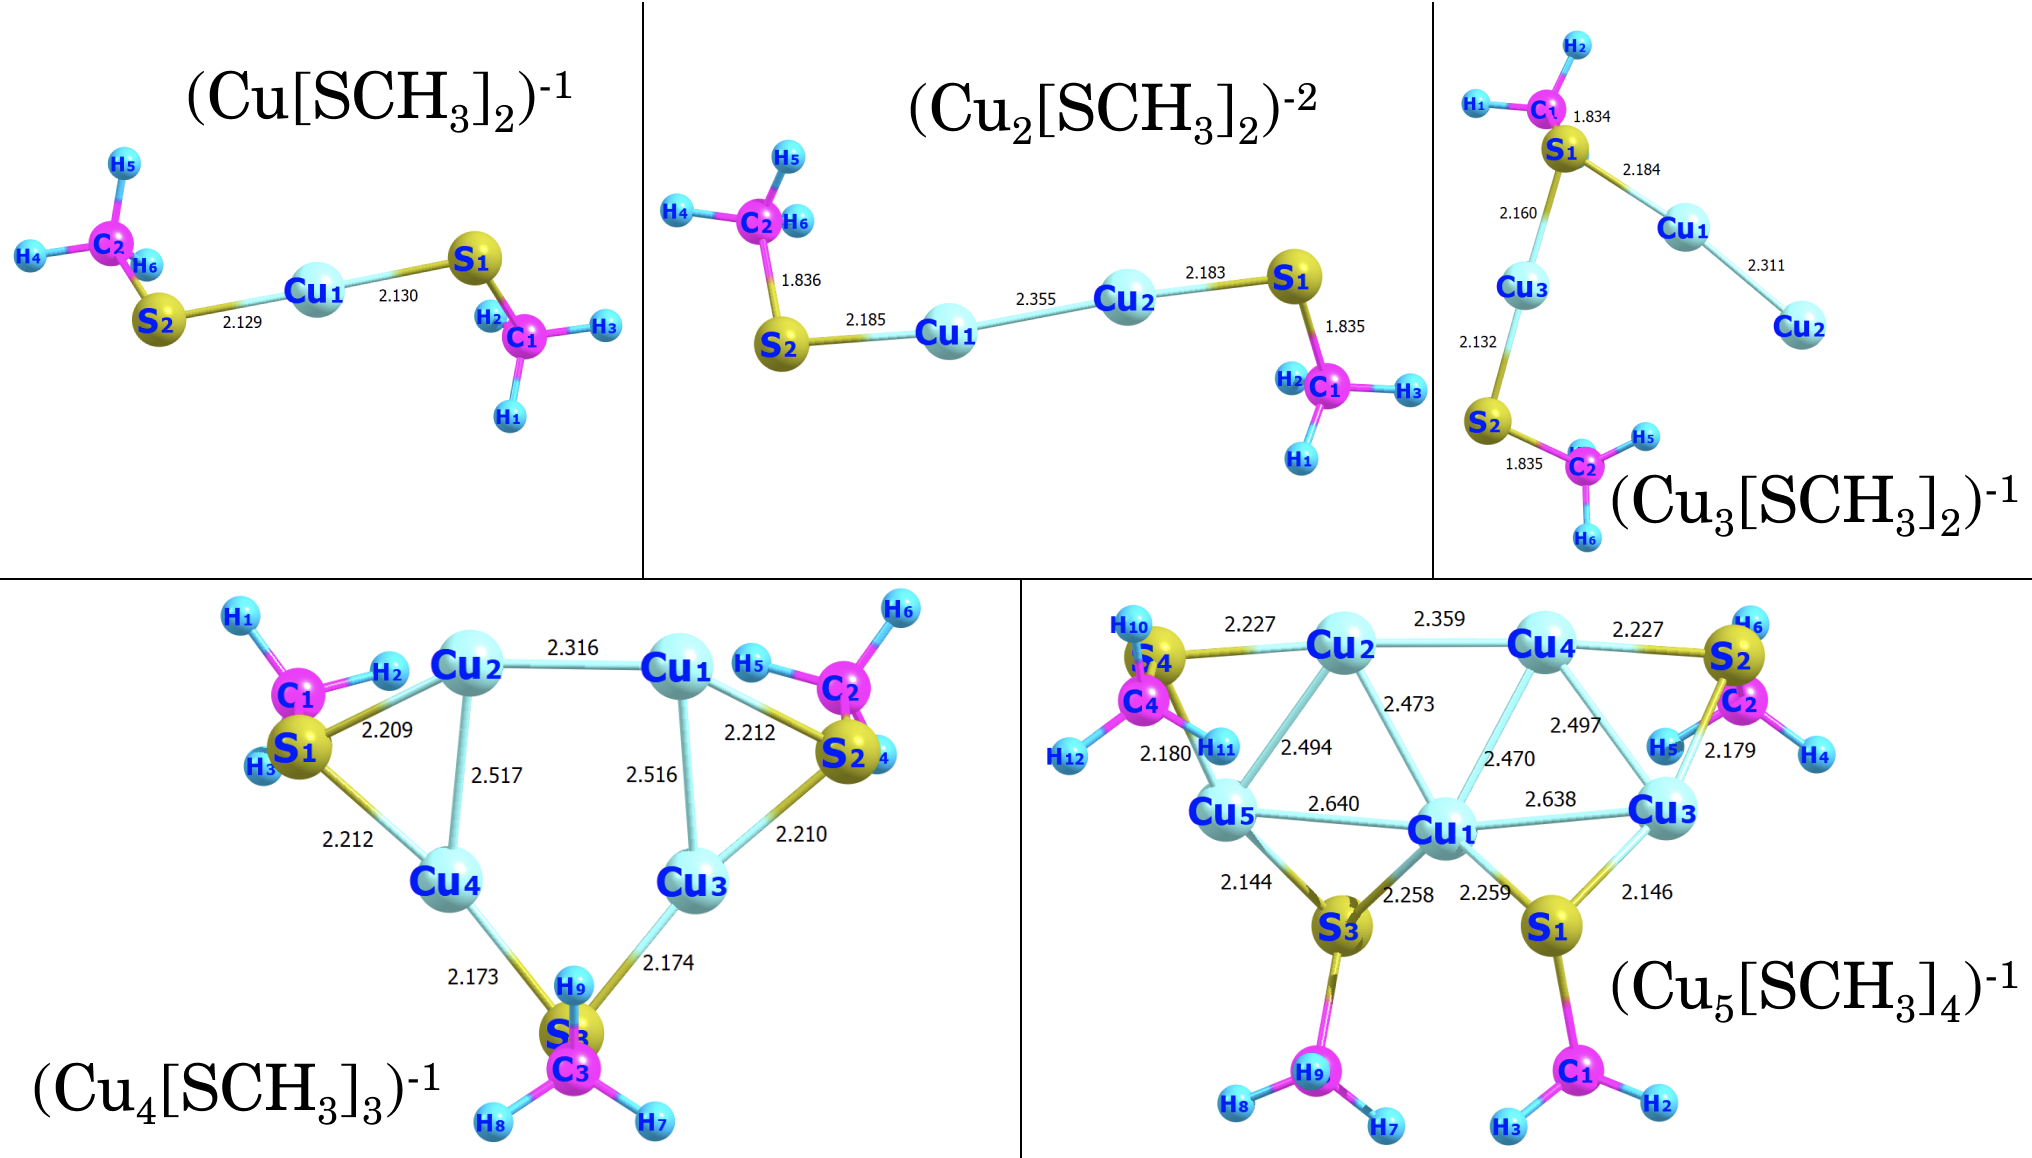
\includegraphics[width=\textwidth, frame]{pictures/opt_SCH3_wat.jpg}
		\caption{Оптимизированные {в воде} геометрии комплексов, стабилизированных метилтиогруппой (метод:\ths MP2\ths def2-TZVP).}
		\label{fig_geoopt_Cys_wat}
	\end{figure}
	
	\begin{figure}[H]
		\centering
		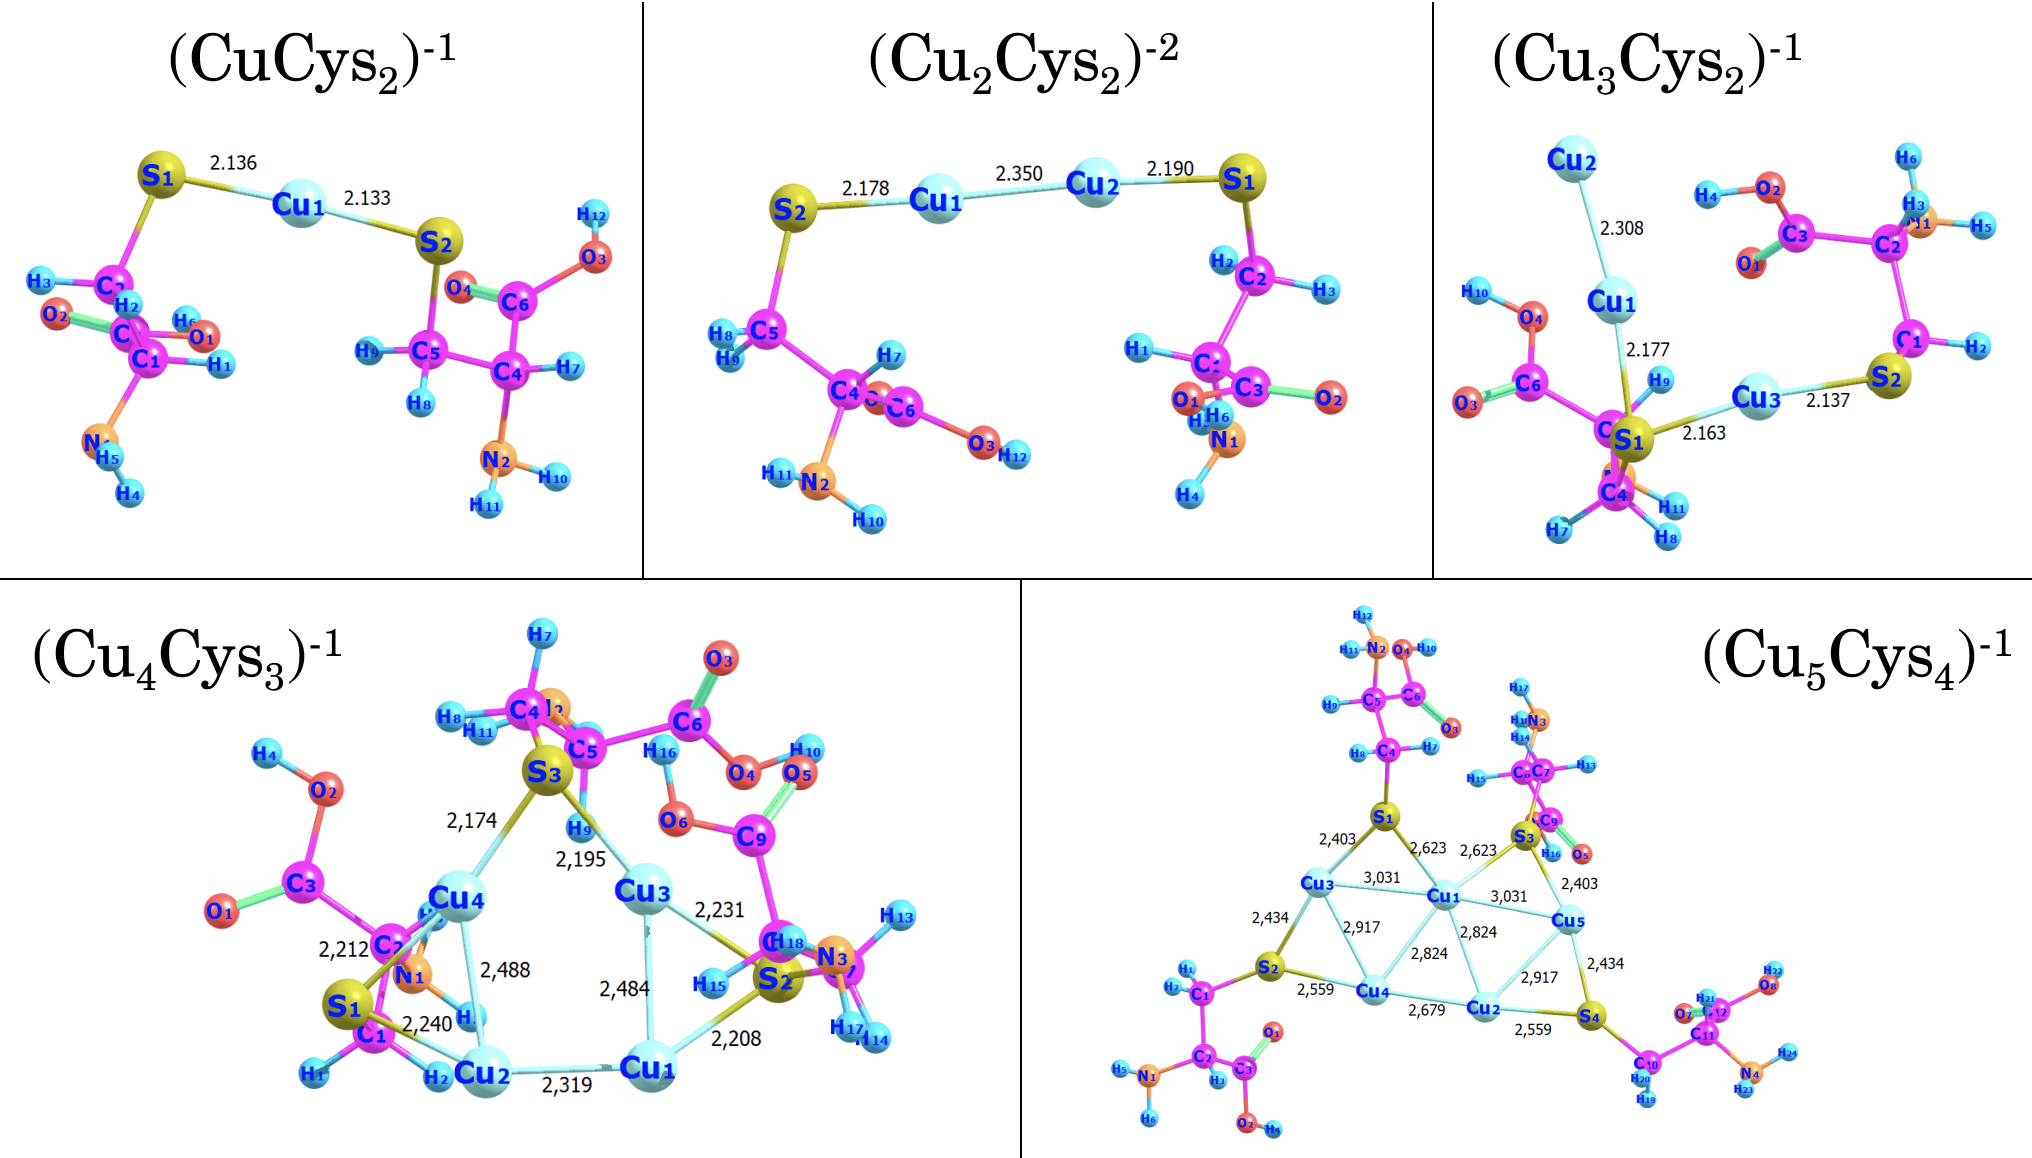
\includegraphics[width=\textwidth, frame]{pictures/opt_Cys_wat.jpg}
		\caption{Оптимизированные {в воде} геометрии комплексов, стабилизированных цистеином (метод:\ths MP2\ths def2-TZVP).}
		\label{fig_geoopt_SCH3_wat}
	\end{figure}
	
	\end{onehalfspace}
\end{document}